% ******************************* PhD Thesis Template **************************
% Please have a look at the README.md file for info on how to use the template

\documentclass[a4paper,12pt,times,numbered,print,index]{Classes/PhDThesisPSnPDF}
\usepackage{CJK}
\usepackage{ctex}
\AtBeginDvi{\pdfmapline{=gbk@UGBK@ <FandolSong}
\pdfmapline{=gbksong@UGBK@ <FandolSong}
\pdfmapline{=gbkkai@UGBK@ <FandolKai}
\pdfmapline{=gbkhei@UGBK@ <FandolHei}
\pdfmapline{=gbkfs@UGBK@ <FandolFang}
\pdfmapline{=gbkli@UGBK@ <STLITI.ttf}
\pdfmapline{=gbkyou@UGBK@ <STHUPO.TTF}
\pdfmapline{=cyberb@Unicode@ <FZSSK.TTF}
\pdfmapline{=unisong@Unicode@ <FZSSK.TTF}
\pdfmapline{=unikai@Unicode@ <FZKTK.TTF}
\pdfmapline{=unihei@Unicode@ <FZHTK.TTF}
\pdfmapline{=unifs@Unicode@ <FZFSK.TTF}
\pdfmapline{=unili@Unicode@ <STLITI.ttf}
\pdfmapline{=uniyou@Unicode@ <STHUPO.TTF}
\pdfmapline{=gbksongsl@UGBK@ <FZSSK.TTF}
\pdfmapline{=gbkkaisl@UGBK@ <FZKTK.TTF}
\pdfmapline{=gbkheisl@UGBK@ <FZHTK.TTF}
\pdfmapline{=gbkfssl@UGBK@ <FZFSK.TTF}
\pdfmapline{=gbklisl@UGBK@ <STLITI.ttf}
\pdfmapline{=gbkyousl@UGBK@ <STHUPO.TTF}
\pdfmapline{=uniheisl@Unicode@ <FZHTK.TTF}
\pdfmapline{=unifssl@Unicode@ <FZFSK.TTF}
\pdfmapline{=unilisl@Unicode@ <STLITI.ttf}
\pdfmapline{=uniyousl@Unicode@ <STHUPO.TTF}}

% ******************************************************************************
% ******************************* Class Options ********************************
% *********************** See README for more details **************************
% ******************************************************************************

% `a4paper'(The University of Cambridge PhD thesis guidelines recommends a page
% size a4 - default option) or `a5paper': A5 Paper size is also allowed as per
% the Cambridge University Engineering Deparment guidelines for PhD thesis
%
% `11pt' or `12pt'(default): Font Size 10pt is NOT recommended by the University
% guidelines
%
% `oneside' or `twoside'(default): Printing double side (twoside) or single
% side.
%
% `print': Use `print' for print version with appropriate margins and page
% layout. Leaving the options field blank will activate Online version.
%
% `index': For index at the end of the thesis
%
% `draftclassic': For draft mode without loading any images (same as draft in book)
%
% `draft': Special draft mode with line numbers, images, and water mark with
% timestamp and custom text. Position of the text can also be modified.
%
% `abstract': To generate only the title page and abstract page with
% dissertation title and name, to submit to the Student Registry
%
% `chapter`: This option enables only the specified chapter and it's references
%  Useful for review and corrections.
%
% ************************* Custom Page Margins ********************************
%
% `custommargin`: Use `custommargin' in options to activate custom page margins,
% which can be defined in the preamble.tex. Custom margin will override
% print/online margin setup.
%
% *********************** Choosing the Fonts in Class Options ******************
%
% `times' : Times font with math support. (The Cambridge University guidelines
% recommend using times)
%
% `fourier': Utopia Font with Fourier Math font (Font has to be installed)
%            It's a free font.
%
% `customfont': Use `customfont' option in the document class and load the
% package in the preamble.tex
%
% default or leave empty: `Latin Modern' font will be loaded.
%
% ********************** Choosing the Bibliography style ***********************
%
% `authoryear': For author-year citation eg., Krishna (2013)
%
% `numbered': (Default Option) For numbered and sorted citation e.g., [1,5,2]
%
% `custombib': Define your own bibliography style in the `preamble.tex' file.
%              `\RequirePackage[square, sort, numbers, authoryear]{natbib}'.
%              This can be also used to load biblatex instead of natbib
%              (See Preamble)
%
% **************************** Choosing the Page Style *************************
%
% `default (leave empty)': For Page Numbers in Header (Left Even, Right Odd) and
% Chapter Name in Header (Right Even) and Section Name (Left Odd). Blank Footer.
%
% `PageStyleI': Chapter Name next & Page Number on Even Side (Left Even).
% Section Name & Page Number in Header on Odd Side (Right Odd). Footer is empty.
%
% `PageStyleII': Chapter Name on Even Side (Left Even) in Header. Section Number
% and Section Name in Header on Odd Side (Right Odd). Page numbering in footer


% ********************************** Preamble **********************************
% Preamble: Contains packages and user-defined commands and settings
% ******************************************************************************
% ****************************** Custom Margin *********************************

% Add `custommargin' in the document class options to use this section
% Set {innerside margin / outerside margin / topmargin / bottom margin}  and
% other page dimensions
\ifsetCustomMargin
  \RequirePackage[left=37mm,right=30mm,top=35mm,bottom=30mm]{geometry}
  \setFancyHdr % To apply fancy header after geometry package is loaded
\fi

% *****************************************************************************
% ******************* Fonts (like different typewriter fonts etc.)*************

% Add `customfont' in the document class option to use this section

\ifsetCustomFont
  % Set your custom font here and use `customfont' in options. Leave empty to
  % load computer modern font (default LaTeX font).
  %\RequirePackage{helvet}

  % For use with XeLaTeX
  %  \setmainfont[
  %    Path              = ./libertine/opentype/,
  %    Extension         = .otf,
  %    UprightFont = LinLibertine_R,
  %    BoldFont = LinLibertine_RZ, % Linux Libertine O Regular Semibold
  %    ItalicFont = LinLibertine_RI,
  %    BoldItalicFont = LinLibertine_RZI, % Linux Libertine O Regular Semibold Italic
  %  ]
  %  {libertine}
  %  % load font from system font
  %  \newfontfamily\libertinesystemfont{Linux Libertine O}
\fi

% *****************************************************************************
% **************************** Custom Packages ********************************

% ************************* Algorithms and Pseudocode **************************

%\usepackage{algpseudocode}
\usepackage{algorithm}
\usepackage{algorithmic}

% ********************Captions and Hyperreferencing / URL **********************

% Captions: This makes captions of figures use a boldfaced small font.
%\RequirePackage[small,bf]{caption}

\RequirePackage[labelsep=space,tableposition=top]{caption}
\renewcommand{\figurename}{Fig.} %to support older versions of captions.sty
\newcommand{\eqname}[1]{Eq. {#1}}
\newcommand{\algoname}[1]{Algo.{#1}}
\newcommand{\tblname}[1]{Table {#1}}
% *************************** Graphics and figures *****************************

%\usepackage{rotating}
%\usepackage{wrapfig}

% Uncomment the following two lines to force Latex to place the figure.
% Use [H] when including graphics. Note 'H' instead of 'h'
%\usepackage{float}
%\restylefloat{figure}

% Subcaption package is also available in the sty folder you can use that by
% uncommenting the following line
% This is for people stuck with older versions of texlive
%\usepackage{sty/caption/subcaption}
\usepackage{subcaption}

% ********************************** Tables ************************************
\usepackage{booktabs} % For professional looking tables
\usepackage{multirow}

\usepackage{multicol}
\usepackage{longtable}
\usepackage{tabularx}


% *********************************** SI Units *********************************
\usepackage{siunitx} % use this package module for SI units


% ******************************* Line Spacing *********************************

% Choose linespacing as appropriate. Default is one-half line spacing as per the
% University guidelines

% \doublespacing
% \onehalfspacing
% \singlespacing


% ************************ Formatting / Footnote *******************************

% Don't break enumeration (etc.) across pages in an ugly manner (default 10000)
%\clubpenalty=500
%\widowpenalty=500

%\usepackage[perpage]{footmisc} %Range of footnote options


% *****************************************************************************
% *************************** Bibliography  and References ********************

%\usepackage{cleveref} %Referencing without need to explicitly state fig /table

% Add `custombib' in the document class option to use this section
\ifuseCustomBib
  \RequirePackage[square, sort, numbers, authoryear]{natbib} % CustomBib

  % If you would like to use biblatex for your reference management, as opposed to the default `natbibpackage` pass the option `custombib` in the document class. Comment out the previous line to make sure you don't load the natbib package. Uncomment the following lines and specify the location of references.bib file

  %\RequirePackage[backend=biber, style=numeric-comp, citestyle=numeric, sorting=nty, natbib=true]{biblatex}
  %\bibliography{References/references} %Location of references.bib only for biblatex

\fi

% changes the default name `Bibliography` -> `References'
\renewcommand{\bibname}{References}


% ******************************** Roman Pages *********************************
% The romanpages environment set the page numbering to lowercase roman one
% for the contents and figures lists. It also resets
% page-numbering for the remainder of the dissertation (arabic, starting at 1).

\newenvironment{romanpages}{
  \setcounter{page}{1}
  \renewcommand{\thepage}{\roman{page}}}
{\newpage\renewcommand{\thepage}{\arabic{page}}}


% ******************************************************************************
% ************************* User Defined Commands ******************************
% ******************************************************************************

% *********** To change the name of Table of Contents / LOF and LOT ************

%\renewcommand{\contentsname}{My Table of Contents}
%\renewcommand{\listfigurename}{My List of Figures}
%\renewcommand{\listtablename}{My List of Tables}


% ********************** TOC depth and numbering depth *************************

\setcounter{secnumdepth}{2}
\setcounter{tocdepth}{2}


% ******************************* Nomenclature *********************************

% To change the name of the Nomenclature section, uncomment the following line

%\renewcommand{\nomname}{Symbols}


% ********************************* Appendix ***********************************

% The default value of both \appendixtocname and \appendixpagename is `Appendices'. These names can all be changed via:

%\renewcommand{\appendixtocname}{List of appendices}
%\renewcommand{\appendixname}{Appndx}

% *********************** Configure Draft Mode **********************************

% Uncomment to disable figures in `draftmode'
%\setkeys{Gin}{draft=true}  % set draft to false to enable figures in `draft'

% These options are active only during the draft mode
% Default text is "Draft"
%\SetDraftText{DRAFT}

% Default Watermark location is top. Location (top/bottom)
%\SetDraftWMPosition{bottom}

% Draft Version - default is v1.0
%\SetDraftVersion{v1.1}

% Draft Text grayscale value (should be between 0-black and 1-white)
% Default value is 0.75
%\SetDraftGrayScale{0.8}


% ******************************** Todo Notes **********************************
%% Uncomment the following lines to have todonotes.

%\ifsetDraft
%	\usepackage[colorinlistoftodos]{todonotes}
%	\newcommand{\mynote}[1]{\todo[author=kks32,size=\small,inline,color=green!40]{#1}}
%\else
%	\newcommand{\mynote}[1]{}
%	\newcommand{\listoftodos}{}
%\fi

% Example todo: \mynote{Hey! I have a note}


% ************************ Thesis Information & Meta-data **********************
% Thesis title and author information, refernce file for biblatex
% ************************ Thesis Information & Meta-data **********************
%% The title of the thesis
\title{Writing your thesis in \texorpdfstring{\\ \LaTeX2e}{LaTeX2e}}
%\texorpdfstring is used for PDF metadata. Usage:
%\texorpdfstring{LaTeX_Version}{PDF Version (non-latex)} eg.,
%\texorpdfstring{$sigma$}{sigma}

%% Subtitle (Optional)
%\subtitle{Using the template}

%% The full name of the author
\author{Author's name}
%\vspace{2cm}
\supervisor{Supervisor's name}
%% Department (eg. Department of Engineering, Maths, Physics)
%%\dept{CCNU Wollongong Joint Institute}

%% University and Crest
%%\university{Central China Normal University}
% Crest minimum should be 30mm.
\crest{
\includegraphics[width=0.4\textwidth]{1}}
%% Use this crest, if you are using the college crest
%% Crest long miminum should be 65mm
%\crest{
\includegraphics[width=0.45\textwidth]{University_Crest_Long}}

%% College shield [optional]
% Crest minimum should be 30mm.
%\collegeshield{
\includegraphics[width=0.2\textwidth]{CollegeShields/Kings}}

%% You can redefine the submission text:
% Default as per the University guidelines:
% ``This dissertation is submitted for the degree of''
%\renewcommand{\submissiontext}{change the default text here if needed}

%% Full title of the Degree
\degreetitle{Master of Engineering}

%% College affiliation (optional)
\college{Central China Normal University Wollongong Joint Institute}
\university{Central China Normal University}

%% Submission date
% Default is set as {\monthname[\the\month]\space\the\year}
%\degreedate{September 2014}

%% Meta information
\subject{LaTeX} \keywords{{LaTeX} {Thesis} {Engineering} {Central China Normal University}}


% ***************************** Abstract Separate ******************************
% To printout only the titlepage and the abstract with the PhD title and the
% author name for submission to the Student Registry, use the `abstract' option in
% the document class.

\ifdefineAbstract
 \pagestyle{empty}
 \includeonly{Declaration/declaration, Abstract/abstract}
\fi

% ***************************** Chapter Mode ***********************************
% The chapter mode allows user to only print particular chapters with references
% Title, Contents, Frontmatter are disabled by default
% Useful option to review a particular chapter or to send it to supervisior.
% To use choose `chapter' option in the document class

\ifdefineChapter
 \includeonly{Chapter3/chapter3}
\fi

% ******************************** Front Matter ********************************
\begin{document}
\begin{CJK*}{UTF8}{song}
\frontmatter

\begin{titlepage}
  \maketitle
\end{titlepage}



% ******************************* Thesis Declaration ***************************
% Do not change the following content
\begin{declaration}
I hereby declare that except where specific reference is made to the work of
others, the contents of this thesis are original and have not been
submitted in whole or in part for consideration for any other degree or
qualification in this, or any other university. This thesis is my own
work and contains nothing which is the outcome of work done in collaboration
with others, except as specified in the text and Acknowledgments.

\end{declaration}



% Author and date will be inserted automatically from thesis.tex \author \degreedate



% ************************** Thesis Abstract *****************************
% Use `abstract' as an option in the document class to print only the titlepage and the abstract.

%Please list 3-5 keywords, and replace them with "keyword1", "keyword2", "keyword3",...
\begin{abstract}{Graph Neural Network}{Knowledge Point Labeling}{Knowledge Tracking}{Recommended Exercises}{}
    After 2010, artificial intelligence technology has become a research hotspot in computer technology, causing explosive development in related industries. Various algorithm innovations, theoretical breakthroughs and model applications have emerged one after another and have also caused intelligent innovations in various industries. Among them, the application of artificial intelligence technology in the field of education has led to the emergence of the concept of intelligent education. Among them, adaptive learning is one of the more popular application fields in intelligent education\cite{ma2017adalearn}. Adaptive learning tracks students' learning status by combining big data analysis based on massive student group learning data and learning data based on individual target students. It develops a personalized learning plan based on students' characteristics and learning goals\cite{soltani2019adaptive}. This technology can systematically alleviate the current contradiction between the scarcity and uneven distribution of domestic educational resources. It can also reduce the burden on education practitioners and students and has good development prospects and commercial value. More and more artificial intelligence research teams and intelligent education technology companies in the market start to focus on developing and applying adaptive learning tools. Simultaneously, many education companies have begun to use adaptive learning as the main core function or main selling point of their products. Adaptive educational technology can combine and analyze students' knowledge mastery, gaps and individual learning abilities so as to have the most suitable learning path and learning resources such as exercises, materials, and knowledge points to students. The system will automatically adjust the difficulty of pushing learning resources according to the students' knowledge status to prevent the diminished interest in learning caused by over-distress or over-easiness. Combined with manual tutoring, teachers can also analyze each student's knowledge gap according to the learning status evaluation report tracked and calculated by the system and adjust the education and learning plan adaptively to realize the personalized teaching provision program assisted by the system. Therefore, adaptive learning is one of the potential practical solutions to "teaching students based on their mastery and individual characteristics" in online education. This article aims to design an exercise recommendation system that combines knowledge point labelling, knowledge tracking, and resource recommendation technology to propose an adaptive learning program in exercise recommendation.

    This article takes high school mathematics as the primary research object. In high school mathematics, exercises are the primary means to improve learning ability. However, current high school mathematics has problems such as too large exercise database, high repetition and disordered organization, among which there are quite a lot of similar or repeated exercises. In traditional high school mathematics education, some students learn through problem tactics. However, they tend to concentrate on the more proficient knowledge points for much practice, resulting in a little effect. Therefore, experienced teaching staff are required to recommend exercises. This method is often done through manual recommendation, and the teacher pushes them to the students in a class through exercises classification and exercises summary. This method requires much manual work, relies on experts' prior knowledge, and does not make recommendations for students' individualized knowledge mastery. The recommendation effect is plough to improve this kind of situation. The application of knowledge tracking technology can recommend exercises based on the students' knowledge mastery. This article aims to design an exercise recommendation system that combines knowledge point labelling, knowledge tracking, and resource recommendation technology to form an intelligent adaptive learning solution in exercise recommendation.

    The high school math learning question recommendation system proposed in this paper includes three modules: the exercise knowledge point labelling module, the knowledge tracking module, and the recommendation module. The exercise knowledge point mining module's function is to label the knowledge points for the exercises that have not been marked so as to replace the traditional manual labelling with machine automation. Knowledge point labelling is the pre-work of exercise recommendation, and the exercises that have been labelled with knowledge can be used as the exercises of the knowledge tracking system to be embedded in the learning data source. The knowledge tracking module obtains and calculates the student's knowledge state's representation by tracking the student's question record. The knowledge state vector represents the student's knowledge and skill mastery and is the core part of the entire system. In the final exercise recommendation module, input the knowledge vector and exercise embedding representation obtained in the previous period, and combine collaborative filtering and related recommendation models to perform preliminary filtering and fine recommendation of exercises, thereby realizing exercise recommendation based on knowledge status.
    \begin{itemize}
        \item In the knowledge point annotation module, a graph convolutional neural network is used to train the label annotation classifier. Use Bi-LSTM to mine the exercise text information, embed the exercise text as the input of the label classifier group, and output a set of label classification results.
        \item In the knowledge tracking module, a graph attention network is used to learn the knowledge relationship of exercises. The embedding vector is output through the Transformer-based Encoder model to output a knowledge state vector, and then the exercise embedding vector and the knowledge state vector are used as the Transformer-based Decoder The input and output of the model predict the answer to the next exercise.
        \item In the exercise recommendation module, a recall model based on collaborative filtering and a ranking model based on MLP are used. In the recall phase, collaborative filtering is used to find the problem sets of other students with similar knowledge status. In the sorting phase, the knowledge status vector obtained from the knowledge tracking module and the label vector of the exercises are input into the final ranking model, and a priority sequence of exercise recommendation is input.
    \end{itemize}

    This paper implements the above three modules by designing different neural network models and algorithms. It is innovative in algorithm design and experimental verification methods. After experimental verification, it has better performance than similar models.
\end{abstract}

% ************************** Thesis Abstract *****************************
% Use `abstract' as an option in the document class to print only the titlepage and the abstract.

%Please list 3-5 keywords, and replace them with "keyword1", "keyword2", "keyword3",...
\begin{abstractC}{图神经网络}{知识点标注}{知识追踪}{习题推荐}{}
    2010年后,人工智能技术逐渐成为计算机技术领域的研究热点。尤其是机器围棋手AlphaGo的问世,引发了业界对于人工智能前景的极大关注。这带来行业的爆发式发展,也提出了大量的研究课题。在人工智能相关研究中,各种算法创新、理论突破和模型应用层出不穷,为各个行业的智能化奠定了基础。人工智能技术在教育领域的应用也催生了智能教育概念的出现。其中,自适应学习是智能教育中的热门的应用领域之一\cite{ma2017adalearn}。自适应学习模型一般是通过结合对海量学生群体学习数据的大数据分析和对目标学生个体数据的精准化数据分析来追踪学生的学习状态,从而针对学生的个体特征和知识掌握熟练度来生成个性化学习路径\cite{soltani2019adaptive}。自适应学习技术可以将以往需要大量人工劳动的学生评估和教学计划等工作,通过自动化机器学习算法来完成,这可以系统性缓解目前国内教育资源稀缺和分配不均的问题也可以减轻教育从业者和学生的负担。它也具有极大的的发展前景和商业价值,市面上也有越来越多的人工智能研究团队和智能化教育技术公司专注于自适应学习工具的研发和应用,部分智能教育科技公司已开始将自适应学习用作其产品要核心功能或主要卖点。自适应教育技术可以综合分析学生个体层面的学习能力、知识熟练度和群体层面的热门学习资源、易错题等,从而可以将最适合的学习路径和学习资源例如习题、资料、知识点推送给学生。系统会根据学生的知识状态自动调整推送学习资源的知识侧重点,防止重复练习已经掌握的知识点或者缺乏练习未掌握的知识点。一方面,教师可以根据系统输出的数据或可视化图表来制作每个学生的学习状态评估报告分析整个班级的知识掌握熟练度,适应性地调整总体教学计划。另一方面,学生可以通过系统来分析自己的知识薄弱项,从而针对性的进行习题训练。因此,适应性学习是在线教育中``学生知识掌握状态自动评估和教学方案生成''问题潜在可行解决方案之一。

    本文以高中数学学科为主要研究背景,目的是提出一种基于知识追踪的高中数学习题推荐模型。在高中数学学科中,练习习题为学生主要的学习能力提高手段。但是目前高中数学教学中,教师或学生需要从庞大的习题库中去寻找合适的习题进行练习,它们往往存在过于庞大、重复度高和组织混乱等问题。在习题库中存在相当多低质量的未标注知识点的习题,需要人工进行知识点标注。有部分学生通过题海战术来进行学习,但这样效率较低,且往往出现熟悉知识点的重复练习和不熟悉知识点的缺乏练习等情况。为了提高学生进行习题练习的效果,从而提升知识掌握的熟练度和全面性,需要经验丰富的教学人员进行学生知识状态分析,从习题库中筛选出合适的习题进行推荐。该方法人工工作量大,依赖专家先验知识,且包含大量的重复性工作,因此存在不经济且低效的问题。此外,传统习题推荐以学生群体为单位,没有针对特定学生的知识掌握情况进行推荐,也没有考虑不同学生的学习能力不同的问题,因此导致推荐的效果精细度较差。为了改善传统习题推荐方法存在的问题,可以通过应用知识追踪技术来追踪学生的学习情况,从而针对性地进行自动化习题推荐。本文的目标在于设计一个基于知识点标注、知识追踪和资源推荐技术的习题推荐系统,从而推出一个在习题推荐方面的智能自适应学习的解决方案。

    本文提出的高中数学习题推荐系统包括三个模块,分别为习题知识点标注模块、知识追踪模块和推荐模块。习题知识点标签模块的作用是为未标注知识点的习题进行知识点标注,从而将传统的人工知识点标注以自动化的形式代替。知识点标注是习题推荐的前置工作,经过知识标注的习题可以作为习题推荐系统的数据源。知识追踪模块通过追踪学生的习题练习记录,计算学生的知识熟练度状态向量,它是学生对于学科知识点、概念和技能的掌握度的表征。知识追踪是整个系统的核心部分。在最后的习题推荐模块,具有召回和排序两个阶段,前者应用于习题库上应用多种召回策略对习题进行快速筛选,生成推荐候选习题集合,后者输入该集合在排序阶段输入知识追踪系统中进行精细化推荐排序,生成最终的推荐结果。
    \begin{itemize}
        \item 第二章提出了一种基于双向LSTM与图神经网络的高中数学习题多知识点标注方法,习题知识点标注模块包含习题文本挖掘和多知识点标签分类两个子模块。由于习题库的大多数习题只包含文本信息等非结构化数据,因此本文主要通过习题文本挖掘的方式来进行知识点提取。它应用了加入注意力机制的双向LSTM网络来进行习题文本挖掘,习题首先经过分词、清洗、正则化等预处理步骤,得到词序列的同时过滤掉大量的无关信息的干扰。接下来,通过word2vec的方式而非简单的one-hot编码方式来作为学习词嵌入向量,这样做可以防止输入词向量矩阵稀疏带来的维数灾难等问题。而且,通过嵌入学习的方式,也可以表征词向量间的隐藏依赖关系,有利于构建知识点间依赖关系。之后,通过双向LSTM模型进行文本信息抽取,能够更好地解决文本中上下文元素长程依赖的问题。另外,为了在分类模型上捕捉知识点间依赖关系,本文提出了一个基于图卷积网络(GCN)的多标签知识点标注模型,每个标签由知识点的图嵌入表示,经过多轮迭代学习,将标签图映射为一组内在依赖的知识点分类器。随后,将前一个子网络提取的习题文本词向量输入知识点分类器组,得出多知识点预测概率向量,从而实现多知识点标签标注任务。实验阶段,通过在自制的高中数学习题数据集上进行实验,将本论文提出的方法与一系列基准模型进行对比,并采用一系列多标签分类指标来进行模型性能比较和评估。实验结果显示该方法在知识点关系较为复杂的习题集上取得了更加优越的性能。
        \item 第三章提出了基于图注意力网络(GAT)和Transformer架构的知识追踪模型。该模型通过图注意力网络来学习习题间在知识点层面上的复杂关联关系,针对传统的知识追踪模型对于习题间知识点复杂关联关系表征不足的缺陷进行了优化。它解决了如下问题,(1)传统模型将知识点建模为相互独立的关系或者简化的的概率依赖关系,而忽略了知识点间复杂的图状关系,从而对于知识点依赖关系复杂的数据表现不佳。(2)传统模型无法输出学生的知识状态,而只能输出对于下一道习题的回答正确概率,从而难以结合推荐模型进行习题推荐。本文提出的模型结合图注意力网络对于非欧式空间的数据和图的强大表征学习能离和Transformer模型对于序列化习题练习数据的远程依赖的注意力机制建模能力,在处理较长的习题练习记录和知识关系复杂的习题数据集上具有更佳的性能。实验阶段,通过在若干个知识追踪领域公开数据集上进行实验,将本论文提出的模型与基准模型进行性能对比。实验结果显示,在公开数据集上,本模型相对于大多数模型在评估参数上都取得了较优或者相当的结果。
        \item 第四章提出了基于召回-排序两阶段的数学习题推荐模型。第一阶段为召回模型,它是一个基于多召回策略的混合模型,它具有多路召回和融合两个过程。在多路召回过程,采用了基于协同过滤、热门度、用户偏好等多个召回策略用于分别生成习题推荐候选集合。然后在融合过程,将这些候选集合进行加权排序合并,形成一个最终的习题推荐候选集合。第二个阶段为基于知识追踪的推荐项排序模型,将前一阶段获取的习题候选集合中的每个习题输入到前一章提出的知识追踪模型,进行正确率预测,将最容易出错的习题的作为优先级最高的推荐项。该模型主要解决的是传统模型往往需要用户主动评分来进行推荐模型构建,而无法基于用户的知识掌握熟练度状态进行高效推荐的问题。经过在公开数据集上的性能测试和与baseline模型的对照实验,提出的模型在对于学生的掌握薄弱知识的追踪性能较为优越,并能依据追踪得到的的知识掌握熟练度状态推荐合适的习题。
    \end{itemize}

    本文通过分析系统的需求,将整个推荐系统合理化分为多个模块,并针对各个模块设计了不同的神经网络模型和算法来实现和优化上述三个模块,在算法设计和实验验证方法方面都具有一定的创新性。经过实验验证,具备相对于同类模型更好的性能。
\end{abstractC}

% ************************** Thesis Acknowledgements **************************

\begin{acknowledgments}

%%Write the acknowledgments here ...


\end{acknowledgments}

% ************************** Thesis Abstract *****************************
% Use `abstract' as an option in the document class to print only the titlepage and the abstract.
\begin{publication}
List your publications here...

Please remove this page if you do not have any...


\end{publication}



% *********************** Adding TOC and List of Figures ***********************

\tableofcontents

\listoffigures

\listoftables

% \printnomenclature[space] space can be set as 2em between symbol and description
%\printnomenclature[3em]

\printnomenclature

% ******************************** Main Matter *********************************
\mainmatter

%*******************************************************************************
%*********************************** First Chapter *****************************
%*******************************************************************************

\chapter{Introduction}  %Title of the First Chapter

\ifpdf
    \graphicspath{{Chapter1/Figs/Raster/}{Chapter1/Figs/PDF/}{Chapter1/Figs/}}
\else
    \graphicspath{{Chapter1/Figs/Vector/}{Chapter1/Figs/}{Chapter1/Figs/PDF/}}
\fi


%********************************** %First Section  **************************************
\section{Research Background and Significance} %Section - 1.1
%人工智能的技术研究和商业化应用部署在近年来的发展显示了一种加速的趋势。各种基于人工智能和大数据分析相关算法的部署上线在加速企业、组织数字化,改善产业链结构和提高信息利用效率方面发挥了积极作用。教育行业作为传统的服务行业,也存在相当大的智能化革命的空间。在传统教育模式中,学生群体往往被分为班级这种基础教育单元。因而在一个班级中,所有的教学活动的粒度与班级的大小相当,这导致学生所学习的内容与其需求不完全匹配。也即,学生已经掌握的知识点过度练习或者未掌握的知识点缺乏练习。这造成了学生出现厌学、焦虑等状况,对其学习效率和学习效果造成了较大影响。另一方面,对于教师而言,普遍性的个体知识状态精细监测和评估需要巨大的工作量,因此教师往往只关注一部分学生,导致多数学生的学习情况被忽略。这对于学生的学习积极性和学习状况具有较大的影响。

The development of technological research and commercial application deployment of artificial intelligence has shown an accelerating trend in recent years. The deployment of various algorithms related to AI and big data analytics based on artificial intelligence plays a positive role in accelerating enterprises and organizations' digitization, improving industry chains' structure, and increasing information utilization efficiency. As a traditional service industry, the education industry also has considerable prospects for an intelligent revolution. In traditional education models, student groups are often divided into basic education units like classes. Therefore, in a class, the granularity of all teaching activities is equivalent to the class size, which leads to the fact that the content of students' learning does not entirely match their needs. The knowledge points that the students have mastered are over-practice, or the knowledge points that the students have not mastered lack practice. This has caused students to be tired of learning, anxiety, and other conditions, significantly impacting their learning efficiency and learning effect. On the other hand, for teachers, generalized detailed monitoring and evaluation of individual knowledge status require a considerable workload, so teachers often only pay attention to a part of the students, leading to the neglect of most students' learning situation, which has a more significant impact on students' learning enthusiasm and learning conditions.

%近年来,中国发布了一系列促进人工智能在教育领域的应用的政策。通过人工智能技术来进行学生的学习情况监测和追踪,可以解放教师的劳动力,还可以解决传统人工教育中难以解决的问题,从而大大改善教育质量和效率,实现智慧教育。在智慧教育中,自适应学习是一个已经实践验证过的模型,它已经拥有了许多商业化部署的成功案例。相当多的在线教育平台已经部署了不同领域的自适应学习教育系统服务。它运用数据分析、机器学习和自动化等技术,通过分析学生的学习行为数据,自动地对学生进行知识状态的评估和追踪。此外,该系统结合学生的潜能、擅长领域等等个性化信息,向学生提供学习路径规划和学习资源推荐服务。它在降低教师工作压力的同时,能够提升教师的教学质量,也能够有效地帮助学生提升学习的效率。习题推荐系统是一个自适应学习的实现,它包括学习者知识掌握熟练度建模和习题推荐两个部分。知识掌握熟练度建模的一般模式为,输入学习者的学习交互记录例如做题记录、测验记录等语义记录,捕获学习者的学习特征,实现对于其知识掌握熟练度的动态追踪。习题推荐部分则通过分析学习者的知识掌握熟练度模型,推荐与学习者的知识掌握相对薄弱的部分最相关的习题。

In recent years, China has released a series of policies to promote artificial intelligence in education. AI technology for student learning monitoring and tracking can free up teachers' labor and solve problems that are difficult to solve in traditional manual education, thus significantly improving the quality and efficiency of education and realizing smart education. In smart education, adaptive learning is a model that has been proven in practice, and it already has many successful cases of commercial deployment~\cite{chen2018recommendation}. A considerable number of online education platforms have deployed adaptive learning education system services in different domains. It uses data analytics, machine learning, and automation to automatically assess and track students' knowledge status by analyzing their learning behavior data. Besides, the system provides students with learning path planning and learning resource recommendation services by combining personalized information such as students' potential and areas of expertise~\cite{soltani2019adaptive}. It can improve teachers' teaching quality while reducing teachers' work pressure and effectively improve their learning efficiency. The exercise recommendation system implements an adaptive learning model, including learner knowledge mastery proficiency modeling and exercise recommendation. The general model of knowledge mastery modeling is to input the semantic records of learners' learning interactions such as question records, quiz records to capture learners' learning characteristics and achieve the dynamic tracking of their knowledge mastery proficiency. The exercise recommendation part analyzes the learners' knowledge mastery proficiency model and recommends exercises relevant to the learners' relatively weak knowledge mastery.

%高中数学学科是高中阶段相对较难的一门科目。目前,在高中数学学科中,知识点繁杂而且具有紧密的内在联系,对应的习题库也庞大而混乱。导致许多学生不知道如何去合理评估自己的知识掌握度从而有针对性地练习,导致``题海战术''的出现。这对于学生的学习兴趣和自信心有负面的影响。本文把高中数学学科作为研究背景,目的是提出一种实时追踪学生数学知识掌握情况,并依照学生的知识状态进行习题推荐的系统。该系统分为三个部分,第一个部分对习题进行知识点标注,作为习题推荐系统的数据准备部分,第二部分是核心的知识追踪模型,它通过输入学生的做习题记录来追踪知识熟练度状态,第三部分是系统的功能部分,它通过知识追踪模型输出的学生知识熟练度针对性地推荐习题。该系统可以有效地实现自适应学习的目标。

High school mathematics is a relatively tricky subject at the high school level. In high school mathematics, the knowledge points are complicated and closely interconnected, and the corresponding library of exercises is extensive and confusing. As a result, many students do not know how to reasonably assess their knowledge and practice in a targeted manner, leading to the emergence of ``excessive practicing tactics'', which hurts students' interest in learning and self-confidence. The purpose of this thesis is to propose a system for tracking students' knowledge of mathematics in real-time and recommending exercises according to their knowledge status. The system is divided into three parts, the first part is the knowledge labeling of the exercises as the data preparation part of the exercise recommendation system, the second part is the core knowledge tracing model, which tracks the knowledge proficiency status by inputting students' records of doing exercises, and the third part is the functional part of the system, which recommends exercises targeted by students' knowledge proficiency output from the knowledge tracing model. The system can effectively achieve the goal of adaptive learning.

%********************************** %Second Section  *************************************
\section{Related Works}



%本文的研究课题为高中数学习题推荐系统,

%如wang等人提出结合神经网络的认知诊断模型NeuralCD,在预测精度和可解释性上均有所提升。一种流行的方法是是通过认知诊断的方式来对学生的知识掌握状态进行评估,然后基于学生的知识状态来进行对应的习题推荐。

%第一个部分为基于图神经网络和自然语言处理的习题知识点标注,第二个部分为基于图注意力网络与Transformer的知识追踪模型,第三个部分为基于协同过滤和神经网络的习题推荐模块, 的知识跟踪与推荐系统等。因而本文涉及的技术包括高中数学图神经网络,自然语言处理,多标签分类,推荐系统等研究课题, 接下来,本节将回顾这些技术的研究现状。
This thesis's research topic is a recommendation system for high school mathematics exercises, for which there have been several studies and applications. A popular approach is to evaluate and track students' knowledge mastery status using cognitive diagnosis and then recommend corresponding exercises based on students' knowledge status. For example, wang et al.\ proposed NeuralCD~\cite{wang2020neural}, a cognitive diagnostic model combined with neural networks, which has improved in both prediction accuracy and interpretability. There are also some improvements to the model, such as Huang et al.~\cite{huang2017hcdm} applying multilevel structure into higher-order latent features to extend the original model into a multilevel higher-order cognitive diagnostic model.


The first part of this thesis is a graph neural network and Attentional Bi-LSTM based knowledge point labeling for high school math exercises, the second part is a graph attention network and Transformer based knowledge tracing model, and the third part is a matching and ranking based exercise recommendation module. Thus, the techniques covered in this thesis include high school mathematics subjects, graph neural networks, natural language processing, multi-label classification, recommendation systems, and other research topics. Next, this section reviews the current state of research on these techniques.

\subsection{High School Mathematics}
%无论在基础教育还是科学研究中,数学都是一门必要的的学科。数学是一门专门研究数量与空间形式之间关系的科学,其符号系统更加完整,公式结构清晰独特,文字和图像等语言表达方式也更加生动直观。在数学学科中,知识结构和认知结构的建立对于该学科的学习起着相当重要的作用。``认知结构''表示在人大脑当中陈述性知识的组织形式,而经过学习内化后的认知结构通过网络结构或图形展示出来的就是知识结构~\cite{tanujaya2017relationship}。学习者所需要学习的知识内容大多来源于前人在实践活动中的经验总结,其学习的过程就是对这些归纳好的知识进行认知学习,并不断对知识的结构进行消化、调整、重组,从而构建更为完善和适合自己的知识结构的过程,也是一个与创新思维结合的过程。在数学学科中,知识的掌握往往来自于实践,例如习题练习、证明推导等等。数学学科作为中学阶段的主要科目,具有高度抽象性、严密逻辑性与广泛应用性等特点。该学科知识体系是利用众多的抽象性知识概念建立起来的,并借助对这些概念知识进行学习与思维拓展,形成新的抽象性概念知识。此外,数学逻辑性十分严密,因为数学学科当中得出的任何结论,都需要经过严密的逻辑推理与严格的证明才能被认为是合理的。它是我们参与社会实践活动或科学研究的重要手段和工具,在各行各业以及社会的各个领域当中都离不开对数学的学习。数学知识点之间也具有内在关联性,因而它们可以在具体学习过程中根据特定的逻辑顺序进行安排和学习。这些内在关联关系可以分为同义关系、前驱关系、后继关系、包含关系、兄弟关系、对立关系等几种。通过对知识点进行分析,可以建立知识点关联网络,便于进行后续的知识状态追踪。


Mathematics is an essential subject in both primary education and scientific research. Mathematics is a science devoted to studying relationships between quantities and spatial forms, with a complete system of symbols, a clear and unique structure of formulas, and more vivid and intuitive verbal expressions such as words and images. In mathematics, the establishment of knowledge structure and cognitive structure plays a considerable role in learning the subject. The ``cognitive structure'' denotes the organization of declarative knowledge among the human brain, while the cognitive structure internalized through learning and displayed through network structures or graphics is the knowledge structure~\cite{tanujaya2017relationship}. Most of the knowledge contents that learners need to learn come from the experience summaries of previous people in practical activities, and the process of their learning is the cognitive learning of this summarized knowledge, and constantly digesting, adjusting, and reorganizing the structure of knowledge, to build a more perfect and suitable knowledge structure, which is also a process of combining with innovative thinking. In mathematics, knowledge mastery often comes from practice, such as exercises, proofs, and derivations. As a primary subject at the secondary level, mathematics is characterized by a high degree of abstraction, rigorous logic, and extensive applications. The body of knowledge in this subject is built up using many abstract concepts, and new abstract concepts are formed by learning and expanding on these concepts. Also, mathematics is logical because any conclusion reached in mathematics requires rigorous logical reasoning and strict proof before it can be considered reasonable. It is an essential tool for social practice or scientific research, and the study of mathematics is indispensable in all walks of life and all areas of society. Mathematical knowledge is also intrinsically related to each other to be arranged and learned in a specific logical progression in the specific learning process. These intrinsic relationships can be classified as synonymous, antecedent, successor, inclusion, brotherhood, opposition, and so on. A network of knowledge point associations can be established to facilitate subsequent knowledge mastery status tracking by analyzing the knowledge points.

\subsection{Graph Neural Network}
%近年来,神经网络模型的高速发展推动了机器学习相关的研究,各种针对各类应用环境和任务的神经网络范式被设计出来,例如广泛应用于模式和特征识别领域的卷积神经网络范式(CNNs)以及应用于序列化数据学习的循环神经网络范式(RNNs)。传统神经网络对于欧几里得空间中的数据例如语言、序列、图片等具有较好的计算和处理能力,但对于非欧几里得空间例如知识网络则具有一定的局限性。本文中的研究对象为学科知识,知识点之间形成一个网状的关联关系,因此用传统的神经网络模型处理无法完全表征知识点间的复杂关系,以图来学习知识点网络则更加匹配。每个知识点或者习题可以作为图的节点,节点之间的边则代表知识点或习题之间的关联关系。因此本文引入了图神经网络来捕捉知识点和习题之间的关联性,可以在更高的维度对数据进行合理抽象,取得较好的效果。

%目前对于图结构,可以进行的机器学习任务可以粗略分为以下几种:
%(1)图节点分类任务:对于一个每个节点都有对应的特征的图,且部分节点的类别已知,可以设计分类任务针对未知节点进行分类。(2)图边结构预测任务:对于一个部分节点之间的边的关系已知的图,根据已有的信息来挖掘位置的边结构和关系,这类任务就是对边的预测任务,也就是对节点和节点之间关系的预测。(3)图的分类:对于整个图来说,我们也可以对图分类,图分类又称为图的同构问题,这往往通过聚合图的节点特征然后进行分类来实现。

In recent years, the rapid development of neural network models has driven research related to machine learning, and various neural network paradigms have been designed for various application environments and tasks. For example, there appear convolutional neural networks (CNNs), which are widely used in pattern and feature recognition, and recurrent neural networks (RNNs), which are applied to serialized data learning. Traditional neural networks have good computational and processing capabilities for data in Euclidean space such as language, sequences, and images, but have limitations for non-Euclidean space such as knowledge networks. In this thesis, the study object is mathematical subject knowledge, and the knowledge points form a net-like correlation between them. Therefore, the complex relationship between knowledge points cannot be fully characterized by traditional neural network model processing, and it is more compatible with the natural paradigm to learn the knowledge point network by the graph. Each knowledge point or exercise can be treated as a node of a graph, and the edges between nodes represent the association between knowledge points or exercises. Therefore, this thesis introduces a graph neural network to capture the correlation between knowledge points and exercises, which can reasonably abstract the data in a higher dimension and achieve better results.

At present, for the graph structure, the machine learning tasks that can be performed can be roughly divided into the following types:
\begin{enumerate}
    \item Graph node classification task: For a graph in which each node has a corresponding feature, and the categories of some nodes are known, a classification task can be designed to classify unknown nodes.
    \item Graph edge structure prediction task: For a graph where the edge relationship between some nodes is known, the edge structure and relationship of the location are mined based on the existing information. This type of task is the edge prediction task: Prediction of the relationship between nodes and nodes.
    \item Graph classification: graph classification is also called the graph isomorphism problem, which is often achieved by aggregating the node characteristics of the graph and then classifying it.
\end{enumerate}

%图神经网络在2009年由Franco等人提出,该模型基于不动点理论,目的是获得每个节点的隐藏状态。但当堆叠次数过多时,该状态收敛容易过于平滑而导致难以学习图的特征信息。图神经网络一般以迭代的方式来对节点进行数据传递计算,以此学习目标节点表示。图神经网络的概念和应用经历了不断的发展,接连有新的图神经网络模型被提出来。近年来随着GPU等并行计算设备算力的提高,使得许多过于由于计算能力限制而无法应用的图神经网络模型有了实践应用的可能性。在本文中,主要用到了图卷积神经网络(GCN)和图注意力神经网络(GAT)等。GCN是Kipf于2016年提出的用于半监督分类的模型~\cite{kipf2017semi},GCN的计算是基于层级结构,每一层都是上一层的特征抽取的结果,从节点层面,节点之间互相传播隐藏状态。最终GCN输出经过多层抽象的结果,在对节点特征信息学习和图结构信息的学习方面,在大多数公开节点分类或边预测相关的数据集上GCN几乎均取得了State of the Art(SOTA)的性能表现。GAT是由Veličković等人在2018年提出~\cite{veličković2018graph},该网络在传播过程引入自注意力机制,每个节点的隐藏状态通过注意其邻居节点来计算。该网络采用了局部网络的设计结构,因此在计算过程中只计算相邻节点,降低了计算负载。

The graph neural network model is based on the theory of immobile points and aims to obtain the hidden state of each node~\cite{kim2019edge}. However, when there are too many stacks, the state convergence tends to be too smooth and challenging to learn the graph's feature information. Graph neural networks are generally applied iteratively to compute data transfer to nodes as one method to learn the target node representation. The concept and application of graph neural networks have undergone continuous development, and new graph neural network models have been proposed one after another. In recent years, the increase in computing power of parallel computing devices such as GPUs has made it possible to apply many graph neural network models that were too limited by computing power. In this thesis, a network structure similar to graph convolutional neural networks (GCN) is applied. GCN is a model proposed by Kipf in 2016 for semi-supervised classification~\cite{kipf2017semi}, and the computation of GCN is based on a hierarchical structure, where each layer is the result of feature extraction from the previous layer, from the node level, and the nodes propagate each other hiding the state. The final GCN output undergoes multiple layers of abstraction, and in terms of learning of node feature information and graph structure information, GCN achieves State of the Art (SOTA) performance on almost all of the datasets related to most public node classification or edge prediction. GAT was proposed by Veličković et al. in 2018~\cite{veli2018graph}. The network introduces a self-attentive mechanism in the propagation process, where the hidden state of each node is computed by paying attention to its neighboring nodes. The network uses a local network design structure so that only neighboring nodes are computed during the computation, reducing the computational load.

\subsection{Knowledge Tracing}
%知识跟踪(KT)是一项可根据学生过去的答题记录与结果对学生的知识掌握程度进行建模的技术,它是模拟学习者知识掌握情况的一个典型模型,目前已经发展成为智能辅导系统中对学习者知识掌握情况建模的主流方法。知识追踪的主要任务是根据学习者的的历史学习记录来分析学习者的知识掌握情况,从而自动跟踪学生的知识水平随时间的变化,以便能够准确地预测学生在未来学习中的表现并提供适当的学习辅导。 在此过程中,知识空间用于描述学生知识获取的水平。 在知识追踪的过程中,知识空间被建模为概念的集合,学生对概念集合的一部分的掌握构成了学生对知识的掌握。 一些教育研究人员认为,学生对一组特定的相关知识点的掌握会影响他们在练习中的表现,即学生已掌握的知识集与他们在练习上的外部表现密切相关。教师可以通过评估学生的知识状态来更好地了解学生知识掌握的薄弱之处,针对性地对教学方案进行调整。

%在知识追踪模型中,传统的方式是通过认知诊断的方式来实现,它是一种对学生进行知识点熟练度建模的算法。其中,Item response theory(IRT)~\cite{embretson2013item}基于一维连续模型对学习者进行建模,而DINA模型则基于一系列表示用户对习题相关知识掌握的向量来对学生进行知识状态建模~\cite{de2009dina}。除此之外,贝叶斯知识追踪(BKT)是一种应用较为广泛的基于概率图模型的知识追踪模型~\cite{yudelson2013individualized},它将学习者的知识状态建模为一组二进制变量,代表是否掌握知识点,该算法利用隐马尔可夫模型(HMM)来维护知识熟练度变量。但BKT的缺陷在于忽略了学生对于知识的遗忘特性和知识点之间的关联性。在2015年,深度知识追踪(DKT)被提出来~\cite{piech2015deep},它是首个将RNN模型应用于知识追踪任务的算法,该模型利用LSTM来追踪学生的知识熟练度随时间动态变化的过程,并学习出学生的知识掌握向量,利用该向量预测学生的做题表现。而2017年提出的Dynamic Key-Value Memory Networks for Knowledge Tracing(DKVMN)模型借用了记忆增强网络的思想,可以利用基础概念之间的关系,用一个键矩阵来存储学生对于知识概念的掌握水平,因此该模型可以显式地输出学生对于知识点的掌握成程度。该模型细化了习题与知识点之间的关系,在公开数据集上也取得了比DKT和BKT更优秀的表现。但是,这些模型都未将知识点的复杂关联性进行合适的建模,因此对于知识点关联复杂的习题,会出现预测性能下降的情况。而图神经网络作为一种适配非欧氏空间建模的模型,可以作为对知识点关系网建模的一种解决方案。在ICLR2019提出的Graph-based Knowledge tracing模型~\cite{nakagawa2019graph},利用图节点来对学生的回答的习题建模,考虑了做题对于知识状态以及相似习题的影响,在公开数据集的测试结果表名该模型的表现超过了DKVMN。

Knowledge tracing is a technology that models student knowledge acquisition based on past answer records and results. It is a classical model for modeling learner knowledge acquisition and has evolved into the mainstream approach for modeling learner knowledge acquisition in intelligent tutoring systems. The main task of knowledge tracing is to analyze learners' knowledge mastery based on their historical learning records and thus automatically track changes in students' knowledge levels over time in order to be able to accurately predict students' performance in future learning and provide appropriate learning tutoring. In this process, the knowledge space is used to describe the level of student knowledge acquisition. In the process of knowledge tracing, the knowledge space is modeled as a collection of concepts, and students' mastery of a portion of the collection of concepts constitutes students' mastery of knowledge. Some educational researchers argue that students' mastery of a specific set of related knowledge points affects their performance on exercises, i.e., the set of knowledge students have mastered closely related to their external performance. Teachers can assess students' knowledge status to understand better where their mastery is weak and target their instructional programs.s

In the knowledge tracing model, the traditional approach is implemented by cognitive diagnosis, an algorithm for modeling students' proficiency in knowledge points. Among them, Item response theory (IRT)~\cite{pliakos_integrating_2019} models learners based on a one-dimensional continuous model, while the DINA model models students' knowledge states based on a series of vectors that represent users' knowledge mastery related to the exercises~\cite{huang2020utilizing}. Besides, Bayesian knowledge tracing (BKT) is a more widely used knowledge tracing model based on probabilistic graphical modeling~\cite{yudelson2013individualized}, which models the learner's knowledge state as a set of binary variables representing whether the knowledge points are mastered or not, and the algorithm uses Hidden Markov Model (HMM) to maintain the knowledge proficiency variables. However, the drawback of BKT is that it ignores the forgetting property of students for knowledge and the correlation between knowledge points. In 2015, Deep Knowledge Tracing (DKT) was proposed~\cite{piech2015deep}, which is the first algorithm to apply RNN models to the knowledge tracing task, and the model uses LSTM to track the dynamic change of students' knowledge proficiency over time and learn the student's knowledge mastery vector, which is used to predict students' performance on questions.

Moreover, the Dynamic Key-Value Memory Networks (DKVMN) for knowledge tracing model proposed in 2017 borrows the idea of memory-enhanced networks, which can store students' mastery levels of knowledge concepts using a fundamental matrix by using the relationships between the underlying concepts, so the model can Explicitly output the student's mastery of the knowledge point. The model defines the relationship between exercises and knowledge points and achieves better performance than DKT and BKT on public datasets. However, these models do not appropriately model the complex correlation of knowledge points and degrade the prediction performance for exercises with complex knowledge point associations. In contrast, as a model adapted to model non-Euclidean spaces, a graph neural network can be a solution to model the relational network of knowledge points. The Graph-based knowledge tracing model proposed at ICLR2019~\cite{nakagawa2019graph}, which uses graph nodes to model student's responses to the exercises, considers the effect of doing questions on the knowledge state as well as similar exercises, and the test results in the public dataset tabulate the performance of this model over DKVMN.


\subsection{Recommendation System}
%在互联网发展早期,用户往往是通过搜索取寻找感兴趣的内容,但随着互联网信息的海量增长,搜索合适的内容已经变得越来越困难,因此立足于向用户推送他们感兴趣的信息的推荐系统技术被开发出来。目前推荐系统已经在互联网上得到了广泛的应用,无论给服务提供方还是给用户都带来了巨大的收益。在教育领域,对于广大的学生来说,现有的习题库过于繁杂,因此学生在进行课外练习的过程中往往会产生信息迷航的现象。通过自行寻找习题进行练习的方式效率低且容易出现知识误区。因此一个基于学生的知识状态进行自适应习题推荐的系统是必要和重要的~\cite{tan2008learning}。

%推荐系统目前有几大类算法:协同过滤,基于内容的推荐模型等。协同过滤算法的核心思想是将用户分为基于相似兴趣的群体,依照这个原理来寻找与被推荐者兴趣相似的用户,将该群体感兴趣的内容推荐给用户。协同过滤算法综合相似用户对推荐项目的评价,形成一个用户对项目的兴趣预测模型。协同过滤是目前应用最为广泛和成功的推荐算法之一。协同过滤又可以进一步细分为两种:基于用户的模式和基于项目的模式~\cite{su2009survey}。其中,前者着重于寻找相似的用户,即推荐主体,然后通过相似推荐主体感兴趣的内容进行推荐,后者则着重于寻找相似的项目,即推荐项,通过通过计算项目相似度,筛选出最相似的推荐项目作为推荐结果。在协同过滤中,对相似度的计算是一个关键问题。目前已经有的相似度算法有Jaccard系数~\cite{leeJ2020accardcf}、余弦相似~\cite{wang2006unifying}、相关相似性~\cite{mclaughlin2004collaborative}等,协同过滤往往存在``冷启动''问题,即当相似用户或条目较少时,出现性能的较大退化。因此在推荐模型的起始阶段,可以采用随机推荐或者其他内容推荐方法。基于内容的推荐模型则根据用户的兴趣条目的特征进行兴趣模式挖掘,本质上是建立一个对项目的兴趣度计算模型,该方法不依赖于其他的用户,但该模型容易出现重复推荐的问题,因此需要额外的步骤进行去重操作~\cite{gopalan2014content}。

In the early days of the Internet, users often searched for the content of interest. However, with the massive growth of Internet information, it has become difficult to search for suitable content. Therefore, it is based on pushing users the information they are interested in. Recommendation system technology was developed. At present, the recommendation system has been widely used on the Internet, and it has brought considerable benefits to both service providers and users. In the field of education, for most students, the existing exercise database is too large, so students often experience information tragedy in the process of extracurricular exercises. The learning efficiency is relatively low. Therefore, a system for adaptive exercise recommendation based on students' knowledge status is necessary and important~\cite{huang2019exploring}.

There are several types of algorithms in recommendation systems: collaborative filtering, content-based recommendation models, and so on. The core idea of a collaborative filtering algorithm is to divide users into groups based on similar interests, and according to this principle, to find users with similar interests to the recommended person and recommend the content that the group is interested in the user. The collaborative filtering algorithm integrates similar users' evaluation of recommended items to form a prediction model of users' interest in the item. Collaborative filtering is one of the most widely used and successful recommendation algorithms. Collaborative filtering can be further subdivided into two types: user-based model and item-based model~\cite{Juan_2019}. The former focuses on finding similar users, i.e., recommendation subjects, and then recommending them through the content of interest to similar recommendation subjects. In contrast, the latter focuses on finding similar items, i.e., recommendation items, and filtering out the most similar recommendation items as recommendation results by calculating the item similarity. In collaborative filtering, the calculation of similarity is a key issue. There are already similarity algorithms such as Jaccard coefficient~\cite{leeJ2020accardcf}, cognitive similarity~\cite{cogsim2020}, Kullback-Leibler divergence based similarity~\cite{kldsim2019}, etc. Collaborative filtering often has a ``cold boot'' problem~\cite{fu2019collaborative}, i.e., when there are fewer similar users or entries, a large performance degradation occurs. Therefore, random recommendations or other content recommendation methods can be used in the recommendation model's starting phase. On the other hand, the content-based recommendation model performs interest pattern mining based on the characteristics of the user's interest entries, which essentially builds a model for calculating the degree of interest in an item, and the method does not depend on other users. However, the model is prone to the problem of duplicate recommendations and thus requires an additional step for de-duplication operations~\cite{gopalan2014content}.

%********************************** % Third Section  *************************************
\section{Research Objectives and Content}  %Section - 1.3
%本研究的目的是提出一种基于知识追踪的的高中习题推荐系统,该系统分为三个部分,第一个部分为习题知识点标注部分,该部分的目的是为众多未标注的习题进行知识点标签分类,该模型为一个多知识点标签分类问题,在本节需要对中文数学习题进行文本挖掘,建立知识点标注模型,并对模型进行性能测试。第二个部分,将标注知识点的习题用作知识追踪模型的输入,该部分通过图神经网络进行习题知识图嵌入表示学习,设计一个基于Trasnformer结构的知识追踪模型来对学生的知识掌握熟练度状态进行跟踪并预测下一道习题的正确概率,同时该模型输出隐藏知识状态向量,用在后面的推荐部分作为下一级输入。最后一个部分,设计基于召回-排序两个阶段的推荐模型,先对习题进行初步过滤,筛选出候选推荐习题,然后输入知识追踪模型预测答题正确概率,按照错误率越高优先级越高的排序规则输出一个最终的习题推荐列表。

The purpose of this study is to propose a high school exercise recommendation system based on knowledge tracing, which is divided into three parts: the first part is the exercise knowledge point labeling part. This section requires text mining of math exercises, building a knowledge point labeling model, and performance testing of the model. In the second part, the labeled knowledge point exercises are adopted as the input of the knowledge tracing model. It learns the knowledge graph embedding representation of the exercises through graph neural networks, designs a knowledge tracing model based on the DKVMN model to track the students' knowledge mastery proficiency state and predict the correct probability of the next exercise, and outputs the hidden knowledge state vector, which is used in the later recommendation section as the next level input. In the last part, a recommendation model based on two stages of matching and ranking is designed first to filter the exercises to filter the candidate recommended exercises, then apply the knowledge tracing model to predict the probability of correct answers, and output a final list of recommended exercises.

\section{Thesis Organization and Structure}
%本文的第一章是导论。 介绍了研究的研究背景,相关技术、理论的研究进展和综述。描述了本文的研究重点和目标,基于目前已有的模型进行需求分析,提出基于知识追踪习题推荐系统的解决方案并分为三个模块:习题知识点标注,知识跟踪和习题推荐。本文的第2章着重于习题知识点标注,在习题资源推荐系统中,需要对解析出习题的知识点,然后根据学生当前的知识掌握情况,针对性地推荐学生掌握不足的知识点相关习题。本章节的算法模型分为习题文本信息抽取和标签标注两个部分,在实验部分通过与若干baseline模型进行性能对比实验来验证模型的有效性。本文的第3章提出了一个基于图神经网络的知识追踪模型,该模型分为习题-知识点关系嵌入学习、知识状态编码和答题预测解码三个部分。文中先对设计思路和相关技术进行理论介绍,然后在实验部分通过在公开数据集上与基准模型进行对比,验证模型的有效性并评估模型性能。本文的第4章提出了一种基于召回和排序两个阶段的推荐系统模型,该模型的召回阶段,通过多路召回策略分别召回多个候选习题子集,然后经过加权排序融合为最终的候选习题集。在模型的排序阶段,将候选习题集中的习题作为知识追踪模型的输入,然后收集习题的正确概率,进行优先级排序从而获得推荐习题列表。本文的第5章提出了结论和对于模型各个部分的未来的改进方向。

%第三章提出了一种针对动态键值记忆网络(DKVMN)的改进模型。该模型继承了原始DKVMN模型的基于知识点权重计算习题和学生掌握相关度的思想,相对于原始的DKVMN模型有如下改进。第一个改进是尝试在模型中融入答题延迟、请求提示等学生答题特征,从而捕捉学生的个性化特征对于习题解答的影响。另外,原始DKVMN模型未考虑到相关知识点的相互影响,而是将知识点作为独立的记忆单元。针对这一点,模型的第二个改进点是将图神经网络的信息传播思想融入模型,在对模型进行知识点掌握熟练度进行修正的过程中,运用图网络相邻节点传播机制,对相关知识点重新调整熟练度变化,从而为模型增加了对于知识点间关系的表征能力。在实验阶段,在公开的数据集上与原始DKVMN模型和一些其他的基线模型进行多方面的对比。结果显示,模型的性能和可解释性相对于原始的DKVMN模型以及其他的基线模型有一定的提升

Chapter 1 of this thesis is an introduction. The study's research background, the research progress, and review of related techniques and theories are presented. The research focus and objectives of this thesis are described. Based on the currently available models for requirements analysis, a solution based on a knowledge tracing exercise recommendation system is proposed and divided into three modules: exercise knowledge point labeling, knowledge tracing, and exercise recommendation.

Chapter 2 of this thesis focuses on the knowledge point labeling to the exercises. In the exercise resource recommendation system, it is necessary to analyze the exercises' knowledge points and then recommend exercises related to the knowledge points that students have insufficient mastery. The model is composed of two parts: exercise text information extraction and multi-label knowledge classifiers generator. In the experimental part, the model's effectiveness is verified by conducting performance comparison experiments with several baseline models.

Chapter 3 of this thesis proposed an improved knowledge tracing model for DKVMN, which is divided into parts such as student answering behavior characterization, exercise knowledge weight calculation, knowledge mastery calculation, and knowledge mastery modification. The thesis starts with a theoretical introduction of the design idea and related techniques and then verifies the validity of the model and evaluates the model performance by comparing it with the baseline model on a public dataset in the experimental part.

Chapter 4 of this thesis proposed a recommendation system model consists of two phases: matching and ranking. In the matching phase of the model, multiple candidate exercise subsets are generated separately by a multiplex-matching algorithm and then merged into the weighted ranking candidate exercises' final set. In the model's ranking phase, the candidate set exercises are used as the input to the knowledge tracing model, and then the exercises that are predicted to be mistaken would be collected and prioritized to generate a list of recommended exercises.

Chapter 5 of this thesis presents the conclusions and future directions for improving each part of the model. The overview structure of the thesis is shown in \figurename{\ref{fig:ch1-ov}}.
\begin{figure}[htbp!]
    \centering
    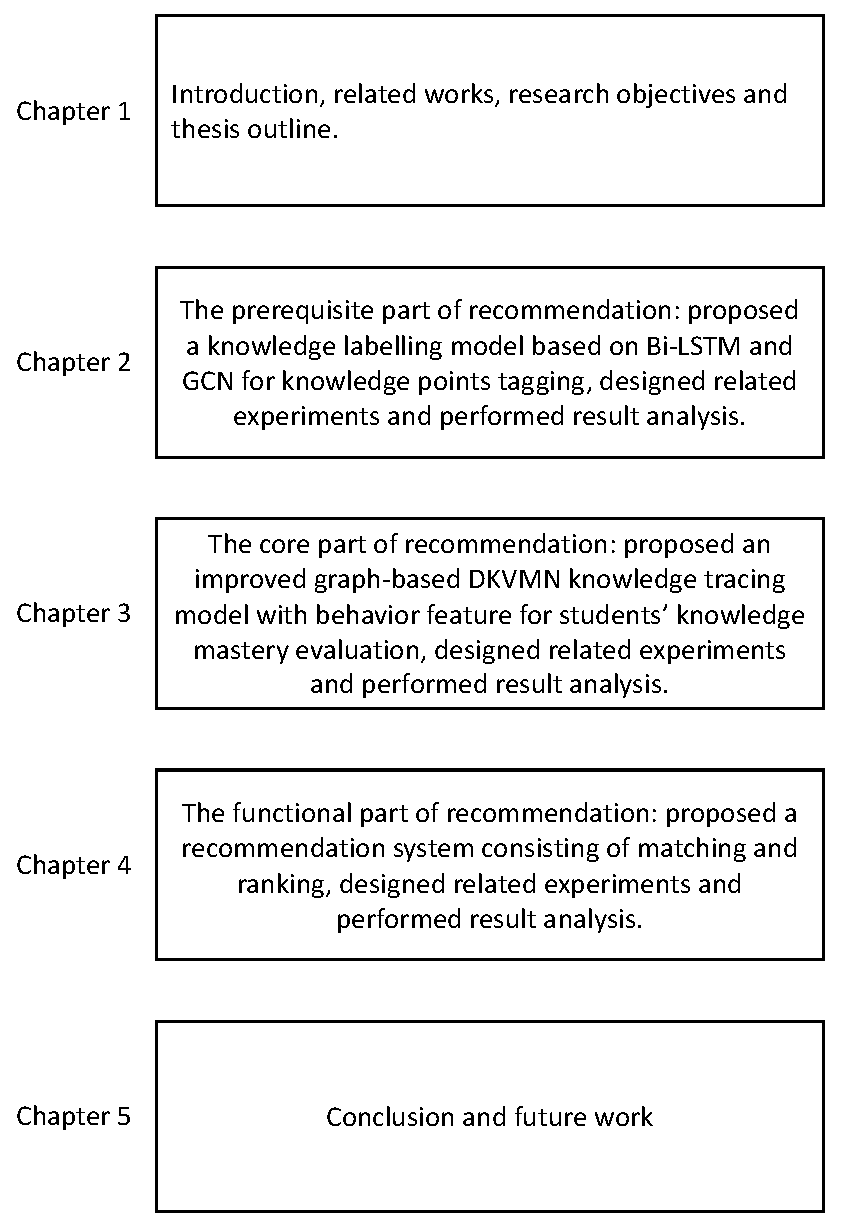
\includegraphics[width=0.75\textwidth]{ch1-architecture.pdf}
    \caption{The structure of the thesis.}\label{fig:ch1-ov}
\end{figure}



% \nomenclature[z-DEM]{DEM}{Discrete Element Method}
% \nomenclature[z-FEM]{FEM}{Finite Element Method}
% \nomenclature[z-PFEM]{PFEM}{Particle Finite Element Method}
% \nomenclature[z-FVM]{FVM}{Finite Volume Method}
% \nomenclature[z-BEM]{BEM}{Boundary Element Method}
% \nomenclature[z-MPM]{MPM}{Material Point Method}
% \nomenclature[z-LBM]{LBM}{Lattice Boltzmann Method}
% \nomenclature[z-MRT]{MRT}{Multi-Relaxation
% 	Time}
% \nomenclature[z-RVE]{RVE}{Representative Elemental Volume}
% \nomenclature[z-GPU]{GPU}{Graphics Processing Unit}
% \nomenclature[z-SH]{SH}{Savage Hutter}
% \nomenclature[z-CFD]{CFD}{Computational Fluid Dynamics}
% \nomenclature[z-LES]{LES}{Large Eddy Simulation}
% \nomenclature[z-FLOP]{FLOP}{Floating Point Operations}
% \nomenclature[z-ALU]{ALU}{Arithmetic Logic Unit}
% \nomenclature[z-FPU]{FPU}{Floating Point Unit} 
% \nomenclature[z-SM]{SM}{Streaming Multiprocessors}
% \nomenclature[z-PCI]{PCI}{Peripheral Component Interconnect}
% \nomenclature[z-CK]{CK}{Carman - Kozeny}
% \nomenclature[z-CD]{CD}{Contact Dynamics}
% \nomenclature[z-DNS]{DNS}{Direct Numerical Simulation}
% \nomenclature[z-EFG]{EFG}{Element-Free Galerkin}
% \nomenclature[z-PIC]{PIC}{Particle-in-cell}
% \nomenclature[z-USF]{USF}{Update Stress First}
% \nomenclature[z-USL]{USL}{Update Stress Last}
% \nomenclature[s-crit]{crit}{Critical state}
% \nomenclature[z-DKT]{DKT}{Draft Kiss Tumble}
% \nomenclature[z-PPC]{PPC}{Particles per cell}

%*******************************************************************************
%****************************** Second Chapter *********************************
%*******************************************************************************

\chapter{Exercise Knowledge Point Mining Based on Graph Neural Network}

\ifpdf
    \graphicspath{{Chapter2/Figs/Raster/}{Chapter2/Figs/PDF/}{Chapter2/Figs/}}
\else
    \graphicspath{{Chapter2/Figs/Vector/}{Chapter2/Figs/PDF/}{Chapter2/Figs/}}
\fi


\section{Research Motivation}
%在推荐系统的各环节,包括数据收集、数据挖掘和数据推荐,都以建立高质量的数据集作为基础。对于本文的研究主题习题推荐系统而言,建立一个规范的习题库对于建立一个试题推荐系统是重要的第一步。题库建设也是一项十分复杂而困难的工作,需要综合考虑习题数据的各个层面,为习题添加足够多的附加信息用于后续的数据挖掘。高中数学具有数百个知识点,平均每个知识点有从易到难的不同难度梯度的数十道习题。一个优质数学学科题库的规模为十万规模。除去数量上的要求,优质题库除了题目质量,以及对教育内容(教材)的匹配度之外,还有两个根本性问题,其一为知识点关系网络构建,其二为知识点-习题关系构建。而就是对于这些因素的优化,导致了优质题库的建设门槛,以及极高的成本。而市面上的题库往往缺失了对于这些因素的重视,导致出现了许多质量不高的习题数据库。所以,对题目的知识点标签的标注,以及知识体系的构建,是优质题库建设过程中最为核心的问题之一。

All aspects of the recommendation system, including data collection, data mining, and data recommendation, are predicated on establishing a high-quality data source. In this thesis's study topic, establishing a standardized and structured exercise database is the critical first step to build a test recommendation system. The construction of an exercise corpus is also a complex and challenging task, requiring comprehensive consideration of all aspects of the exercise data and adding enough additional information to the exercises for subsequent data mining. High school mathematics has hundreds of knowledge points, and on average, each point has dozens of exercises of different difficulty gradients from easy to difficult. The size of a high-quality math subject exercise corpus is 100,000 scale. In addition to the quantitative requirements, there are two fundamental issues in a quality exercise corpus, in addition to the quality of the questions and the matching of the educational content (textbooks), one is the construction of the knowledge point relationship network, and the other is the construction of the knowledge point-exercise relationship.

Moreover, it is the optimization of these factors that leads to the construction threshold of high-quality exercise corpus and the extremely high cost. The question databases on the market often lack attention to these factors, leading to the emergence of many poor-quality exercise databases. Therefore, labeling the questions' knowledge points and constructing the knowledge system is one of the most central issues in building a quality exercise corpus.

%建立试题推荐系统的一个关键问题是如何结合知识点来推荐题目。在考虑这个问题的解决方案的时候,我们首先要考虑的是,我们需要什么样的知识体系和知识点标签。在教材和教学大纲中,以及各种教辅中,会有各种对``知识点''的描述。在高中数学中的知识点,如函数、定义域、值域或解析式等,有直接的概念,也有方法的应用,有专题的抽象,也有相似解法的汇总。这并没有一种标准的分类方法,知识点系统构建的方法可能是千差万别的。作为数据挖掘的任务而言,我们更关注其涉及到的概念和技能点,这些可以通过习题文本来进行隐藏信息挖掘。作为一个对学生知识掌握熟练度进行分析的习题推荐系统,那么知识点的标签应该要能够描述题目测验的核心知识点、方法或思路,要能够区分对于学生的能力要求点,这样才能构建更为强大的用户知识点掌握度模型和推荐引擎。

One of the critical problems in building a test recommendation system is recommending topics in conjunction with knowledge points. When referring to the solution to this problem, the knowledge point labels should be considered. In textbooks and syllabi and various teaching aids, there are various descriptions of ``knowledge points''. Knowledge points in high school mathematics, such as functions, definition domains, value domains, or analytic equations, have direct concepts, applications of methods, abstractions of topics, and summaries of similar solutions. There is no one standard way to classify these, and the methods of knowledge point system construction may be very different. As far as the task of data mining is concerned, this thesis is more concerned with the concepts and skill points it involves, and these can be concluded for confidential information through the text of the exercises. As an exercise recommendation system that analyzes students' knowledge mastery proficiency, the knowledge point labels should be able to describe the core knowledge points, methods, or ideas of the topic quiz and be able to distinguish the ability requirement points for students to build a more robust user knowledge mastery model and recommendation engine.
%在本章中,挖掘的知识点标签,是用于题目的推荐和分析报告。它要求完善题目的知识点关联,即对题目打上若干对应的知识点标签,其中知识点之间也会存在依赖关系,另外就是要建立完整的知识点知识图谱用于生成学生的学习报告。对于第一个问题,它实际上是用题目文本来进行知识点挖掘的任务,也是一个分类任务。具体一点而言,主要是依据题目短文本信息进行层次化分类的任务。在这个任务中,我们需要使用到最基础的技术是自然语言处理和机器学习。也即,通过对大量人工标注好的题目文本和知识点标签结果(也称为训练语料)的学习——通过自然语言处理的技术获取题目文本的特征,通过机器学习来得到分类模型——从而使得系统具有了自动做知识点分类的能力。在这个定义中,待分类对象为题目(包括题干、答案、解析等等),分类结果是一组知识点标签。学习系统的输入就是一组训练习题,即\(n\)道已经标注好的题目及其对应的知识点标签;学习系统依据训练数据,训练给定的分类模型。在预测阶段,输入待标注的习题,输出一组对习题知识点的预测标注结果。

\section{Research Contribution}
In this chapter, a multi-knowledge point labeling classification method for exercises is proposed. The method is divided into two parts: textual information characterization using Attentional bidirectional LSTM and multi-knowledge point labeling classifier generation using GCN embedding learning method, and finally the classifier is used to perform knowledge point labeling task on the exercises. The knowledge point labels are mined for topic recommendation and analysis reports. It requires refining the knowledge point association of the topic, i.e., several corresponding knowledge point tags for the topic, where there will also be dependencies between the knowledge points and build a complete knowledge map of knowledge points for generating student learning reports. The first problem is a knowledge point mining task using the topic text, which is also a classification task. To be more specific, it is a hierarchical classification task based on the topic's short text information. The most basic natural language processing (NLP) technologies and machine learning should be used in this task. By learning a large amount of manually labeled topic text and knowledge point labeling results (also called training corpus) - obtaining the features of the topic text through NLP techniques and obtaining the classification model through machine learning. The system can do knowledge point classification automatically. In this definition, the object to be classified is a topic (including stem, answer, paraphrase, etc.), and the result is a set of knowledge point labels. The input to the learning system is a set of training exercises, i.e., \(n\) questions that have been labeled with their corresponding knowledge labels; the learning system trains the given classification model based on the training data. In the prediction phase, the exercises' input to be labeled is used to output a set of predicted labeling results for the exercises' knowledge points.

\section{Proposed Model}
%在本节中,提出了一个基于图神经网络的模型用于进行试题-知识点关联和知识点知识图谱的建立。该模型大致分为两个部分,第一个部分用一个基于图卷积神经网络半监督学习和文本挖掘嵌入学习的算法来实现的试题-知识点关联模块,用于实现试题知识点标注和关联。第二部分考虑到高中数学的知识的体系化,结合先验领域知识,用改进的R-GCN算法来构建高中数学知识点知识图谱。

% In this section, a graph neural network-based model is proposed for test question-knowledge point association and knowledge mapping of knowledge points. The architecture has two segments. The first one is an exercise-knowledge point association module implemented with a semi-supervised learning algorithm based on GCNs and text mining embedding learning for test knowledge point labeling and association. The second part considers the systematization of high school mathematics knowledge and combines a priori domain knowledge with an improved R-GCN algorithm to construct a knowledge graph of high school mathematics knowledge points.

\subsection{Algorithm Overview}
%本节的任务是构造一个挖掘习题-知识点关系的模型和一个挖掘知识点之间关联的模型。建立习题-知识点关系即对习题进行知识点标注,习题的知识点是理解习题和求解习题所用到的知识概念的集合。所以准确描述一道试题的知识点,对于后续的知识追踪和推荐过程十分重要。目前已经存在的基础分类方式有专家标注和机器学习两种方式。前者即教育专家结合自己的专业知识对试题进行知识点标注,但当题量或题目复杂度较高时,人工标注存在工作量大,主观度高和标注不完善等问题。另外考虑到知识点之间的关联,人工标注也存在无法考虑到知识内联关系。另一种方式则是用基于规则的自动化标注的方法,它通过文本模式匹配等非智能方式来进行知识点关键词匹配。但有许多习题往往并不具有显式的知识点文本,因此该方法的正确率不够理想。此外,一个习题往往具有多个知识点,因此实际上知识点挖掘是一个多标签分类问题~\cite{tsoumakas2007multi,zhang2013review,liu2020emerging}。本章也会对``如何有效建模知识点间的关系''来进行讨论并提出一种基于图神经网络的多标签分类模型。

This section aims to construct a model for mining the exercise-knowledge point relationship and mining the association between knowledge points. Establishing an exercise-knowledge point relationship means labeling the knowledge points of an exercise and collecting knowledge concepts to understand and solve the exercise. Therefore, accurately describing a test question's knowledge points is essential for the subsequent knowledge tracking and recommendation process. The two basic classification approaches that already exist are expert labeling and machine learning. The former means that education experts combine their professional knowledge to label knowledge points of test questions. However, when the number of questions or complexity of questions is high, the manual labeling has problems such as high workload, high subjectivity, and imperfect labeling. Also, considering the association between knowledge points, the manual labeling has the problem of not taking into account the inline knowledge relationship. Another way is to use the rule-based automated labeling method, which performs knowledge keyword matching by non-intelligent means such as text pattern matching. However, many exercises often do not have explicit knowledge point texts, so this correctness rate is not satisfactory. Also, an exercise often has multiple knowledge points, so in effect, knowledge point mining is a multi-label classification problem~\cite{tsoumakas2007multi,zhang2013review,liu2020emerging}. This chapter also discusses ``how to effectively model the relationships between knowledge points'' and proposes a multi-label classification model based on graph neural networks.


%在2019年,提出了一种多标签图像分类模型,受该模型启发,本章提出了一个基于注意力机制习题文本特征提取和基于图神经网络知识点关系挖掘的多知识点标注模型,它通过数据驱动的方式建立知识点关系图描述知识点间的关联关系,对知识点分别建立分类器,然后对习题的文本特征进行多标签分类。其主要架构图如下。

In 2019, a multi-label image classification model was proposed~\cite{chen2019multi}. Inspired by this model, this chapter proposes a multi-knowledge point labeling model based on attention mechanism exercise description text feature extraction and graph convolutional neural network (GCN) based knowledge point relationship mining, which builds a knowledge point relationship graph to describe the association relationship between knowledge points by a data-driven approach, builds classifiers for knowledge points separately, and then performs multi-label classification. Its main architecture diagram is shown in \figname{\ref{fig:ch2-modelarchitecture}}.

\begin{figure}[htbp!]
    \centering
    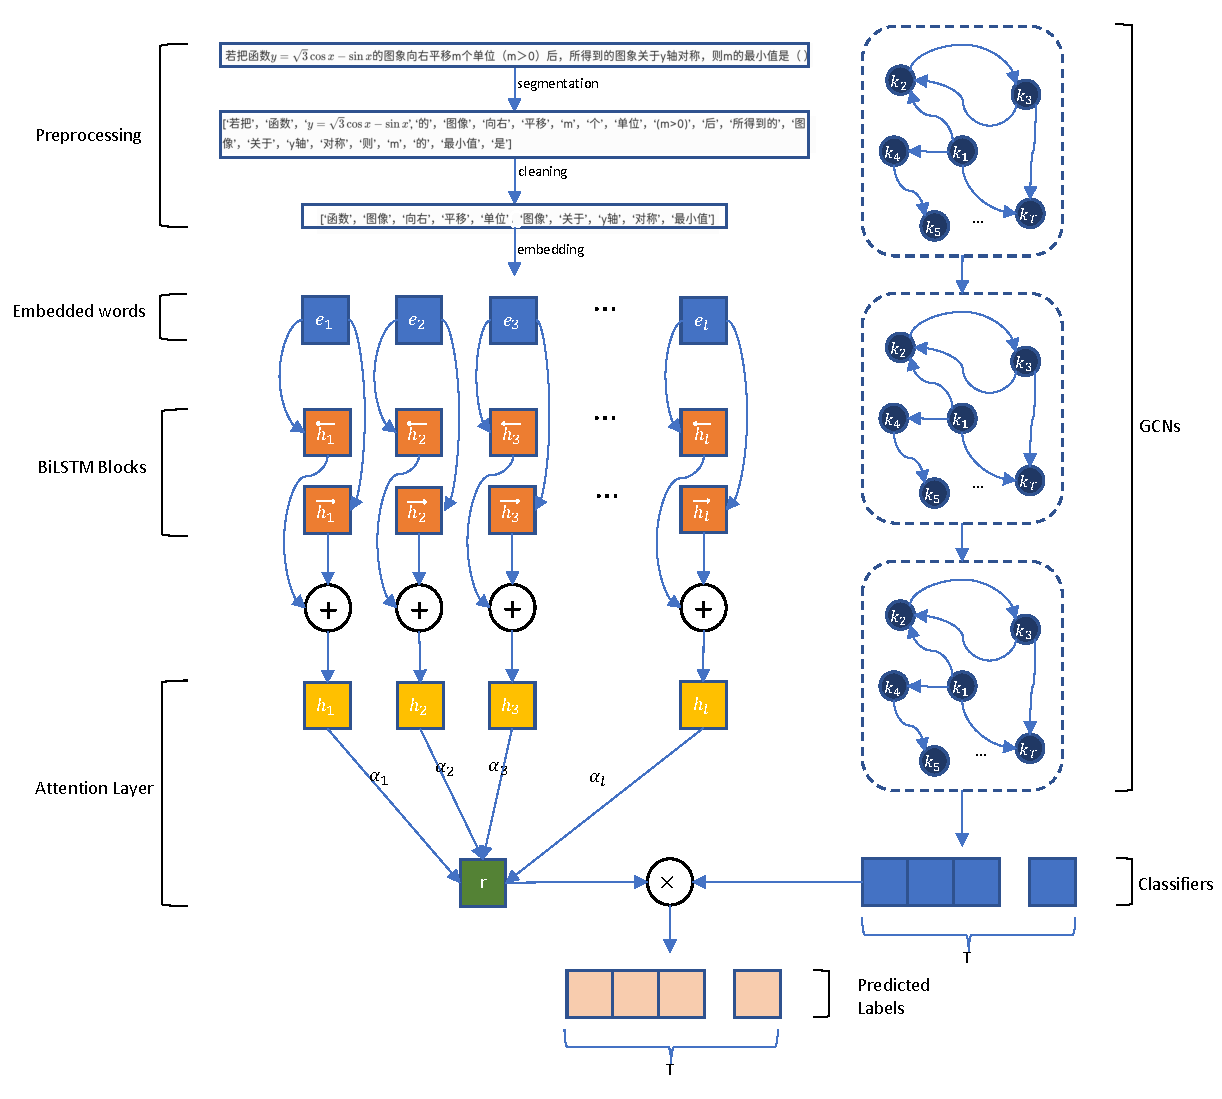
\includegraphics[width=1.0\textwidth]{ch2-model-architecture.pdf}
    \caption{Structure of the knowledge labeling model}\label{fig:ch2-modelarchitecture}
\end{figure}

%从结构上我们可以看到,模型中一般有两部分,其中

%第一部分是习题文本挖掘模块 ,它用自然语言处理技术来对题目(包括问题描述和答案)进行文本挖掘,它包含隐藏的知识点信息。本文设计了一个端到端的网络训练方式,实现模型整体的迭代学习。具体而言,它包括进行文本分词、过滤和去重登部分的文本预处理部分,进行词向量embedding计算的embedding层和进行文本信息挖掘的基于Attention的双向LSTM网络,该网络由Peng等人于2016年提出~\cite{zhou2016attention},输出一个对于习题文本的向量表示。

%第二部分是基于图卷积神经网络的知识点关联多标签分类器,它将知识点映射到一组相互依赖的目标分类器。这些分类器与第一部分输出的习题信息表征向量进行计算,输出一个代表各个知识点标注概率的结果向量。

From the structure, it can be seen that there are generally two parts to the model:
\begin{enumerate}
    \item The first part is the exercise description text information mining module, which uses a Bi-LSTM network with an added attention mechanism to text-mine hidden knowledge information on questions (including question descriptions and answers). In this thesis, an end-to-end network training approach is designed to achieve the model's overall iterative learning. Specifically, it consists of a text preprocessing part that performs the text subdivision, filtering, and deduplication parts, an embedding layer that performs the word vector embedding calculation, and an Attention-based Bi-LSTM (Bi-LSTM) network that performs text information mining, which was proposed by Peng et al.\ in 2016~\cite{zhou2016attention}, outputting a textual information representation vector.
    \item The second part is a GCN-based knowledge point association multi-label classifier, which maps knowledge points to a set of interdependent target classifiers. These classifiers are computed with the exercise information representation vector outputted by the first part to output a result vector representing each knowledge point's labeling probability.
\end{enumerate}


\subsection{The Exercise Description Text Mining}
%本部分基于Peng等人提出的Attention based Bi-LSTM模型,该模型的结构如图所示\ref{}
This section is based on the Attention based Bi-LSTM, whose architecture design is shown in \figname{\ref{fig:ch2-model-bilstm}}.
\begin{figure}[htbp!]
    \centering
    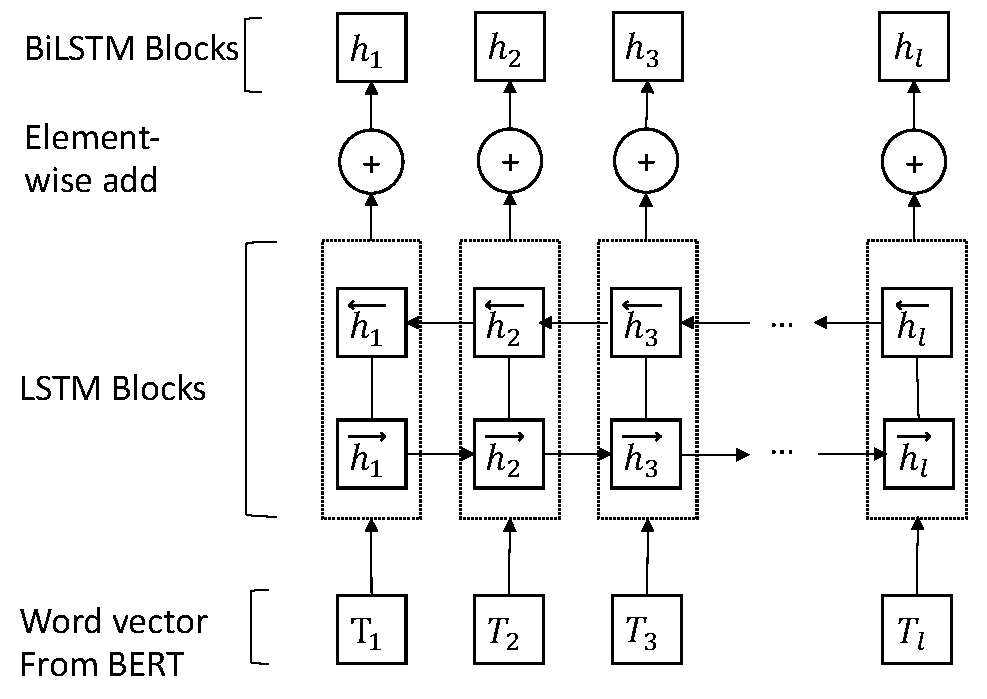
\includegraphics[width=1.0\textwidth]{ch2-model-bilstm.pdf}
    \caption{Structure of attention based Bi-LSTM}\label{fig:ch2-model-bilstm}
\end{figure}

%该模型包含4个层: 
The model includes four layers: Preprocess Layer, Embedding Layer, Bi-LSTM layer, Attention Layer, and Output Layer:
\subsubsection{Pre-process Layer}

%在预处理阶段,主要包括分词、清洗、正则化等方式。考虑到我们的研究对象为中文高中数学试题,相对于英文,中文句子中间没有中间空格,所以必须用分词算法来将句子分解为分词。内容中有很多对句意表达无关的文本,如果直接进行计算会造成大量的干扰和冗余信息,所以另外的文本清理也是必要的步骤。\figname{ref{ch2-fig3}}显示了一个预处理练习文本的例子。

% - 中文分词是中文自然语言处理的一个基本步骤,在中文中,一个句子中词与词之间没有自然分隔,因此必须先对句子进行分词操作,将句子分解为词。分词效果将直接影响词性、句法树等模块的效果。选择合适的的中文分词算法能够达到更好的自然语言处理效果,帮助计算机理解复杂的中文语言。目前,中文分词主要分为基于词典规则匹配和基于统计模型两种算法,相对于前者,后者具有更好的泛化性和学习能力,对先验规则之外的分词例如歧义词和未登录词表现更好。在本模型中,采用了目前较为热门的jieba分词器,它采用了基于汉字成词能力的 HMM 模型,能够找出基于词频的最大切分组合。用户也可以自定义停用词和用户词典来实现对于专有名词的识别。

% - 清洗:在对习题进行文本挖掘时,会遇到大量无关的文本信息,例如对于以下习题:

The preprocessing stage mainly includes word separation, cleaning, and regularization. Considering that our research object is Chinese high school mathematics test questions, compared with English, there is no middle space in the middle of sentences of Chinese language, so it is necessary to use the word separation algorithm to decompose the sentences into subwords. There are many texts in the content that are irrelevant to the sentence expression, which will cause much interference and redundant information if the calculation is performed directly, so additional text cleaning is also a necessary step. The \figname{\ref{fig:ch2-model-preprocessing}} shows an example of preprocessing of an exercise description text.

\begin{figure}[htbp!]
    \centering
    
\includegraphics[width=1.0\textwidth]{ch2-model-preprocessing.pdf}
    \caption{Example of preprocessing}\label{fig:ch2-model-preprocessing}
\end{figure}

% - 分词。相对于其他表音语言如英语、西班牙语,中文语言预处理需要额外的分词步骤。在汉语中的词与词之间不存在自然分隔,因此需要人为对句子按照词义进行分割。选择合适的汉语分词算法可以为后续的处理奠定基础,提高整体模型性能。目前,汉语分词主要分为基于词典规则匹配和基于统计模型的两种算法。与前者相比,后者具有更好的泛化能力和学习能力。它用于先验规则之外的分词,如歧义词和未注册词表现较好。在该模型中,采用了目前流行的jieba分词,实现了基于Trie书结构的词条图扫描,利用阶段规划和HMM模型等算法,找到基于词频的最大分词分组和合并,实现了未来登录词的识别。用户还可以自定义停字和用户字典,实现专有名词识别。
% - 清理。语料库清理:保留语料库中的有用数据,删除噪声数据。常见的清洗方法包括:人工重删、对齐、删除和标注。对于句子中不需要的词,即停顿词,它们的存在不影响句子的意思。在文本中,会有大量的功能词、代词或没有特定含义的动词和名词。这些词对文本分析没有帮助,所以这些停顿词可以去掉。对于习题文本,有很多数学表达式、符号等,考虑到很多习题中的这些表达式不是文本格式,必须采用OCR技术将数学表达式从图片预处理成文本。因此,在中文文本足够的情况下,可以考虑将数学表达式过滤掉,以减少计算负荷。

\begin{itemize}
    \item Segmentation: Compared to other phonetic languages such as English and Spanish, Chinese language preprocessing requires an extra step of word separation.  There is no natural separation between words in Chinese sentences. Therefore artificial segmentation of sentences according to word meanings is required. Choosing a suitable Chinese word segmentation algorithm can lay the foundation for the subsequent processing and improve the overall model performance. At present, the Chinese word segmentation is mainly divided into two types of algorithms: rule-based lexical matching and statistical model-based. Compared with the former, the latter has better generalization ability and learning ability. It performs better for word separation beyond the a priori rules, such as ambiguous words and unregistered words. In this model, the currently popular jieba subword is used to implement a word graph scan based on the Trie book structure, and algorithms such as stage planning and HMM model are used to find the maximum subword grouping and merging based on word frequency to achieve the identification of future logged-in words. Users can also customize stop words and user dictionaries from achieving proper noun recognition.
    \item Cleaning: Corpus cleaning preserves useful data in the corpus and deletes noisy data. Common cleaning methods include manual deduplication, alignment, deletion, and labeling. For words that are not necessary for a sentence, i.e., stop words, their existence does not affect the sentence's meaning. There will be a large number of function words, pronouns, or verbs and nouns with no specific meaning in the text. These words are not helpful to the text analysis so that these stop words can be removed. For the exercise description text, there are many mathematical expressions, symbols, etc. Considering that these expressions in many exercises are not in text format, OCR technology must be applied to preprocess mathematical expressions from pictures to text. Therefore, when the Chinese text is sufficient, mathematical expressions can be removed to reduce the calculation load.
\end{itemize}

%经过数据处理的步骤,得到了一个干净的文本token序列,接下来在Embedding层可以利用BERT技术来进行文本embedding操作。
After the data processing step, a clean sequence of text tokens is obtained, and next in the Embedding layer, the BERT technique can be used to perform text embedding operations.

\subsubsection{BERT-Based Embedding Layer}
%在深度学习的应用过程中,嵌入是一种将符号形式的自然对象、模式等转化为数学空间中的向量的方法,是一种从离散空间到连续空间的转换,为神经网络在各方面的应用带来了极大的扩展。嵌入是一个将离散变量转为连续向量表示的一个方式。在神经网络中,embedding 是非常有用的,因为它不光可以减少离散变量的空间维数,同时还可以有意义的表示该变量。在词嵌入学习的研究中,有one-hot、Word2Vec和BERT等常见的词嵌入学习算法和模型。one-hot编码是最朴素的方法,它将所有的词语二进制化,即所有的词语只有存在或不存在两种情况,因此每个词语都是一个只有一个1其他全是0的二进制向量。当词语量较大时,该向量的长度也会相当长,在后续的计算也会产生大量的无效计算,即稀疏矩阵计算问题。Word2Vec由Google语2013年提出~\cite{church2017word2vec},它通过词语来预测它的上下文或者通过上下文来预测词语,是一种静态的词嵌入学习模式,但在解决多义词等问题上遇到瓶颈。Google于2018年提出的Bidirectional Encoder Representations from Transformers(BERT)模型利用Transformer作为基本单元,预训练masked语言模型,在几乎所有的自然语言处理任务都取得了State of the art(SOTA)的性能表现。它具有极强的语义表征效果。本文利用BERT来作为词Embedding向量学习模块,能更好地在不同习题文本的不同语境中取得更好的泛化和自适应能力。

In applying deep learning, embedding as a preprocessing approach for generating embedded vectors brings a great extension to neural networks' application in various aspects.  In applying deep learning techniques, embedding is an instrumental skill because it reduces the spatial dimensionality of a discrete variable and allows a meaningful representation of that variable. For example, in NLP, if basic one-hot coding is used, it often results in too many dimensional and sparse vectors and also fails to learn the dependencies between vectors. The embedded vectors are updated during embedding training, which can clearly show the exercises between the vectors. The one-hot encoding is the most naive method, which turns all words into binary patterns, i.e., all words are only present or absent in two cases, so each word is a binary vector with only 1-value and all other 0-values. When the amount of words is large, this vector's length will also be quite long, and the subsequent computation will also generate a large number of invalid computations, i.e., the sparse matrix computation problem. Word2vec was proposed by Google Language 2013~\cite{church2017word2vec}, which predicts its context by words or predicts words by contexts, a static word embedding learning model, but encounters bottlenecks in solving problems such as polysemous words. The Bidirectional Encoder Representations from Transformers (BERT) model proposed by Google in 2018 utilizes the Transformer as the base unit to pre-train masked language models, achieving State of The Art (SOTA) performance in almost all NLP tasks. It has a powerful semantic representation effect. In this thesis, BERT is utilized as a word embedding vector learning module to achieve greater generalization and adaptive capabilities in different contexts of different idiomatic texts.

%在习题文本中,会出现一些组合词,即由多个词组合而成的具有不可分割词义的词组,由于在BERT的训练样本生成阶段,会对词进行mask操作,因此这些组合词有可能会被分别mask。导致出现歧义,引起训练性能退化。因此,本文应用全词mask的处理方式,该方法由cui等人于2019年提出~\cite{cui2019pre}。通过应用全词mask,当一个组合词的一个部分被mask,则该组合词的其他部分也会被mask。如图所示。


In the exercise description text, there will be some combinations of words, i.e., groups of words with indivisible lexical meanings formed by combining multiple words. Since the words are masked during the BERT training sample generation phase, these combinations may be masked separately, resulting in ambiguity and causing training performance degradation. Therefore, this thesis applies Whole Word Mask processing (WWM), proposed by Cui et al.\ in 2019~\cite{cui2019pre}. By applying WWM, when one part of a combined word is masked, then the other parts of that combined word are also masked, as shown in \figname{\ref{fig:ch2-bert-wwm}}.

\begin{figure}[htbp!]
    \centering
    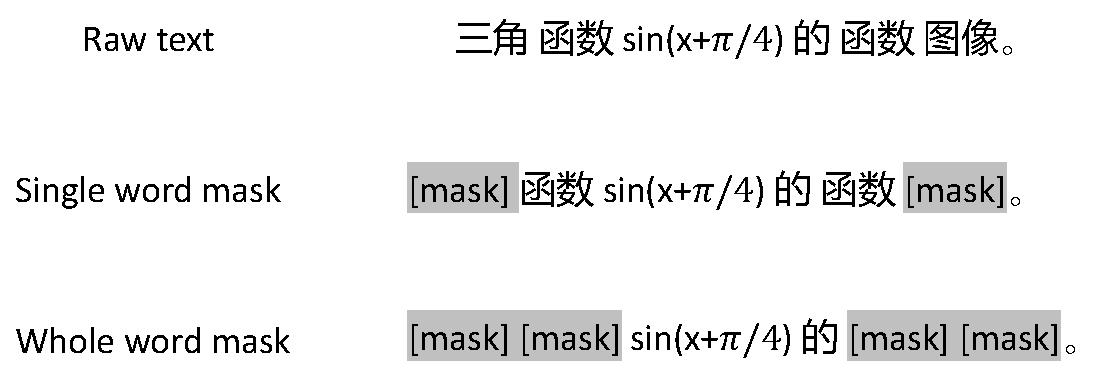
\includegraphics[width=1.0\textwidth]{ch2-bert-wwm.pdf}
    \caption{Whole word mask}\label{fig:ch2-bert-wwm}
\end{figure}

%将经过分词处理得到的习题文本词原始序列的部分词进行WWM处理,在序列的开头添加标记[CLS],句子间用[SEP]分隔符标示。经过训练,输出词embedding向量。每个词的输出embedding由三个部分组成,即token embedding、segment embedding和position embedding,它们从不同的角度对词进行嵌入信息表征。随后,将词嵌入向量输入BERT的特征提取双向Transformer层,可以获得包含深度语义特征的特征序列表征向量。整体架构如图所示。

WWM processes some words of the original sequence of exercise description text words obtained after the word separation process, and the marker [CLS] is added at the beginning of the sequence, and the inter-sentence is marked by [SEP] separator. After training, the word embedding vector is output. Each word's output embedding consists of three parts: token embedding, segment embedding, and position embedding, which characterize the word's embedding information from different perspectives. Subsequently, the word embedding vector is fed into the feature extraction bidirectional Transformer layer of BERT, and the feature sequence representation vector containing deep semantic features can be obtained. The overall architecture is shown in the \figname{\ref{fig:ch2-bert-model}}.

\begin{figure}[htbp!]
    \centering
    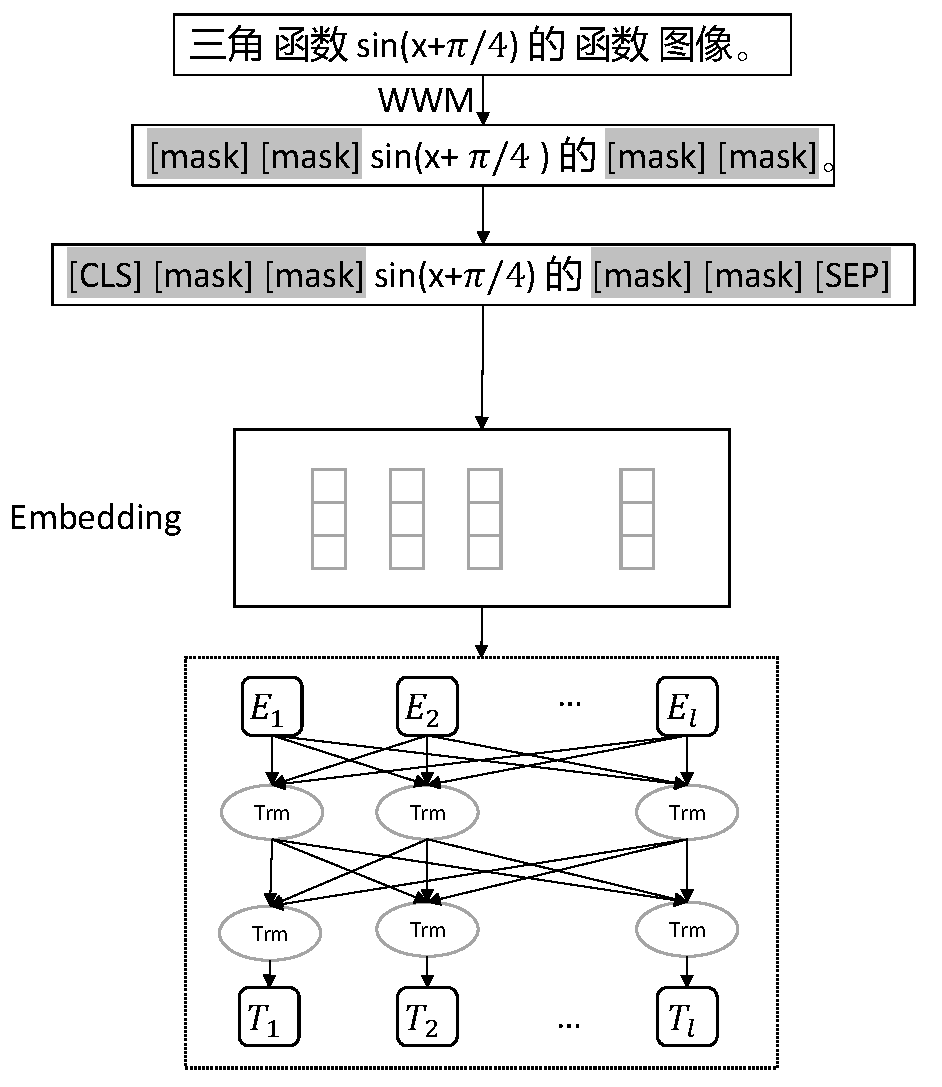
\includegraphics[width=1.0\textwidth]{ch2-bert-model.pdf}
    \caption{BERT-based embedding}\label{fig:ch2-bert-model}
\end{figure}

\subsubsection{Bidirectional LSTM Layer}
%在解决序列化模式数据建模方面,RNN具有良好的解决能力。在本节中,任务核心是一个序列到序列(Seq2Seq)的任务,输入一个题目描述的embedding向量,输出一个包含当前训练到的信息序列。最朴素的想法就是用原始的RNN,其结构如图所示,图中\(x_t\),\(h_t\)和\(y_t\)分别表示在时间t的输入值、隐藏值和输出值。

RNNs are well equipped to solve various types of problems and tasks in serialized pattern data modeling. In this section, the core of the task is a sequence-to-sequence (Seq2Seq) task, where an embedding vector described by the topic is input and a sequence containing the currently trained information is output. The most rudimentary idea is to use the original RNN.\@ Its structure is shown in the \figname{\ref{fig:ch2-rnn-model}}, where \(x_t\), \(h_t\) and \(y_t\) denote the input, hidden and output values at time \(t\), respectively. Then, the RNN training formula can be written as~\eqname{\ref{fml:rnn-train}}:

\begin{align}\label{fml:rnn-train}
    \begin{split}
        h^{t+1} & =f(W^h_{t} h^t+W^i x^t) \\
        y^{t+1} & =f(W^o h^{t+1})
    \end{split}
\end{align}


\begin{figure}[htbp!]
    \centering
    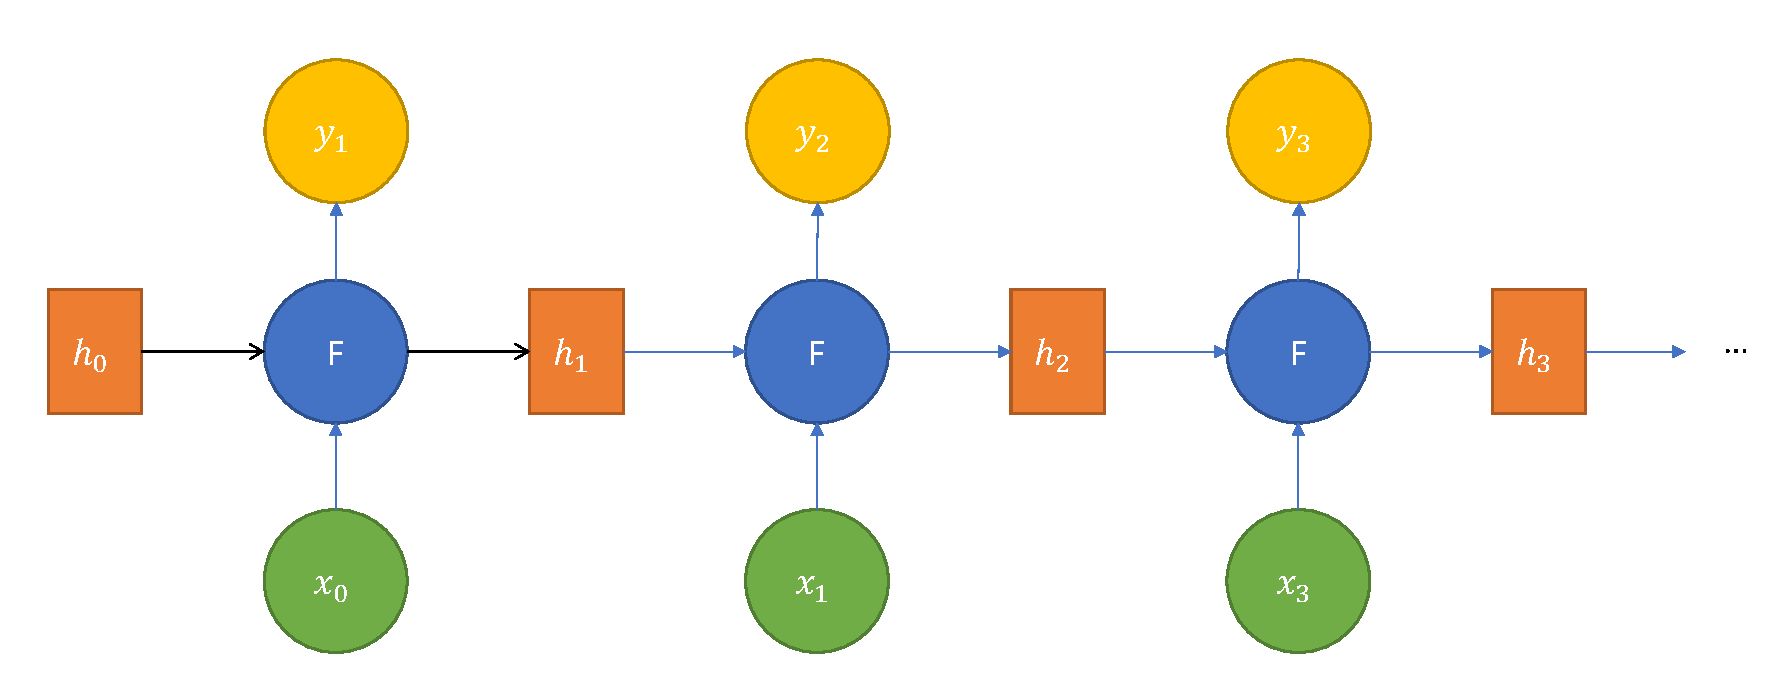
\includegraphics[width=1.0\textwidth]{ch2-rnn-model.pdf}
    \caption{Naive RNN unit}\label{fig:ch2-rnn-model}
\end{figure}

%但是,当序列较长时,就会出现长依赖性的问题。例如,对于一个序列,当前的状态依赖于离当前状态很远的一个状态,随着时间间隔的增加,RNNs学习这个状态的能力会大大降低。LSTM是作为针对RNN的这种缺陷的一种解决方案被提出来,它运用门控机制来实现长期记忆。解决RNN的梯度爆炸或梯度消失等问题。在捕捉序列信息方面也具有良好的性能。其结构如图所示,表示\(t\)时刻的一个LSTM单元内的计算细节。其中,\(\sigma\)为激活函数,\(c_t\)为单元状态表征,\(f_t\)为遗忘门控计算,\(i_t\)为输入门控计算,\(o_t\)为输出门控计算,\(h_t\)为隐藏状态表征。通过由门控控制的遗忘机制,可以有效建模对于远距离序列单元信息。

However, when the sequence is long, the problem of long dependencies arises. For example, for a sequence, the current state depends on a state far away from the current state, and as the time interval increases, the ability of RNNs to learn state representation is greatly reduced. Long short-term memory (LSTM)~\cite{lstm1997}, as a solution to overcome shortcomings of RNN, which uses a gating mechanism to achieve long-term memory. It solves the problems such as gradient explosion or gradient disappearance of RNN. It also has a good performance in capturing sequence information. The general model of LSTM is like \figname{\ref{fig:ch2-lstm-model}}, which represents the computational details within an LSTM cell at the moment of \(t\). Among them, \(\sigma\) is the activation function, \(c_t\) is the cell state representation, \(f_t\) is the forgetting gating calculation, \(i_t\) is the input gating calculation, \(o_t\) is the output gating calculation, and \(h_t\) is the hidden state representation. The forgetting mechanism controlled by gating can be effectively modeled for long-range sequential unitary information.

\begin{figure}[htbp!]
    \centering
    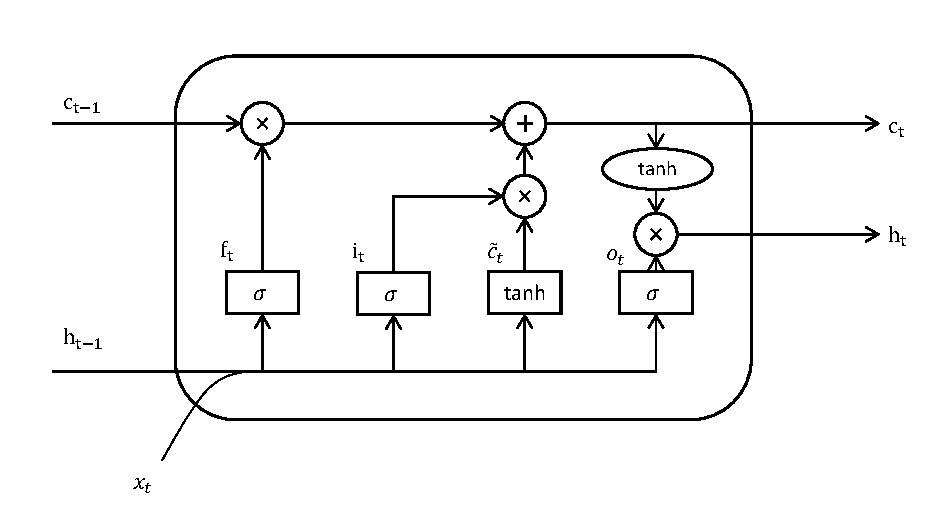
\includegraphics[width=1.0\textwidth]{ch2-lstm-model.pdf}
    %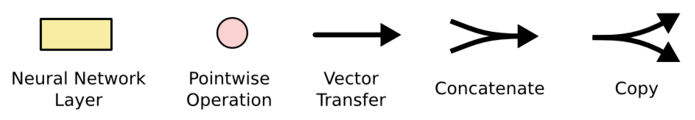
\includegraphics[width=1.0\textwidth]{ch2-fig8.png}
    \caption{Structure of LSTM unit}\label{fig:ch2-lstm-model}
\end{figure}

%单向LSTM也有一个固有的缺陷,它只能捕获\(t\)时刻以前的序列状态信息,即只能捕获之前序列输入。双向LSTM通过将反向序列输入LSTM并与正向LSTM序列进行聚合,可以捕获双向的语义信息,同时对双向的依赖建模。
One-way LSTM also has an inherent drawback that it can only capture the sequence state information before \(t\) moment, i.e., it can only capture the previous sequence input. The bidirectional LSTM (Bi-LSTM)~\cite{graves2005framewise} can capture semantic information in both directions by feeding the reverse sequence into the LSTM and aggregating it with the forward LSTM sequence, while modeling the dependencies in both directions. The Bi-LSTM output can be obtained by inputting the positive sequence and the reverse sequence input sequence into two sets of LSTM networks and perform element-wise addition. The output of positive-order LSTM is \(\overrightarrow{h_t}\), the output of reverse-order LSTM is \(\overleftarrow{h_t}\), \(\bigoplus \) means sequence concatenation. The output of Bi-LSTM is:
\begin{align}
    \begin{split}
        \overrightarrow{h_t} & = \overrightarrow{LSTM}(e_t)                       \\
        \overleftarrow{h_t}  & = \overleftarrow{LSTM}(e_t)                        \\
        h_t                  & =\overrightarrow{h_t}\bigoplus \overleftarrow{h_t}
    \end{split}
\end{align}
The Bi-LSTM Structure is like \figname{\ref{fig:ch2-model-bilstm}}.

\begin{figure}[htbp!]
    \centering
    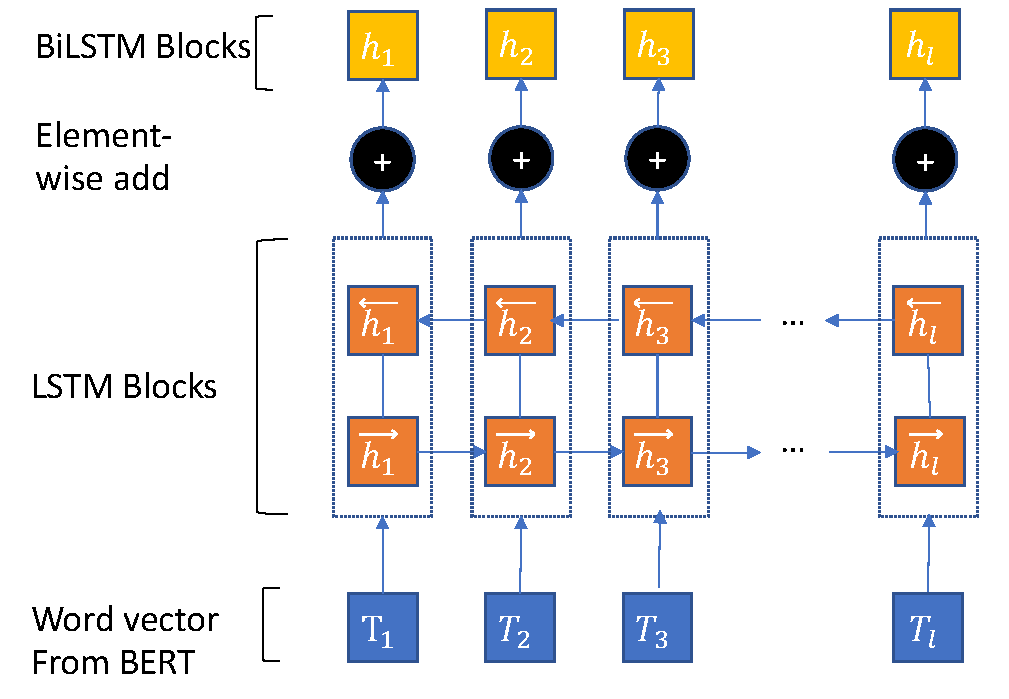
\includegraphics[width=1.0\textwidth]{ch2-bilstm-model.pdf}
    \caption{Structure of Bi-LSTM}\label{fig:ch2-model-bilstm}
\end{figure}

Here, the Bi-LSTM output a bidirectional sequence as the concatenation of positive-order and reverse-order LSTM output sequence.



\subsubsection{Attention Layer}

%由于文本挖掘任务中,每个特征词对于总体语义的影响是非对称的,即关键词在决定整个文本的含义方面有决定性的作用。Bahdanau等人提出的~\cite{bahdanau2014neural}提出了Attention机制模型正是基于这一原理。人的注意力是一种聚焦于关键信息忽略非关键信息的机制,即各个信息点的权重不一样。

%按照注意方法,编码器使用Bi-LSTM并获得隐藏状态向量 \(h_t = \ overrightarrow {h_t}) \ bigoplus \ overleftarrow {h_t} \)。在解码器阶段,计算每个编码器隐藏层状态和解码器隐藏层状态之间的相关性,并执行softmax归一化操作以获得每个隐藏层矢量的权重。将\(H\)设置为\(H = [h_1,h_2,...,h_l] \)  的隐藏状态矩阵,我们可以计算嵌入\(r\)的练习文本。计算公式如下:


Since each feature word's impact on the overall semantics in a text mining task is asymmetric, i.e., keywords have a decisive role in determining the meaning of the entire text. The proposed Attention model proposed by Bahdanau et al. is based on~\cite{bahdanau2014neural}. Human attention is a mechanism that focuses on key information ignoring non-key information, i.e., individual information points are weighted differently. This method achieved remarkable results in different tasks such as image vision~\cite{fu2017look,sun2018multi}, language mining~\cite{hu2019introductory}, and voice recognition~\cite{chorowski2015attention} and is applied widely.


Human attention is a mechanism for quickly screening high-value information from massive information. The human attention mechanism inspires the deep learning attention mechanism. This method is widely used in various types of deep learning tasks such as NLP~\cite{hu2019introductory}, image classification~\cite{fu2017look,sun2018multi}, and speech recognition~\cite{chorowski2015attention}, and has achieved remarkable results.

\begin{figure}[htbp!]
    \centering
    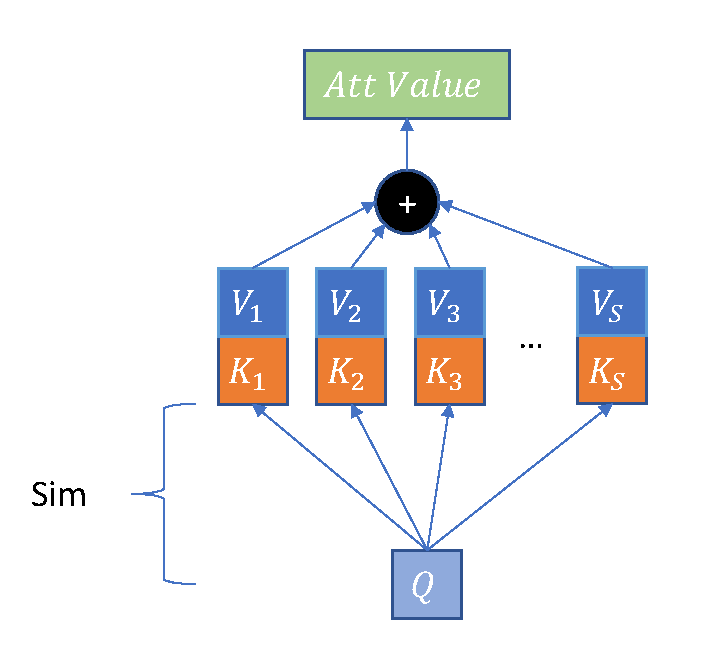
\includegraphics[width=0.7\textwidth]{ch2-model-attmodel.pdf}
    \caption{The essential idea of attention mechanism}\label{fig:ch2-model-attmodel}
\end{figure}


The essence of the attention mechanism is a group of key-value pairs \(<K, V>\) contained in Source \(S\), given an element of Query \(Q\), which is followed by calculating the \(Q\) similarity to each \(K\) and remembering the weight coefficients of the corresponding values \(V\). It is showed in \figname{\ref{fig:ch2-model-attmodel}}. Then a weighted sum is performed to obtain the final Attention value. It can be expressed as \eqname{\ref{fml:ch2-attention}}, where \(Att\) and \(Sim\) represent attention and similarity.
\begin{align}\label{fml:ch2-attention}
    Att(Q,S) = \sum_{i=1}^{|S|}Sim(Q,K_i)*V_i
\end{align}

%本节的注意力机制的核心原理是计算出对句义影响最大的词,即关键语义词,它们在之后被汇总成为句义表征向量。
Following the attention method, the encoder use Bi-LSTM and get hidden state vector \(h_t=\overrightarrow{h_t}\bigoplus \overleftarrow{h_t}\). A word attention mechanism is introduced here. The core principle of the attention mechanism in this section is to compute the words that have the greatest influence on sentence meaning, i.e., the key semantic words, which are later aggregated into a vector of sentence meaning representations. The formula is \eqname{\ref{fml:ch2-att2}}, where \(u_t\) is the hidden representation of \(h_t\), \(r\) is the output text vector, and the \(u_\omega \) is the similarity of the text vector of word aspect. By measuring the similarity between \(u_t\) and \(u_\omega \) as the importance of the word, and using the softmax function to calculate normalization and to obtain the importance weight \(\alpha_{t}\). Finally, the entire text is transformed to word representation based on semantic contribution weights.

%
After that, the entire text is represented as a weighted sum of word vectors. The context vector \(u_\omega \) can be regarded as a high-level representation of the fixed query ``what is the word conveying information'' and is randomly initialized as a learnable parameter in training.


\begin{align}\label{fml:ch2-att2}
    \begin{split}
        u_t      & = \tanh(W_\omega h_t + b_\omega )                                                    \\
        \alpha_t & =Softmax(u_t^T u_\omega) = \frac{\exp( u_t^T u_\omega)}{\sum_t \exp(u_t^T u_\omega)} \\
        r        & = \sum_t{\alpha_t h_t}
    \end{split}
\end{align}

\subsection{The GCN-based Knowledge Point Classifier Generator}
%在高中数学学科中,知识点之间具有较为复杂的相互关联例如相关、从属、包含、前驱、后继等等。这些复杂的相互关系在欧式空间往往难以建模,或这产生数据稀疏性的问题。而通过图数据结构来建立知识点间的关系则更加直观和拥有更好的解释性。回顾本模型的任务,它给出习题的描述、答案,部分已经标记好知识点,利用这些信息来对为标注知识点的习题进行知识点标注。考虑到知识点之间的依赖关系,一些在浅层特征上无法表征的深层隐藏知识点也可以通过图神经网络输出分类器被正确标注。在本模型中,用到了图卷积神经网络来建模知识点关系图,每个知识点都对应图上的一个节点。经过多个图卷积计算,生成一系列的分类器,这些分类器分别作用在文本挖掘模块产生的文本向量,每个分类器输出一个值表征该知识点与是该习题相关联的概率。其总体架构如图所示。

%本模型采用GCN结构的原因在于,GCN对于各个节点的参数共享使得学习到的分类器可以保留知识关联图中的关联信息,从而隐式表示其空间语义结构。因此输出的分类器可以保留和识别隐式知识标签依赖信息。 对于知识点的依赖关系参考数据关联方法挖掘算法例如apriori算法,通过计算知识点在习题中的共现度来计算其协关系矩阵。

In high school mathematics, knowledge points have more complex interrelationships such as correlation, subordination, inclusion, predecessor, successor, etc. These complex interrelationships are often difficult to model in Euclidean space, or this creates data sparsity problems. The establishment of relationships between knowledge points through graph data structures is more intuitive and has better interpretability. Recalling this model's task, it gives descriptions and answers to exercises, some of which have already marked knowledge points, and uses this information to mark knowledge points for exercises that are labeled knowledge points. Considering the dependence between knowledge points, some deeply hidden knowledge points that cannot be represented in shallow features can also be correctly labeled by the graph neural network output classifier. In this model, a GCN is used to learn and form the knowledge point connection graph, and each knowledge point corresponds to a node on the graph. After multiple graph convolution calculations, a series of classifiers are generated. These classifiers respectively act on the text vector generated by the text mining module. Each classifier outputs a value representing the probability that the knowledge point is associated with the exercise. Its overall structure is shown in the \figname{\ref{fig:ch2-gcn-ov}}.

\begin{figure}[htbp!]
    \centering
    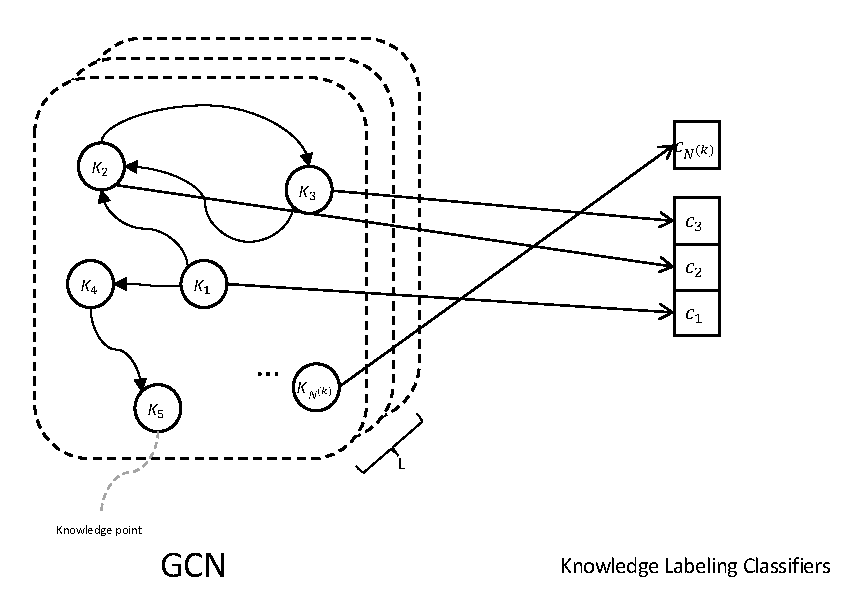
\includegraphics[width=0.8\textwidth]{ch2-gcn-ov.pdf}
    \caption{The overview of structure}\label{fig:ch2-gcn-ov}
\end{figure}



\subsubsection{Graph Convolutinal Network}
%在现实世界中,许多重要的数据集都以网络的形式产生连接,形成图状结构。一些论文对此问题进行了回顾,并试图对神经网络进行概括,并将其应用于任意图结构数据~\cite{wu2018socialgcn,dettmers2018convolutional}。图卷积神经网络(GCN)~\cite{kipf2016semi}用于处理传统卷积神经网络难以学习的非欧氏空间数据。它定义在一个图结构\(G=(V,E)\)上,其中\(V\)、\(E\)为图的顶点和边。GCN的输入为维度为\(n^v\times d^{v}\),其中\(n^v\)为节点数,\(d^v\)为各个顶点的特征维度数。此外,GCN又一个用于描述图结构的维度为\(n^v\times n^v\)的邻接矩阵\(A\)。

In the real world, many important data sets generate connections as networks that form graph-like structures. Several researchs reviewed this problem and attempted to generalize neural networks and apply them to arbitrary graph-structured data~\cite{wu2018socialgcn, dettmers2018convolutional}. The GCN~\cite{kipf2016semi} is used to process non-Euclidean spatial data that are difficult to learn by traditional convolutional neural networks. It is defined on a graph structure \(G=(V, E)\), where \(V\) is the denote of vertex and \(E\) is the denote of edge inside the graph. The input of GCN \(X = H^{(0)}\) is the first layer of GCN. The ith layer is denoted as \(H^{(i)}\), and \(H^{(i)}\in \mathbb{R}^{N^{(v)}\times d_{i}}\), where \(N^{(v)}\) is the denote of number of vertexes and \(d_{i}\) is the number of dimension of each vertex of layer \(i\). The output layer \(Z = H^{(L)}\) where L is the number of layers in GCN\@. Also, the GCN has another adjacency matrix \(A\) of dimension \(N^{(v)}\times N^{(v)}\) used to describe the graph structure.

%图卷积的学习的核心是传播,即每个节点都会传播信息给邻接的节点。每一层的传播都会被聚合起来形成下一层。GCN的第\(i-1\)层\(H^{i-1}\)到第\(i\)层\(H^i\)转换可以写作公式\ref{fml:ch2-gcnlayer},其中f为特定的传播方式,例如所有的节点将自身的值均匀扩散给邻接节点。
The core of graph convolutional learning is propagation, i.e., each node propagates information to neighboring nodes. The propagation of each layer is aggregated to form the next layer. The \(i-1\) layer \(H^{(i)}\in \mathbb{R}^{N^{(v)}\times d_v}\) to layer \(H^{(i+1)}\) transformation of GCN can be written in the formula \eqname{\ref{fml:ch2-gcnlayer}}, where \(f(\cdot)\) is a specific propagation method, e.g.\ all nodes spread their own values uniformly to neighboring nodes.

\begin{align}
    \begin{split}
        H^{(i+1)}=f(H^{(i)},A) \label{fml:ch2-gcnlayer}
    \end{split}
\end{align}

%知识点间关系可以通过相关矩阵来表示,即当知识点\(i\)与知识点\(j\)相关,相关矩阵为了学习知识点之间的表示,将知识点建模为GCN中的一个顶点。该关系通过共现概率来进行学习,即对经过标记知识点的习题库进行监督学习。这是基于如下假设:当多个知识点在一个习题中出现概率较大,则其应当存在内在联系。

A correlation matrix can represent the relationship between knowledge points, i.e., when a knowledge point \(i\) is related to a knowledge point \(j\), the correlation matrix \(A\) models the knowledge point as a vertex in the GCN in order to learn the representation between knowledge points. The relation is learned by co-occurrence probability, i.e., supervised learning is performed on the library of exercises that have been tagged with knowledge points, which is based on the assumption that when multiple knowledge points have a high probability of occurring in an exercise, they should be intrinsically linked.

%本节中GCN的节点传播方式为\ref{fml:ch2-gcn2},其中\(\tilde{A}\)为\(A\in \mathbb{R}^{N^{(v)}\times N^{(v)}}\)的正则化。\(h\)为非线性激活函数,这里选用LeakyReLU~\cite{maas2013rectifier}。需要学习的参数矩阵\(W^{(i)}\in \mathbb{R}^{d_{i}\times d_{i+1}}\)可以通过习题知识点的统计关系来计算。

The node propagation of GCN in this section is~\eqname{\ref{fml:ch2-gcn2}}, where \(\widehat{A}\) is the normalization form of \(A\in \mathbb{R}^{N^{(v)}\times N^{(v)}}\). The \(h(\cdot)\) is the nonlinear activation function LeakyReLU~\cite{maas2013rectifier}. The parameter matrix \(W^{(i)}\in \mathbb{R}^{d_{i}\times d_{i+1}}\) to be learned can be calculated by the statistical relations of the exercise knowledge points. The training process of Proposed is shown in \figname{\ref{fig:ch2-gcn-explain}}.
\begin{align}
    \begin{split}
        H^{(i+1)} = f(\tilde{A}H^{(i)}W^{(i)})\label{fml:ch2-gcn2}
    \end{split}
\end{align}

\begin{figure}[htbp!]
    \centering
    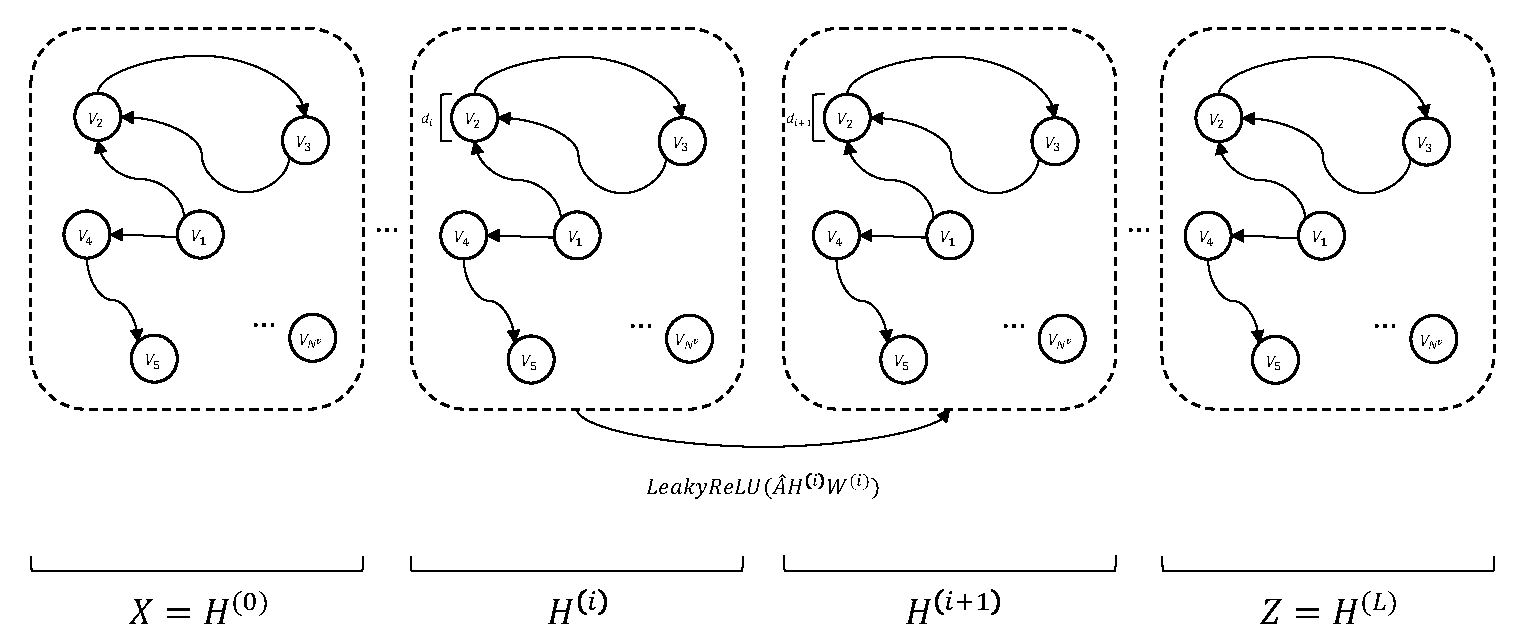
\includegraphics[width=1.0\linewidth]{ch2-gcn-modelov.pdf}
    \caption{The GCN training process}\label{fig:ch2-gcn-explain}
\end{figure}

\subsubsection{Design of Correlation Matrix}
%在GCN中,相关矩阵\(A\)表征了图节点之间的关系,GCN信息传播计算也是基于\(A\)进行的。因此,设计相关矩阵\(A\)是GCN模型的关键步骤。在该模型中,采用常用的数据关联规则挖掘算法Apriori算法,通过知识点共现次数统计来计算关联。 

%在该模型中,其实只需要找到知识点的对偶关系。因此,知识点关系矩阵可以表示为\(R/in \mathbb{R}^{T\time T}\)。第一个任务是找到标签集中频繁关联标签的出现次数。\(\operatorname{Support}\)、\(\operatorname{Confidence}\)和\(\operatorname{Lift}\)可以用来评估频繁标签集。支持度是指标签集中标签对的出现次数占总标签集的比例。置信度反映了一个标签\(L_i\)出现、另一个标签\(L_j\)出现的概率,或数据的条件概率。提升度表示标签\(L_i\)$同时包含的概率,以及X种群出现概率的比例。

In GCN, the correlation matrix \(A\) characterizes the relationship between graph nodes, and GCN information propagation calculation is also based on \(A\). Therefore, designing the correlation matrix \(A\) is a crucial step in the GCN model. In this model, the commonly used data association rule mining algorithm Apriori algorithm calculates knowledge point association by knowledge point reference co-occurrence statistics.

In this model, only the knowledge pairwise relationship needs to be found. Therefore, the knowledge point relationship matrix can be expressed as \(R\in \mathbb{R}^{T\times T}\). The first task is to find the number of occurrences of frequently associated label in the label set. The \(\operatorname{Support}\), \(\operatorname{Confidence}\), and \(\operatorname{Lift}\) can be used to evaluate frequent label sets. Support is the proportion of the number of occurrences of label pair in the label set in the total label set. Confidence degree reflects the probability of a label \(L_i\) appearing, another label \(L_j\) appears, or the conditional probability of the data. Lift represents the probability that the label \(L_i\) is contained at the same time, and the ratio of the probability of occurrence of X population:
\begin{align}
    \begin{split}
        \operatorname{Support}(L_i, L_j)       & =P(L_i,L_j)=\frac{\operatorname{number}(L_i,L_j)}{\operatorname{number}(\text{ All Samples })} \\
        \operatorname{Confidence}(L_i \to L_j) & =P(L_i \mid L_j)=P(L_i, L_j) / P(L_j)                                                \\
        \operatorname{Lift}(L_i \to L_j)       & =P(L_i \mid L_j) / P(L_i)=\operatorname{Confidence}(L_i \to L_j) / P(L_i)
    \end{split}
\end{align}

Similar to calculating Support, the frequency matrix \(E\in \mathbb{R}^{N^{(k)}\times N^{(k)}}\) of the sample knowledge point label pairs in the exercise training set can be calculated here. The \(M_{ij}\) represents the amount of co-occurrence between the knowledge point \(i\) and the knowledge point \(j\) in an exercise reference. Similarly, the knowledge point pair can be calculated by calculating Confidence to calculate the conditional probability matrix \(P\), where \(P_{ij}=P(L_i, L_j)/P(L_j)\), where \(P_{ij}=P(L_i, L_j)/P(L_j)\) means the situation when the knowledge point \(j\) appears The conditional probability of the occurrence of the following knowledge point \(i\).

It is a simple solution to directly set \(P\) as the incidence matrix \(A\), but in actual situations, some comprehensive questions in the exercise set contain practically unrelated knowledge points, but these situations are relatively rare. In order to exclude the interference of accidental circumstances, a minimum knowledge confidence threshold can be set. When \(P_{ij}\) is greater than the given threshold \(\tau^{(k)} \), naming activating value, then \(A_{ij}\) is set to \(P_{ij}\), Otherwise \(A_{ij}\) is set to 0. The formula is like \eqname{\ref{fml:confidence}}.

\begin{align}
    A_{ij}=\{\begin{array}{ll}
        0,      & \text{ if } P_{ij}<\tau^{(k)}      \\
        P_{ij}, & \text{ if } P_{ij} \geq \tau^{(k)}
    \end{array}\label{fml:confidence}
\end{align}


%该模型之所以采用GCN结构,是因为GCN对每个节点的参数共享,使得学习到的分类器可以在知识关联图中保留相关信息,从而隐性地表达其空间语义结构。因此,输出的分类器可以保留和识别隐含的知识标签依赖信息。对于知识点的依赖性,可以参考数据关联法挖掘算法,如apriori算法,通过计算习题中知识点的共现性来计算共相关矩阵。

This model adopts the GCN structure because the parameter sharing of GCN for each node allows the learned classifier to retain the associated information in the knowledge association graph, thereby implicitly expressing its spatial semantic structure. Therefore, the output classifier can retain and identify the implicit knowledge label dependent information. For the dependence of knowledge points, refer to the data association method mining algorithm such as Apriori algorithm~\cite{panjaitan2019implementation}, and calculate the co-relation matrix by calculating the co-occurrence of knowledge points in the exercises.


\subsubsection{Classifier generator}

%在所提出的基于GCN的模型中,知识点标签用词嵌入来表示。知识点集 \(K={k_1,k_2,\ldots,k_T} \),其中 \(T\)为知识点的总数。对于每一个单个知识点来说\(k_i\),\(k_i \in mathbb{R}^{Ttimes d^{(k)}}),\(d^{(k)})是知识点对象的嵌入向量的维度。本文采用可学习的堆栈式GCN网络将这些知识点对象逐一转化为内部连接的知识点对象分类器\(C=[c_1,c_2,\ldots,c_n]\),其中\(c_iin\mathbb {R}^{Ttimes d^{(r)}}\),\(d^{(r)}\)是文本挖掘模块输出的文本表示向量\(r\)的维度。这些分类器和\(r\)可以用来计算每个标签的点积。

In this thesis, a learnable stacked GCN-based model is proposed. The knowledge point labels are represented by knowledge label word embedding. Knowledge point set \(K=\{k_1,k_2,\ldots,k_{N^{(k)}}\} \), where \(N^{(k)}\) denotes the amount of knowledge points. For each single knowledge point \(k_i\), it is constrained that \(k_i \in \mathbb{R}^ {d^{(k)}}\), in which \(d^{(k)}\) is the dimensionality of the embedding vector of knowledge point object. The knowledge label word embedding set is the input of GCN, i.e., \(X = K\). The GCN is used to transform these knowledge point objects one by one into an internally connected knowledge point object classifier \(C=[c_1,c_2,\ldots,c_{N^{(k)}}\), where \(c_i \in \mathbb {R}^{d^{(r)}}\), \(d^{(r)}\) is the dimensionality of the text representation vector \(r\) output by the text mining module. These classifiers and \(r\) can be used to calculate the dot product of each label. The structure overview is proposed in \figname{\ref{fig:ch2-gcn-clsgen}}.

\begin{figure}[htbp!]
    \centering
    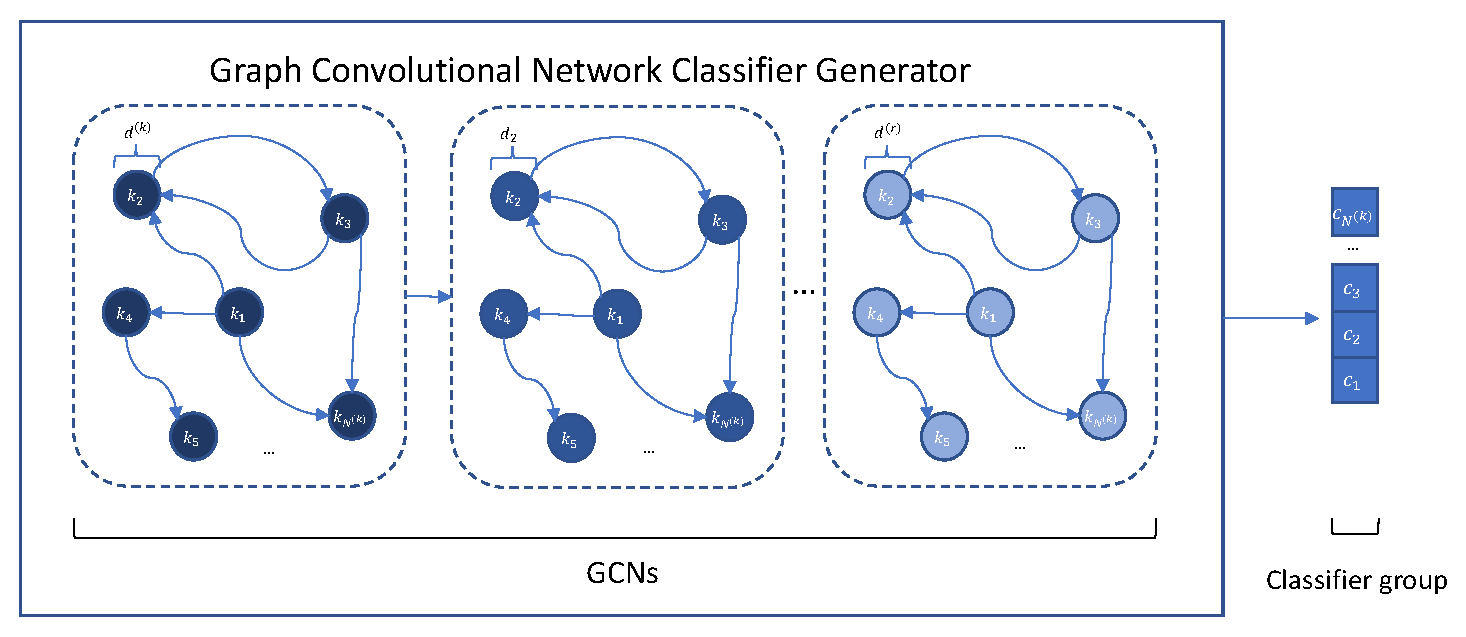
\includegraphics[width=1.0\linewidth]{ch2-gcn-clsgen.pdf}
    \caption{The structure of GCN-based classifier generator}\label{fig:ch2-gcn-clsgen}
\end{figure}

\subsection{Multi-label Recognition}
%  For the input layer, the input is \(r\in \mathbb{R}^{T \times d^{(k)}}\), where \(d^{(k)}\) is the number of dimensions represented by the embedding of the knowledge point object. Each GCN layer 1 takes the node representation from the previous layer \(H^{(l)}\) as input and outputs a new node representation \(H^{(l+1)}\). The output layer of the last layer is \(C\), where \(d_r\) represents the dimension of the title text. 

From the stacked GCN network, the object classifiers \(C=\{c_1,c_2,\ldots,c_{N^{(k)}}\} \) can be learned, where \(N^{(k)}\) represents the number of knowledge points. Finally, the label prediction vector \(\hat{y}\) can be obtained by the dot product of the learned classifier and the title text representation \(r\):
\begin{align}
    \hat{y} = C\times r
\end{align}

Through manual labeling, the real knowledge point labels of the exercises can be obtained: \(y\in \mathbb{R}^C\), \(y_i\in \{0,1\} \), \(y_i=0\) means that the exercise does not have knowledge points The label of \(i\), on the contrary, \(y_i=1\) means that the exercise has a label of knowledge point \(i\). The loss function \(\mathbf{L}\) can be written as:
\begin{align}
    \mathbf{L}=\sum_{i=1}^{T} y_i \log (\text{sigmoid}(\hat{y}_i))+(1-y_i) \log (1-\text{sigmoid}(\hat{y}_i))
\end{align}

\section{Experiments}
%本章提出了一个习题知识点多标签标注的模型,在本节中,先对数据集进行了介绍,接着介绍了一些Baseline性能的模型,然后结合多标签标注提出了对比的性能指标评估方案,最后给出对比结果和分析。
This chapter proposes a multi-label labeling model for exercise knowledge points. This section first introduces the data set, then introduces some baseline performance models, and then combines the multi-label labeling to propose a comparative performance indicator evaluation plan. Finally, Give comparison results and analysis.
\subsection{Dataset}
%本文中的实验数据来自于在线网站koolearn.com的带标签的高考数学考题以及模拟题(包含答案解析),通过爬虫爬取题干、答案解析等文本语料。其部分知识点关联模型可以表示为如下图结构。该数据集经过过滤和人工选择,共3374道试题,包含148个知识点,题均知识点为1.7个,其知识点分布如图所示。
The experimental data comes from the labeled college entrance examination math test questions and simulation questions (including answer analysis) on the online website. The text corpus, such as question stems and answer analysis, are crawled through crawlers. Part of the knowledge point association model can be expressed as the following structure.


The data set has been filtered and manually selected. There are 3374 test questions, including 148 knowledge points, with an average of 1.7 knowledge points. The distribution of several knowledge points is shown in the \figname{\ref{fig:ch2-model-knowledgenet}}.
\begin{figure}[htbp!]
    \centering
    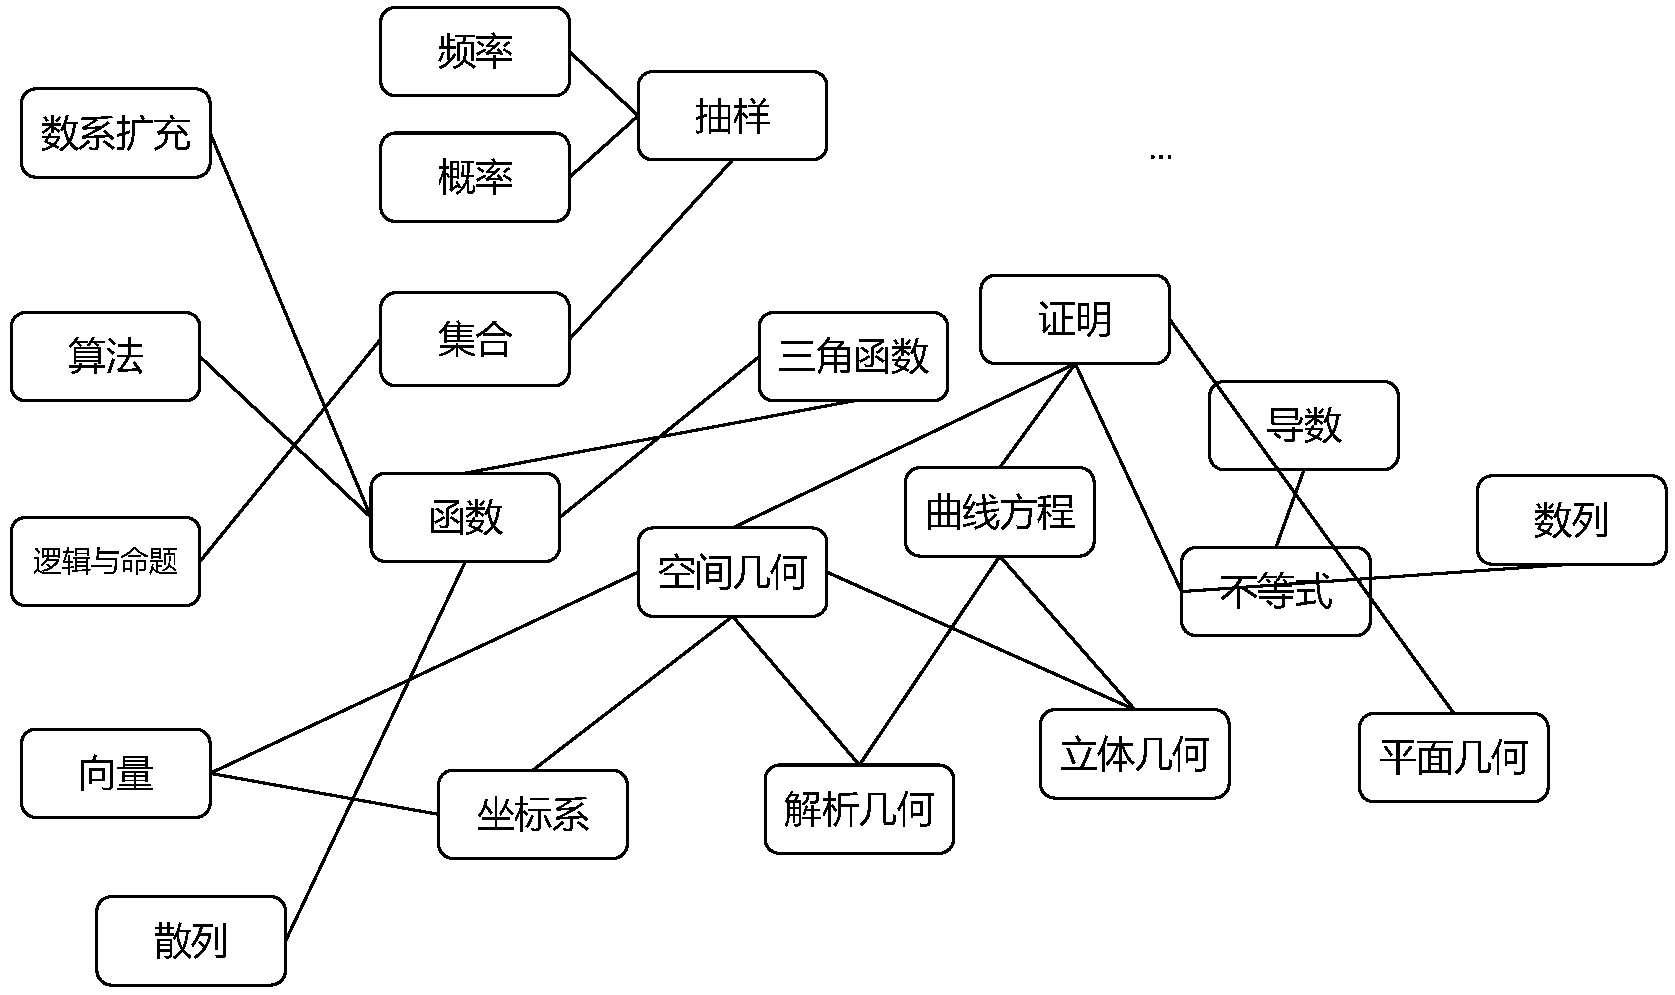
\includegraphics[width=1.0\textwidth]{ch2-model-knowledgenet.pdf}
    \caption{Knowledge points of dataset}\label{fig:ch2-model-knowledgenet}
\end{figure}

%该数据集的习题知识点数目分布如图所示。
The distribution of the number of exercise knowledge points in this data set is shown in the \figname{\ref{ch2-fig14}}.
\begin{figure}[htbp!]
    \centering
    \begin{subfigure}[b]{0.475\textwidth}
        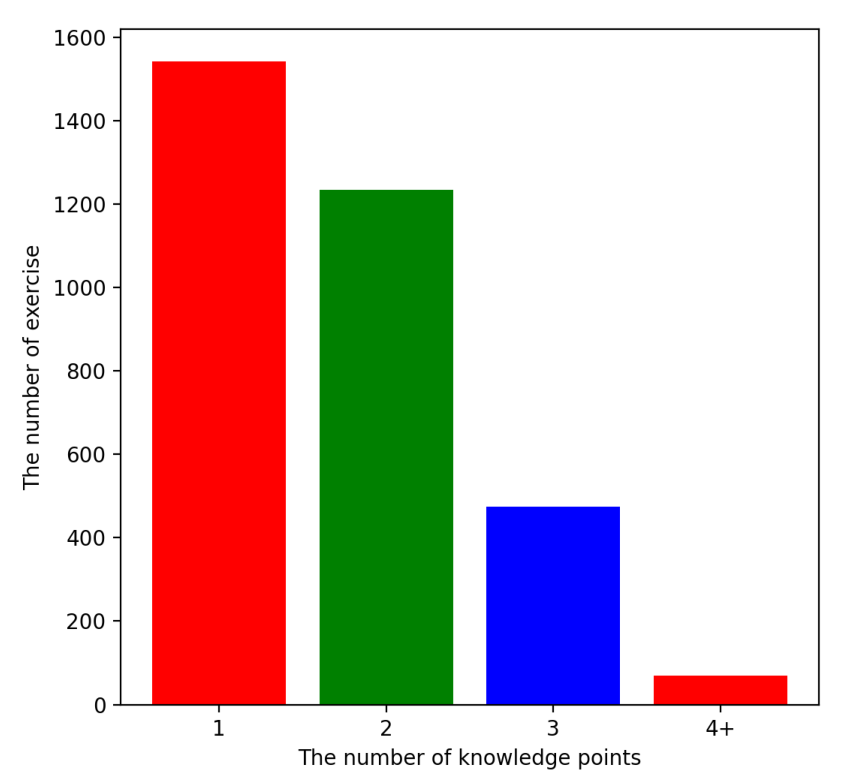
\includegraphics[width=0.9\textwidth]{ch2-fig14.pdf}
        \caption[dis]{Number of exercises}\label{fig:ch2-fig14-hist}
    \end{subfigure}
    \begin{subfigure}[b]{0.475\textwidth}
        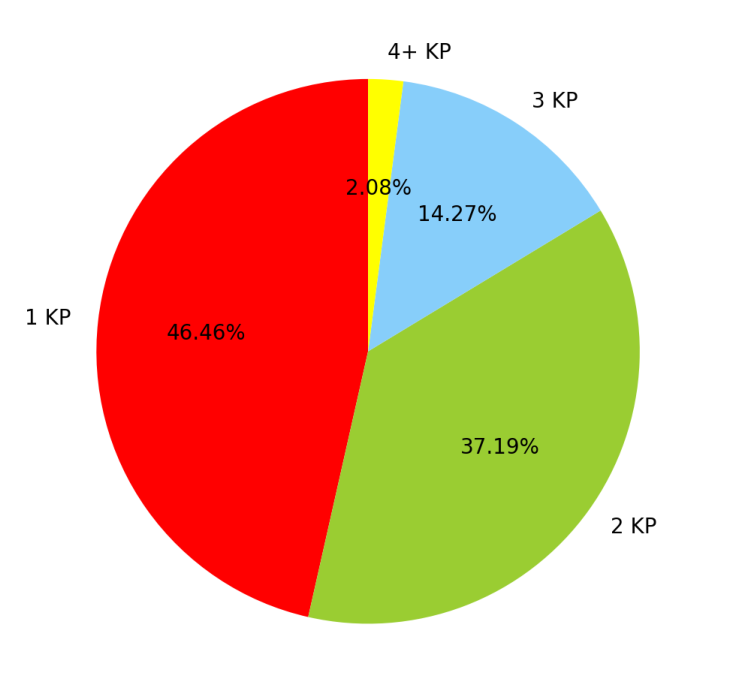
\includegraphics[width=0.9\textwidth]{ch2-fig15.pdf}
        \caption{Portion of exercises}\label{fig:ch2-fig14-pie}
    \end{subfigure}
    \caption{Distribution of the number of knowledge points of exercise}\label{ch2-fig14}
\end{figure}

% The experimental data in this thesis comes from high school math test questions in an online education platform database. The original data totals 2195, and 1357 test questions are obtained after the semi-automatic screening. The original labeled knowledge points are 166 items of original tags. After the mathematical knowledge point map is constructed and replaced, 61 tags are obtained.
\subsubsection{Data Prepartion}
%本节数据获取的方式为爬虫,因此获得的原始数据为大量非结构化的带有不规范数学符号的习题,这些符号难以被BERT模型处理,会带来误差,因此在预处理的过程中,会将无法识别的字符进行替换。另外还有大量的无意义文本,此外,由于部分习题知识点标注不全,因此需要人工协助标注知识点。
\subsection{Baseline}
% In the algorithm, the binary relation method (BR), the multi-label KN algorithm (ML-KNN) are selected as the comparison algorithm, and the experimental training set test set division ratio, which is 1:1.
% 目前,已经有一些进行文本标签标注的算法模型,为了验证本文提出算法的有效性,将与下列的算法进行比较,作为baseline指标。
At present, there are already some algorithm models for labeling text. To verify the effectiveness of the algorithm proposed in this thesis, the following baseline models will be set as comparisons.
\begin{itemize}
    \item Naive Bayes algorithm (NB): predict the labeling probability of a knowledge point based on the prior probability of text combination, and then convert the binary classification problem into a multi-label problem
    \item Multi-label KNN (ML-KNN): Proposed by Zhang et al.~\cite{zhang2007ml}, it searches the k instances closest to the instance through the KNN algorithm, counts the number of each category in the k samples, uses the Naive Bayes algorithm to generate prediction outcomes for each label.
    \item CNN+word2vec: Use word2vec to convert the test question text into an embedded vector, extract the test text information through CNN, and then output the multi-label prediction
    \item CNN+BERT\@: Use BERT to convert the test question text into an embedded vector, extract the test text information through CNN, and then output the multi-label prediction.
\end{itemize}

\subsection{Metrics}
%相比于传统学习问题,对多标签数据的标注十分困难,多标签意味着巨大的分类成本。本节的任务中,需要对试题进行多知识点标注,实际上是一个多标签分类问题,则样本维度、数据量、标签维度都会影响标注效果。本节利用了基于标签的评测方法来对提出的试题知识点标注模型进行性能评估。
Compared with traditional learning problems, it is tough to label multi-label data, and multi-label means huge classification cost~\cite{zhang2013review}. In the tasks in this section, the test questions need to be labeled with multiple knowledge points. It is a multi-label classification problem. The sample dimension, data volume, and label dimension will all affect the labeling effect. This section uses label-based metrics to evaluate the performance of the proposed test knowledge point labeling model.

%关于多标签分类,考虑到习题的标签之间的关系,本文使用了基于标签的指标来进行模型评估。该指标对每个标签分别进行混淆矩阵指标计算计算出True Positive,False Positive,True Negative和False Negative的样本值。然后计算F1指标值,以此进行多标签指标评估。

Regarding multi-label classification, considering the relationship between the exercises' labels, this thesis uses label-based indicators for model evaluation. The indicator calculates the confusion matrix indicator for each label to calculate the sample values of True Positive (TP), False Positive (FP), True Negative (TN), and False Negative (FN). Then calculate the macro-F1 and micro-F1 metrics for multi-label tagging model performance evaluation.

According to the metrics proposed by Zhou et al.~\cite{zhang2013review}, for the jth label of the ith example in the \(n\) examples, shown in the \eqname{\ref{fml:mlcm}}, where \(x_i\) and \(L_j\) represents the ith exercise and jth label, \(Y_i\) and \(\tilde{Y}_i\) represent the real labels and predicted labels of the ith exercise.

\begin{align}\label{fml:mlcm}
    \begin{split}
        \operatorname{TP}_j & =| \{x_i| L_j\in Y_{i}\wedge L_j \in \tilde{Y}_i , 1\leq i \leq n\}|       \\
        \operatorname{FP}_j & =| \{x_i| L_j\notin Y_{i}\wedge L_j \in \tilde{Y}_i , 1\leq i \leq n\}|    \\
        \operatorname{TN}_j & =| \{x_i| L_j\notin Y_{i}\wedge L_j \notin \tilde{Y}_i , 1\leq i \leq n\}| \\
        \operatorname{FN}_j & =| \{x_i| L_j\in Y_{i}\wedge L_j \notin \tilde{Y}_i , 1\leq i \leq n\}|
    \end{split}
\end{align}



%在混淆矩阵中,Precision为预测正确的正例数据占预测为正例数据的比例,Recall为预测为正例的数据占实际为正例数据的比例。F1值是精确率和召回率的调和均值,它是精确率和召回率的综合评价指标。其计算公式如下:

In the confusion matrix, Precision \(\operatorname{P}\) is the proportion of data with correct predictions to the data that is predicted to be positive, and Recall \(\operatorname{R}\) is the proportions of data with predictions that are positive to the actual data. The \(\operatorname{F1}\) value is the harmonic mean value of precision rate and recall rate, and it is a comprehensive evaluation index of precision rate and recall rate. The calculation formula is as \eqname{\ref{fml:f1score}}:

\begin{align}\label{fml:f1score}
    \begin{split}
        \operatorname{P}          & =\frac{\operatorname{TP}}{\operatorname{TP}+\operatorname{FP}}    \\
        \operatorname{R}          & =\frac{\operatorname{TP}}{\operatorname{TP}+\operatorname{FN}}    \\
        \operatorname{F1}_{score} & = \frac{2}{\frac{1}{\operatorname{P}}+\frac{1}{\operatorname{R}}}
    \end{split}
\end{align}


%micro F1 通过先计算总体的TP,FN和FP的数量,再计算F1, 而macro F1 分别计算每个类别的F1,然后做平均(各类别F1的权重相同)
Similarly, for the multi-label tagging problem, Macro F1 and Micro F1 can be used as the metrics. Micro-F1 first calculates the total number of TP, FN, and FP, and then calculates F1, while Macro-F1 calculates the F1 of each category separately and then averages (the weight of each category F1 is the same). The formula is \eqname{\ref{fml:f1-macro}} and \eqname{\ref{fml:f1-micro}}. The \(c\) is the total number of labels.

\begin{align}
    \operatorname{F1}_{macro} & =\frac{1}{c} \sum_{j=1}^{c} \operatorname{F1}_{score}(\operatorname{TP}_{j}, \operatorname{FP}_{j}, \operatorname{TN}_{j}, \operatorname{FN}_{j}) \label{fml:f1-macro}                                  \\
    \operatorname{F1}_{micro} & =\operatorname{F1}_{score}(\sum_{j=1}^{c} \operatorname{TP}_{j}, \sum_{j=1}^{c} \operatorname{FP}_{j}, \sum_{j=1}^{c} \operatorname{TN}_{j}, \sum_{j=1}^{c} \operatorname{FN}_{j}) \label{fml:f1-micro}
\end{align}

% 同样的,我们也可以基于样本统计一些指标。例如准确率,海明损失,查全率和F1值。准确率即预测标签完全正确的样本占总体样本的比例,海明损失为预测标签与真是标签的差距的度量指标,Precision和Recall分别代表真阳性样本占真样本的比例和真阳性样本占阳性样本的比例。它 们的计算公式为
Similarly, the statistic of some indicators based on samples can be obtained. For example, the multi-label accuracy rate \(\operatorname{Acc}_{ML}\), Hamming loss \(\operatorname{HmLoss}\), multi-label precision rate \(\operatorname{Precision_{ML}}\), multi-label recall rate \(\operatorname{Recall_{ML}}\) and \(\operatorname{F1}_{ML}\) can be calculated. Accuracy is the proportion of samples with completely correct predicted labels in the overall sample. Hamming loss is a measure of the difference between the predicted label and the true label. Precision and Recall represent the proportion of true positive samples in true samples and the proportion of true positive samples in positive samples proportion. Their calculation formulas are \eqname{\ref{fml:subaccuracy}}-{\ref{fml:f1scoreh}}.
\begin{align}
    \operatorname{Acc}_{ML}       & =\frac{1}{n} |\{i|Y_i=\tilde{Y}_i\}| \label{fml:subaccuracy}                                                                              \\
    \operatorname{HmLoss}         & =\frac{1}{n} \sum_{i=1}^{n} \frac{\operatorname{XOR}(Y_i,\tilde{Y}_i)}{c} \label{fml:hmloss}                                              \\
    \operatorname{Precision_{ML}} & =\frac{1}{n} \sum_{i=1}^{n} \frac{|Y_{i} \cap \tilde{Y}_i|}{|\tilde{Y}_i|} \label{fml:Precisionh}                                         \\
    \operatorname{Recall_{ML}}    & =\frac{1}{n} \sum_{i=1}^{n} \frac{|Y_{i} \cap \tilde{Y}_i|}{|Y_{i}|}    \label{fml:Recallh}                                               \\
    \operatorname{F1}_{ML}        & =\frac{2 \cdot \operatorname{Precision} \cdot \operatorname{Recall}}{\operatorname{Precision}+\operatorname{Recall}} \label{fml:f1scoreh}
\end{align}

\subsection{Setting and Environment}
The distribution of the number of exercise knowledge points in this data set is shown in the figure. The number of questions involved in different knowledge points is different. The set of questions involved in knowledge points \(j\) is defined as \(\mathbf{E}_j\). Remember the threshold of the number of occurrences of the knowledge point label \(\tau^{(KP)} \), then the knowledge points of the exercises can be divided according to the frequency of occurrence, i.e., \( \{j|\mathbf{E}_j|>\tau^{(KP)}\} \) and \( \{j||\mathbf{E}_j|\leq\tau^{(KP)} \} \). According to the different thresholds, the model's ability to classify knowledge points frequently and appear sparse can be tested separately.

%在实验中,设定了200,150,100,50,10五组阈值\(\tau^{(KP)} \),将具有标签\(j\)的习题记作\(\mathbb{E}_j\),则可以统计符合要求的标签集\(\mathbb{L}={j||\mathbb{E}_j|\geq\tau^{(KP)}}\)出习题集大小\(|\mathbb{E}_j|\)和题均知识点数\(LAvg_j \)。
In the experiment, five sets of thresholds of 200, 150, 100, 50, 10 are set \(\tau^{(KP)} \), and the exercises with the label \(j\) are recorded as \(\mathbf{E}_j\), the label set that meets the requirements can be counted as \(\mathbf{L}_\tau^{(KP)}=\{j\mid |\mathbf{E}_j|\geq\tau^{(KP)}\} \), the exercises containing label in \(\mathbf{L}_\tau^{(KP)} \) is denoted as \(\mathbf{E}_\tau^{(KP)} \), within which the average number of knowledge points of the exercise in the set is \(\overline{L}\).

\begin{table}[htbp!]
    \centering
    \caption{Setting of experiment}\label{tbl:ch2-ex1}
    \begin{tabular}{cccc}%{cp{2cm}<{\centering}p{2cm}<{\centering}p{2cm}<{\centering}}
        \toprule
        \text{\(\tau^{(KP)} \)} & \(|\mathbf{L}_{\tau^{(KP)}}|\) & \(|\mathbf{E}_{\tau^{(KP)}}| \) & \(\overline{L}\) \\
        \midrule
        200                     & 2                              & 463                             & 1.21             \\
        100                     & 22                             & 1376                            & 1.55             \\
        50                      & 29                             & 2237                            & 1.42             \\
        10                      & 57                             & 3158                            & 1.35             \\
        \bottomrule
    \end{tabular}
\end{table}

The running environment are shown in \tblname{{\ref{tbl:ch2-exp-env}}}.

\begin{table}[htbp!]
    \caption{Experiment running environment}\label{tbl:ch2-exp-env}
    \centering
    \begin{tabular}{l c}
        \toprule
        Software/Hardware & Configuration   \\
        \midrule
        CPU               & i7 9700K        \\

        GPU               & Tesla V100      \\

        Operating System  & Ubuntu 20.04    \\

        Python            & 3.8.6           \\

        PyTorch           & 1.6.0           \\

        GPU Driver        & Cuda10.1/cudnn7 \\
        \bottomrule
    \end{tabular}
\end{table}


There are many adjustable parameters of the model in BERT and GCN\@. Hyperparameters are shown in \tblname{\ref{tbl:ch2-hpsetting}}.
\begin{table}[htbp!]
    \caption{Hyperparameter settings of recommendation model}\label{tbl:ch2-hpsetting}
    \centering
    \begin{tabular}{l c c}
        \toprule
        Hyperparameter            & Value \\
        \midrule
        Transformer Layers        & 12    \\
        Dimension of hidden layer & 768   \\
        Optimizer                 & Adam  \\
        Learning Rate             & 0.001 \\
        LSTM dimension            & 150   \\
        batch size                & 32    \\
        Dropout                   & 0.3   \\
        \midrule
        \bottomrule
    \end{tabular}
\end{table}



%本实验中,定义了一个GCN架构用于学习知识点间关联,该架构包含两层GCN层,其维度分别为512和1024。每个节点采用256维word2vec来训练标签文本得到标签embedding表示。对于标签correlation阈值\tau则分别设置为多个值来进行模型性能判定。

% In this experiment, a GCN architecture is defined to learn the association between knowledge points. The architecture contains two GCN layers with dimensions of 512 and 1024, respectively. Each node uses 256-dimensional word2vec to train the label text to obtain the label embedding representation. The tag correlation threshold \(\tau \) is set to multiple values to determine the model performance.

% The running environment is Ubuntu 20.04, TensorFlow 2.23, Python 3.8.6, and the hardware is equipped with a Tesla V100 computing card. For each Baseline model, five rounds of calculation are performed, the maximum positive deviation and the minimum negative deviation are discarded, and the average value is recorded.

\subsection{Result and Analysis}
%,对于提出的模型,将标签得到如下的对比实验结果。
%对比实验结果分为横向baseline模型性能对比(得到表1和表2.)和模型不同超参数性能对比(表3)。
% \begin{table}
% 	\caption{Even better looking table using booktabs}\label{tbl:good_table}
% 	\centering

% 	\begin{tabular}{l c c c c}
% 		\toprule
% 		\multirow{2}{*}{Dental measurement} & \multicolumn{2}{c}{Species I} & \multicolumn{2}{c}{Species II}                \\
% 		\cmidrule{2-5}d
% 		                                    & mean                          & SD                             & mean  & SD   \\
% 		\midrule
% 		I1MD                                & 6.23                          & 0.91                           & 5.2   & 0.7  \\

% 		I1LL                                & 7.48                          & 0.56                           & 8.7   & 0.71 \\

% 		I2MD                                & 3.99                          & 0.63                           & 4.22  & 0.54 \\

% 		I2LL                                & 6.81                          & 0.02                           & 6.66  & 0.01 \\

% 		CMD                                 & 13.47                         & 0.09                           & 10.55 & 0.05 \\

% 		CBL                                 & 11.88                         & 0.05                           & 13.11 & 0.04 \\
% 		\bottomrule
% 	\end{tabular}
% \end{table}

The comparison experiment results are divided into the performance comparison of the horizontal baseline model (obtained in \tblname{\ref{tbl:bsline1}}-\ref{tbl:bsline4}).

\begin{table}[htbp!]
    \caption{Result comparison (\(\tau^{(KP)}=200 \))}\label{tbl:bsline1}
    \centering
    \begin{tabular}{cccccccc}
        \toprule
        Metrics      & \(\operatorname{F1}_{macro}\) & \(\operatorname{F1}_{micro}\) & \(\operatorname{Acc}_{ML}\) & \(\operatorname{HmLoss}\) & \(\operatorname{F1}_{ML}\) \\
        \midrule
        NB           & 75.3                          & 74.2                          & 69.6                        & 18.2                      & 73.6                       \\
        ML-KNN       & 77.1                          & 76.2                          & 73.2                        & 17.4                      & 76.3                       \\
        CNN+word2vec & 79.5                          & 78.4                          & 76.6                        & 14.2                      & 79.6                       \\
        CNN+BERT     & 80.1                          & \textbf{79.9}                 & 76.9                        & 13.7                      & 79.5                       \\
        Proposed     & \textbf{80.9}                 & 79.1                          & \textbf{77.3}               & \textbf{13.1}             & \textbf{80.7}              \\
        \bottomrule
    \end{tabular}
\end{table}

\begin{table}
    \centering
    \caption{Result comparison (\(\tau^{(KP)}=100 \))}\label{tbl:bsline2}
    \begin{tabular}{cccccccc}
        \toprule
        Metrics      & \(\operatorname{F1}_{macro}\) & \(\operatorname{F1}_{micro}\) & \(\operatorname{Acc}_{ML}\) & \(\operatorname{HmLoss}\) & \(\operatorname{F1}_{ML}\) \\
        \midrule
        NB           & 71.2                          & 72.1                          & 67.2                        & 16.2                      & 71.8                       \\
        ML-KNN       & 73.2                          & 72.3                          & 69.1                        & 15.9                      & 74.7                       \\
        CNN+word2vec & 74.3                          & 74.4                          & 72.3                        & 13.2                      & 75.2                       \\
        CNN+BERT     & 74.4                          & 74.6                          & 72.3                        & 13.1                      & 75.1                       \\
        Proposed     & \textbf{75.5}                 & \textbf{75.7}                 & \textbf{73.1}               & \textbf{12.7}             & \textbf{74.9}              \\
        \bottomrule
    \end{tabular}
\end{table}

\begin{table}
    \centering
    \caption{Result comparison (\(\tau^{(KP)}=50 \))}\label{tbl:bsline3}
    \begin{tabular}{cccccccc}
        \toprule
        Metrics      & \(\operatorname{F1}_{macro}\) & \(\operatorname{F1}_{micro}\) & \(\operatorname{Acc}_{ML}\) & \(\operatorname{HmLoss}\) & \(\operatorname{F1}_{ML}\) \\
        \midrule
        NB           & 52.3                          & 53.0                          & 42.1                        & 9.2                       & 51.9                       \\
        ML-KNN       & 44.2                          & 43.9                          & 23.5                        & 10.1                      & 42.1                       \\
        CNN+word2vec & 56.1                          & \textbf{57.3}                 & 46.2                        & 8.2                       & 56.5                       \\
        CNN+BERT     & 56.2                          & 56.8                          & \textbf{47.0}               & \textbf{8.1}              & 56.1                       \\
        Proposed     & \textbf{57.1}                 & 57.2                          & 45.2                        & 8.6                       & \textbf{57.5}              \\
        \bottomrule
    \end{tabular}
\end{table}

\begin{table}
    \centering
    \caption{Result comparison (\(\tau^{(KP)}=10 \))}\label{tbl:bsline4}
    \begin{tabular}{cccccccc}
        \toprule
        Metrics      & \(\operatorname{F1}_{macro}\) & \(\operatorname{F1}_{micro}\) & \(\operatorname{Acc}_{ML}\) & \(\operatorname{HmLoss}\) & \(\operatorname{F1}_{ML}\) \\
        \midrule
        NB           & 36.5                          & 37.1                          & 26.1                        & 4.2                       & 36.5                       \\
        ML-KNN       & 30.1                          & 32.1                          & 29.1                        & 3.6                       & 32.5                       \\
        CNN+word2vec & 36.7                          & 38.2                          & 37.5                        & 3.5                       & 37.2                       \\
        CNN+BERT     & 36.9                          & \textbf{38.6}                 & \textbf{38.6}               & \textbf{3.5}              & 37.5                       \\
        Proposed     & \textbf{37.1}                 & 38.3                          & 35.4                        & 3.8                       & \textbf{38.6}              \\
        \bottomrule
    \end{tabular}
\end{table}

%从表中可以看出,本文提出的模型在出现频次较高的习题训练机上的性能表现强于Baseline模型。随着知识点出现频率的降低,分类的难度增大,所有模型都出现了性能退化现象。其中的原因是模型对于出现较少的标签无法进行有效的信息抓取,从而产生的误差增大。总体而言,在F1-Score参数和较为严格的子集准确率指标上,本文提出的模型都取得了最优或较优的性能表现。当习题标签频次出现次数非常低时,几乎所有的模型都无法取得较好的结果,这是因为由于习题标签的频次分布不均匀,少量冷门标签无法很好地标注,导致模型训练出现了过拟合现象从而影响标注表现。为了解决该问题,可以通过用更大和知识点出现频次较为平均的习题集作为训练集来优化模型预测性能表现。

It can be seen from the table that the performance of the model proposed in this thesis is stronger than the baseline model on the exercise training machine with a higher frequency. As the frequency of knowledge points decreases, classification difficulty increases and performance degradation occurs in all models. The reason is that the model cannot effectively capture information for fewer tags, resulting in increased errors. In general, the model proposed in this thesis has achieved the best or better performance in terms of F1-Score parameters and stricter subset accuracy indicators. When the problem labels' frequency is shallow, almost all models cannot achieve good results. This is because due to the uneven frequency distribution of the problem labels, a small number of unpopular labels cannot be well labeled, resulting in over-fitting in model training. This phenomenon affects labeling performance. In order to solve this problem, the model prediction performance can be optimized by using a larger set of exercises with a more average frequency of knowledge points than the training set.

% From the experimental results, it can be seen that, compared with the binary relation method, the multi-label KNN algorithm, and the classifier chain method, the multi-knowledge point labeling method based on ensemble learning proposed in this thesis has achieved better results under different knowledge point labels. In multi-label classification, the evaluation of more stringent indicators—subset accuracy-this thesis's method is always significantly better than the other three methods. Screening the base classifiers with relatively good performance and integrating their results through the majority voting method compensated for each base classifier's disadvantages and obtained good results. However, as the tag frequency threshold decreases, the number of knowledge points gradually increases, and the difficulty of multi-label classification becomes more and more difficult. One of the reasons is that the knowledge points actually contained in a test question is not completely consistent with the knowledge points that the teacher investigates. As shown in Table 7, in the first three questions, there is no ``arithmetic sequence'' in the original manually labeled knowledge points, but the content of the test questions contains the term ``arithmetic sequence''. Questions 4 and 5 The knowledge point is ``arithmetic sequence'', and there is also ``arithmetic sequence'' in the question stem. Therefore, when using the trained model to predict the first three questions, the ``arithmetic sequence'' will be marked as the knowledge point of this question. It is more difficult to further determine the knowledge points of examination questions and the knowledge points contained in the questions based on the existing data. The second reason is that due to the uneven distribution of knowledge points, many knowledge points do not have enough test data for learning, which makes it difficult to predict the knowledge points in the pre-test questions.


\section{Summary}
%在习题推荐系统中,有数量众多的知识点标签缺失的习题,为了满足自适应学习系统的要求,需要对习题进行知识点标注,但人工标注成本较高,效率较低。因此, 自动标注试题知识点成为了亟待解决的问题。本章提出了一个基于图卷积神经网络和基于注意力机制的Bi-LSTM文本挖掘模型的习题多知识点标注模型。经过对实验数据集的验证,取得了相对现有模型的较好的知识点标注效果。

%本章的贡献有以下几点:
%(1)通过图神经网络表征知识点间的关系,从而可以挖掘出原文本中隐藏的知识点标签,给现有的模型提供了知识点标签联想推理功能。
%(2)通过设计知识点间关联函数,对知识点间依赖进行建模,并取得了较好的性能表现。
%(3)验证了低知识点标签频次对于多标签分类模型会产生过拟合现象,从而造成性能退化,为了解决该问题,可以通过平均训练数据集标签频次来解决。

%习题知识点标注是推荐系统的第一步,经过标注的习题可以作为知识追踪模型的输入,从而追踪学生的知识状态,也可以作为推荐系统的输入特征来完成基于知识点的习题推荐。

In the exercise recommendation system, there are a large number of exercises with missing knowledge point labels. It is necessary to label the exercises to meet the adaptive learning system's requirements, while the manual labeling cost is high and the efficiency is low. Therefore, automatic marking of knowledge points of test questions has become an urgent problem to be solved. This chapter proposes a multi-knowledge point labeling model for exercises based on GCN and Bi-LSTM text mining model based on the attention mechanism. A better knowledge point labeling effect than existing models has been achieved after verifying the experimental data set.

The contributions of this chapter are as follows:
\begin{enumerate}
    \item The relationship between knowledge points is represented by a graph neural network, which can dig out the hidden knowledge point labels in the original text and provide the existing model with the knowledge point label association reasoning function.
    \item By designing the correlation function between the knowledge points, the dependence between the knowledge points is modeled, and good performance has been achieved.
    \item It is verified that the low-knowledge point label frequency will produce an over-fitting phenomenon for the multi-label classification model, resulting in performance degradation. It can be solved by averaging the label frequency of the training data set.
\end{enumerate}

The labeling of exercise knowledge points is the first step of the recommendation system. The labeled exercises can be used as the input of the knowledge tracking model to track students' knowledge state and can also be used as the recommendation system's input feature to complete the recommendation of exercises based on knowledge points.


\chapter{Graph Attention Networks Embedded Knowledge Tracing Model With Transformer}

% **************************** Define Graphics Path **************************
\ifpdf
    \graphicspath{{Chapter3/Figs/Raster/}{Chapter3/Figs/PDF/}{Chapter3/Figs/}}
\else
    \graphicspath{{Chapter3/Figs/Raster/}{Chapter3/Figs/Vector/}{Chapter3/Figs/PDF/}{Chapter3/Figs/}}
\fi

\section{Research Motivation}
%本章节为该推荐系统的一个核心部分,即通过知识追踪的方式获取学生的知识掌握状态。该模型用于评估学生的知识掌握状态,在后续的推荐模型中作为推荐的基础依据。知识追踪是一种常见的用于学生的认知诊断的模型,它根据学生的以往的答题记录来建模学生的知识掌握情况,从而获取学生的知识状态。知识追踪的模型非常丰富,早期的知识追踪模型贝叶斯知识追踪(BKT),它们的基础假设是学生答题基于一系列知识点,这些知识点之间被认为是相互不相关的,因此它们之间是独立表示,这种做法无法捕捉不同概念之间的关系也无法表征复杂的概念转换。在2015年,Piech等人提出了深度知识追踪模型(DKT),首次将长短期记忆网络(LSTM)应用于知识追踪任务,它无需进行知识点标注,而是包含一个知识的隐含状态,当时取得了超过BKT的基线性能,它标志着基于神经网络模型的知识追踪研究的序幕。但DKT无法输出知识的隐藏状态,可解释性不足。而且DKT用将所有记忆存储于一个隐藏向量中,对于长序列的预测性能不够理想。针对这个问题,记忆增强网络(MANN)被提出来,它允许网络保留多个隐藏状态向量,并分别读写这些向量。在2017年,张等人提出了Dynamic Key-Value Memory Networks(DKVMN),它参考了MANN的设计,针对知识追踪任务进行了优化,优化了MANN对于知识追踪任务的输入输出不同域的问题。DKVMN采用了键值对作为存储器结构,能避免过拟合、参数少,以及通过潜在概念自动发现相似练习,取得了相对BKT和DKT更好的预测性能。同时该模型也具有较好的可解释性,它将问题相关潜在概念存储于键矩阵中,对概念掌握程度存储于值矩阵中,通过对输入练习与键矩阵的相关性对值矩阵进行更新。

%尽管该模型取得了较好的性能,但该模型将知识点建模为相互独立的点,而未考虑知识点之间的关联性。在高中数学知识网络中,知识点与知识点间有网状的关联关系,而习题是基于这些知识点建立的。因此习题与习题之间也存在隐含的间接关联关系,因此设计一种将考虑知识点间关联的模型来表征该模型是一种合理的解决方案。除了考虑习题知识点的掌握程度,对于学生的答题行为也可以作为额外的特征加入该模型,这样可以为模型增加更多的考虑因素,从而增强模型的预测性能。本文提出了一种用图神经网络结合记忆增强网络的知识追踪模型。该模型相对于原始的DKVMN模型,用图神经网络改造了知识点表征矩阵,并将学生的额外答题行为特征作为模型输入。

This section is a core part of this recommendation system to obtain the student's knowledge mastery status using knowledge tracing. The model is used to assess the student's knowledge acquisition status, which is used as the basis for recommendations in the subsequent recommendation model. Knowledge tracing is a common model used for the cognitive diagnosis of students, which models students' knowledge acquisition based on their previous answer records to obtain their knowledge status~\cite{gonzalez2014general}. There is a wealth of models for knowledge tracing, early models of knowledge tracing Bayesian Knowledge Tracing (BKT)~\cite{yudelson2013individualized}, which issued the assumption that students' solutions to exercises are based on a set of knowledge points that are considered to be unrelated to each other and are therefore represented independently of each other. This approach fails to capture the relationships between different concepts nor to characterize complex conceptual transformations. In 2015, Piech et al. proposed the deep knowledge tracing model (DKT), which first applied RNN to the knowledge tracing task, which contains an implicit state of knowledge, and achieved a baseline performance over BKT at that time, and it marked the prologue of knowledge tracing research based on neural network models. However, DKT cannot output the hidden state of knowledge and is not sufficiently interpretable.

Moreover, DKT uses to store all memories in a hidden vector, and the prediction performance for long sequences is not satisfactory enough. Memory Augmented Neural Network (MANN)~\cite{santoro2016meta} was proposed to address this problem, which allows the network to keep multiple hidden state vectors and read and write these vectors separately. In 2017, Dynamic Key-Value Memory Networks (DKVMN)~\cite{zhang2017dynamic} referring to the design of MANN for knowledge tracing tasks and optimizes MANN for knowledge tracing tasks with different input and output domains. DKVMN uses key-value pairs as the memory structure, which can avoid over better prediction performance relative to BKT, and DKT is achieved by using key-value pairs as the memory structure, which can avoid overfitting. The model also has better interpretability. It stores the problem-related potential concepts in the key matrix and the mastery proficiency to the concepts in the value matrix and updates the value matrix by correlating the input exercises with the key matrix.

Although the model achieved better performance, the model modeled knowledge points as mutually independent points without considering the correlations. There are web-like correlations between knowledge points in the high school mathematics knowledge network, and the exercises are built based on these knowledge points. Therefore, there are also implicit and indirect correlations between the exercises and the exercises, so it is reasonable to design a model that will consider the correlations between knowledge points to characterize the model. In addition to considering the degree of mastery of the exercises' knowledge points, the students' answering behaviors can also be added to the model as additional features, adding more consideration to the model and enhancing the model's predictive performance. This thesis proposes a knowledge tracing model using graph neural networks combined with memory enhancement networks. The model transforms the knowledge point representation matrix with graph neural networks relative to the original DKVMN model and uses additional characteristics of students' answering behaviors as model inputs.

\section{Research Contribution}
%DKVMN模型有如下的问题,第一,该模型未考虑学生的特性,每个学生对于潜在知识点的掌握程度会导致不同的结果,即,当两个知识点掌握程度相同的学生可能对于一个习题的作答结果会产生不同的预测度。第二,该模型未考虑知识点的内在联系,该模型将知识点作为存储结构中的一个slot,各个slot之间相互独立。这隔绝了知识点变化引起的相关知识点的变化。在高中数学学科中,有许多相互相关的知识点,因此,需要结合领域特征,加入知识点关联学习网络。本文基于上述两点,对DKVMN模型进行改进。
In this section, an improved knowledge tracing model is proposed based on the DKVMN structure. The DKVMN model is improved based on the above two points. The DKVMN model has the following problems. First, the model does not take into account the characteristics of students, and each student's mastery of potential knowledge points will lead to different results, i.e., when two students with the same level of mastery of knowledge points may have different prediction degrees for the answer results of an exercise. Second, the model does not consider the intrinsic connection of the knowledge points, which are treated as a slot in the storage structure, and each slot is independent of others. This prevents the changes in related knowledge points caused by changes in knowledge points. In high school mathematics subjects, there are many interrelated knowledge points. Therefore, it is necessary to incorporate the domain characteristics and join the knowledge point associated learning network.

\section{Related Theory}
\subsection{Knowledge Tracing}
%知识追踪为智能化和自适应教育提供了条件,它具有个性化和自动化的特点。知识追踪任务从学生的历史学习记录来追踪学生的知识状态变化,预测未来的学习表现,从而针对性地给予学习辅导。其本质基于学生的过去的学习表现来获取当前的学习状态,从而预测将来的学习表现。其实际做法是,对学生过去的答题记录进行数据分析和过程建模,从而建模当前的学生学习状态数据,让模型跟做学生的每个阶段的学习状态,并基于学习状态数据来预测习题答对的概率。在学科学习中,学科知识由一系列知识点组成,学生的学习状态实际上基于对于各个知识点的掌握情况。而知识追踪一般的形式为给定一个学生的答题序列,该序列由一系列习题构成,习题又与特定的知识点相关联,在知识追踪中的一个基本假设是,学生的答题表现基于对知识点的掌握。而学生的答题表现即可用于反推学生对于各个知识点的掌握情况,即学习状态的掌握情况。

%知识追踪任务的数学表示为一个学生在一个习题序列上的交互式答题记录\(X_t=(x_1,x_2,\ldots,x_t)\),根据该记录通过建模来获取学生的学习状态,并预测学生在下一次练习中的表现$x_{t+1}$。其中$x_t$通常表示为一个有序对$(q_t,a_t)$,有序对表示学生在时间$t$回答了问题$q_t$,$a_t$表示问题的得分情况,也有许多知识追踪任务用答对或答错来表示,此时$a_t$为0或者1,在此情况下,实际上预测的是对于下一个问题回答正确的概率$P(a_{t+1}=1|a_t)$。如图ref{kt1}。

Knowledge tracing provides the conditions for intelligent and adaptive education, which is personalized and automated. Knowledge tracing tracks students' knowledge status from their historical learning records, predicts future learning performance and provides targeted learning coaching. The essence is to obtain the current learning status based on the student's past learning performance to predict the future learning performance. The actual practice is to analyze the data and process modeling of students' past answer records to model the current student learning status data and let the model follow the learning status of students at each stage, and predict the probability of correct answers to the exercises based on the learning status data. In subject learning, subject knowledge consists of a series of knowledge points, and students' learning status is based on their mastery proficiency to each elementary knowledge concept. The general form of knowledge tracing is that given a sequence of student answers, which consists of a series of exercises associated with a specific knowledge point, a fundamental assumption in knowledge tracing is that student performance is based on mastery proficiency to the knowledge concept. The student's performance can be applied to infer the student's mastery proficiency for each knowledge concept, i.e., the mastery proficiency to the learning state.

The mathematical representation of the knowledge tracing task is an interactive answer record \(X_t=(x_1,x_2,\ldots,x_{t-1})\) of a student on an exercise sequence, based on which the student's learning status is obtained by modeling and predicting the student's performance in the next exercise \(x_{t}\). Where \(x_t\) is usually represented as an ordered pair \((q_t,a_t)\), the ordered pair indicates that the student answered the exercise \(q_t\) at time \(t\), and \(a_t\) indicates the score of the exercise, also many knowledge tracing tasks are represented by correct or incorrect answers, when \(a_t\) is 0 or 1. In this case, what is actually predicted is the probability of answering correctly for the next exercise \(P(a_{t}=1|a_{t-1},\ldots,a_1)\). As shown in the figure \figname{\ref{fig:ch3-model-ktdes}}.

\begin{figure}[htbp!]
    \centering
    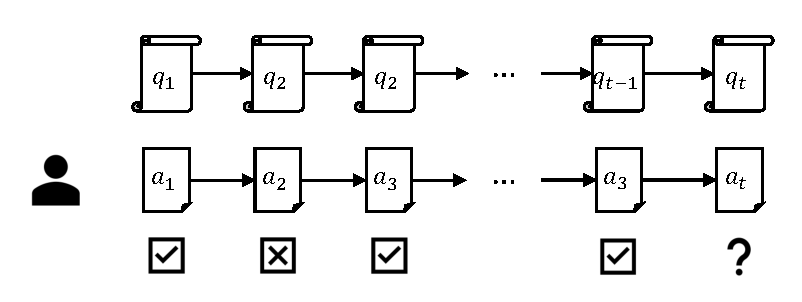
\includegraphics[width=0.9\textwidth]{ch3-kt-model.pdf}
    \caption{The knowledge tracing pattern}\label{fig:ch3-model-ktdes}
\end{figure}

\subsection{Dynamic Key-Value Memory Networks}
%在传统的机器学习模型中,逻辑流控制和外部记忆机制往往缺失。因此,许多当前的机器学习模型无法建立复杂的逻辑流控制和外部记忆模块。传统的模型往往无法高效地利用可训练参数来获得较强记忆能力的模型。目前像LSTM和GRU这些结构,具备一定的记忆能力,但该能力受可训练参数数目影响,记忆增强网络通过更强的表征能力来摆脱可训练参数数目与模型的记忆能力之间的联系。它能够模拟人脑的工作记忆机制,例如阅读理解、推理、运算过程等,也可以捕捉复杂的结构信息和建立长距离信息依赖。MANN将中间信息保留在内存中,形成一个信息缓存结构,并利用该信息进行后续的推理学习。在一个MANN网络中往往分为控制器、存储模块和读写器等三个部分。控制器读取前一阶段的状态和当前的输入来获取下一阶段的输出和控制器输出。存储模块是一个数据结构模型,例如栈、队列或数组,每一个时刻都通过一个输出函数处理读取内容和控制器输出来计算序列输出。

%在知识追踪任务中,由于习题所包含的知识点表征与知识点掌握状态表征所处的空间不同,因此无法将掌握程度和知识点表征用一个存储结构来保存,因此需要对MANN模型进行改造来适配知识追踪任务。DKVMN通过将知识点表征保存在一个矩阵\(M^{(k)}\)中作为Keys,将对应知识点掌握表征保存在另一个矩阵\(M^{(v)}\)中,作为Values。在输入一个习题表示\(q_t\)时,模型将\(q_t\)的嵌入表示向量\(k_t\)与知识点表征模块\(M^{(k)}\)进行相关度计算,得到习题的知识点相关度表示向量\(w_t\)。每个习题都可以表示为一个与知识点的相关度向量,代表了与知识点的相互关系。在DKVMN模型中,有读取过程和写入过程。

%在读取过程中,模型将权重向量\(w_t\)与知识点掌握矩阵\(M^{(v)}\)进行加权和计算,获得用户对于知识点的掌握表征向量\(r_t\)。并将\(r_t\)与当前的习题嵌入向量\(k_t\)进行拼接,经过全联接激活层输\(Tanh(\cdot)\)出\(f_t\),它表示用户对于习题的掌握程度。\(f_t\)会经过一个最终的\(Sigmoid(\cdot)\)激活函数来输出一个习题回答正确的预测概率\(p_t\)。在写入过程中,当前的实际回答表现会对学生的知识掌握状态产生影响,这是一个重新评估的过程。当前的交互记录\(x_t=(q_t,a_t)\)会作为模型的输入。它的嵌入表示\(v_t\)会用于计算知识减少向量\(e_t\)与知识增加向量\(a_t\),减少向量与增加向量会经过与\(w_t\)的加权和作用于\(M^{(v)}\)从而实现对于学生知识状态的更改。训练国歌通过最小化\(p_t\)与习题作答正确性真实标签\(a_t\)的交叉熵损失来进行。整个模型是可微的,因此可以有效利用随机梯度下降来训练。

In traditional machine learning models, logic flow control and external memory mechanisms are often missing. As a result, many current machine learning models cannot build complex logic flow control and external memory modules. Traditional models are often unable to efficiently use trainable parameters to obtain models with strong memory capabilities. Current structures like LSTM and GRU have some memory capability, but that capability is affected by trainable parameters. MANN gets rid of the connection between the number of trainable parameters and the model's memory capability by more robust representational capability. It can simulate the human brain's working memory mechanisms, such as reading comprehension, reasoning, and arithmetic processes, and capture complex structural information and establish long-range information dependencies. MANN keeps intermediate information in memory, forming an information cache structure, and uses that information for subsequent reasoning learning. A MANN network is commonly divided into three parts such as controller, storage module, and reader. The controller reads the previous stage's state and the current input to obtain the next stage's output and the controller output. The storage module is a data structure model, such as a stack, queue, or array, and at each moment, the sequence output is computed by processing the reads and the controller output through an output function.

In the knowledge tracing task, since the knowledge point representations contained in the exercises are in a different space from the knowledge point mastery proficiency state representations, it is not possible to keep the mastery degree and knowledge point representations in one storage structure, so the MANN model needs to be adapted to the knowledge tracing task. In 2017, DKVMN~\cite{zhang2017dynamic} was proposed. The DKVMN model is shown in \figname{\ref{fig:ch3-dkvmn-model}}. DKVMN saves the knowledge point representations in a matrix \(M^{(k)}\) as keys by keeping the corresponding knowledge point mastery representations in another matrix \(M^{(k)}\) as Values. The corresponding knowledge point mastery representations are saved in another matrix \(M^{(v)}\) as values. On inputting an exercise representation \(q_t\), the model computes the embedding representation vector \(k_t\) of \(q_t\) with the knowledge point representation module \(M^{(k)}\) to obtain the knowledge point relevance representation vector \(w_t\) of the exercise. Each exercise can be represented as a correlation vector with a knowledge point, representing the interrelationship with the knowledge point. In the DKVMN model, there is a read process and a write process.

\begin{figure}[htbp!]
    \centering
    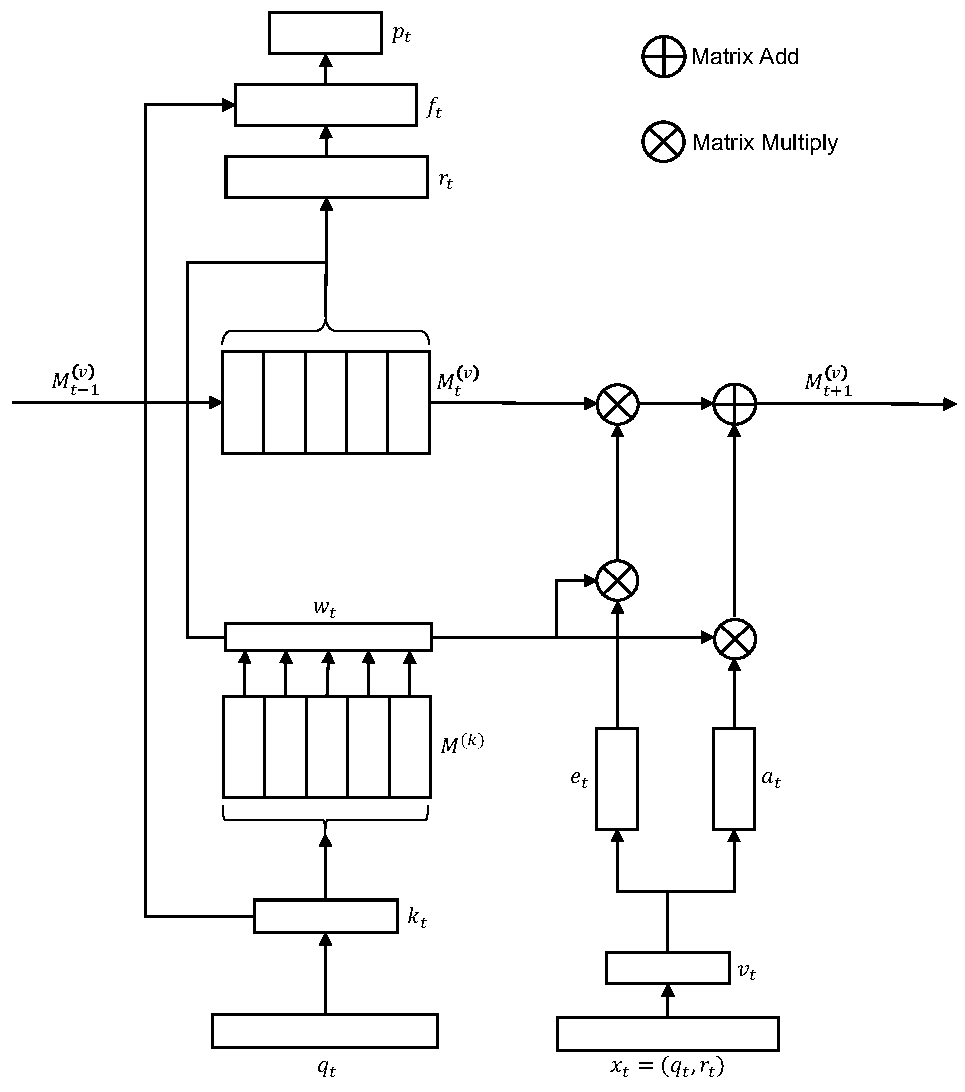
\includegraphics[width=0.9\textwidth]{ch3-dkvmn-model.pdf}
    \caption{The original dynamic key-value memory network model}\label{fig:ch3-dkvmn-model}
\end{figure}

In the reading process, the model weights and calculates the weight vector \(w_t\) with the knowledge point mastery matrix \(M^{(v)}\) to obtain the user's mastery representation vector \(r_t\) for the knowledge point. And \(r_t\) is spliced with the current exercise embedding vector \(k_t\), and \(f_t\) is derived after the full-linked activation layer loses \(Tanh(\cdot)\), which indicates the user's mastery of the exercise. The \(f_t\) goes through a final \(Sigmoid(\cdot)\) activation function to output a predicted probability of answering the exercise correctly \(p_t\). During the writing process, the current actual response performance will impact the student's knowledge acquisition status, which is a re-evaluation process. The current interaction record \(x_t=(q_t,a_t)\) will be used as the input to the model. Its embedding representation \(v_t\) will be used to compute the knowledge reduction vector \(e_t\) and the knowledge increase vector \(a_t\), and the reduction and increase vectors will be weighted with \(w_t\) and act on \(M^{(v)}\) thus realizing the change for the student's knowledge state. The training process is performed by minimizing the cross-entropy loss of \(p_t\) with the true label \(a_t\) of the correctness of the answers to the exercises. The whole model is microscopic and thus can be trained efficiently using stochastic gradient descent.

\section{Proposed Model}

\subsection{Algorithm Overview}
%本节的关键点是对学生的知识追踪,本文提出了一种针对DKVMN的改进型知识追踪网络模型,它在原模型的基础上增加了额外的用户答题特征,并通过图网络来改进知识点掌握度表征存储模块,从而为模型增加知识点间关系表征能力。本模型依然具有习题-知识点关联度计算、读取过程、写入过程和知识网络传播过程和预测过程等多个子模块。其模型框架如图。

The key point of this section is the knowledge tracing of students. In this thesis, an improved knowledge tracing network model for DKVMN was proposed, which adds additional user answer features to the original model and improves the knowledge point mastery representation storage module by graph networks, thus adding inter-knowledge point relationship representation capability to the model. The model still has several sub-modules such as exercise-knowledge point association degree calculation, reading process, writing process and knowledge network propagation process, and prediction process. Its model framework is shown in \figname{\ref{fig:ch3-gkvmn-model}}.

\begin{figure}[htbp!]
    \centering
    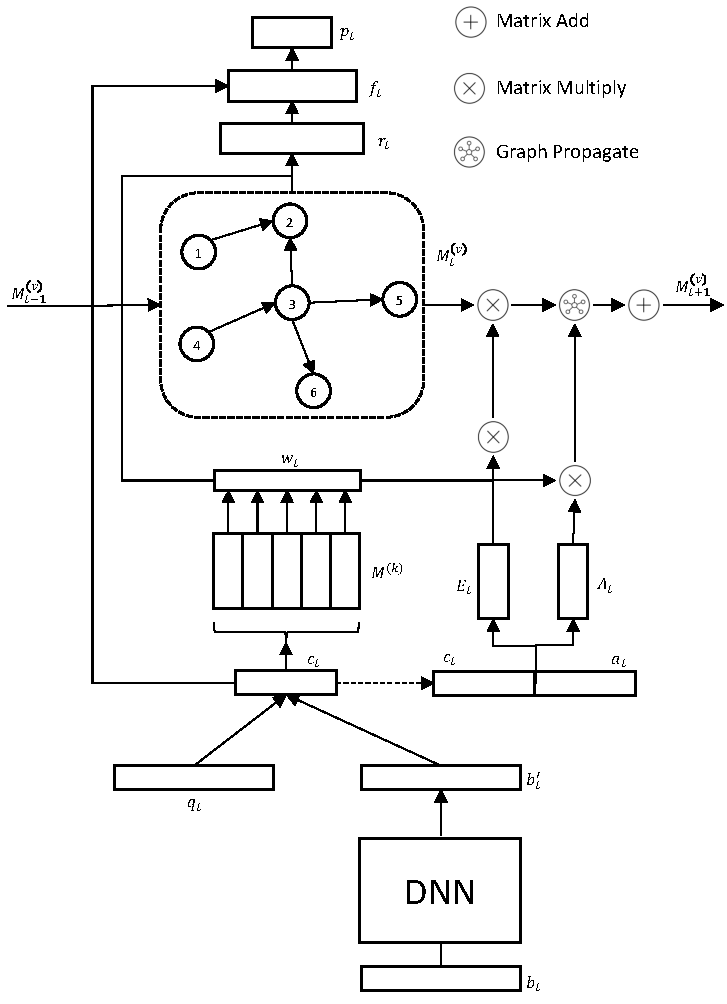
\includegraphics[width=0.9\textwidth]{ch3-gkvmn-model.pdf}
    \caption{The graph key-value memory network architecture}\label{fig:ch3-gkvmn-model}
\end{figure}

\subsection{Student Behavior Capturing}
%在本文中,提出了一种利用DNN来捕捉学生答题特征表征的机制,它与习题特征向量共同形成cross-feature向量,该向量用于后续的习题知识点权重向量计算,它将用户的答题行为特征(例如:是否hint、答题时间、尝试次数)向量\(b_1^t,b_2^t,\ldots,\b_N^t\)输入一个基于多层感知机的特征提取网络中,输出一个对于用户答题能力表征向量\(c_t\)。该向量与原始习题表示向量\(q_t\)进行特征交叉,生成融合用户特征的习题表征向量。具体过程如公式\eqname{\ref{fml:sbcap}}。

In this model, a mechanism is proposed to capture the student's answer feature representation using DNN, which together with the exercise feature vector forms the cross-feature vector that is used for the subsequent calculation of the exercise knowledge point weight vector, which takes the user's answer behavior features (e.g., whether hint, answer time, number of attempts) vector \(b_1^t,b_2^t,\ldots,b_N^t\) into a multilayer perceptron based feature extraction network and outputs a vector \(c_t\) for the user is answering ability representation. This vector is feature-crossed with the original exercise representation vector \(q_t\) to generate an exercise representation vector that incorporates user-related features. The specific process is shown in \eqname{\ref{fml:ch3-sbcap}}. The \(\| \) represents concatenation.

\begin{align}\label{fml:ch3-sbcap}
    \begin{split}
        b^{\prime}_t &= \operatorname{DNN}(b_1^t,b_2^t,\ldots,b_N^t) \\
        c_t &= q_t\|b^{\prime}_t
    \end{split}
\end{align}

%通过这种机制,模型引入了学生的个性化答题特征,从而可以实现对于习题知识点个性化权重计算。它充分利用了神经网络的特征表征能力,抽取出影响学生答题正确性的隐藏因素,从而提高模型整体的可靠性。
Through this mechanism, the model introduces students' personalized answering characteristics, thus enabling the calculation of personalized weights for the exercises' knowledge points. It makes full use of neural networks' feature characterization ability to extract the hidden factors that affect the correctness of students' answers, thus improving the overall reliability of the model.

\subsection{Knowledge-Question Correlation Calculation}
%在学生进行习题练习的过程中,一个习题与多个知识点相关,根据认知诊断理论\cite{chiu2018cognitive},学生对于知识点的掌握程度与学生的内在学习能力决定了学生答题的正确性。与DKVMN类似,本模型用Key矩阵\(M^{(k)}\)来保存习题相关的所有潜在知识点。假设共有\(N^{(K)}\)个知识点,则\(M^{(k)}\in\mathbb{R}^{N^{(K)}}\times d_k\),其中\(d_k\)为知识点表征向量的维度。

In the process of students' exercise practice, an exercise question is associated with multiple knowledge points, shown in \figname{\ref{fig:ch3-kq-relationgraph}}. According to the cognitive diagnosis theory~\cite{chiu2018cognitive}, students' mastery of the knowledge points and students' intrinsic learning ability determine the correctness of their answers. Similar to DKVMN, this model uses the Key matrix \(M^{(k)}\) to keep all potential knowledge points related to the exercises. Suppose there are \(N^{(K)}\) knowledge points, then \(M^{(k)}\in\mathbb{R}^{{N^{(K)}}\times d_k}\), where \(d_k\) is the dimensionality of the knowledge point representation vector.

\begin{figure}[htbp!]
    \centering
    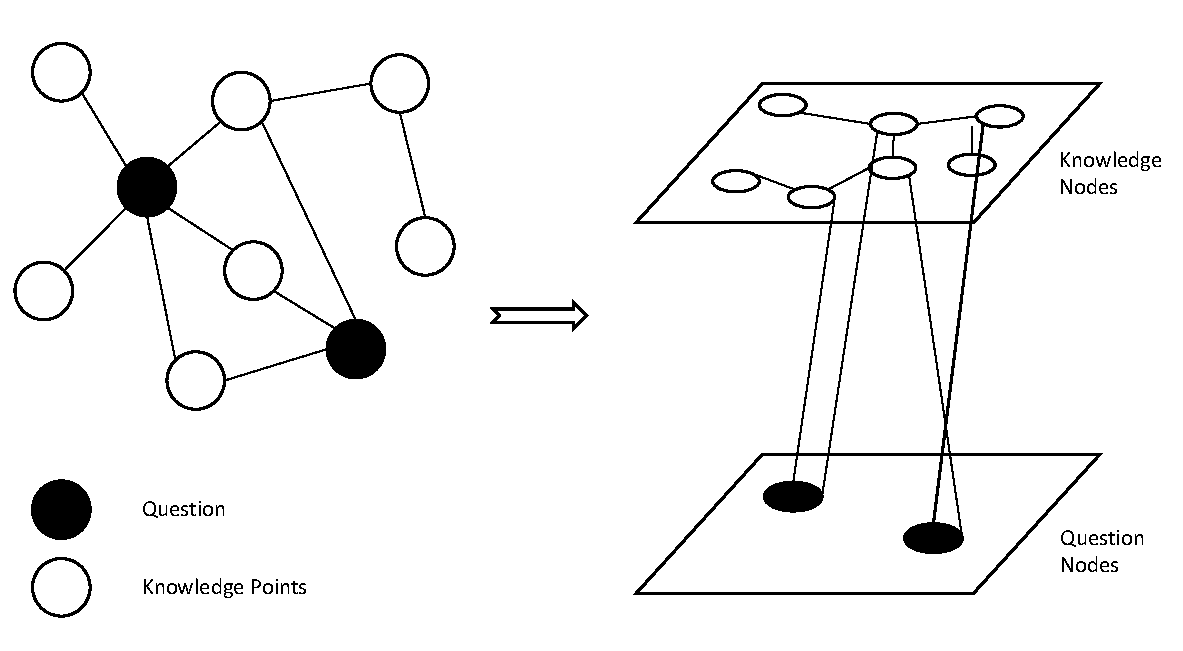
\includegraphics[width=\textwidth]{ch3-kq-relationgraph.pdf}
    \caption{Relation between exercise question and knowledge points}\label{fig:ch3-kq-relationgraph}
\end{figure}
%在\eqname{\ref{fml:sbcap}}中,已经获取了融合学生个性化信息的习题表征向量\(c_t\),其中\(c_t\in\mathbb{R}^{d_k}\),对于第\(i\)个知识点概念,习题与知识点\(i\)的相关度\(w_t(i)\)的计算公式为\eqname{\ref{fml:ch3-corkq}},其中\(\sigma(\cdot)\)为softmax函数。

In \eqname{\ref{fml:ch3-sbcap}}, the exercise representation vector \(c_t\) incorporating students' personalized information has been obtained, where \(c_t\in\mathbb{R}^{d_k}\), and the correlation \(w_t(i)\) between the exercise and the knowledge point \(i\) for the \(i\)th knowledge point concept is calculated by is \eqname{\ref{fml:ch3-corkq}}, where \(\sigma(\cdot)\) is the softmax function.

\begin{align}\label{fml:ch3-corkq}
    \begin{split}
        w_t(i)=\sigma(c_t M^{(k)}(i))
    \end{split}
\end{align}

%由于\(M^{(k)}\)实际上是一个矩阵,因此可以通过矩阵运算来获得总体的相关向量\(\mathbf{w}_t=(w_t(1),w_t(2),\ldots,w_t(N^{(K)}))\)。
Since \(M^{(k)}\) is a matrix, the correlation vector \(\mathbf{w}_t=(w_t(1),w_t(2),\ldots,w_t(N^{(K)}))\) can be obtained by matrix operations like \eqname{\ref{fml:ch3-corkq-mat}}.

\begin{align}\label{fml:ch3-corkq-mat}
    \begin{split}
        \mathbf{w}_t=\sigma(c_t M^{(k)})
    \end{split}
\end{align}

%该向量代表习题与知识点的相关度表征,且经过融合用户的答题特征,能够捕获更多答题行为的影响因素。
The vector \(\mathbf{w}_t\) represents the relation representation of the exercises and knowledge points, and after fusing the user's answer characteristics, it can capture more influencing factors of the answer behavior.

\subsection{Knowledge Mastery Calculation Process}
%本节的目的是计算用户对习题的潜在掌握程度,它是通过计算用户对习题相关知识点的掌握程度来完成。用户对于知识点的掌握程度通过一个矩阵\(M^{(v)}\in\mathbb{R}^{N^{(K)}\times d_v}\)来保存,其中\(d_v\)代表知识点掌握表征向量的维度。该矩阵与DKVMN的区别在于,矩阵会在后续经过图节点信息传播来对相关知识点进行掌握度修改。

The purpose of this section is to calculate the user's potential mastery of the exercise, which is performed by calculating the user's mastery of the knowledge points associated with the exercise. A matrix \ keeps the user's mastery of the knowledge points \((M^{(v)}\in\mathbb{R}^{N^{(K)}\times d_v}\), where \(d_v\) represents the dimensionality of the knowledge point mastery representation vector. The difference between this matrix and DKVMN is that the graph node information propagation will subsequently modify the matrix to the relevant knowledge points in terms of mastery.

%将前一节计算得到的习题与知识点的相关度表征向量\(\mathbf{w}_t\)与当前用户知识点掌握矩阵\(M^{(v)}\)进行加权和计算,如公式\eqname{\ref{}}所示
The correlation representation vector \(\mathbf{w}_t\) of the exercises and knowledge points calculated in the previous section is weighted and calculated with the current user knowledge mastery matrix \(M^{(v)}\), as shown in equation \eqname{\ref{fml:ch3-read}}.

\begin{align}\label{fml:ch3-read}
    \begin{split}
        r_t=\mathbf{w}_t M^{(v)}
    \end{split}
\end{align}

%计算得到的\(r_t\in\mathbb{R}^{d_v}\)表示用户对于习题的掌握程度,该向量考虑了用户的答题特征,相对于DKVMN融合了更多特征。本模型中,读取过程位于图传播计算之前,其目的在于防止图信息重复传播导致的信息增益爆炸。

In the model, the read process is located before the graph propagation calculation, and its purpose is to prevent the information gain explosion caused by repeated propagation of graph information.

\subsection{Knowledge Erase and Add Process with Graph Propagation}
%本节是计算用户在实际答题后,对于知识掌握的重新评估值。本节加入了图传播机制,它考虑了知识点的掌握程度变化引起的相关知识点的熟练度变化。本节的输入是\x_t=(c_t,a_t)\in\mathbb{R}^{(d_k+1)\times d_v}\),其中\(a_t\)是学生对于习题\(q_t\)的回答正确性嵌入表示,它与习题表征向量\(c_t\)共同用于计算答题记录嵌入表征向量\(v_t\),知识掌握增加向量\(A_t\)与知识掌握减少向量\(E_t\)。\(v_t\)的计算公式为\eqname{\ref{fml:ch3-write-vt}}. 
This section calculates the reassessment value of the user's knowledge mastery after actually answering the questions. This section incorporates a graph propagation mechanism, which takes into account the change in the proficiency of the relevant knowledge points caused by the change in the mastery of the knowledge points. The input of this section is \(x_t=(c_t,a_t)\in\mathbb{R}^{(d_k+1)\times d_v} \), where \(a_t\) is the embedded representation of the correctness of students' answers to the exercise \(q_t\), which is used together with the exercise representation vector \(c_t\) to compute the answer record embedding representation vector \(v_t\). the knowledge acquisition increase vector \(A_t\), and the knowledge acquisition decrease vector \(E_t\). The formula for \(v_t\) is \eqname{\ref{fml:ch3-write-vt}}.

\begin{align}\label{fml:ch3-write-vt}
    \begin{split}
        v_t &= \operatorname{Emb}(x_t)
    \end{split}
\end{align}

%知识掌握减少向量\(E_t\in\mathbb{R}^{d_v}\)通过\(v_t\)来计算,它被首先应用于知识掌握矩阵\(M^{(v)}\)。该计算通过加权和的方式完成。权重来自于前文计算得到的习题知识点相关矩阵\(\mathbf{w}_t\),对于第\(i\)个知识点知识掌握减少量\(\Delta{M^{(v)}(i)}_a\)和知识掌握增加量\(\Delta{M^{(v)}(i)}_e\)的计算公式是\eqname{\ref{fml:ch3-write-delta}}。其中\(W^{(e)}\in\mathbb{R}^{d_v \times d_v}\)和\(W^{(a)}\in\mathbb{R}^{d_v \times d_v}\)分别是\(E_t\)和\(A_t\)的转换矩阵,\(b^{(e)}\)和\(b^{(a)}\)分别为对应的偏置量。

The knowledge mastery reduction vector \(E_t\in\mathbb{R}^{d_v}\) is computed by \(v_t\), which is first applied to the knowledge mastery matrix \(M^{(v)}\). This calculation is done by means of a weighted sum. The weights are derived from the exercise knowledge point correlation matrix \(\mathbf{w}_t\) obtained from the previous calculation, and for the \(i\)th knowledge point knowledge mastery decrease \(\Delta_e{M^{(v)}(i)}\) and knowledge mastery increase \(\Delta_a{M^{(v)}(i)}\) are calculated as \eqname{\ref{fml:ch3-write-delta}}, where \(W^{(e)}\in\mathbb{R}^{d_v \times d_v}\) and \(W^{(a)}\in\mathbb{R}^{d_v \times d_v}\) are the transformation matrices of \(E_t\) and \(A_t\), respectively, and \(b^{(e)}\) and \(b^{(a)} \) are the corresponding biases, respectively.

\begin{align}\label{fml:ch3-write-delta}
    \begin{split}
        E_t &= \operatorname{Sigmoid}(W^{(e)}v_t+b^{(e)})\\
        A_t &= \operatorname{Tanh}(W^{(a)}v_t+b^{(a)})\\
        \Delta_e{M^{(v)}_t(i)} & = w_t(i) E_t \\
        \Delta_a{M^{(v)}_t(i)} & = w_t(i) A_t
    \end{split}
\end{align}

%在进行知识掌握熟练度更改时,先将原始的知识掌握向量的每个key slot与\(\Delta_e{M^{(v)}(i)}\)进行加权减法,然后加上知识掌握增益\Delta_a{M^{(v)}(i)} \如公式所示。

For the knowledge mastery proficiency change, each key slot of the original knowledge mastery vector is first weighted and subtracted from \(\Delta_e{M^{(v)}(i)}\), and then the knowledge mastery gain \(\Delta_a{M^{(v)}(i)}\) is added as shown in \eqname{\ref{fml:ch3-modify}}.

\begin{align}\label{fml:ch3-modify}
    \begin{split}
        \tilde{M^{(v)}_t}(i) &= M^{(v)}(i)(1-\Delta_e{M^{(v)}(i)}) \\
        \tilde{M^{(v)}_{t+1}}(i) &= \tilde{M^{(v)_t}}(i) + \Delta_a{M^{(v)}_t(i)}
    \end{split}
\end{align}

%最后,每个知识点的变化会对相邻知识点产生影响,因此此处引入了图网络传播机制,对整个知识掌握矩阵进行值重新分布。类似于图卷积神经网络的网络传播机制,则有公式\eqname{\ref{fml:ch3-graphpropagate}}。其中\(\tilde{M^{(v)}_{t+1}}(i))\in\mathbb{R}^{N^{(K)}\times d_v}\)为图网络的上一层和输入。\(M^{(v)}_{t+1}(i)\)为图网络的下一层。\(\tilde{A}=A+I_{N^{(K)}}\)为自连接邻接矩阵。\(\tilde{D}\)为度矩阵,即\(\tilde{D}_ii=\sum_j{\tilde{A}_ij}\),\(W_t\in\mathbb{R}^{d_v \times d_v}\)为待训练的权重矩阵。\(\sigma(\cdot)\)为激活函数,在此处使用\(LeakyReLU(\cdot)\)。

Finally, changes in each knowledge point have an impact on neighboring knowledge points, so a graph network propagation mechanism is introduced here to redistribute the values across the knowledge mastery matrix. Similar to the network propagation mechanism of graph convolutional neural network, then there is the formula \eqname{\ref{fml:ch3-graphpropagate}}, where \(\tilde{M^{(v)}_{t+1}}(i)\in\mathbb{R}^{N^{(K)}\times d_v}\) is the upper layer of the graph network and the input. \(M^{(v)}_{t+1}(i)\) is the next layer of the graph network. \(\tilde{A}=A+I_{N^{(K)}}\) is the self-connected adjacency matrix. \(\tilde{D}\) is the degree matrix, i.e. \(\tilde{D}_{ii}=\sum_j{\tilde{A}_{ij}}\), \(W_t\in\mathbb{R}^{d_v \times d_v}\) is the matrix of weights to be trained. \(\sigma(\cdot)\) is the activation function, and \(LeakyReLU(\cdot)\) is used here.

\begin{align}\label{fml:ch3-graphpropagate}
    M^{(v)}_{t+1}(i) \leftarrow \sigma(\tilde{D}^{-\frac{1}{2}}\tilde{A}\tilde{D}^{\frac{1}{2}}\tilde{M^{(v)}_{t+1}}(i)W_t)
\end{align}

%由此可见,知识点的邻接矩阵是图传播的关键,本文提出了基于统计的方式来计算知识点邻接矩阵\(A\),即当知识点\(i,j\)共现次数超过某一阈值时,将\(i,j\)知识点设置为相关。如公式\eqname{\ref{fml:ch3-confidence}}所示。

It can be seen that the adjacency matrix of knowledge points is the key to graph propagation, and this thesis proposes a statistical-based approach to calculate the knowledge point adjacency matrix \(A\), i.e. when the number of co-occurrences of knowledge points \(i,j\) exceeds a certain threshold, \(i,j\) knowledge points are set to be relevant. As shown in equation \eqname{\ref{fml:ch3-confidence}}, the \(P_{ij}\) represents the probability that exercise \(i\) and exercise \(j\) exist in one exercise.
\begin{align}\label{fml:ch3-confidence}
    A_{ij}=\{\begin{array}{ll}
        0, & \text{ if } P_{ij}<\tau^{(k)}      \\
        1, & \text{ if } P_{ij} \geq \tau^{(k)}
    \end{array}
\end{align}


Finally, changes in each knowledge point have an impact on neighboring knowledge points, so a graph network propagation mechanism is introduced here to redistribute the values across the knowledge mastery matrix.


% \subsubsection{Statistics-based Method}


% \subsubsection{Multi-head Attention Based}


\subsection{Prediction}
%经过计算得到的知识点掌握熟练度表征\(r_t\)可以用于计算习题回答正确的概率。它通过中间和向量\(f_t\)来计算,其中\(f_t\)包含了习题相关知识点的掌握程度和习题本身的信息。计算公式如\eqname{\ref{fml:ch3-predicting-function-f}}}所示,其中权重转移矩阵\(W_f\)和偏置向量\(b_f\)为待训练参数。
The computed knowledge point mastery proficiency representation \(r_t\) can be used to calculate the probability of answering the exercise correctly. It is calculated by the intermediate sum vector \(f_t\), where \(f_t\) contains information about the mastery of the knowledge points related to the exercise and the exercise itself. The calculation formula is shown in \eqname{\ref{fml:ch3-predicting-function-f}}, where the weight transfer matrix \(W_f\) and the bias vector \(b_f\) are the parameters to be trained.
\begin{align}\label{fml:ch3-predicting-function-f}
    f_t = \operatorname{Tanh}(W_f^T[r_t,c_t] + b_f)
\end{align}

%然后经过一个全连接激活层,输出对于习题\(q_t\)的正确性预测\(p_t\)。计算公式如\eqname{\ref{fml:ch3-predicting-function-p}},其中权重转移矩阵\(W_p\)和偏置向量\(b_p\)为待训练参数。
Then after a fully connected activation layer, the correctness prediction \(p_t\) for the exercise \(q_t\) is output. The formula is calculated as \eqname{\ref{fml:ch3-predicting-function-p}}, where the weight transfer matrix \(W_p\) and the bias vector \(b_p\) are the parameters to be trained.
\begin{align}\label{fml:ch3-predicting-function-p}
    p_t = \operatorname{Sigmoid}(W_p^T f_t + b_p)
\end{align}

%整个网络通过端到端的训练来进行,真实的正确性为\(a_t\),整体的损失函数为
The whole network is trained in an end-to-end manner j with true correctness \(a_t\), and the overall loss function is \eqname{\ref{fml:ch3-loss}}.
\begin{align}\label{fml:ch3-loss}
    \mathcal{L} = -\sum\limits_{t}{(a_t\log(p_t)+(1-a_t)\log(1-p_t))}
\end{align}


\subsection{Knowledge Mastery}
Due to the nature of GKVMN, the knowledge mastery \(M^{(v)}\) is explicit so that it can be directly used as a kind of recommendation system for judgment. Moreover, it can be subsequently used as a student knowledge mastery state analysis.

\section{Experiments}
%本节中,通过多个专用的知识追踪数据集来investigate提出的模型性能,与目前已经提出的Baseline模型进行性能对比。本章先对所用到的数据集进行介绍和统计,然后提出用于模型性能对比的度量标准、实验设置和运行参数环境等,最后得出结果并进行分析。
In this section, algorithms, including the performance, are investigated through multiple dedicated knowledge tracing data sets, and the performance of the proposed baseline model is compared. This chapter first introduces and counts the data sets used, then proposes metrics, experimental settings, and operating parameter environments for model performance comparison, and finally draws the results and analyzes them.

\subsection{Datasets}
After investigating the existing knowledge tracing model, the thesis selected the more popular ASSISTment data set and Statics data set related to mathematics, preprocessed the data set, cleaned the data, obtained the training set, and performed the performance with the Baseline model Compared.
%本实验主要采用ASSISTment2009数据集用于测试,该数据集是在2009-2010学年于ASSISTment教学平台上采集的真实教育数据。该数据集包含一个Skill builder问题集合,当学生达到一定的标准时,即被认为是掌握了某个技能。当学生掌握某个技能后,将不会有关于该技能的习题推送。

The experiment was conducted using the ASSISTment 2009 dataset, which is a collection of real educational data collected on the ASSISTment teaching platform during the 2009-2010 academic year. The dataset contains a set of Skill builder questions, where students are considered to have mastered a skill when they meet specific criteria. Once a student has mastered a skill, there will be no exercises pushed for that skill.


\subsubsection{Data Description}
%在该数据集的基础记录中,每一行为一个问题的答题记录,包含一系列的特征,例如问题的Id表示problem_id,学生的ID表示user_id,学生的答题次数attempt_count,学生答题用时ms_first_response,问题的相关技能ID表示skill_id等,具体的描述如下:

In the base record of this dataset, each row is a question answering record, containing a series of features, such as problem\_id, user\_id, attempt\_count, ms\_first\_response skill\_id, etc. The specific description is as \tblname{\ref{tbl:ch3-assist2009-heading}}.

\begin{table}[htbp!]
    \centering
    \caption{The column heading of ASSISTment Dataset}\label{tbl:ch3-assist2009-heading}
    \begin{tabular}{lc}
        \toprule
        column heading & description                                                       \\
        \midrule
        problem\_id    & problem or exercise ID                                            \\
        user\_id       & the ID of the user                                                \\
        correct        & a binary value, 1 represents correct while 0 represents incorrect \\
        attempt\_count & Number of student attempts on the exercise                        \\
        skill\_id      & skill ID associated with the exercise                             \\
        hint\_count    & Number of student attempts on this problem                        \\
        first\_action  & The Whether or not the student asks for all hints                 \\
        hint\_total    & Number of possible hints on this problem.                         \\
        \bottomrule
    \end{tabular}
\end{table}

%经过统计,数据集的一些基本统计数据如下
The statistical information of the dataset ASSISTment 2009 after data pre-processing is shown in the \tblname{\ref{tbl:ch3-assist2009-stat}}.
\begin{table}
    \centering
    \caption{Statistics of ASSISTment 2009 dataset}\label{tbl:ch3-assist2009-stat}
    \begin{tabular}{ccccc}
        \toprule
        Statistics      & \makecell[c]{Number                          \\ of Students} & \makecell[c]{Number                         \\of Skills }& \makecell[c]{Number                         \\of Questions }& \makecell[c]{Number                         \\ of Records} \\
        \midrule
        ASSISTment 2009 & 4,032               & 124 & 17,748 & 459,092 \\
        \bottomrule
    \end{tabular}
\end{table}
% Total number of students: 4032
% Training set size: 2580
% Validation set size: 645
% Testing set size: 806
% Number of skills: 123
% Number of features in the input: 246

\subsubsection{Data Preprocessing}
%数据预处理是进行模型训练的重要前置步骤。在原始数据中,部分关键的特征出现了缺失,因此应当首先进行数据清洗,清除这些行。例如:缺失关键的skill\_id,correctness和user\_id的行会被剔除。由于知识追踪等任务是基于个体层面进行,因此一个知识追踪的输入序列必须属于同一个用户。而在原始数据集中,这样的序列是乱序的,因此需要对用户的答题序列基于用户个体做聚合排序处理。为了将答题的正确性融入到特征,需要进行特征交叉,在此处的特征交叉是将skill_id与correct两个特征进行加权相加和平移来进行。特征交叉可以为模型带来非线性。
Data preprocessing is an important antecedent step to perform model training. Some key features are missing in the raw dataset, so data cleaning should be performed first to remove these rows. For example, rows missing the key skill\_id, correctness, and user\_id will be excluded. Since knowledge tracing is performed on an individual level, the input sequence of knowledge tracing must belong to the same user. In the original dataset, such sequences are disordered, so it is necessary to perform aggregated sorting of the user's answer sequences based on individual users. In order to incorporate the correctness of the answers into the new features, feature crossover is required, where the feature crossover is performed by weighting the two features, skill\_id and correct, by summing and translating them. Feature crossing can introduce nonlinearity into the model.
% \begin{itemize}
%     \item problem\_id: problem or exercise ID.\
%     \item user\_id: the ID of the user.
%     \item correct: a binary value, 1 represents correct while 0 represents incorrect.
%     \item attempt_count:
% \end{itemize}

%本实验设置了最长训练序列长度作为超参数,因此对于超过最长训练序列的输入序列,需要进行分割。
In this experiment, the length of the longest training sequence is set as the hyperparameter, so for the input sequence that exceeds the longest training sequence, segmentation is required.
%(1)ASSISTment 2015 是一个用于预测学生考试表现的数据集,它由一系列包含若干知识点标签的问题以及一些学生的答题记录组成。它在2015年于线上教育平台上采集而成。经过数据过滤获得包含19917个学生,约102千个问题,100个知识点标签和约709次交互的数据集。
%(2)ASSISTment 2017 来源于2017年举办的ASSISTments Longitudinal Data Mining Competition。经过数据预处理和数据过滤,数据集包含1709个学生,4117个问题,102个知识点和约943千次交互。
%(3)Statics 2011 数据集来源于统计学课程的答题记录。

\subsubsection{Data Analysis}
%在进行模型训练之前,针对数据集进行因果分析,来筛选出合理的变量作为模型输入可以有效提高模型性能。在本节,从经过预处理的原始数据,选取出可能对最终产生影响的若干特征,进行可视化分析。然后选择合适的特征进行输入。
Before model training, a dependent variable analysis is performed for the dataset to filter out reasonable variables as model inputs can effectively improve model performance. In this section, several features that may impact the final are selected for visualization and analysis from the preprocessed raw data. The appropriate features are then selected for input.
%首先,可以对原数据源进行列相关度分析,获取各个输入特征与输出结果标签的相关度。绘制的列相关度热力图如图所示。可见是与习题答题正确性最相关的几个特征。因此本实验将这些特征作为用户的行为特征加入模型。
First, column correlation analysis can be performed on the original data source to obtain each input feature's correlation with the output result labels. The plotted column correlation heat map is shown in \figname{\ref{fig:ch3-dataset-heatmap}}.

\begin{figure}[htb]
    \centering
    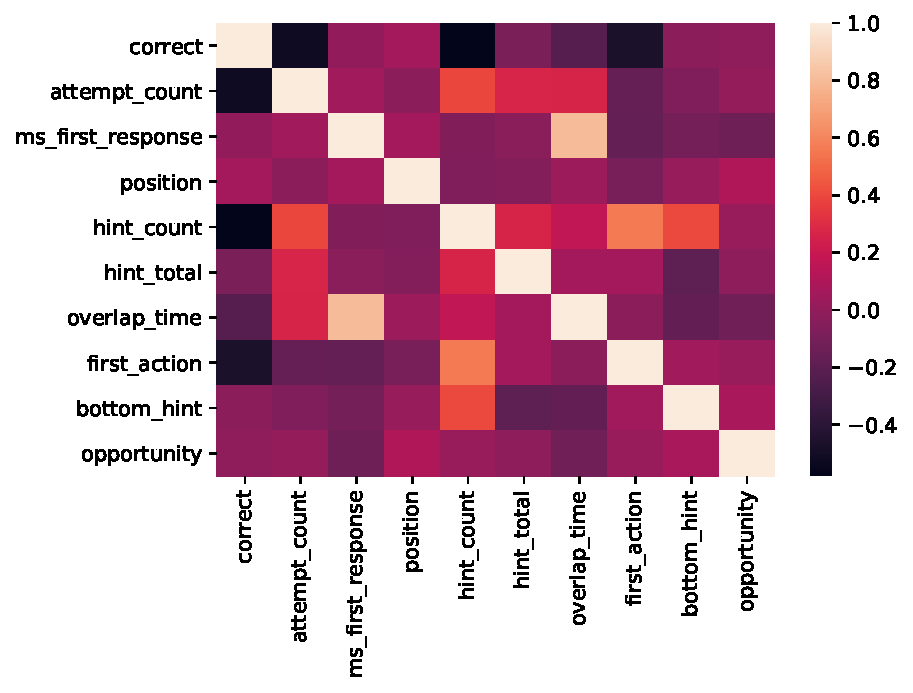
\includegraphics[width=0.85\textwidth]{ch3-dataset-heatmap.pdf}
    \caption{The heat map of original dataset ASSISTment 2009}\label{fig:ch3-dataset-heatmap}
\end{figure}

%然后,结合热力图,分别对筛选出来的特征绘制互相关性图与分布图,得到. 由此可见,这些特征存在一定的互相关性。
Then, combined with the heat map, the mutual correlation map and distribution map are plotted for the filtered features, respectively. The figure is \figname{\ref{fig:ch3-dataset-corrplot}}. It can be seen that there is a certain mutual correlation between these features.
\begin{figure}[htbp!]
    \centering
    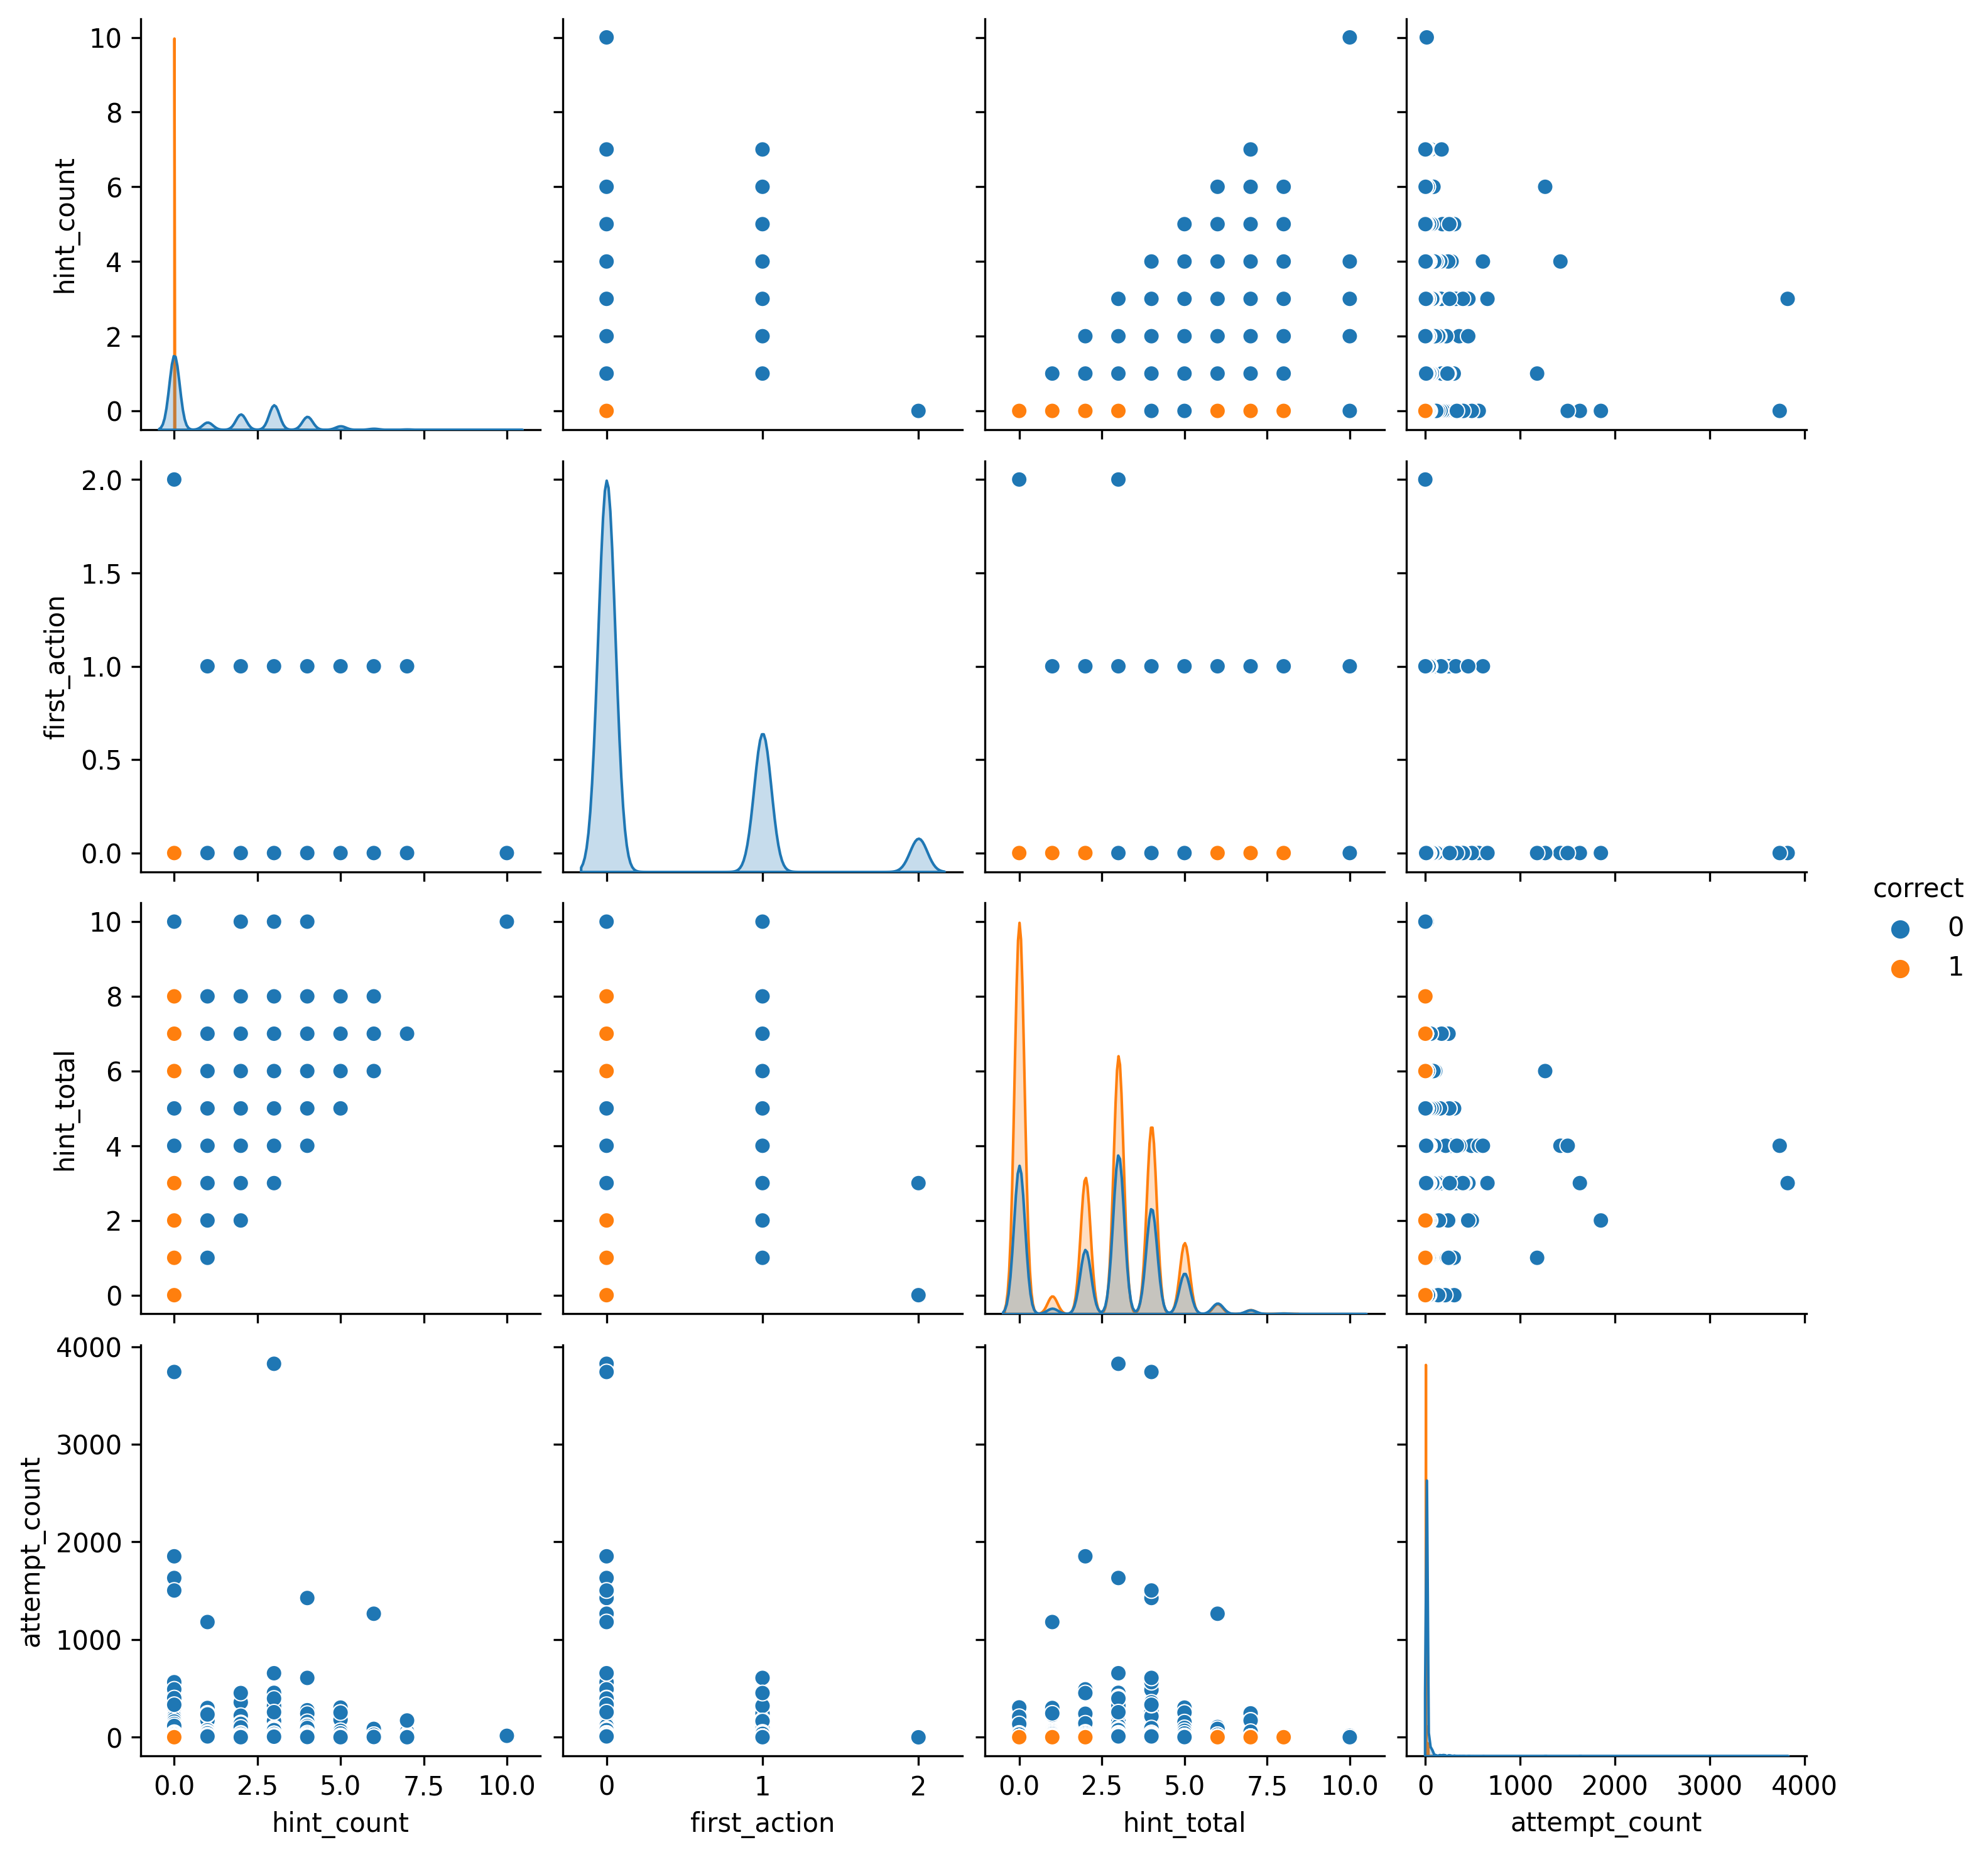
\includegraphics[width=1.0\textwidth]{ch3-dataset-corrplot.png}
    \caption{The correlation plot between features and correctness}\label{fig:ch3-dataset-corrplot}
\end{figure}


%接下来,将每个特征与答题正确性分别绘制互相关图,分析各个特征与目标特征的关系。
Next, each feature was plotted separately against the correctness of the answer, and the relationship between each feature and the target feature was analyzed, as shown in \figname{\ref{fig:ch3-jointplot-hc}} to \figname{\ref{fig:ch3-jointplot-atc}}.

\begin{figure}[htb]
    \centering
    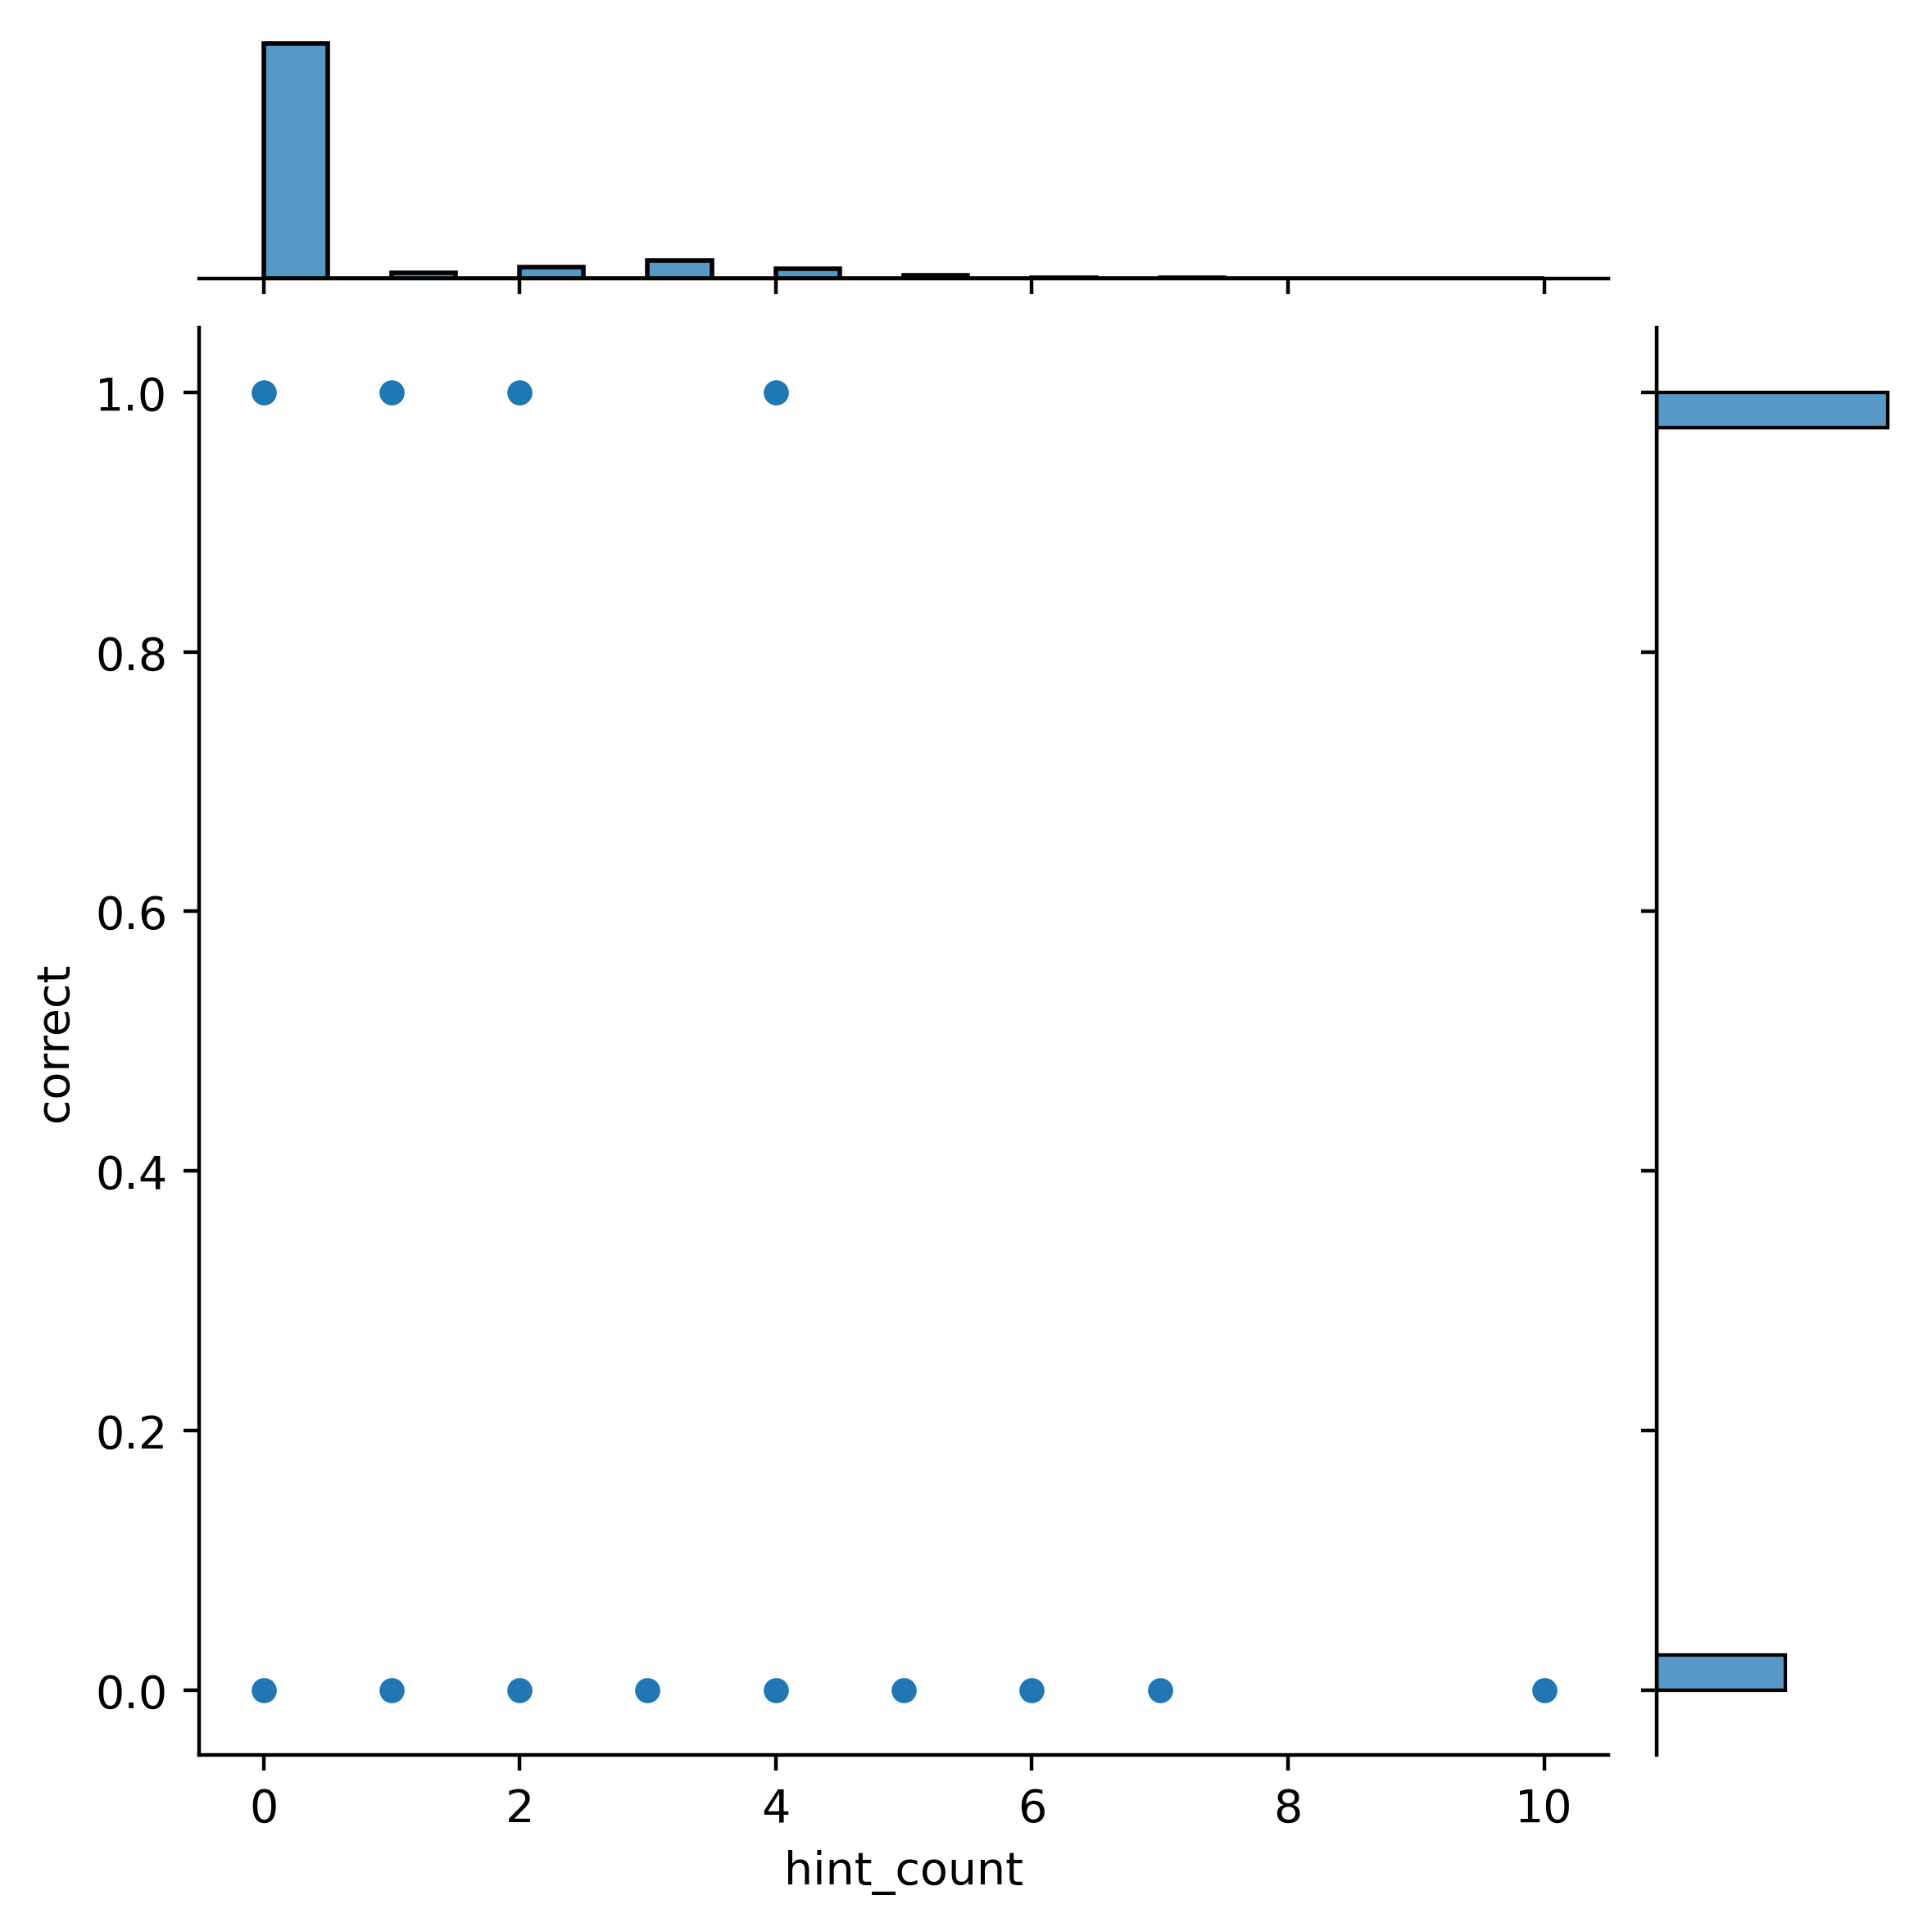
\includegraphics[width=0.85\textwidth]{ch3-jointplot-hc.png}
    \caption{The joint plot of hint\_count}\label{fig:ch3-jointplot-hc}
\end{figure}

\begin{figure}[htb]
    \centering
    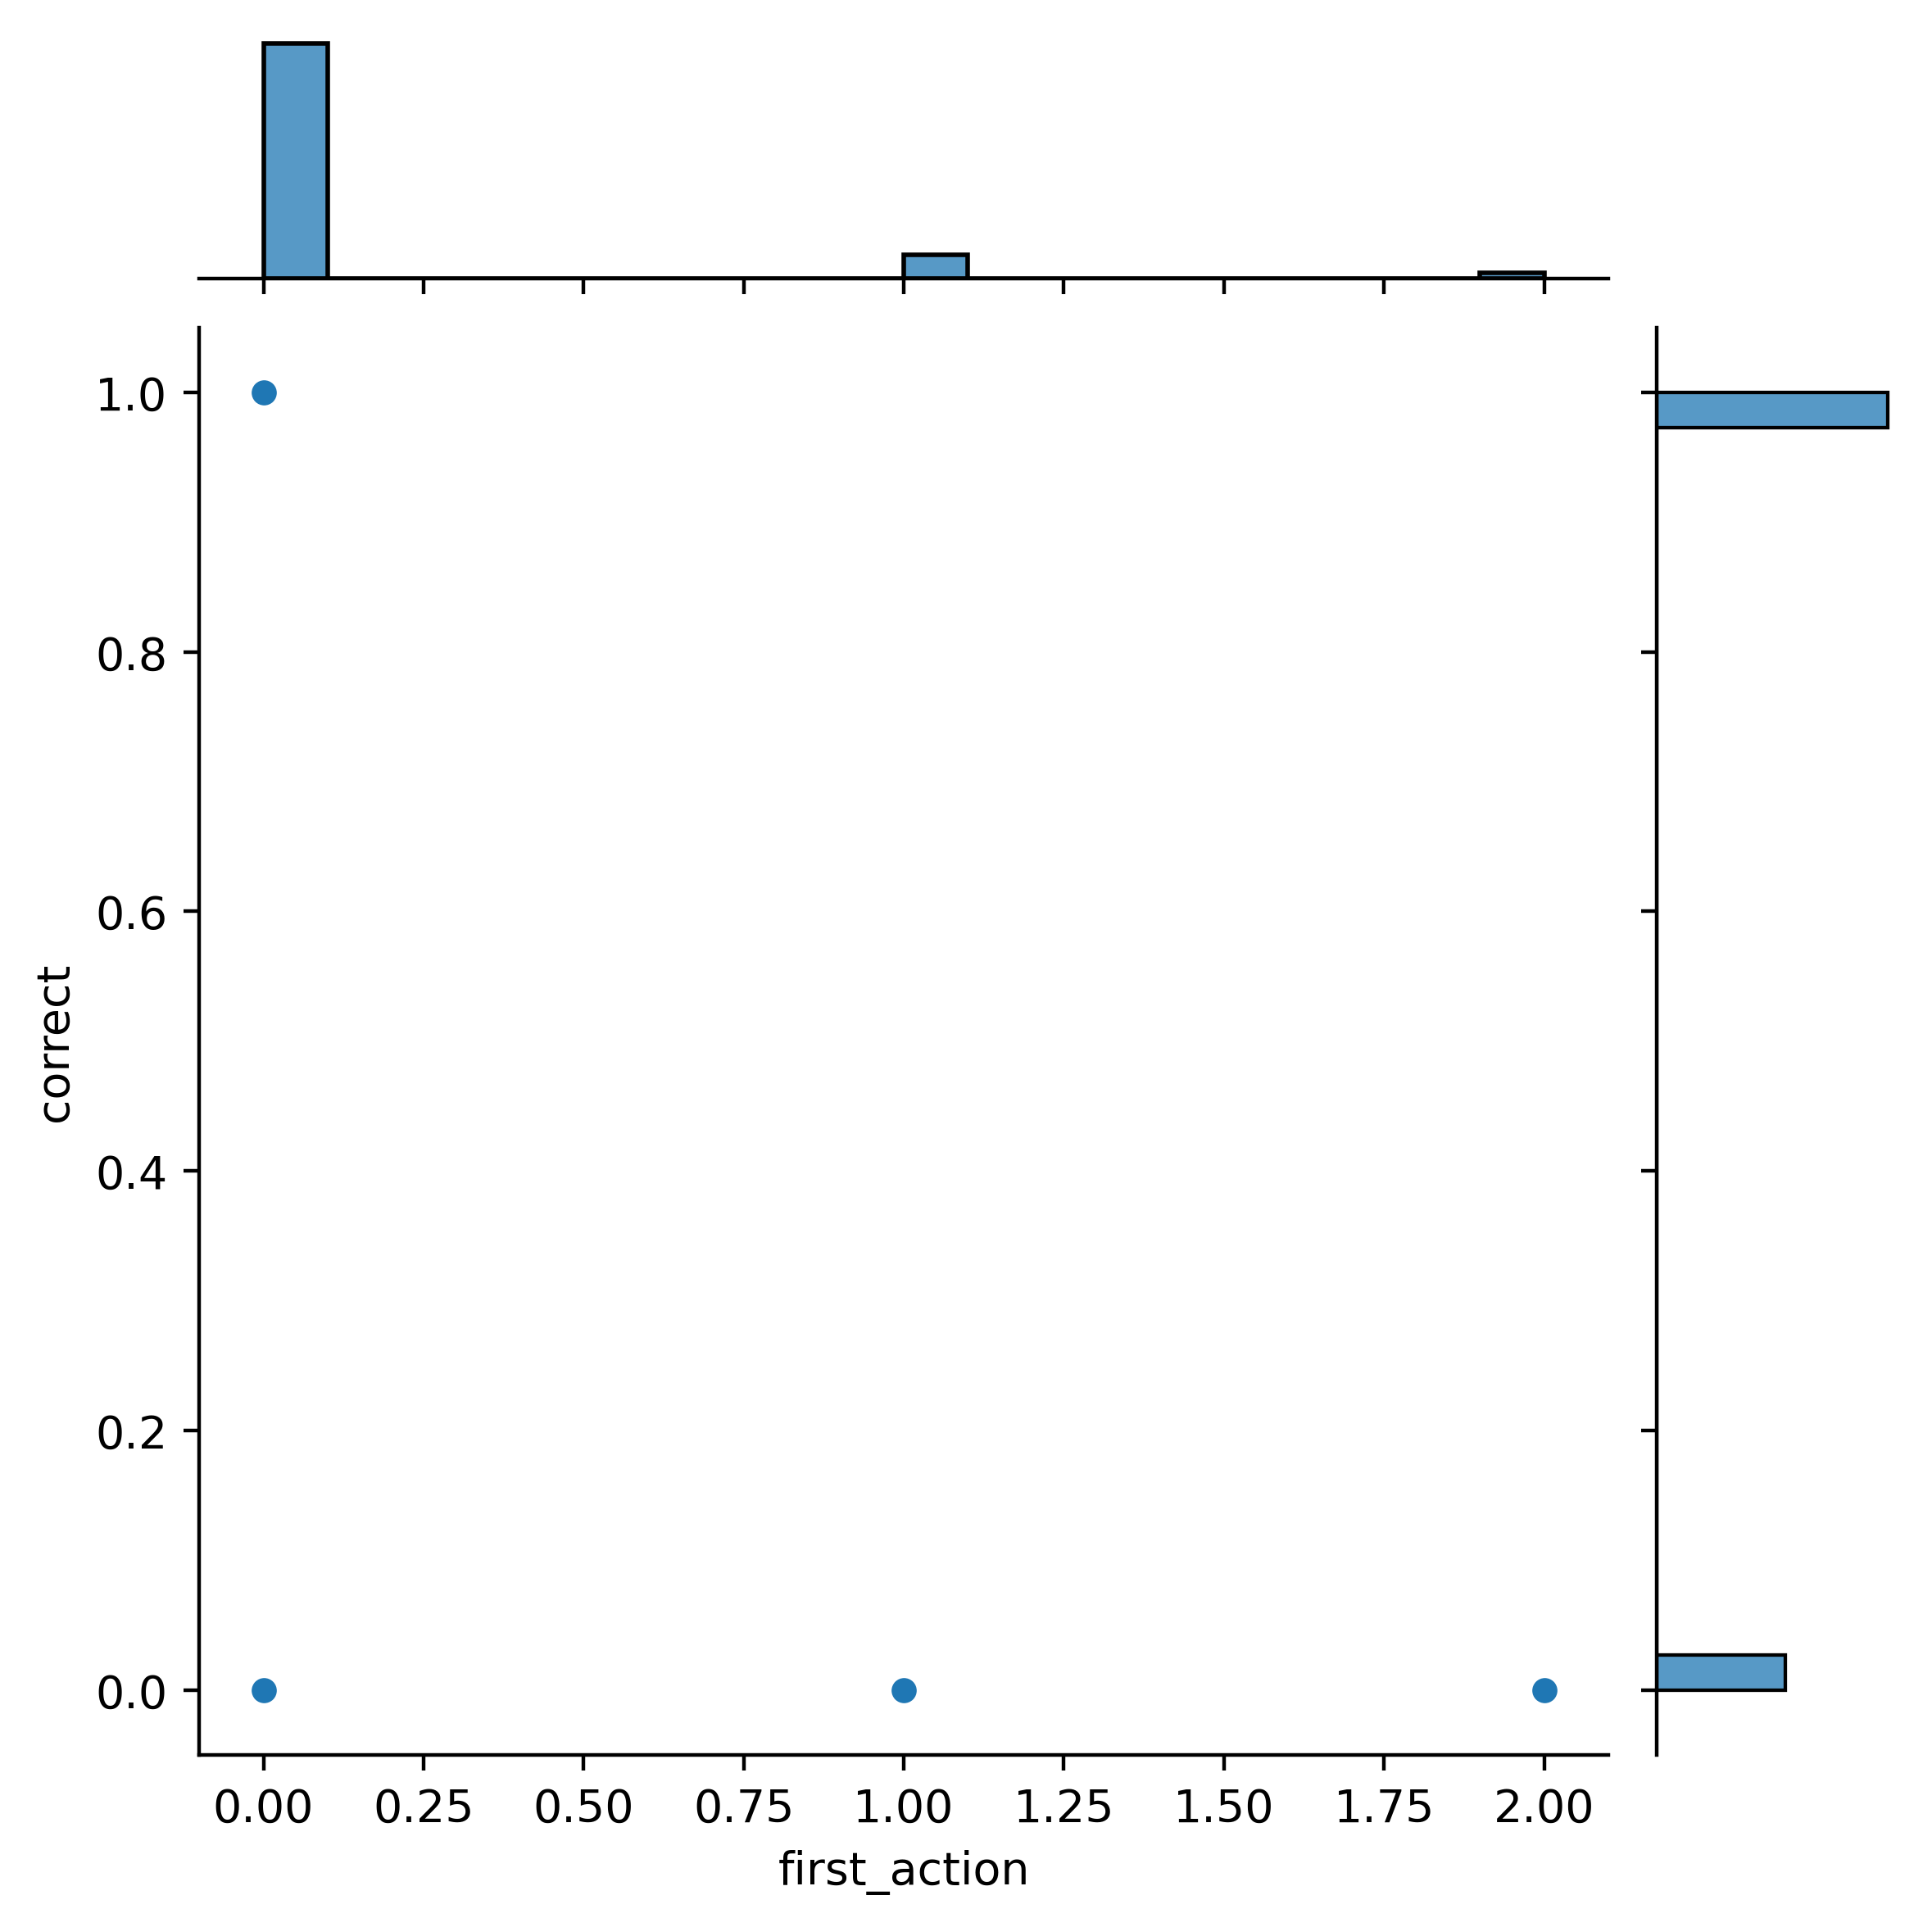
\includegraphics[width=0.85\textwidth]{ch3-jointplot-fc.png}
    \caption{The joint plot of first\_action}\label{fig:ch3-jointplot-fc}
\end{figure}

\begin{figure}[htb]
    \centering
    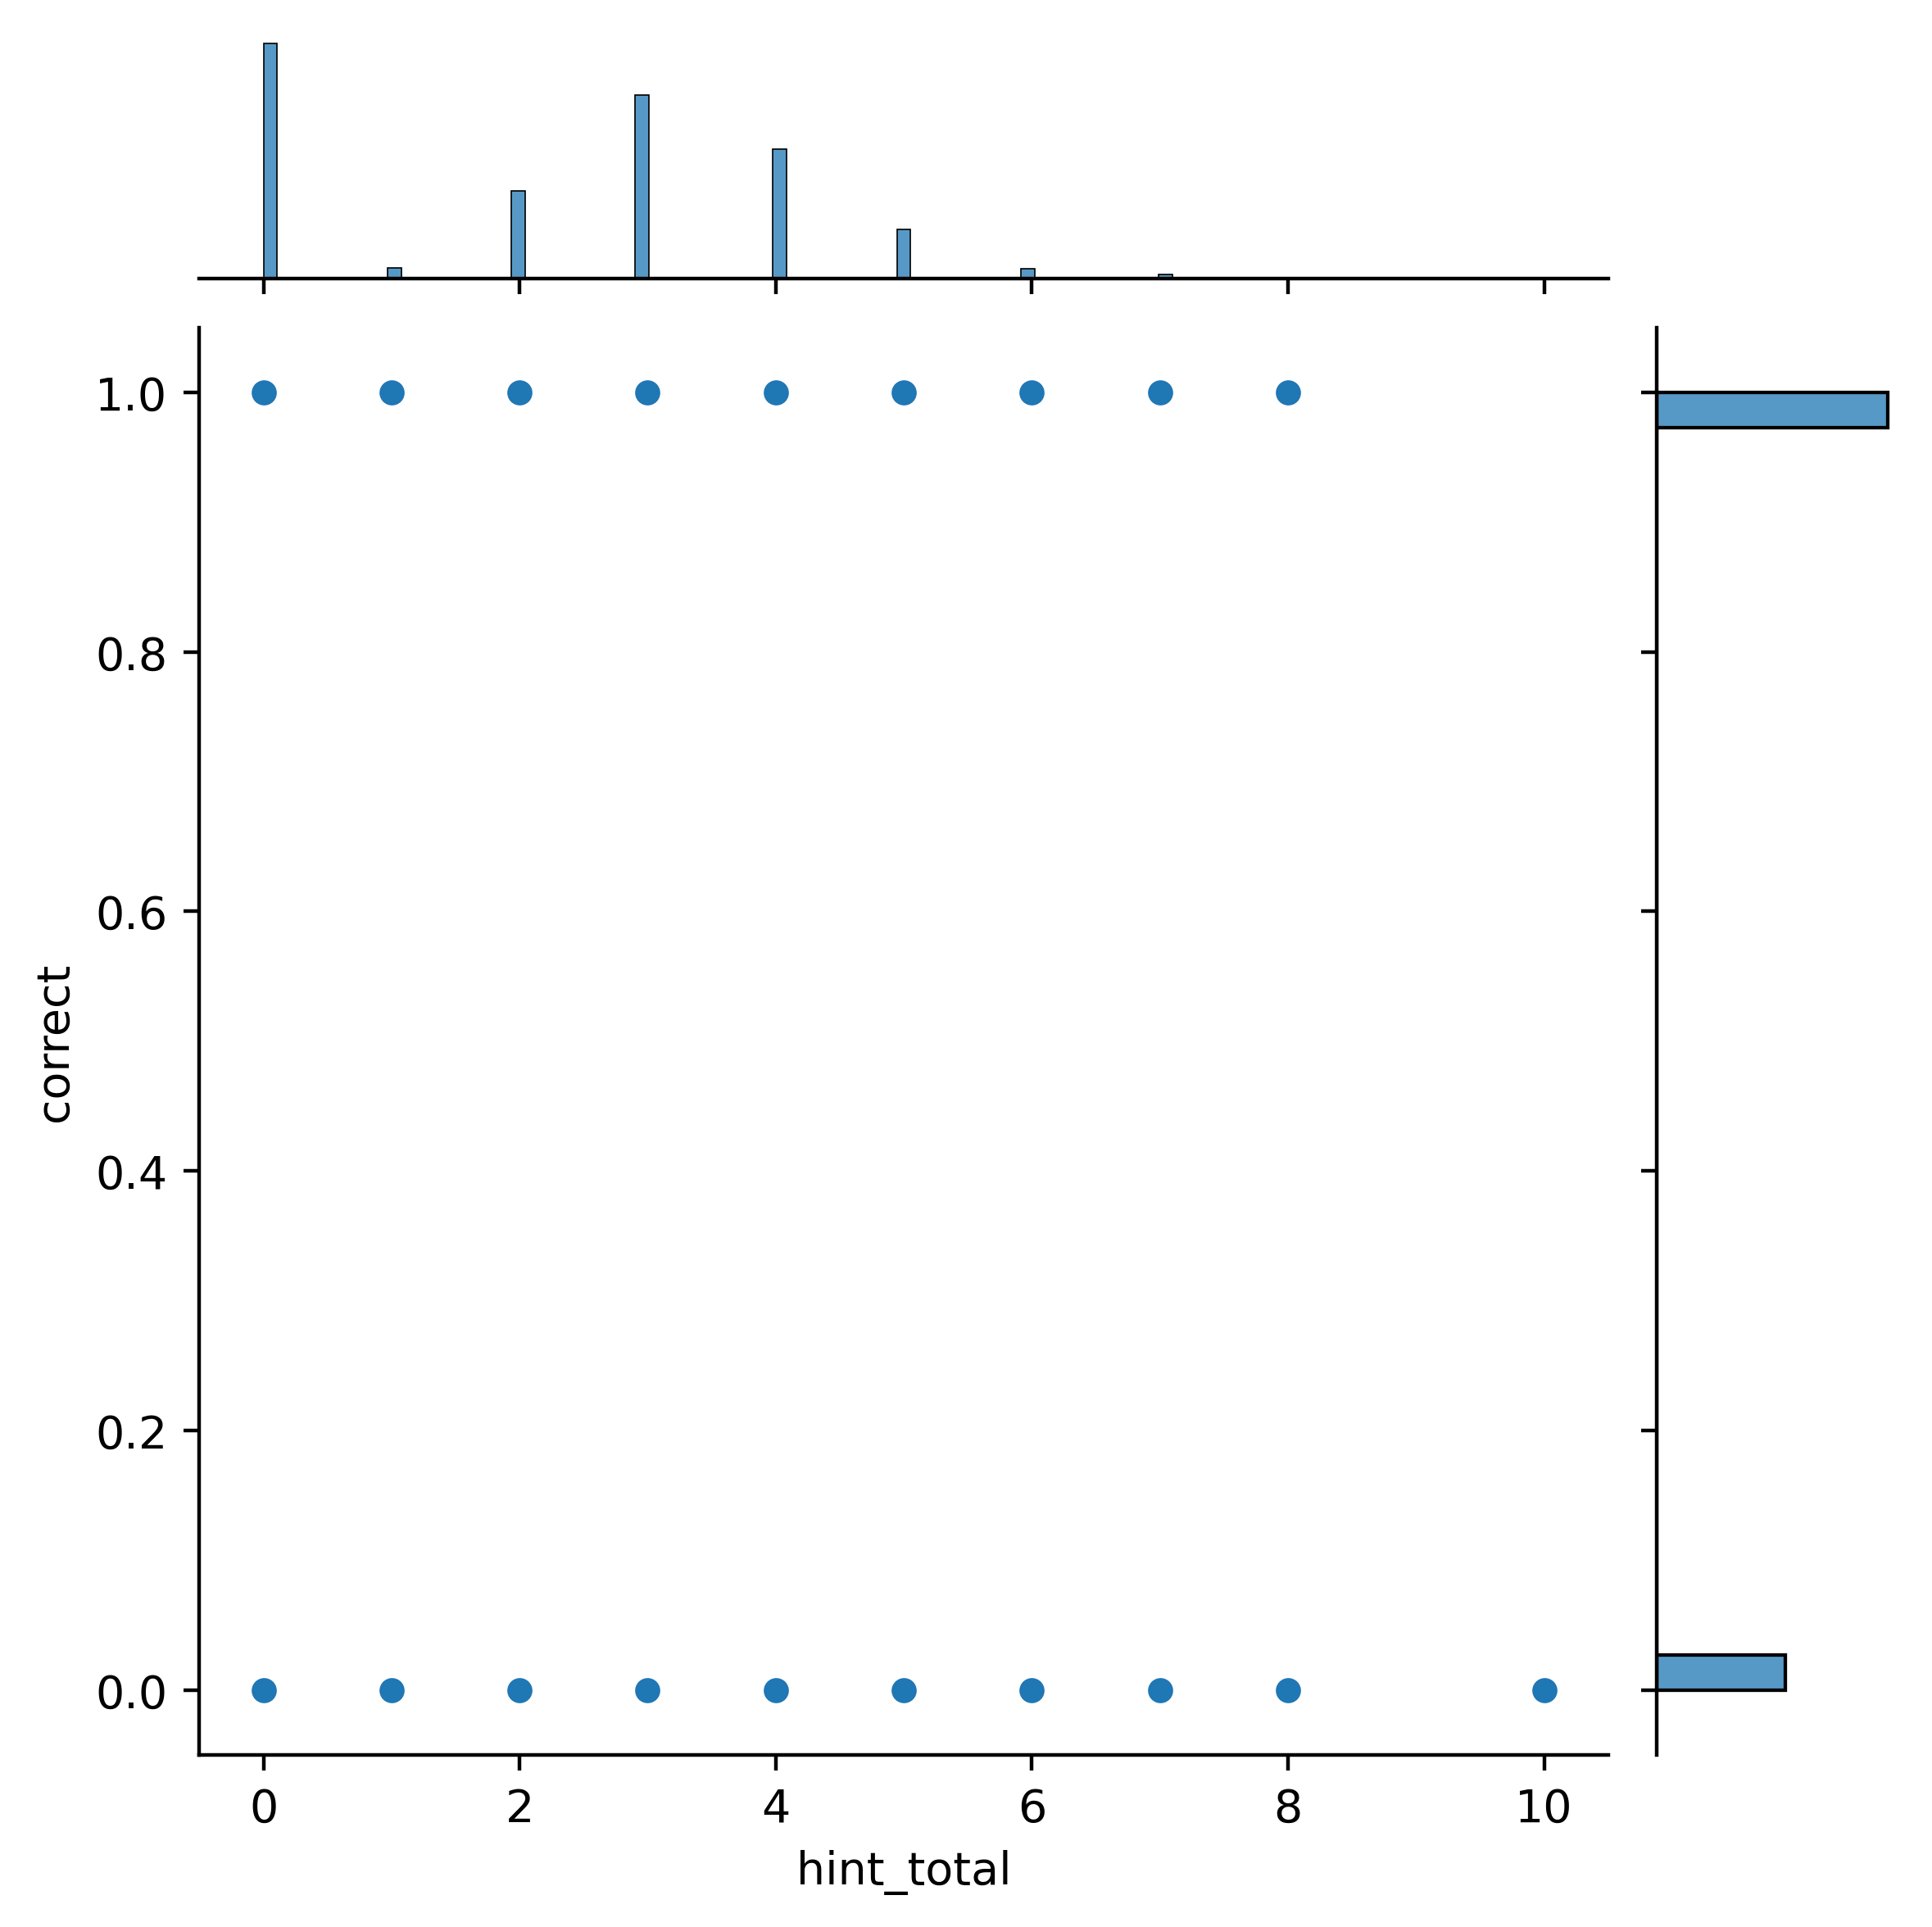
\includegraphics[width=0.85\textwidth]{ch3-jointplot-htc.png}
    \caption{The joint plot of hint\_total}\label{fig:ch3-jointplot-htc}
\end{figure}

\begin{figure}[htb]
    \centering
    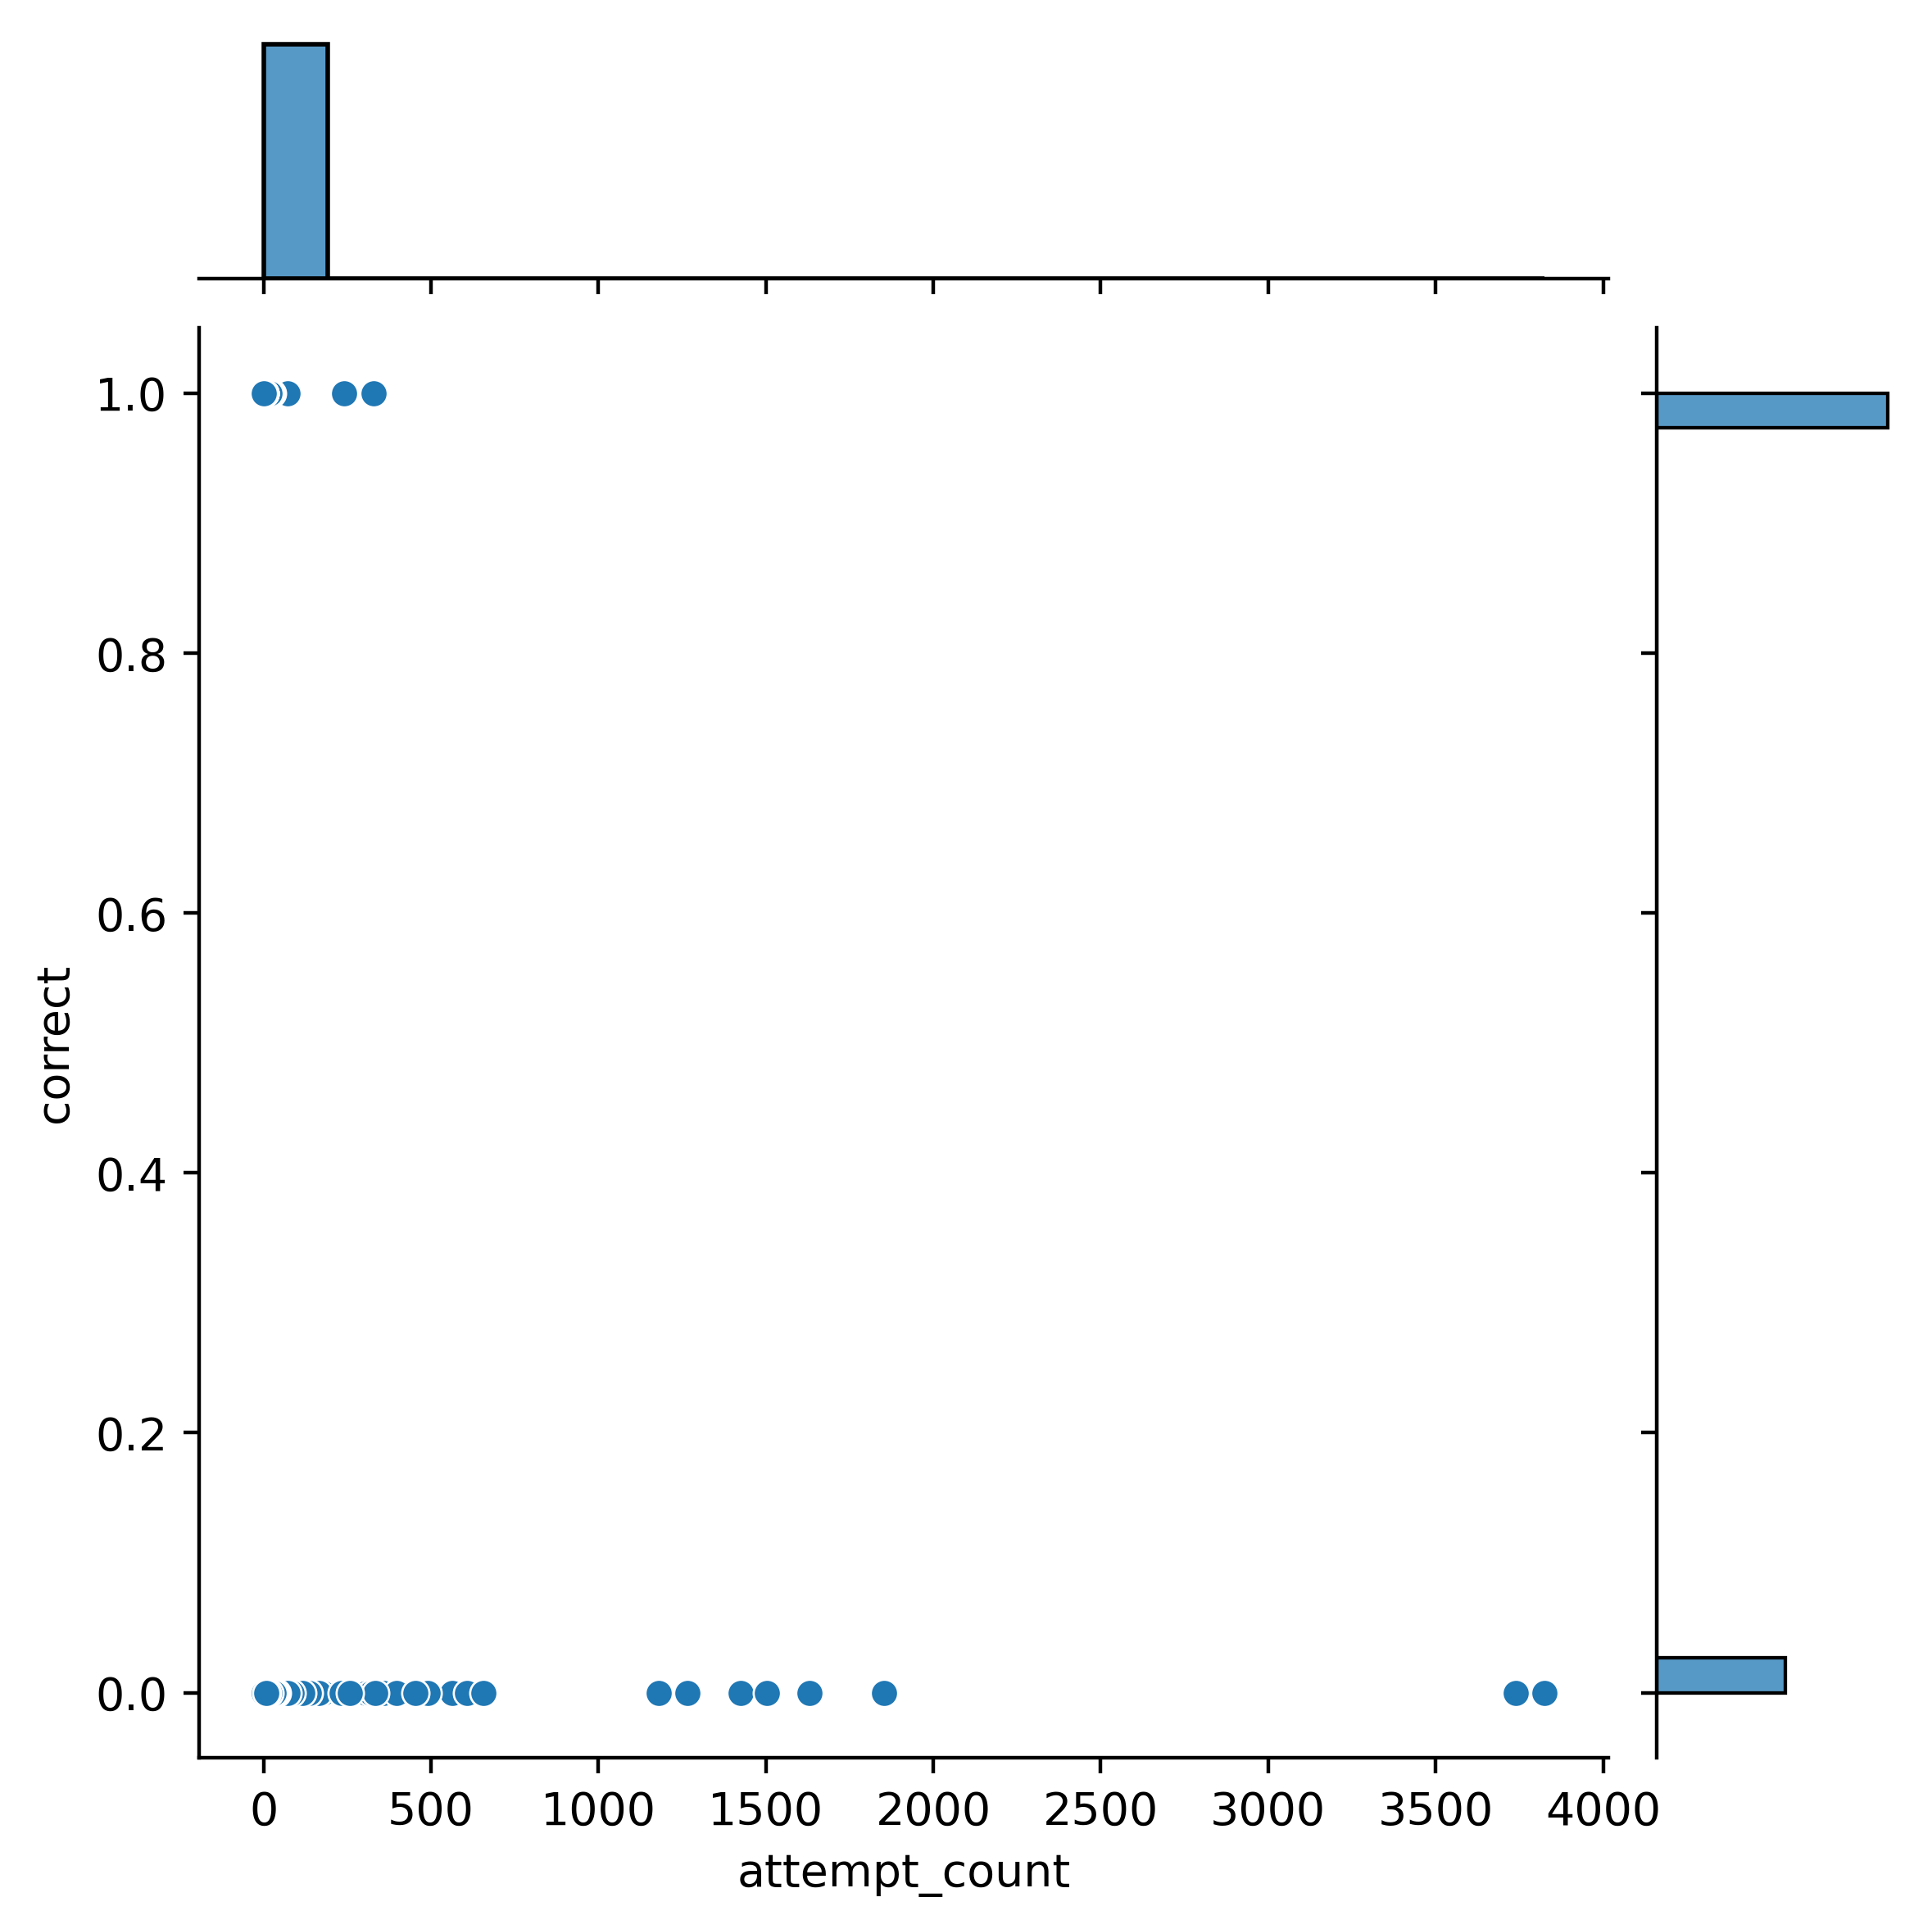
\includegraphics[width=0.85\textwidth]{ch3-jointplot-atc.png}
    \caption{The joint plot of attempt\_count}\label{fig:ch3-jointplot-atc}
\end{figure}

% \begin{figure}[htb]
%     \centering
%     \begin{subfigure}[b]{0.85\textwidth}
%         \centering
%         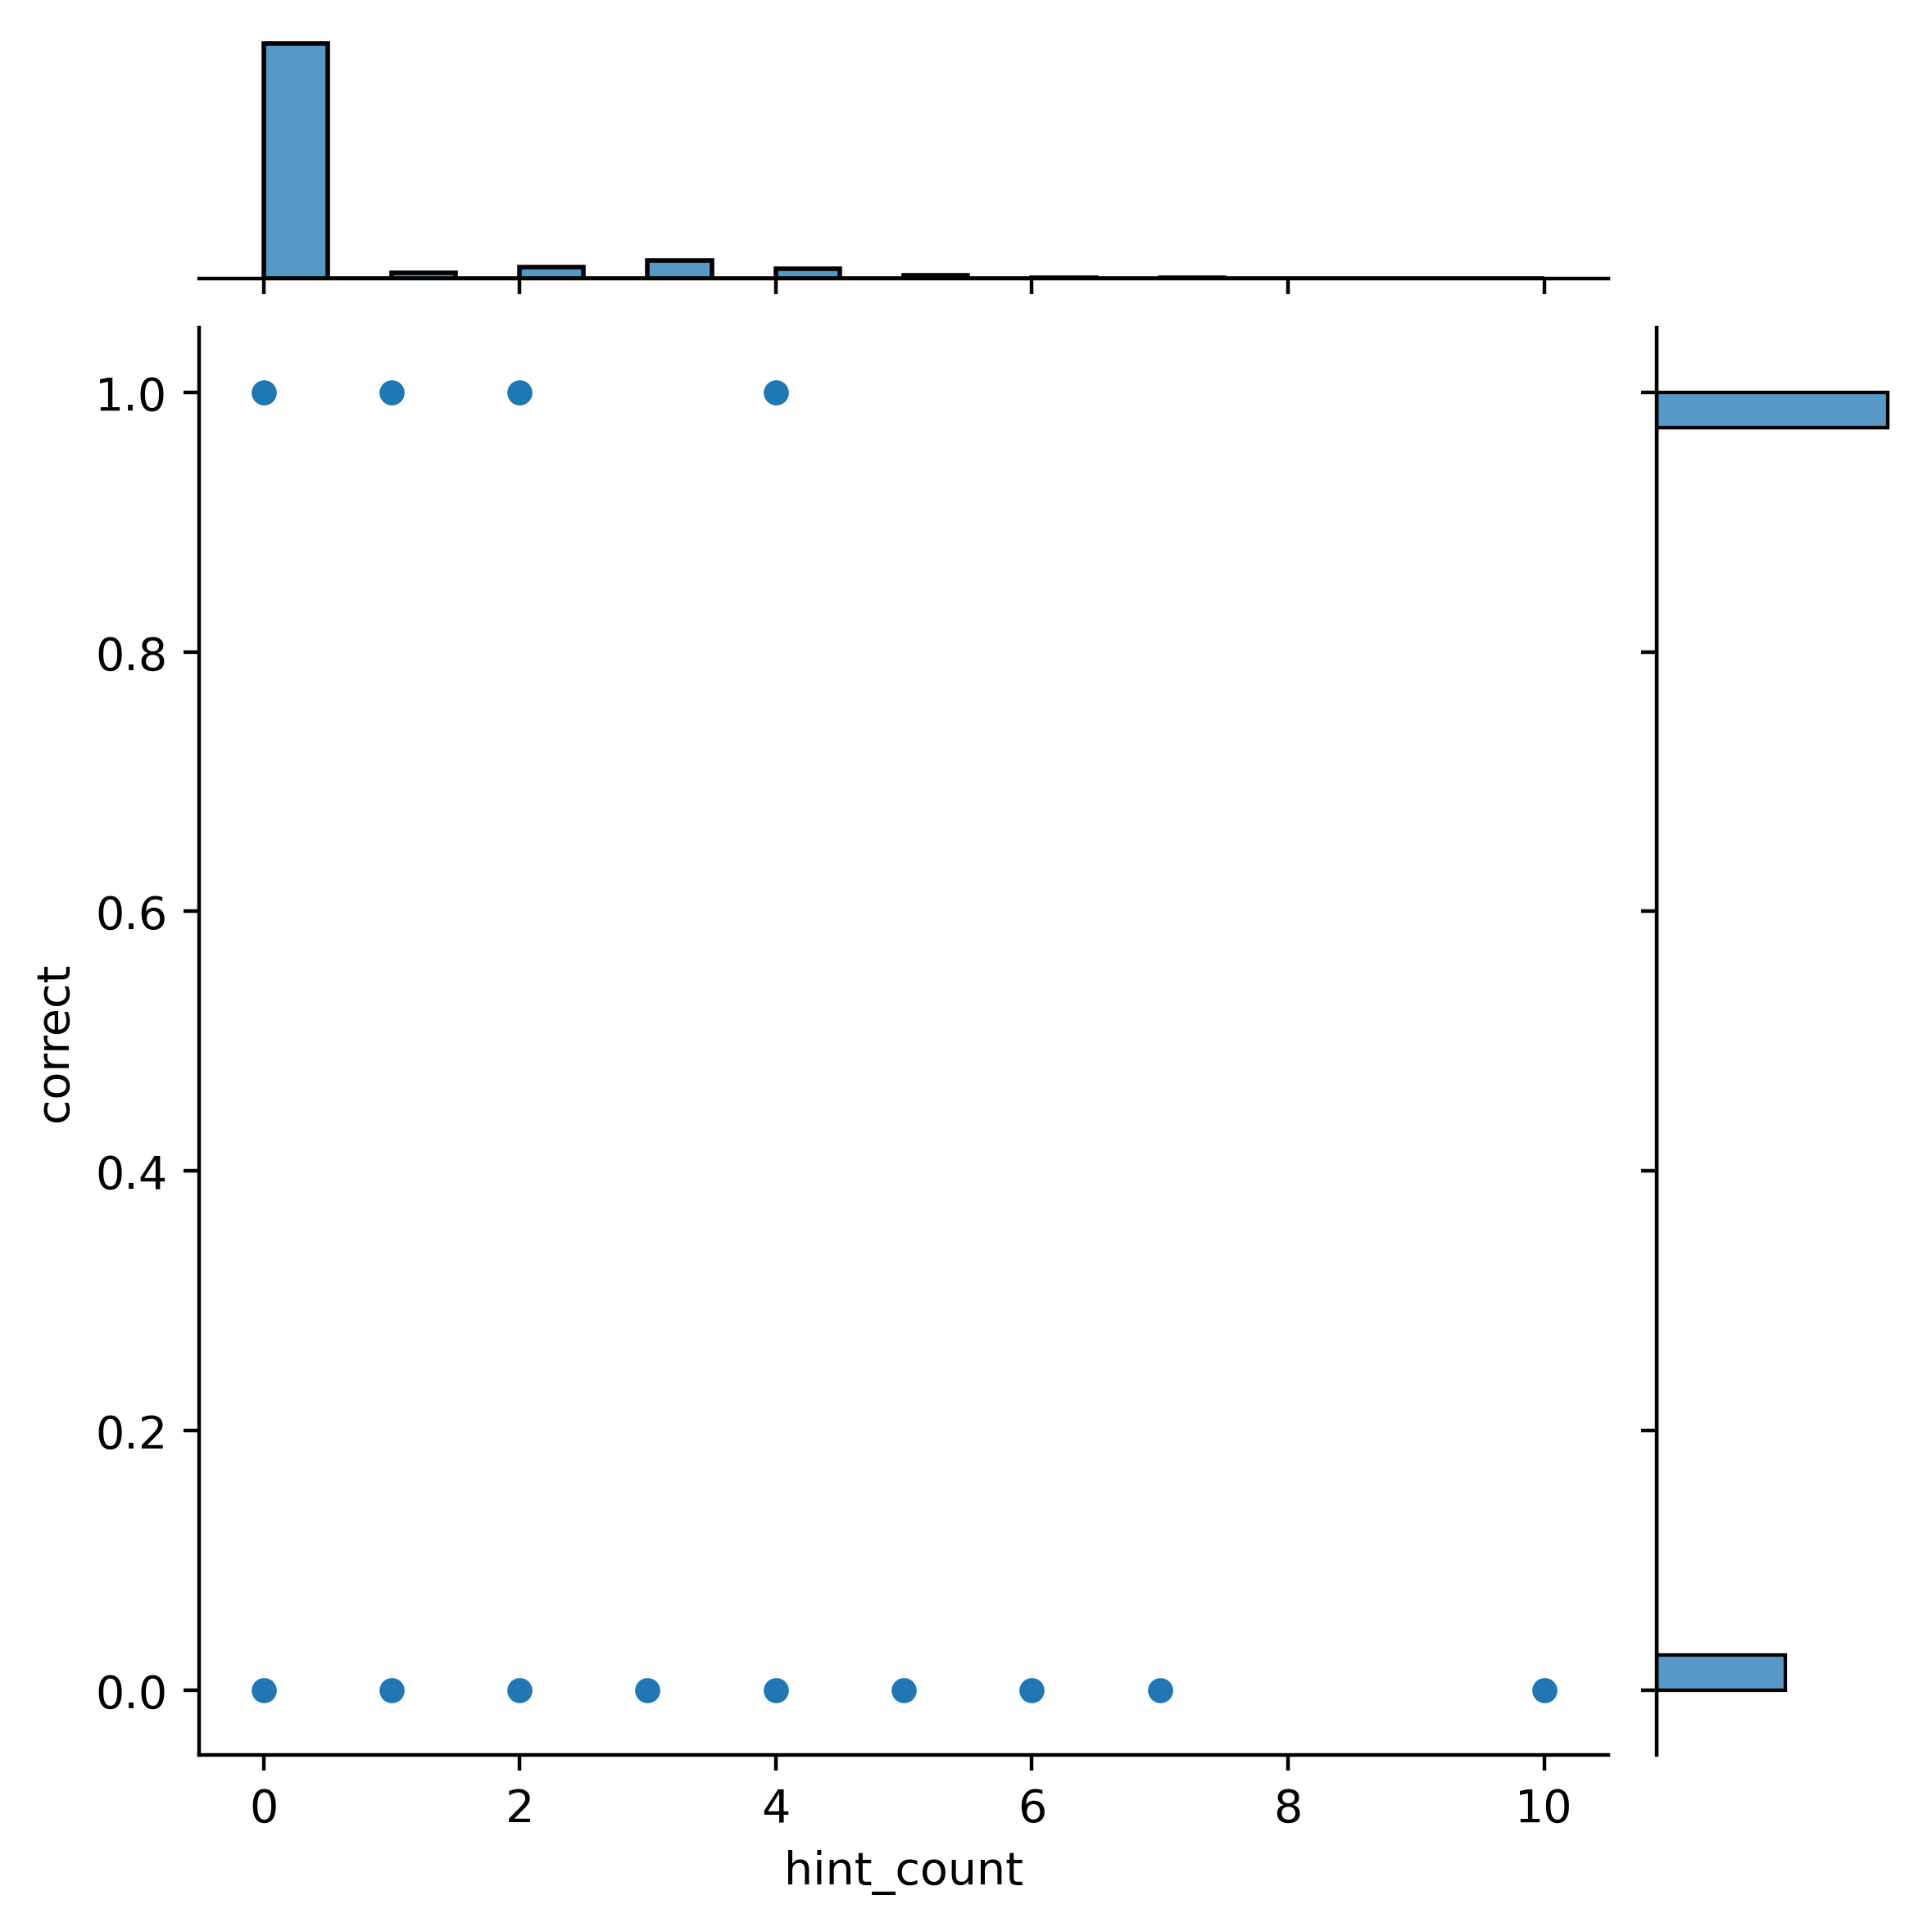
\includegraphics[width=0.9\textwidth]{ch3-jointplot-hc.png}
%         \caption{The joint-plot of hint\_count}\label{fig:ch3-jointplot-hc}
%     \end{subfigure}
%     \\
%     \begin{subfigure}[b]{0.85\textwidth}
%         \centering
%         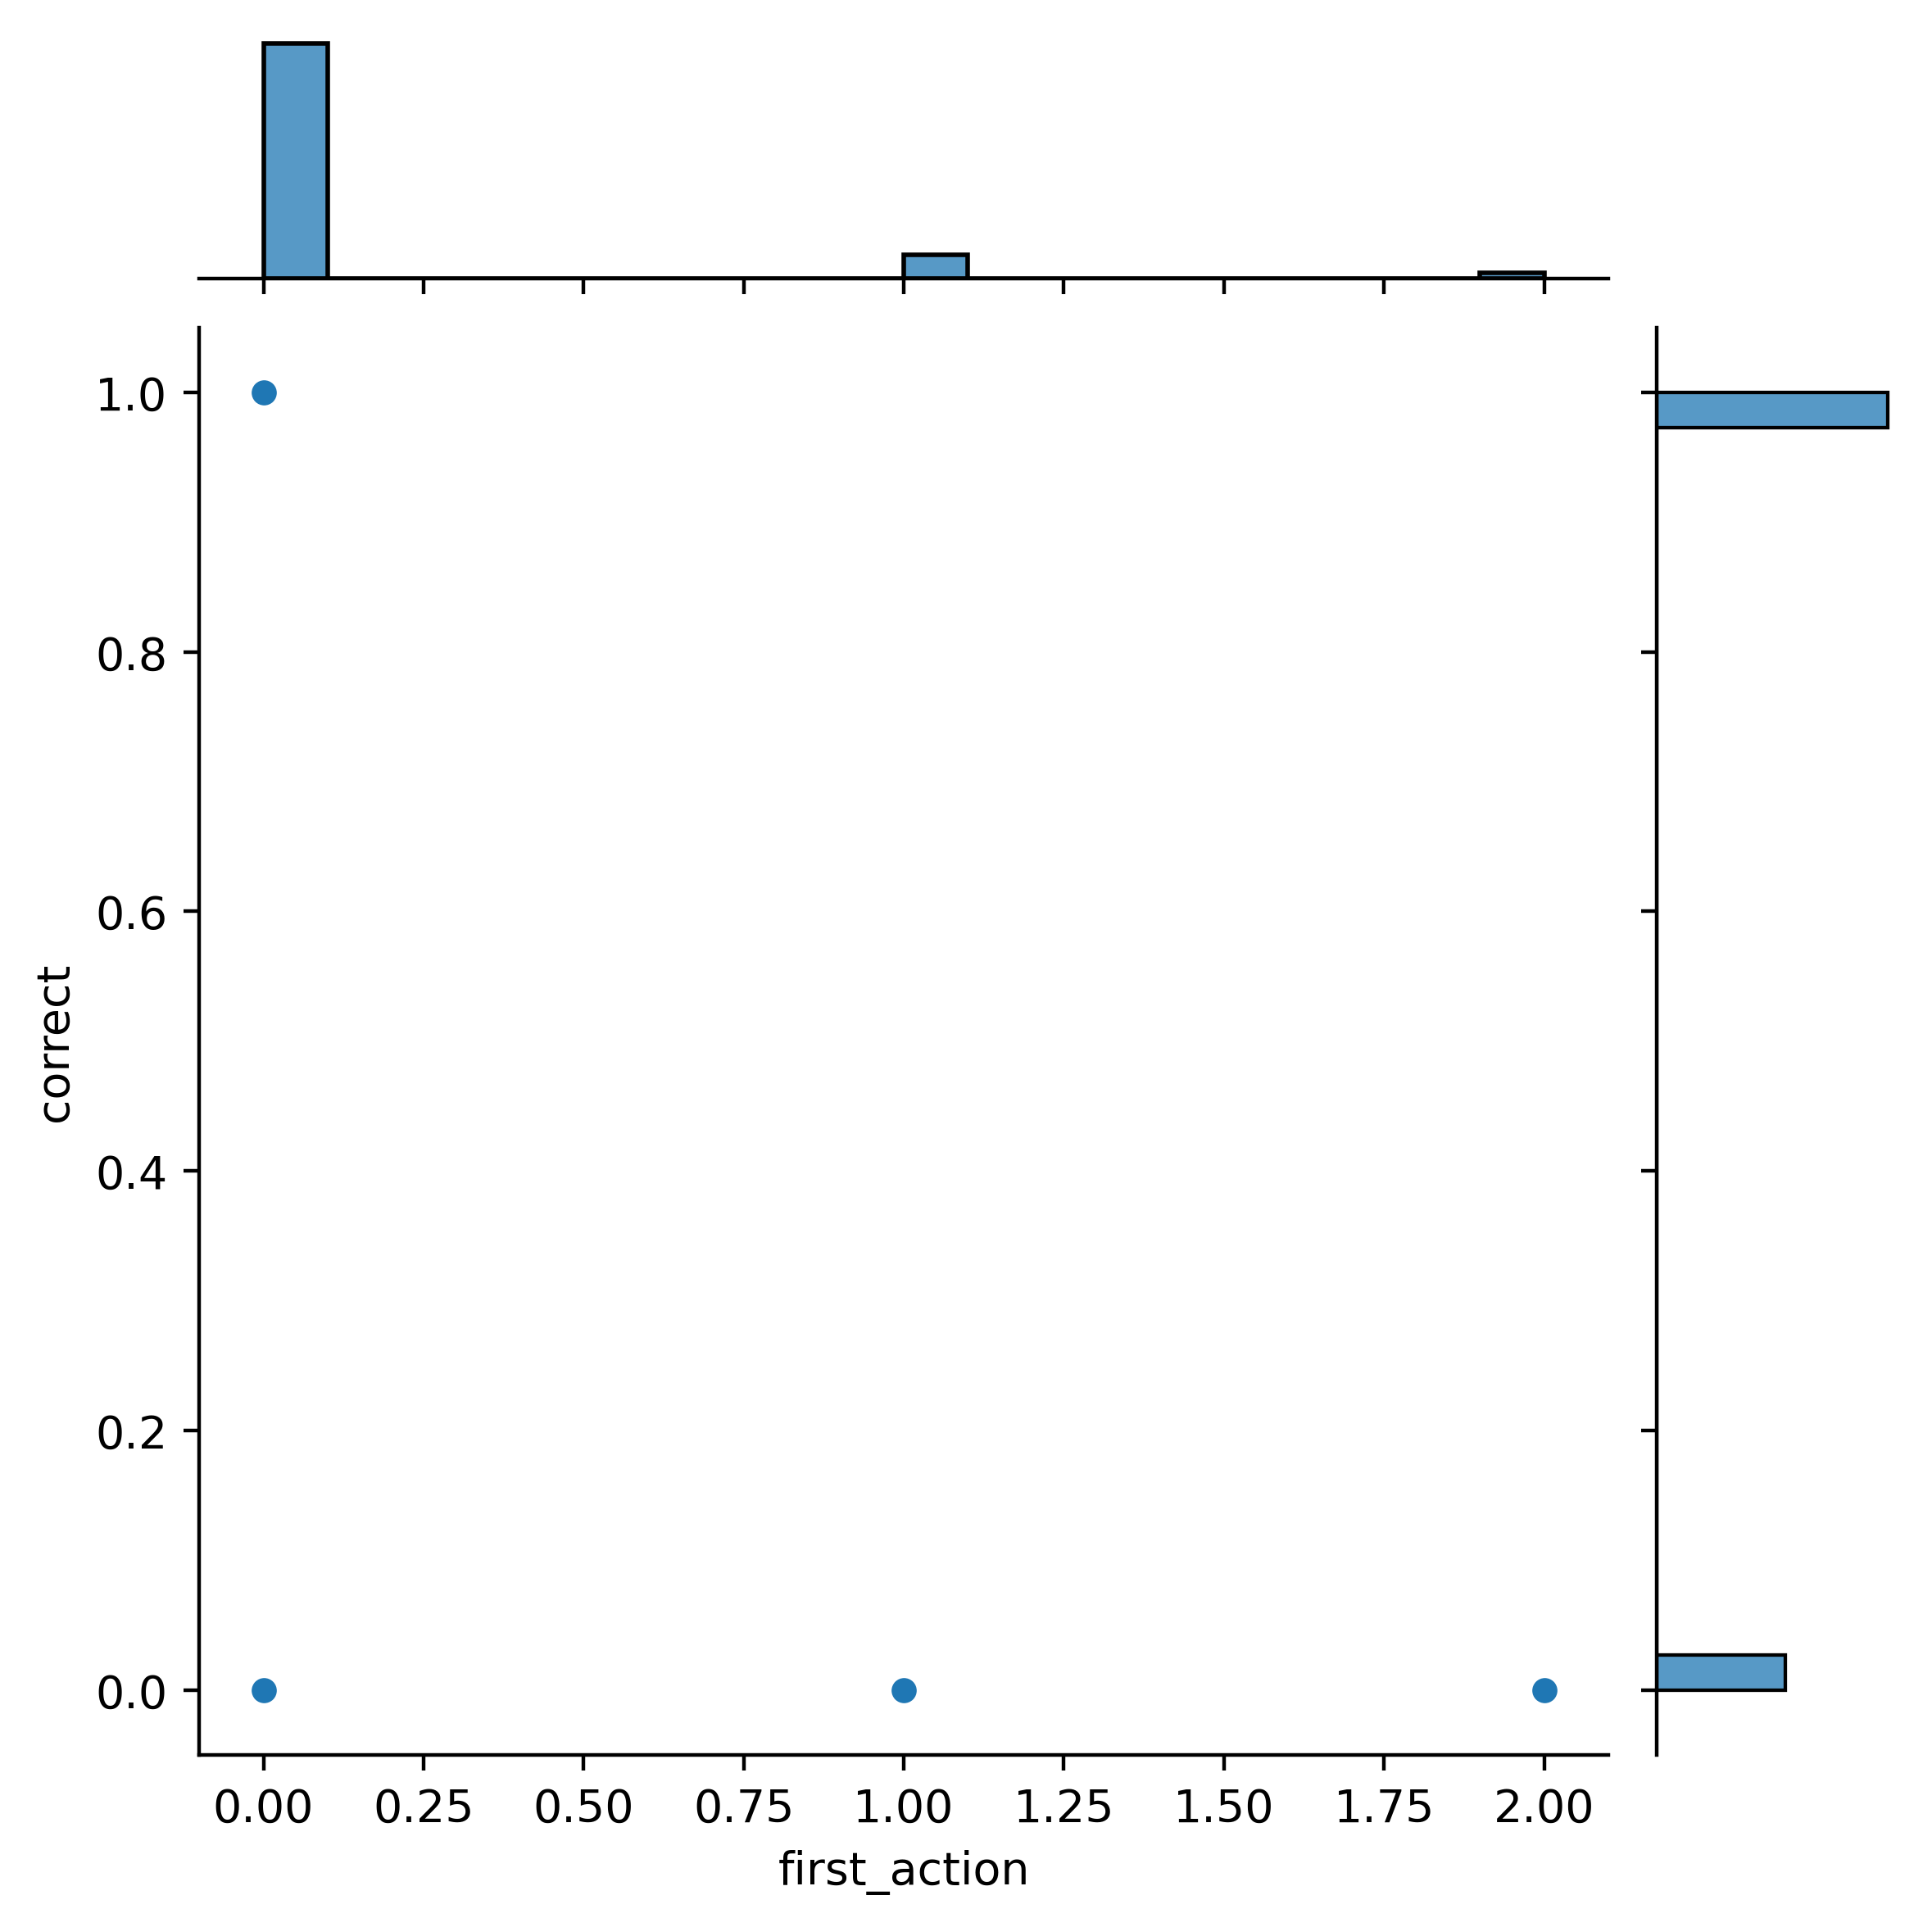
\includegraphics[width=0.9\textwidth]{ch3-jointplot-fc.png}
%         \caption{The joint-plot of first\_action}\label{fig:ch3-jointplot-fc}
%     \end{subfigure}
%     \\
%     \begin{subfigure}[b]{0.85\textwidth}
%         \centering
%         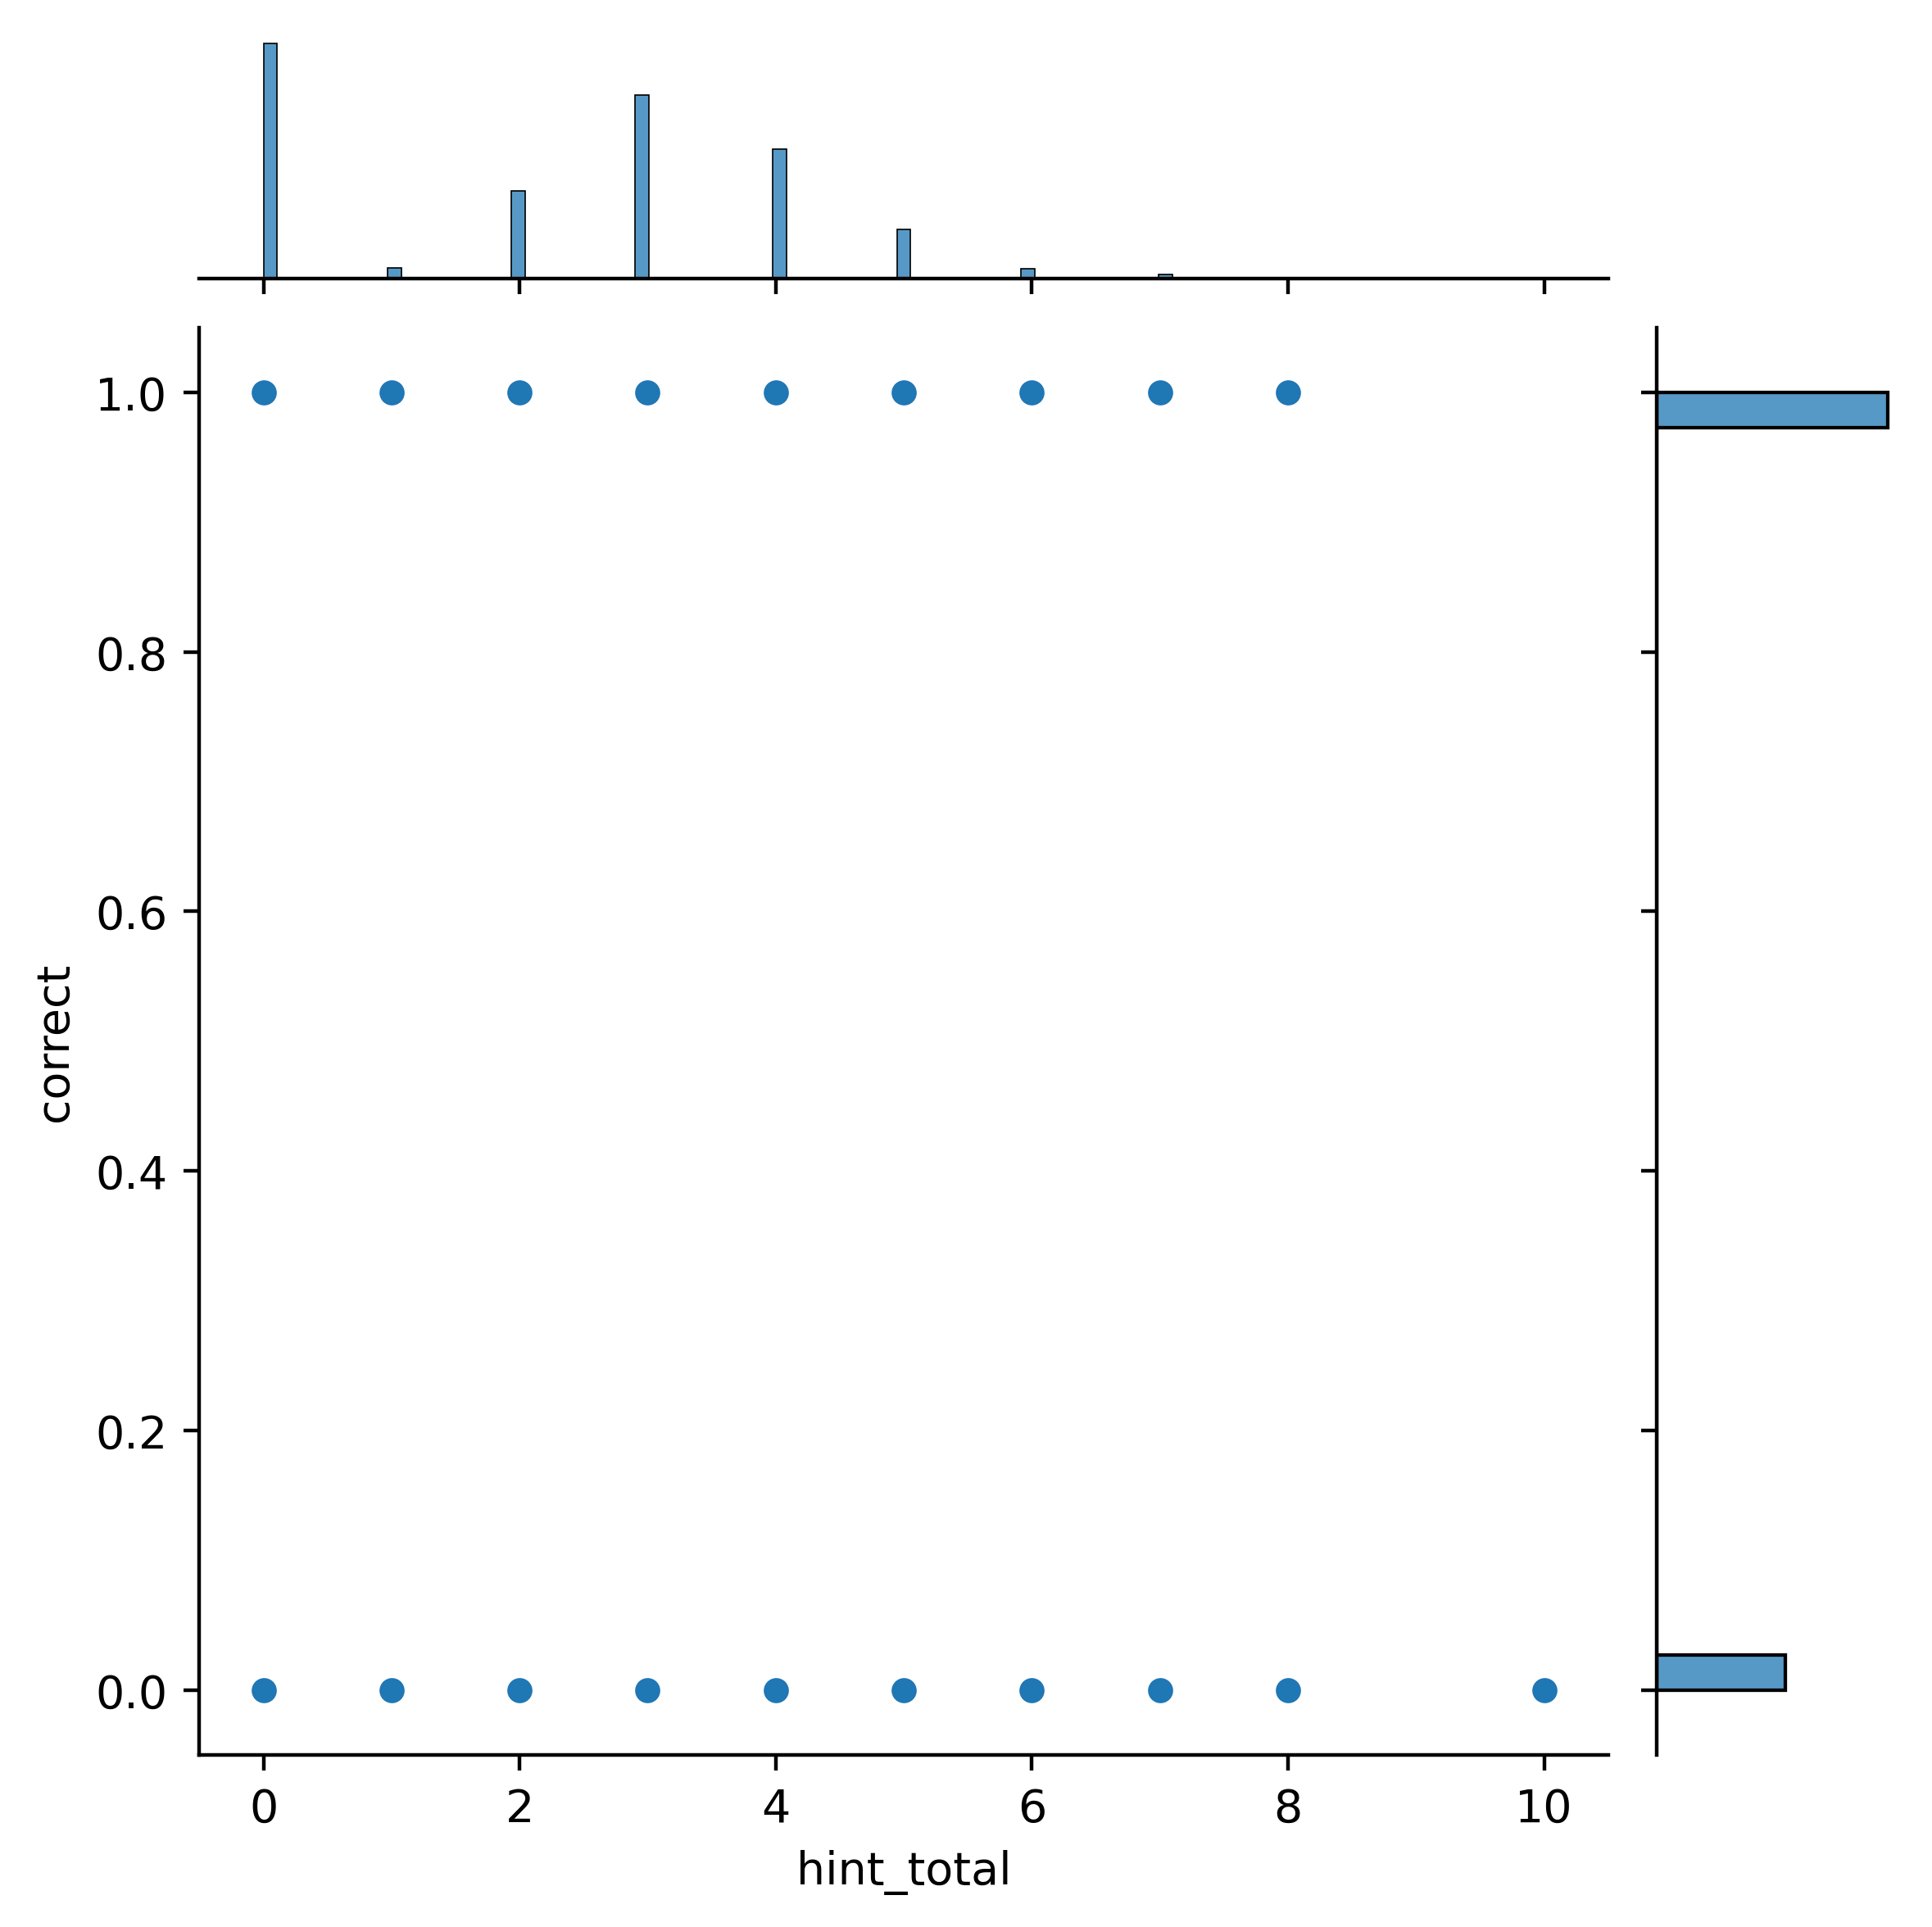
\includegraphics[width=0.9\textwidth]{ch3-jointplot-htc.png}
%         \caption{The joint-plot of hint\_total}\label{fig:ch3-jointplot-htc}
%     \end{subfigure}
%     \\
%     \begin{subfigure}[b]{0.85\textwidth}
%         \centering
%         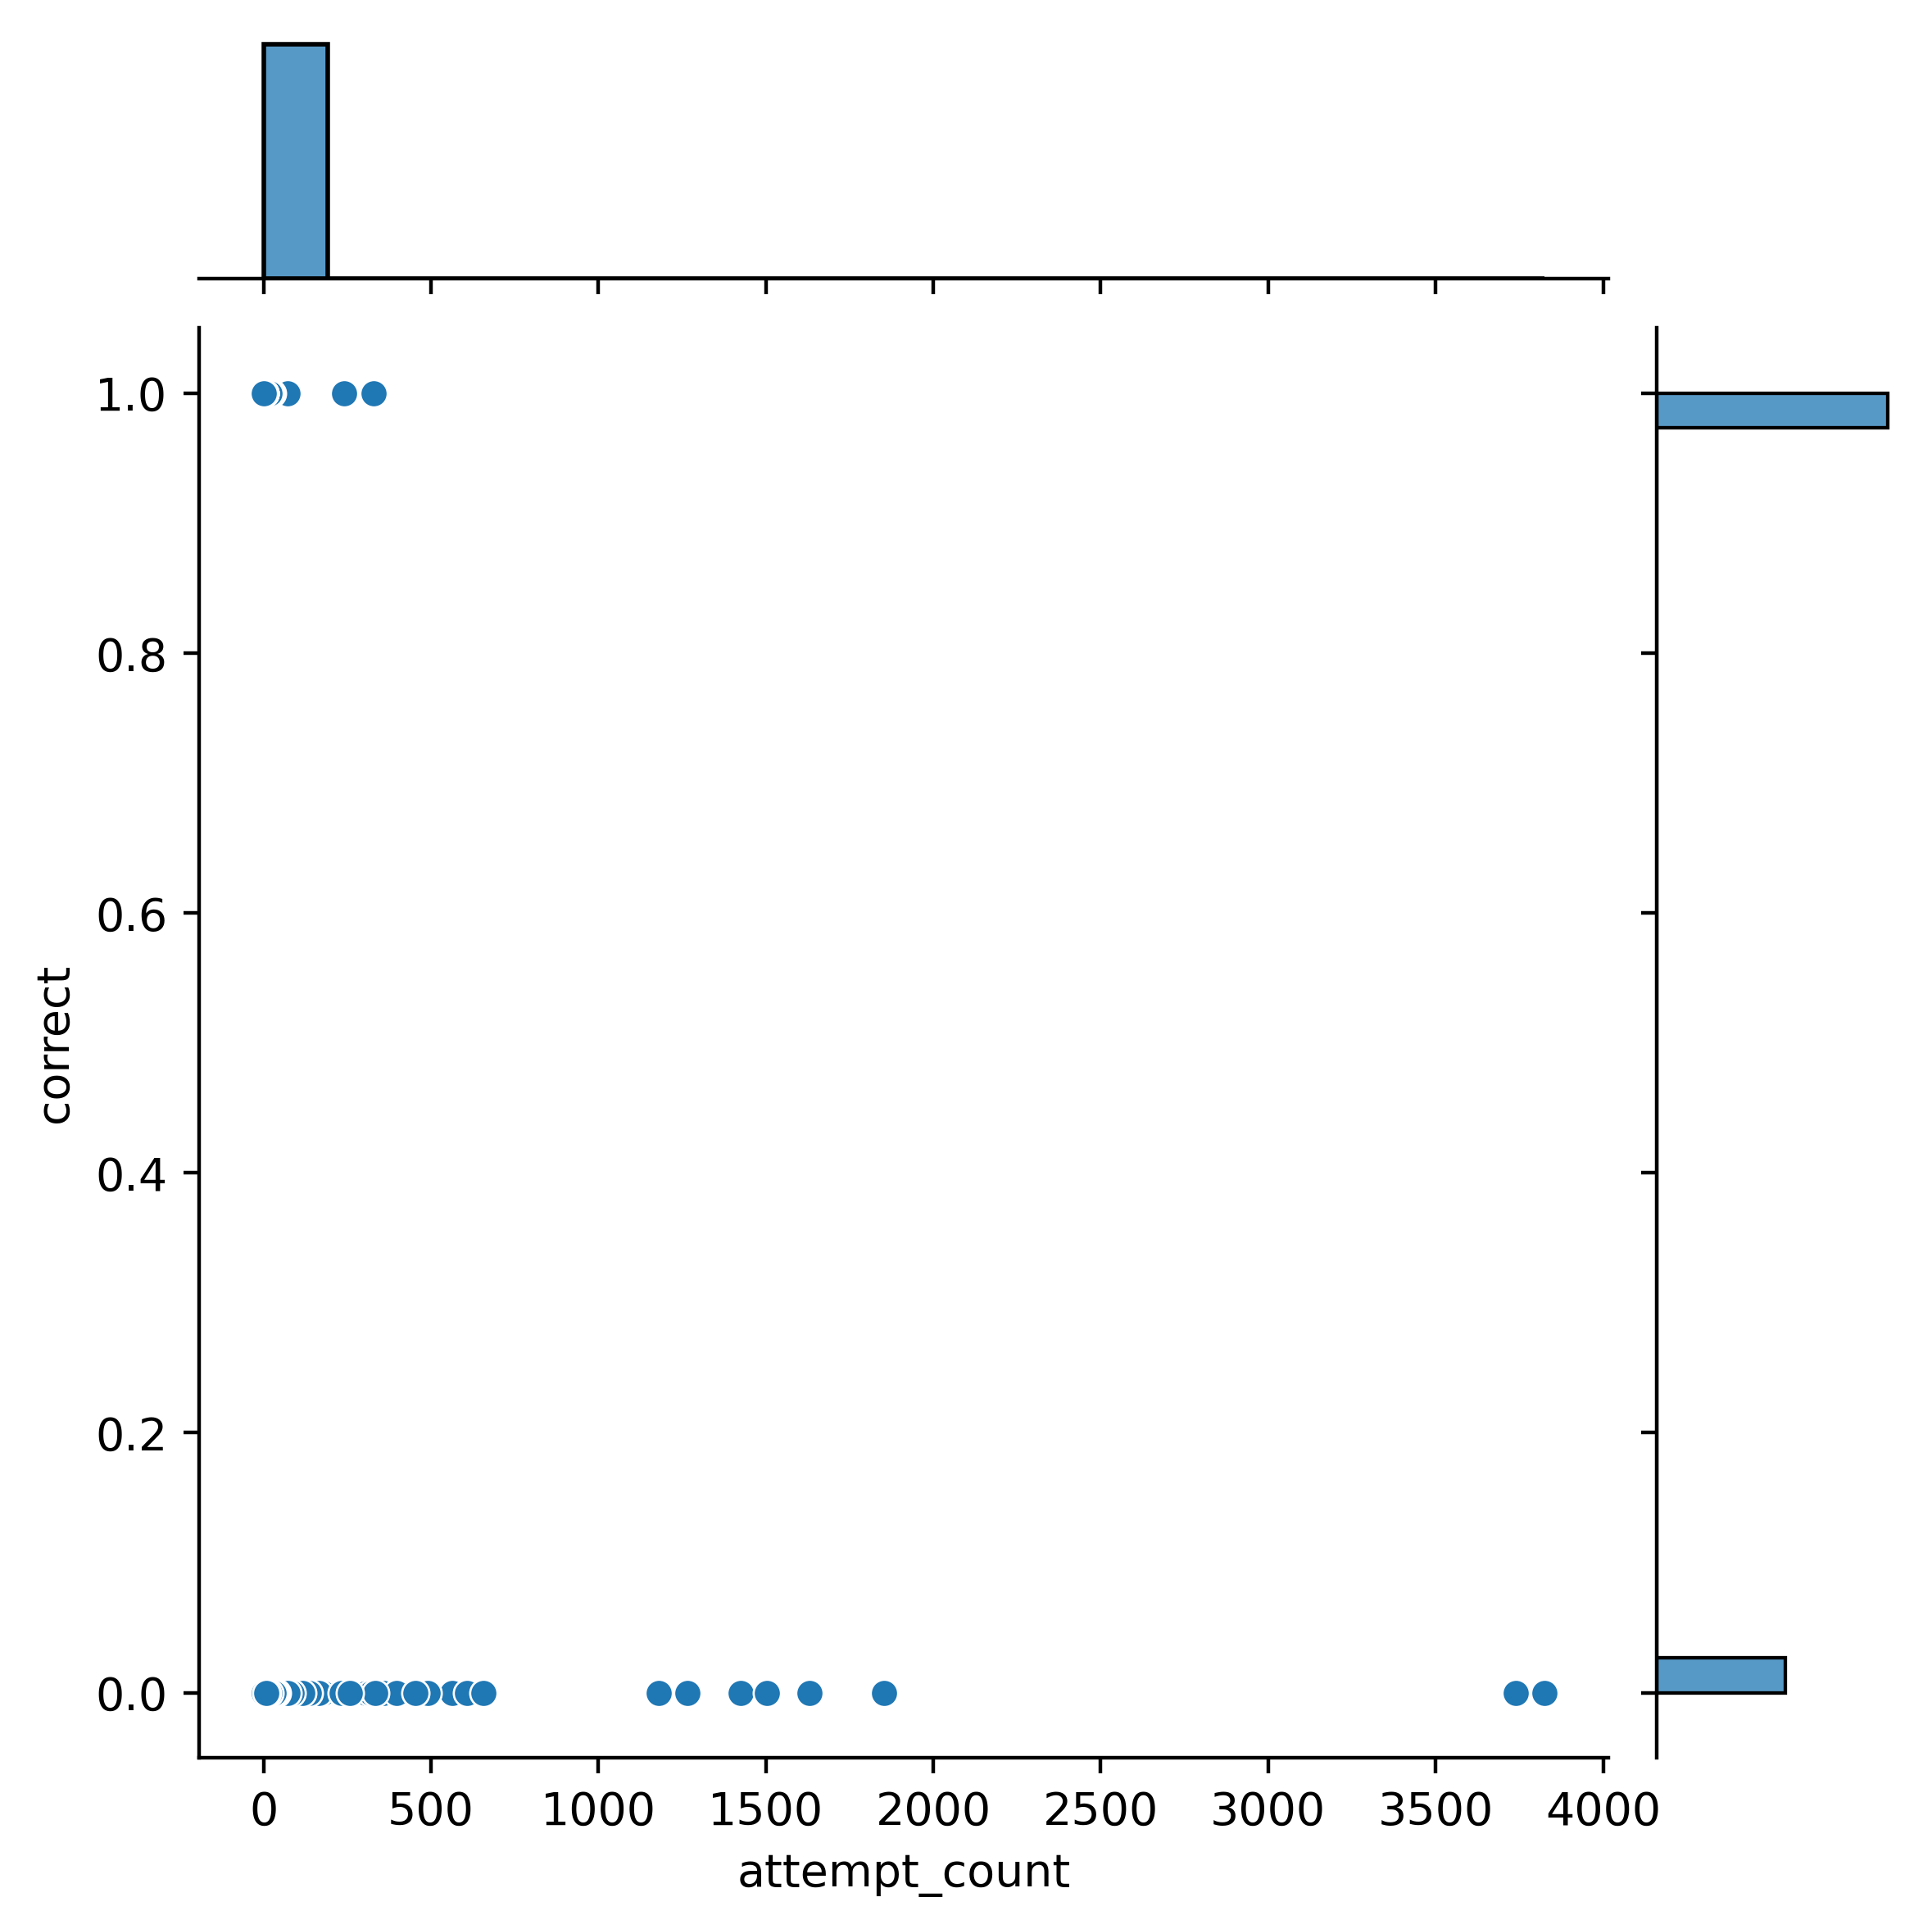
\includegraphics[width=0.9\textwidth]{ch3-jointplot-atc.png}
%         \caption{The joint-plot of attempt\_count}\label{fig:ch3-jointplot-atc}
%     \end{subfigure}
%     \caption{The joint-plots between input features and target feature}\label{fig:ch3-jointplots}
% \end{figure}

%经过上述分析,可以将上述四个特征作为模型的额外输入特征,可以作为判断最终输出的重要依据。
After the above analysis, the above four features can be used as additional input features for the model, which can be used as an important basis for judging the final output.
\subsection{Metrics}
%知识追踪本质上是一个分类问题,在机器学习领域中,常用的分类指标有Accuracy,Precision,Recall,F1 Score,AUC等。在二分类问题中,有如图\figname{\ref{fig:ch3-conmat}}的混淆矩阵,则这些分类指标的公式可以写作
Knowledge tracing is essentially a classification problem, where the commonly used classification metrics are Accuracy, Precision, Recall, F1 Score, etc. In the binary classification problem, there is the confusion matrix as shown in \figname{\ref{fig:ch3-conmat}}.
\begin{figure}[htbp!]
    \centering
    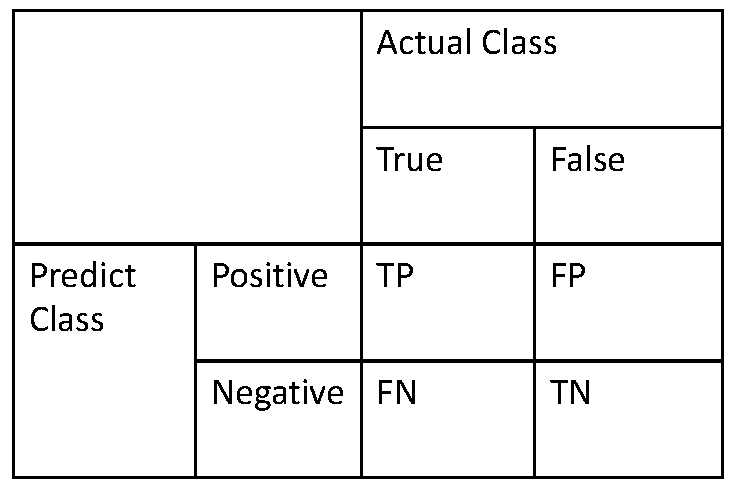
\includegraphics[width=0.85\textwidth]{ch3-conmat.pdf}
    \caption{The confusion matrix}\label{fig:ch3-conmat}
\end{figure}

Then, the formula for these classification indicators can be represented as \eqname{\ref{fml:ch3-conmat}}. The TP, TN, FP, FN represent true positive, true negative, false positive, and false negative. Although the Accuracy can determine the correct overall rate, the imbalance between positive and negative sample sizes can lead to high accuracy rates that do not fully measure the system's recognition performance for both categories. Additionally, Precision represents the proportion of true positive samples predicted as positive samples, which measures the accuracy of prediction of positive sample results, and Recall represents the bi l of true positive samples identified correctly. When Precision and Recall are plotted against each other, a P-R curve can be obtained. As Recall increases, Precision decreases overall, so a trade-off between the two is required. The F1 is a comprehensive indicator for weighing Precision and Recall.
\begin{align}\label{fml:ch3-conmat}
    \begin{split}
        \operatorname{Accuracy} &= \frac{TP+TN}{TP+TN+FP+FN} \\
        \operatorname{Precision} &= \frac{TP}{TP+FP} \\
        \operatorname{Recall} &= \frac{TP}{TP+FN} \\
        \operatorname{F1} &= \frac{2\times \operatorname{Precision}\times\operatorname{Recall}}{\operatorname{Precision}+\operatorname{Recall}}
    \end{split}
\end{align}
%为了解决样本不平衡的问题,即答对习题和答错习题量差别较大的情况,需要分别对正样本和负样本采用特定的统计特征。因此可以采取这种做法。其中\(\operatorname{TPR}=\operatorname{TP}/(\operatorname{TP}+\operatorname{FN})\)与\(\operatorname{FPR}=\operatorname{FP}/\operatorname{FP}+\operatorname{TN}\)基于实际的正样本和负样本进行统计,排除了样本不平衡的影响。FPR 表示模型虚报的响应程度,TRP表示出模型预测相应的覆盖程度。将FPR作为x轴,TPR作为y轴,则可以绘制出Receiver Operating Characteristic曲线,该曲线可以评价模型的预测能力。随着不断遍历所有的分类阈值,FPR和TPR会随着ROC曲线变动。根据上述统计量可以推知,当TPR 越高,同时 FPR 越低,ROC曲线越陡峭,那么模型的性能就越好。 它可以解决样本不平衡的问题。
To address the problem of sample imbalance, i.e., a large difference in the amount of correct and incorrect answers to an exercise, specific statistical characteristics need to be applied to the positive and negative samples, respectively. The \(\operatorname{TPR}=\operatorname{TP}/(\operatorname{TP}+\operatorname{FN})\) and \(\operatorname{FPR}=\operatorname{FP}/\operatorname{FP}+\operatorname{TN}\) based on the actual positive and negative samples can be applied for the statistics, excluding the effect of sample imbalance. \(\operatorname{FPR}\) indicates the degree of response that the model falsely reports, and \(\operatorname{TPR}\) indicates the corresponding degree of coverage predicted by the model. Taking FPR as the x-axis and TPR as the y-axis, a Receiver Operating Characteristic (ROC) curve can be plotted, which evaluates the model's predictive ability. As all the classification thresholds are traversed, the FPR and TPR will change with the ROC curve. The ROC curve is also plotted by traversing all the classification thresholds, which can solve the problem of sample imbalance. Based on the above analysis, it can be inferred that when the TPR is higher and at the same time the FPR is lower, the steeper the ROC curve is, then the performance of the model is better. It can solve the problem of sample imbalance.


%目前知识追踪领域的论文多以(Area Under Curve)AUC作为对比指标,AUC是一个基于ROC曲线常用的二分类评测手段,具有较好的性能对比能力。在知识追踪任务中,最终预测也是当前时刻的习题的做对与否,本质上为一个二分类问题,
To measure the ROC curve's steepness, Area Under Curve (AUC) can be a suitable statistic. AUC is a commonly used two-category evaluation method based on the ROC curve and has good performance comparison capabilities. The closer the AUC is to 1, the stronger the predictive performance of the model. At present, most papers in the field of knowledge tracing use AUC as a comparison indicator. In the task of knowledge tracing, the final prediction is whether the exercises at the current moment are done correctly or not, which is essentially a binary classification problem so that this approach can be adopted.

\subsection{Experiment Settings}
%本实验采用KFold方法分割测试集和验证集,取\(K=5\)。原始数据经过处理,会将每个学生的做题序列进行隔离,超过预定最长序列长度的学生会被分割成若干个不超过最长长度的序列。而实验可以采用不同的知识追踪对象进行交叉验证实验,可以有效衡量模型的预测性能。
This experiment uses the KFold method to partition the test and validation sets, taking \(K=5\). The raw data are processed to segregate the sequence of questions done by each student, and students who exceed the predetermined longest sequence length are split into several sequences that do not exceed the longest length. Moreover, the experiments can use different knowledge tracing objects for cross-validation experiments, which can effectively measure the model's prediction performance.
%本实验主要运行在深度学习服务器上,运行环境见表.

This experiment runs on a dedicated GPU computing server, and the running environment is shown in \tblname{\ref{tbl:ch3-exp-env}}.
\begin{table}[htbp!]
    \caption{Experiment running environment}\label{tbl:ch3-exp-env}
    \centering
    \begin{tabular}{l c}
        \toprule
        Software/Hardware & Configuration   \\
        \midrule
        CPU               & Xeon Gold 6139  \\
        GPU               & Tesla V100      \\
        VRAM              & 16G             \\
        Operating System  & Ubuntu 18.04    \\
        Python            & 3.8.6           \\
        PyTorch           & 1.8.0           \\
        GPU Driver        & Cuda11.2/cudnn8 \\
        \bottomrule
    \end{tabular}
\end{table}


\subsection{Baselines}
%1.BKT是一个知识追踪的经典模型,它基于隐马尔可夫模型(HMM),将学习者的知识状态建模为一组对应知识点掌握情况的二元变量。
%2.DKT是第一个基于深度学习的知识追踪模型,它应用将学生的做题记录输入到LSTM中,可以捕获学生做题序列上近期做题记录的影响,将学生的做题顺序考虑进模型,DKT也初步考虑了知识点间的内在相关性。
%3.GKT应用图神经网络到知识追踪任务上,利用图的特性,将知识点间的图状关联表征出来,从而更好地学习知识内在依赖关系,该模型能够学习出学生的隐藏知识状态,也具有较好的可解释性。
In this experiment, baseline performance comparisons are made by comparing some classic models with new knowledge tracing models proposed recently. The following models are evaluated in performance comparison.
\begin{itemize}
    \item Deep knowledge tracing~\cite{piech2015deep}: DKT applies the input of students' doing records into LSTM and can capture the influence of recent doing records on students' doing sequences, taking students' doing sequences into account into the model; DKT also initially considers the intrinsic correlation between knowledge points.
    \item Dynamic key-value memory networks (DKVMN)~\cite{zhang2017dynamic}: DKVMN uses key-value pairs as the memory structure, which can avoid over better prediction performance relative to BKT, and DKT is achieved by using key-value pairs as the memory structure.
    \item Self-attentive model for knowledge tracing (SAKT)~\cite{sakt2019}: The SAKT model takes into account the correlation between exercises in terms of potential knowledge points and introduces the Transformer structure to calculate the Attention between input sequences of exercises so that the relevance of current exercises can be calculated based on previous exercises and reasonable predictions can be made.
    \item Neural pedagogical agent (NPA)~\cite{Lee2019CreatingAN}: NPA applied Attention-based Bi-LSTM model to the knowledge tracing task, which takes into account the bidirectional information of the question-answering sequence, and the subsequent answer sequence interactions also correct the previous predictions.
\end{itemize}

\subsection{Model Training}
%本模型需要预定义一些训练参数,经过参数调整,得到如表\figname{\ref{tbl:ch3-hpsetting}}所示的参数组合
This model requires some predefined training parameters, and after parameter adjustment, the parameter combinations shown in \tblname{\ref{tbl:ch3-hpsetting}} are obtained.
\begin{table}[htbp!]
    \caption{Hyperparameter settings of proposed model}\label{tbl:ch3-hpsetting}
    \centering
    \begin{tabular}{l l c}
        \toprule
        Hyperparameter & Description                             & Value \\
        \midrule
        lr             & learning rate                           & 0.01  \\
        opt            & optimizer                               & Adam  \\
        batch\_size    & batch size                              & 32    \\
        maxseqlen      & maximum sequence length                 & 200   \\
        q\_embed\_dim  & exercise embedding dimension            & 50    \\
        qa\_embed\_dim & exercise  answering embedding dimension & 20    \\
        memory\_size   & number of memory slots                  & 20    \\
        \bottomrule
    \end{tabular}
\end{table}
%实验总共进行了三次训练,选取了平均的训练过程参数进行训练数据图绘制,得到损失训练图和模型性能训练图,如图所示。可见在150轮时,模型基本上收敛。
The experiments were conducted a total of three times, and the average training output was selected for training data plotting to obtain the loss training plot and the model performance training plot, as shown in \figname{\ref{fig:ch3-train-loss}} and \figname{\ref{fig:ch3-train-acc}}. It can be seen that the model basically converges after about 150 epochs.
\begin{figure}[htb]
    \centering
    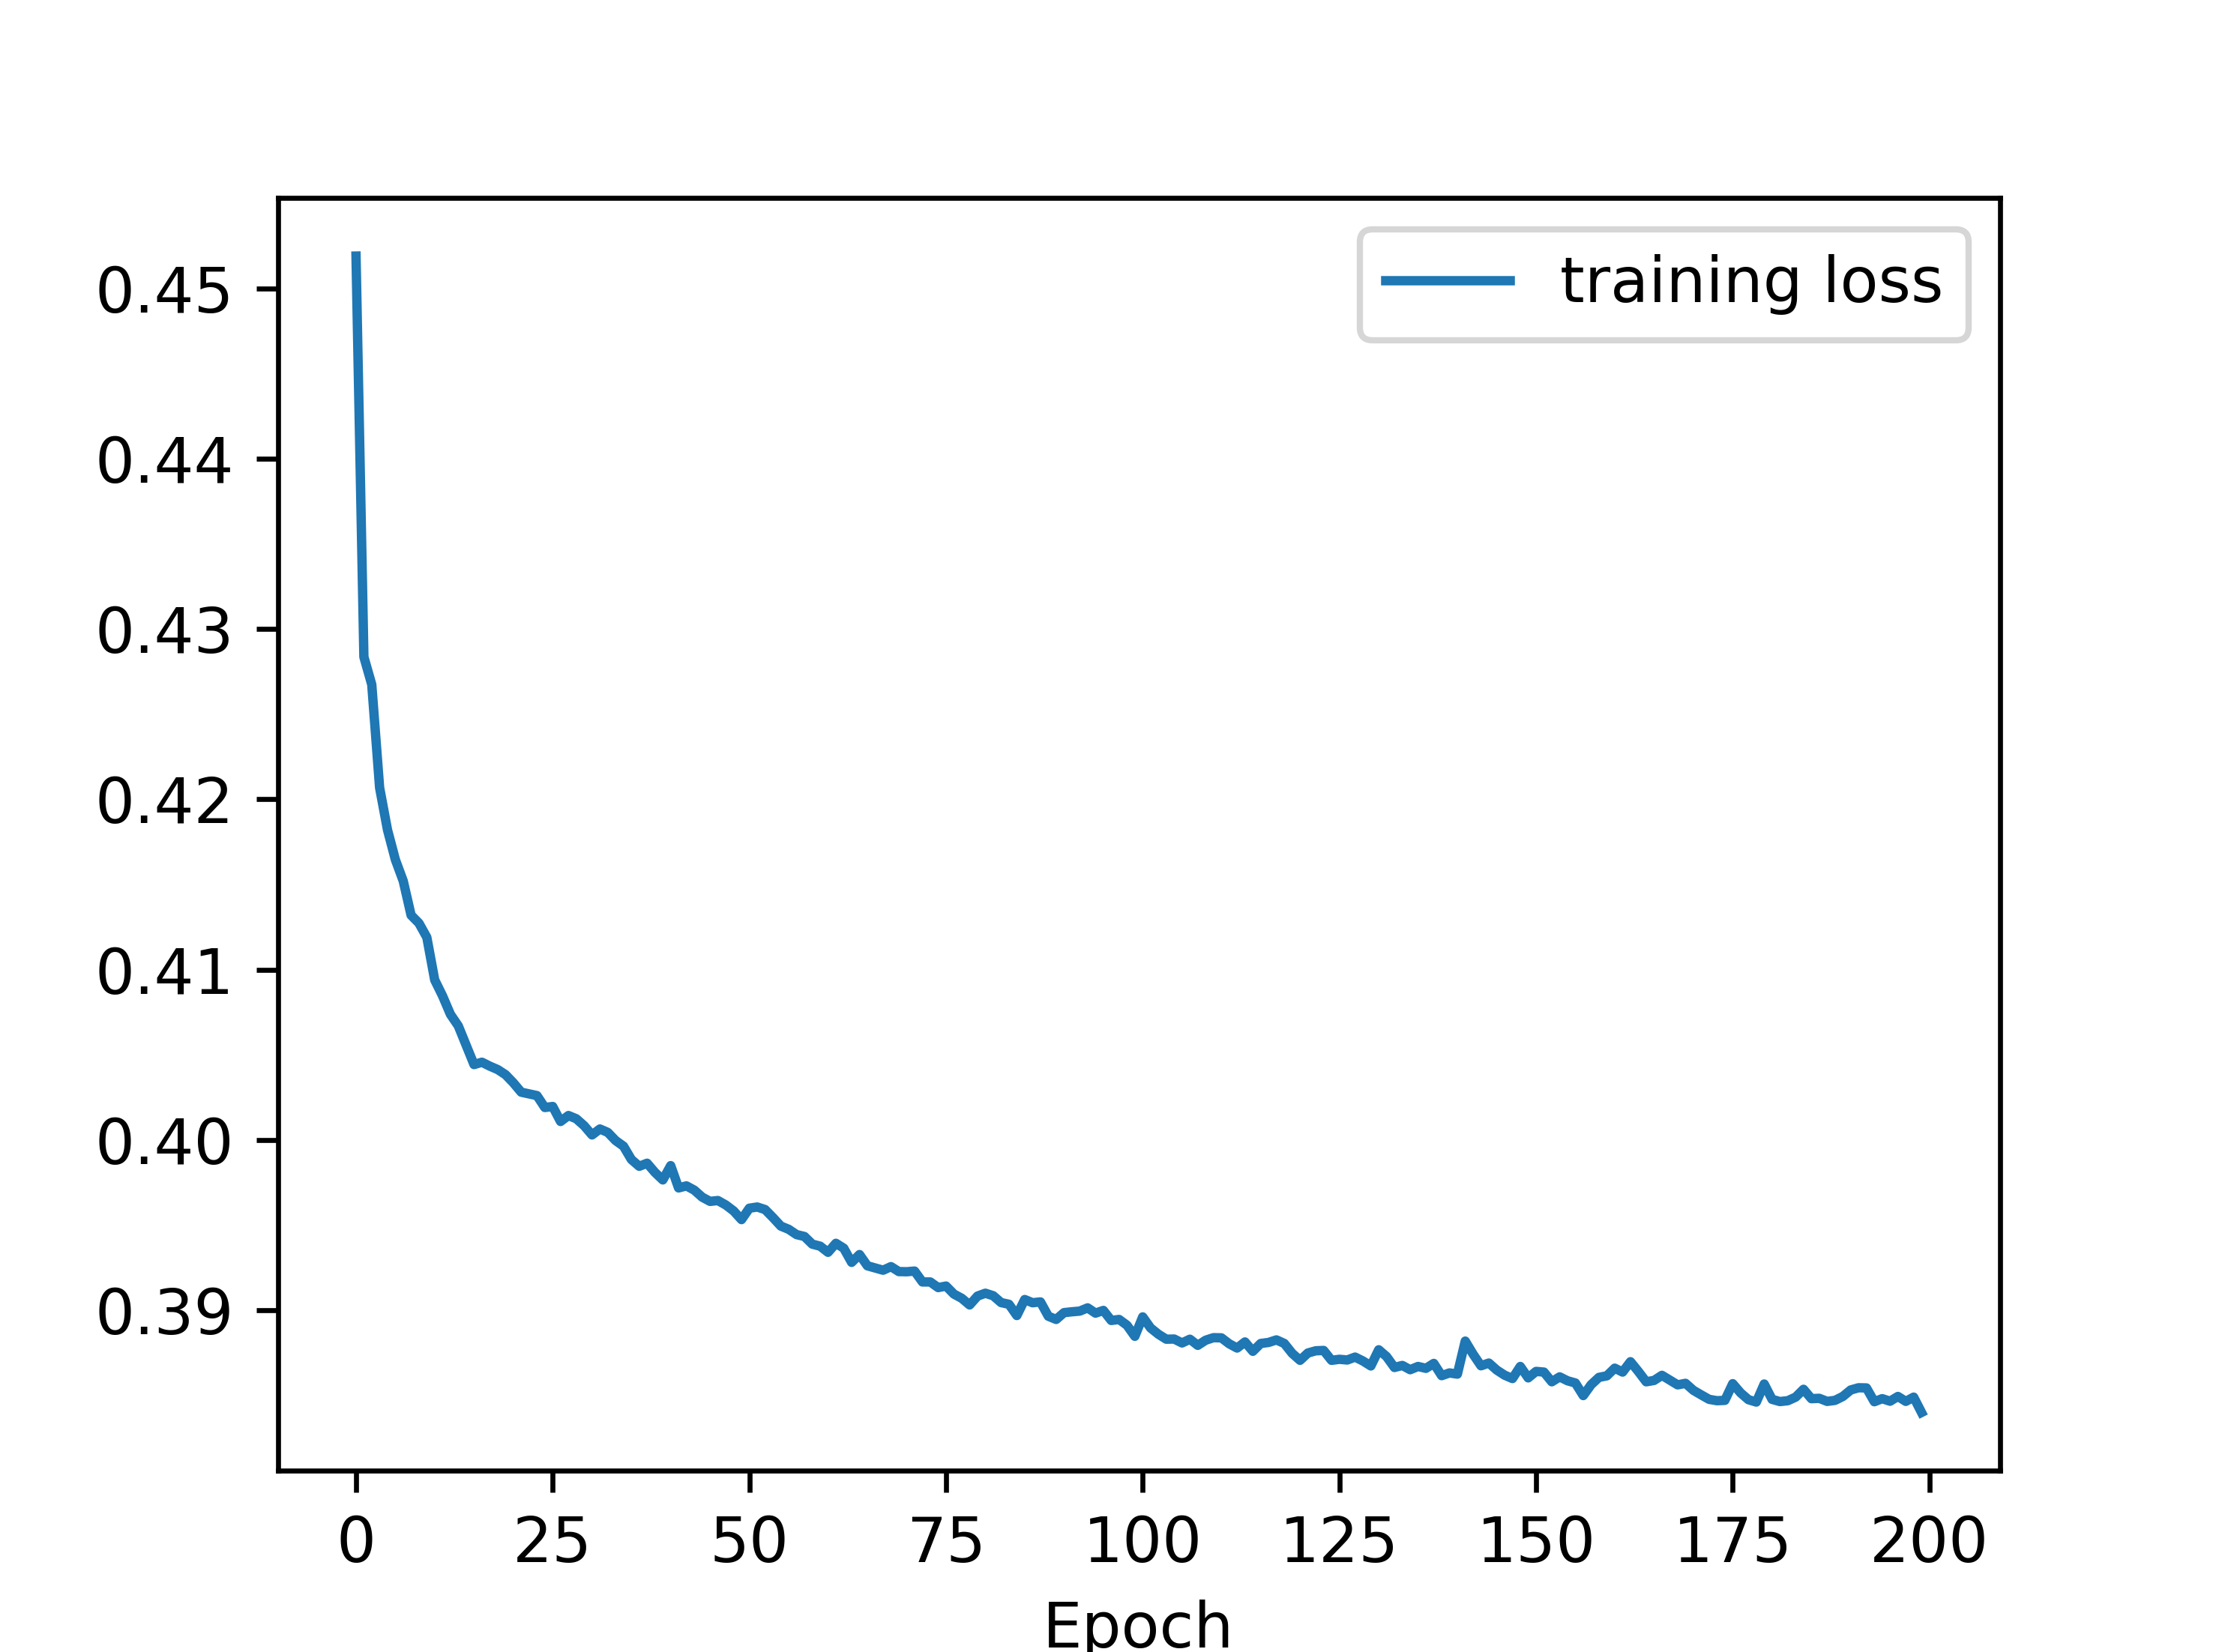
\includegraphics[width=0.9\textwidth]{ch3-train-loss.png}
    \caption{The training process of proposed model}\label{fig:ch3-train-loss}
\end{figure}

\begin{figure}[htb]
    \centering
    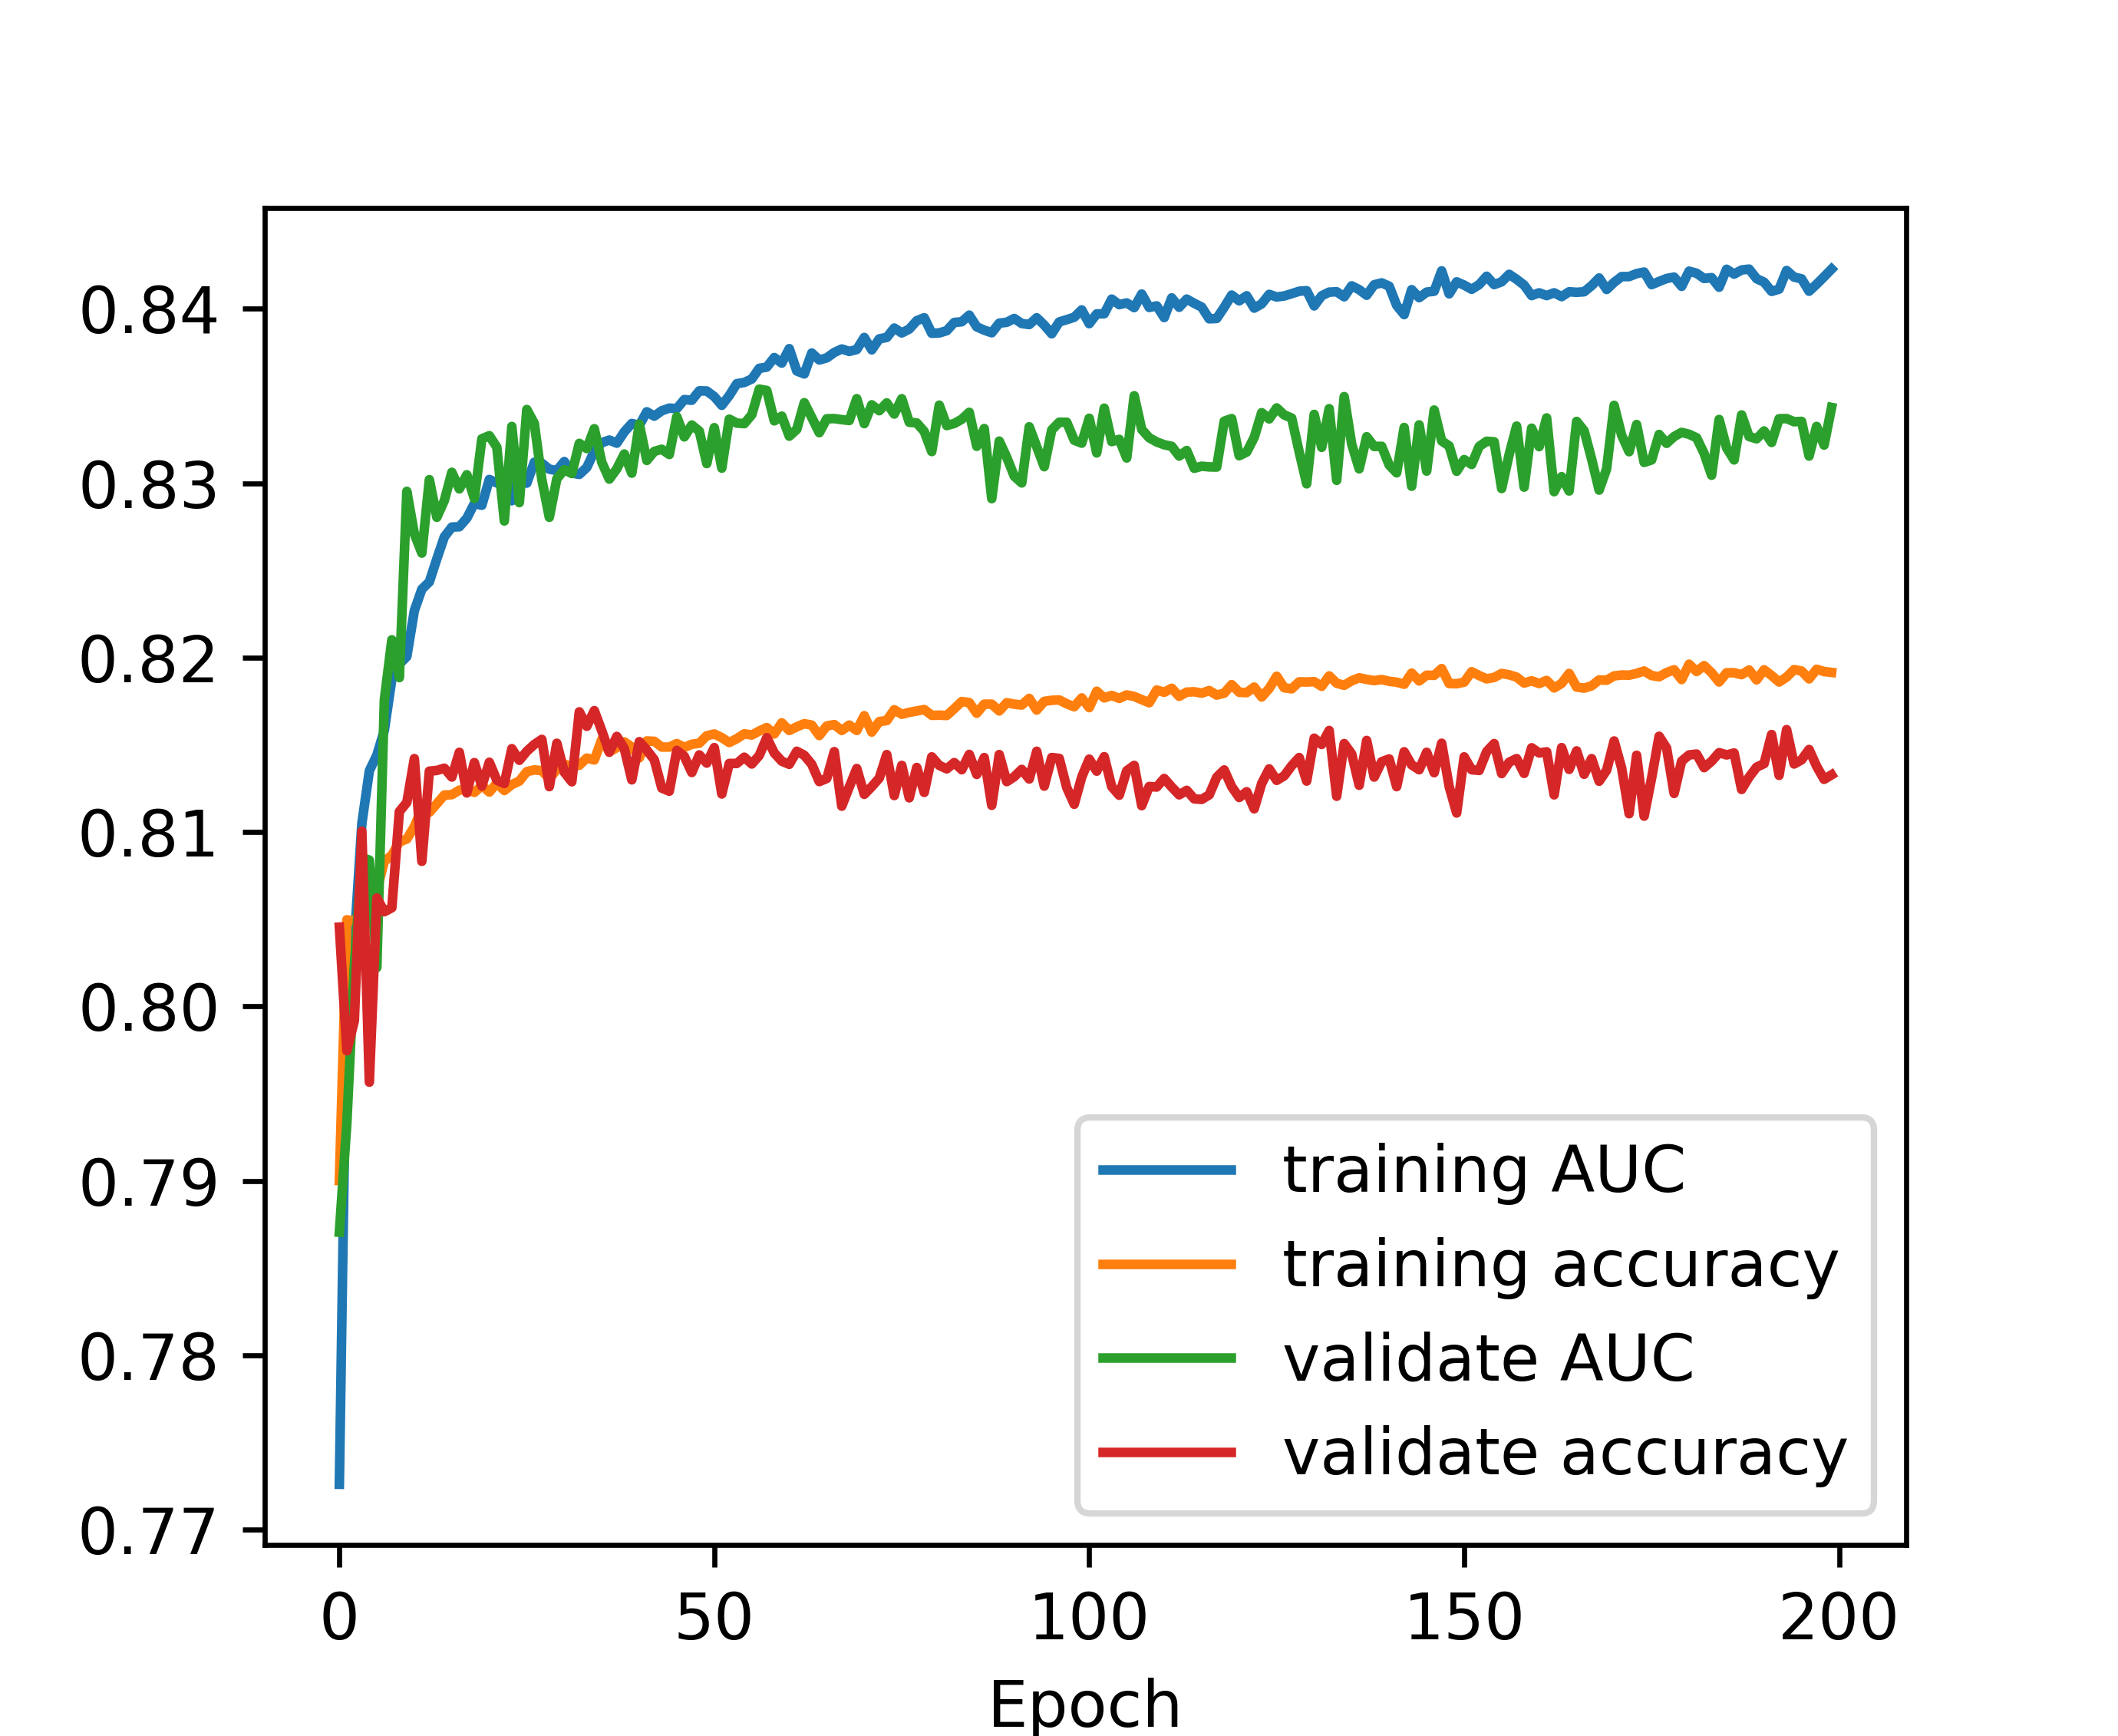
\includegraphics[width=0.9\textwidth]{ch3-train-acc.png}
    \caption{The training acc/auc of proposed model}\label{fig:ch3-train-acc}
\end{figure}
%结果显示,经过约150个epoch的训练,模型的预测性能可以稳定收敛。

The results show that the model's prediction performance can converge stably after about 150 epochs of training.
\subsection{Result and Analysis}
%实验结果见表\cite{\ref{tbl:ch3-performance}},相比于其他模型,提出的模型的性能在关键指标accuracy和AUC取得了最优的指标。有两点原因,一是因为模型考虑了用户的额外特征,因此引入了新的影响因素,二是模型考虑了潜在概念之间的模型,并利用图状结构来表征这种联系,从而为模型引入了高阶的知识点关系特征。综上所述,模型为知识追踪任务引入了新的解释特征,因此在模型的最终性能指标上取得了较大的提升。
The experimental results are presented in \tblname{\ref{tbl:ch3-performance}}, and the performance of the proposed model achieves optimal metrics in key indicators Accuracy and AUC compared to other models. There are two reasons for this, one is because the model considers additional features of the user and therefore introduces new influencing factors, and the other is that the model considers the model between potential concepts and uses graph-like structures to characterize such connections, thus introducing higher-order knowledge point relationship features to the model. In summary, the model introduces new explanatory features for the knowledge tracing task and therefore achieves a large improvement in the model's final performance metrics.

\begin{table}[htb]
    \centering
    \caption{Performance comparison between baseline and proposed models}\label{tbl:ch3-performance}
    \begin{tabular}{cccc}
        \toprule
        Model    & ACC (\%)                    & AUC (\%)                   & Training time (sec) \\
        \midrule
        DKT      & \(76.99\pm 0.08 \)          & \(81.79\pm 0.09\)          & \(2,731\)           \\
        DKVMN    & \(75.63\pm 0.19 \)          & \(79.58\pm 0.27\)          & \(3,378\)           \\
        NPA      & \(77.09\pm 0.08\)           & \(81.81\pm 0.13\)          & \(3,872\)           \\
        SAKT     & \(76.37\pm 0.15\)           & \(80.77\pm 0.09\)          & \(4,367\)           \\
        \midrule
        Proposed & \(\mathbf{81.34\pm 0.25} \) & \(\mathbf{83.20\pm 0.25}\) & \(4,597\)           \\
        \bottomrule
    \end{tabular}
\end{table}

%而在模型训练耗时上,本模型由于需要额外的图信息传播过程,因此相较于原始DKVMN模型训练效率会有所降低,为了解决该问题,可以考虑将图传播的方式通过矩阵运算的方式来进行计算,可以充分利用计算设备并行计算的能力。
As for the model training time consumption, this model will have a reduced training efficiency compared to the original DKVMN model because of the additional graph information propagation process. To solve this problem, the graph propagation can be considered to be computed by means of matrix operations, which can make full use of the parallel computing capability of computing devices.
\section{Summary}
In this section, an improved GKVMN model based on DKVMN is proposed, which adds the ability to characterize the relationships between knowledge points to the model by transforming the storage module that characterizes the exercises' potential concepts into a graph structure. On the other hand, the model introduces the student's answer characteristics to introduce more influencing factors, thus enhancing the model's predictive capability. In addition, the value storage module of the model can be used as the student's knowledge point mastery representation, which can explicitly output the student's mastery of potential concepts, thus adding more recommended input features for the subsequent exercise recommendation.

The main contributions of this section are as follows.
\begin{enumerate}
    \item the graph structure is used to characterize the relationship between the potential concepts of the exercises, taking into account the impact of the increase in mastery of the relevant knowledge points on the overall knowledge mastery. A graph propagation calculation is used to characterize the change in the mastery of the relevant knowledge points.
    \item additional student characteristics are introduced as inputs to the model, which adds more predictors to the model and takes into account the impact of various situations on the final correctness of the answers.
    \item the knowledge mastery proficiency of the model can be output explicitly, which improves the interpretability of the model.
\end{enumerate}

%在实验阶段,首先对原始数据集进行数据清洗、格式转换,然后对数据集进行特征相关性分析,目标-特征相关性分析,选取最佳的学生答题特征作为额外的输入特征。然后与一系列baseline知识追踪模型进行性能对比。实验显示,提出的模型在各项指标上都优于基线模型。
In the experimental phase, the original dataset is first cleaned and formatted with data preprocessing methods. Then the dataset is analyzed with feature correlation analysis and target-feature correlation analysis to select the best student answer features as additional input features. Finally, the performance is compared with a series of baseline knowledge tracing models. The experiments show that the proposed model outperforms the baseline model in all metrics.
\chapter{Exercise Recommendation System Based on Knowledge State}

% **************************** Define Graphics Path **************************
\ifpdf
  \graphicspath{{Chapter4/Figs/Raster/}{Chapter4/Figs/PDF/}{Chapter4/Figs/}}
\else
  \graphicspath{{Chapter4/Figs/Vector/}{Chapter4/Figs/}}
\fi

\section{Research Motivation}

%随着当今技术的飞速发展,数据量也与日俱增,人们越来越感觉在海量数据面前束手无策。正是为了解决信息过载的问题,人们提出了推荐引擎技术。推荐系统通过用户的历史行为或者用户的兴趣偏好或者用户的人口统计学特征来送给推荐算法,然后推荐系统运用推荐算法来产生用户可能感兴趣的项目列表,同时用户对于搜索引擎是被动的。目前个性化推荐技术被广泛应用于各个行业,它大大节省了用户获取信息的成本,也方便了信息提供商对用户的定向信息推送,因此大大加速了社会的信息交流效率,从而推动了传媒、娱乐、教育等基于信息交流的行业的发展。在教育领域,推荐系统的应用仍停留在较为初级的阶段,很多情况下还依赖人工筛选教育资源进行推荐,这种推荐方式效率低、成效差,且出于成本的原因也无法覆盖到所有的学生。随着推荐系统技术的成功应用和教育行业的进一步成熟,将以往通过人工实现的教育资源推荐系统改用智能化技术来进行的阻力越来越小。在国家提倡智慧教育、精准教学、智慧学习的背景下,一款成熟的具备实用价值的自适应习题推荐系统成为教育业者的期待。

%本章的目的是基于前两个章节所挖掘出的习题知识点和知识状态进行习题推荐,其核心是基于学生的知识状态,寻找出对学生当前知识掌握度改善最大的习题进行推荐,即习题推荐以查漏补缺为目的。因此获取学生的知识状态和习题涉及的知识点是本章前提。但是目前的习题库往往过于庞大,因此,从海量的习题推荐资源中直接应用推荐算法会出现效率较低的情况,不利于商业化大规模部署。在匹配阶段,根据用户特征,从海量的习题库中,快速筛选出一部分潜在适合的习题作为粗筛集合。在排序阶段,将提出的推荐模型应用于粗筛习题集,输出一个按照优先级排序的推荐习题集列表。


With the rapid development of today's technology, the amount of data is increasing day by day, and people increasingly feel helpless in the face of massive amounts of data. It is precisely in order to solve the problem of information overload that people propose the recommendation engine technology. The recommendation system sends the recommendation algorithm to the recommendation algorithm through the user's historical behavior or the user's interest preferences or the user's demographic characteristics, and then the recommendation system uses the recommendation algorithm to generate a list of items that the user may be interested in. At the same time, the user is passive to the search engine. At present, personalized recommendation technology is widely used in various industries. It greatly saves the cost for users to obtain information, and it also facilitates information providers to push targeted information to users. Therefore, it greatly accelerates the efficiency of social information exchange, thereby promoting media, The development of industries based on information exchange, such as entertainment and education. In the education field, the application of the recommendation system is still at a relatively primitive stage. In many cases, it still relies on manual screening of educational resources for recommendation. This recommendation method is inefficient, poorly effective, and cannot cover all of them due to cost reasons. student. With the successful application of the recommendation system technology and the further maturity of the education industry, the resistance to the use of intelligent technology in the education resource recommendation system implemented manually in the past is becoming less and less. In the context of the country's promotion of smart education, precise teaching, and smart learning, a mature and practical self-adaptive exercise recommendation system has become the expectation of the education industry. For the purpose of improving education and teaching, this chapter proposes an exercise recommendation model based on students' knowledge mastery.

The purpose of this chapter is to recommend exercises based on the knowledge points and knowledge status of the exercises excavated in the first two chapters. The core is to find the exercises that improve the students' current knowledge mastery the most for recommendation based on the student's knowledge status, that is, exercises It is recommended to check for omissions and fill vacancies. Therefore, acquiring the knowledge status of students and the knowledge points involved in the exercises is the premise of this chapter. However, the current exercise database is often too large. Therefore, directly applying the recommendation algorithm from the massive exercise recommendation resources will have low efficiency and is not conducive to commercial large-scale deployment. Therefore, this paper proposes a recommendation model based on two stages of matching and ranking. n the matching stage, according to the user's characteristics, a part of the potentially suitable exercises is quickly screened out from the massive exercise library as a coarse sieve set, and then based on the coarse sieve set, the proposed recommendation algorithm model is applied to recommend exercises. In the matching stage, according to the characteristics of users, a part of the potential suitable exercises can be quickly screened out as a coarse screening set from the massive exercise library. In the ranking stage, the proposed recommendation model is applied to the coarse screening exercise set, and a list of recommended exercise sets sorted by priority is output.

\section{Proposed Model}
%推荐系统本质上就是一个信息过滤系统,目前常见的工业推荐系统往往具备若干过滤、排序等多个环节,每个环节逐层过滤,最终从海量的物料库中筛选出几十个用户可能感兴趣的物品推荐给用户。推荐系统作为一种解决用户信息过载的方式,通过分析用户的行为数据、历史记录等等来建立用户画像,再根据用户个性化模型推荐他们感兴趣的推荐项。在传统的推荐系统中,采用的模型一般是基于矩阵分解模型的模型,例如SVD+、BPR、 因子分解机(FM)等等,随着深度学习研究的兴起,基于深度学习模型的深度推荐模型技术也逐渐发展起来。目前已经有一些模型用深度学习来表征推荐项目的高阶特征,例如Deep&Wide、DeepCross、DeepFM等。深度推荐模型由于其对隐藏特征的建模能力,在推荐精度上有部分提升。但是深度推荐算法往往会产生较大的计算开销,直接应用全阶段深度推荐模型不切实际,因此可以采用基于匹配-排序双阶段的推荐模型,利用开销较低的匹配算法来进行推荐项近似筛选,产生候选推荐项目集合。匹配阶段的核心任务是从海量习题库中快速获取一批候选习题库,要求是快和尽可能的准。这一层通常有丰富的策略和算法,用来确保多样性,为了更好的推荐效果,需要对算法进行速度与精度的权衡。在排序阶段再应用推荐算法进行推荐项的打分或者优先级排序,进行精细化排序。它会利用习题、用户以及习题-用户交叉特征,然后通过复杂的机器学习或者深度学习模型进行打分排序,这一层的特点是计算复杂但是结果更精准。

A recommendation system is essentially an information filtering system. Currently, common industrial recommendation systems often have a number of filters, ranking and other multiple links, each filtering layer by layer, and eventually filtering out dozens of items that may be of interest to users from a massive library of materials to recommend to users. As a method to solve the overload of user information, the recommendation system builds user portraits by analyzing user behavior data, historical records, etc., and then recommends recommendation items that they are interested in based on the user's personalized model. In traditional recommendation systems, the models used are generally models based on matrix factorization models, such as BPR\cite{rendle2012bpr}, factorization machines (FM)\cite{koren2008factorization} and weighted matrix factorization(WMF)\cite{hu2008collaborative}, etc. As deep learning research gradually becomes popular, deep recommendation model technology based on deep learning models is also gradually developed. There are already some models that use deep learning to characterize the high-level features of recommended items, such as Deep\&Wide\cite{cheng2016wide}, DeepCross\cite{shan2016deep}, DeepFM\cite{guo2017deepfm}, etc. The deep recommendation model has a partial improvement in recommendation accuracy due to its ability to model hidden features. However, in-depth recommendation algorithms often incur large computational overhead, and it is impractical to directly apply the full-stage in-depth recommendation model. Therefore, a recommendation model based on a matching-ranking two-stage can be used, and a matching algorithm with lower overhead can be used to approximate recommendation items. , Generate a set of candidate recommendation items. The core task of the matching phase is to quickly obtain a pool of candidate exercises from a massive library of exercises, and the requirement is to be fast and as accurate as possible. This layer usually has a rich set of strategies and algorithms used to ensure diversity, and the algorithms need to be traded off between speed and accuracy for better recommendation results. The recommendation algorithm is then applied in the ranking stage to score or prioritize the recommended items for refined ranking. It will use the exercise, user, and exercise-user crossover features, and then perform scoring and ranking by complex machine learning or deep learning models, which is characterized by a complex calculation but more accurate results at this layer.

\subsection{Algorithm Overview}
%本章提出一个基于Matching-Ranking-Feedback三个阶段的数学习题推荐模型。考虑到待推荐的习题库较为庞大,因此先采用多因素习题匹配的方式筛选出习题候选集合,然后基于提出的深度推荐模型进行习题推荐优先级排序,最后在反馈阶段由用户打分,判定推荐的合理性。
This chapter proposes a recommendation model based on three stages of Matching-Ranking-Feedback. It addresses the problem of low recommendation efficiency caused by too large exercise database, and proposes a collaborative filtering-based exercise matching screening algorithm to filter out a small scale The candidate set of exercises.

% 分为以下几个部分:第一部分为召回部分,
%1. 练习候选生成。这部分的作用是生成一系列符合学生当前学习状态的练习,并快速筛选出一组初步的练习,后续部分将从这组练习中生成最合适的N个练习,并通过协同过滤算法进行排序。它参考youtube推荐系统设计了一个多层MLP网络。它将知识跟踪生成的学生学习状态嵌入向量与学生的问题记录嵌入、个性化信息等并联作为输入。经过一系列的ReLU网络,然后通过softmax归一化输出所有候选练习的概率分布。
%2. 第二部分该部分用与上一部分类似的神经网络架构,实现了对推荐试题的排序。它的输入是用户的知识结构,最近练习,以及相似用户的常见练习题。

This chapter proposes an adaptive test question recommendation method combining graph neural network knowledge tracking and collaborative filtering. This method uses the GAT knowledge tracking model designed in the previous chapter to model the student's knowledge state, and uses the graph neural network clustering method to cluster the test questions based on knowledge points, so as to obtain a series of related exercise. The first part is the matching part, i.e., candidate test generation, which generates a series of similar exercises, and this is done by clustering the test questions through graph neural networks, which apply graph clustering methods to cluster the test questions based on knowledge points in a reasonable way. The second part is the ranking part, which combines the knowledge state of students obtained from the knowledge tracking system with co-filtering.
\begin{enumerate}
  \item Exercise candidate generation: The role of this part is to generate a series of exercises that match the student's current learning state, and quickly filter out a preliminary set of exercises, and the subsequent part will generate the most suitable N exercises from this set and sort them by collaborative filtering algorithms. It designs a multi-layer MLP network with reference to the youtube recommendation system. It concatenates the student learning state embedding vector generated by knowledge tracking with the student's problem record embedding, personalized information, etc.\ as input. After a series of ReLU networks and then output a probability distribution over all candidate exercises by softmax normalization.
  \item Ranking: This part is to generate Top N recommendation exercise. It implements the ranking of the recommended test questions using a neural network architecture similar to that of the previous section. Its inputs are the user's knowledge structure, recent exercises, and common practice questions from similar users.
\end{enumerate}

The structure of the recommendation system is like \figurename{\ref{fig:ch4-fig0}}

\begin{figure}[h]
  \centering
  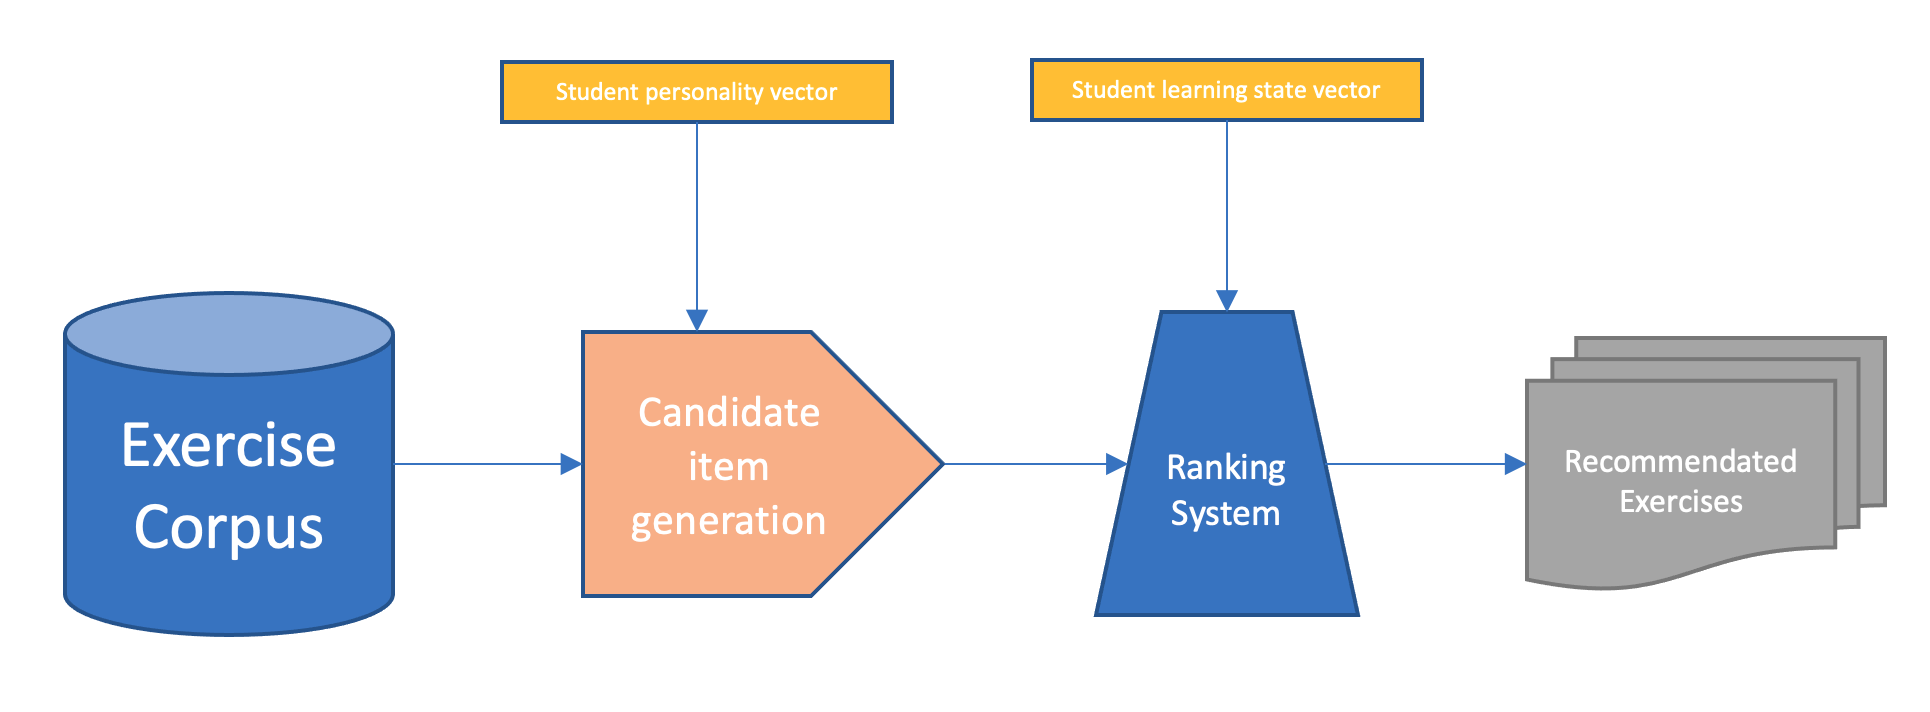
\includegraphics[width=1.0\textwidth]{ch4-fig1.png}
  \caption{The Architecture of Recommendation System}\label{fig:ch4-fig0}
\end{figure}

\subsection{Matching Stage}
%本推荐模型的第一阶段为召回,召回层的目的是在确保一定准确度的情况下快速筛选出候选的推荐习题集合。在上一个知识追踪模型中,已经获得了用户的知识状态表征以及历史知识状态。在习题知识点标注模块中,获得了经过标注知识点的习题。与新闻推荐算法等相比,习题和用户的知识状态都是较为规则化的向量数据,计算习题、用户以及习题-用户交叉特征相似度相对简单,可以利用相似度来应用协同过滤算法作为一种召回策略。用户的历史回答错误错习题、统计的容易答错的习题等对于学生检查知识掌握完整度以及更正误区具有较大意义,因此筛选错误率较高的习题也可以作为一种召回策略。在召回阶段,可以应用不同的自适应参数或算法来控制候选习题集的大小,以适配原始数据集和推荐系统部署环境。

%

The first stage of the recommendation model is matching. The purpose of the matching layer is to quickly screen out a set of candidate recommended exercises while ensuring a certain degree of accuracy. In the previous knowledge tracking model, the user's knowledge status representation and historical knowledge status have been obtained. In the exercise knowledge point labeling module, the exercises with marked knowledge points are obtained. Compared with recommendation algorithms such as news, the exercises and the user's knowledge state are more regular vector data, so similarity calculations and collaborative filtering algorithms can be applied to the candidate problem sets that are of potential interest to the object to be recommended. In the matching phase, different adaptive parameters or algorithms can be applied to control the size of the candidate set of exercises to fit the original dataset and the recommendation system deployment environment.

In the matching phase, due to the large amount of data, the algorithm of Collaborative Filtering (CF)\cite{salakhutdinov2007restricted} can achieve half the result with twice the effort. It only needs to calculate the similarity of students' knowledge states \(h^\prime \) with other students who have similar knowledge states \(h\).

Collaborative Filtering, the most classic type of recommendation algorithm, includes both online collaborative and offline filtering. The so-called online collaborative is to find items that users may like through online data, while offline filtering is to filter out data that are not worth recommending, such as data with low recommendation value ratings, or data that users have already purchased despite high recommendation values. The model of collaborative filtering is generally m recommended items, m users' data, only some users and some data are rated between the data, other parts of the rating is blank, at this time we want to use the existing part of the sparse data to predict the rating relationship between those blank items and data to find the highest rated items recommended to users.

Generally speaking, there are three types of collaborative filtering recommendations. The first one is user-based collaborative filtering, the second one is item-based collaborative filtering, and the third one is model-based collaborative filtering.


\subsubsection{Student Similarity Calculation}
The purpose of collaborative filtering is to recommend recommended items of users similar to the target user to the user. The user-based collaborative filtering algorithm is discovered through historical behavior data of users, and measures and scores these preferences. Set the similarity of users through a given algorithm, and make recommendations among users who have the same preferences.

User-based collaborative filtering mainly considers the similarity between users and users. As long as we find out the items that similar users like and predict the target users' ratings of the corresponding items, we can find the items with the highest ratings and recommend them to users. The item-based collaborative filtering is similar to the user-based collaborative filtering, except that we turn to find the similarity between items and users, and only if we find the ratings of certain items by target users, then we can predict similar items with high similarity and recommend the highest rated similar items to users. For example, if you buy a machine learning related book online, the website will immediately recommend a bunch of machine learning, big data related books to you, and the idea of collaborative filtering based on items is obviously used here.

Similar statistics are used to get neighboring users with similar hobbies or interests, so we can use the obtained user's knowledge state embedding \(h_t\) from the previous knowledge tracking module, which can be used as the basis for calculating the similarity. The first step is to find other users who are similar to the new user based on their historical behavior information; at the same time, to predict the items that the current new user may like based on the evaluation information of these similar users on other items. Given the user rating data matrix R, the user-based collaborative filtering algorithm needs to define the similarity function \(s : U \times U \to R\) to calculate the similarity between users, and then calculate the recommendation results based on the rating data and the similarity matrix. We can use the cosine similarity to calculate this value.

\begin{align}
  s(u, v)=\frac{h_{u} \cdot h_{v}}{\|h_{u}\|_{2}\|h_{v}\|_{2}}
\end{align}
where \(h_u\) and \(h_v\) represent the knowledge mastery state of user \(u\) and \(v\).
We can obtain the exercise recommendation history \(\mathcal{H}\) of user B, which is closest to user A to be recommended, and then use the exercises in \(\mathcal{H}\) as a rough set as the next sorted list of exercises.

\subsubsection{Exercise Filtering System}
Through the previous section, we calculated the similarity of students, which comprehensively considers students' current knowledge proficiency, students' personalized information and so on. Next, we need to use the collaborative filtering algorithm to generate a rough recommended set of exercises \(S_{raw}\).

When the recommendation system is running, the system will record the students' question records. After calculating the similarity of the students, they can be sorted according to the similarity. Given a threshold, list the students whose similarity is greater than the threshold, and divide the students according to the list. The exercises corresponding to the problem record are added to \(S_{raw}\).

The algorithm is as~\ref{alg:EF}:
\begin{algorithm}[h]
  \caption{Exercise Filtering Algorithm}\label{alg:EF}
  \begin{algorithmic}
    \REQUIRE~~\\
    The target student \(s_i\); \\
    The student represent matrix, \(S=\{s_0,s_1,\ldots,s_N\} \);\\
    The log of recommendation \(L=\{L_0,L_1,\ldots,L_N\} \) \\
    The log-exercise relation: \(L_i=\{E_0,\ldots,E_{|L_i|}\} \) \\
    The filtering thread \(T\);
    \ENSURE~~\\ %算法的输出:Output
    The filtered exercise set \(S=\{E_{s_0},\ldots,E_{s_N}\} \)
    \STATE~Calculate the similarity between \(s_i\) and other students \(Sim\)
    \STATE~Sort \(Sim\) and get the top \(T\) results \(R=\{s_{r_0},\ldots,s_{r_T}\} \);
    \STATE~Aggregate the exercises log of students in \(R\), get exercise set \(S\)
    \RETURN~\(S\); %算法的返回值
  \end{algorithmic}
\end{algorithm}




\subsection{Ranking Stage}
%本节我们设计了一个基于MLP的试题排序模型,该模型输入学生的知识状态向量$h_t$,以及通过序列嵌入学习的知识状态改变向量$d_h$,以及习题的知识点标注向量。

In the previous step we obtained a list of recommended exercises for similar students by collaborative filtering in the matching phase, and in this phase, a ranking of the exercises is needed to further reduce the amount of recommendations and give the ranking sequence of exercise. In this section, we design an MLP-based test ordering model. The model inputs the student's knowledge state vector \(h_t\), the knowledge state change vector \(d_h\) learned through sequence embedding, and the knowledge point labeling vector of the exercises. The architecture is like \figurename{\ref{fig:ch4-fig3}}.


\begin{figure}[h]
  \centering
  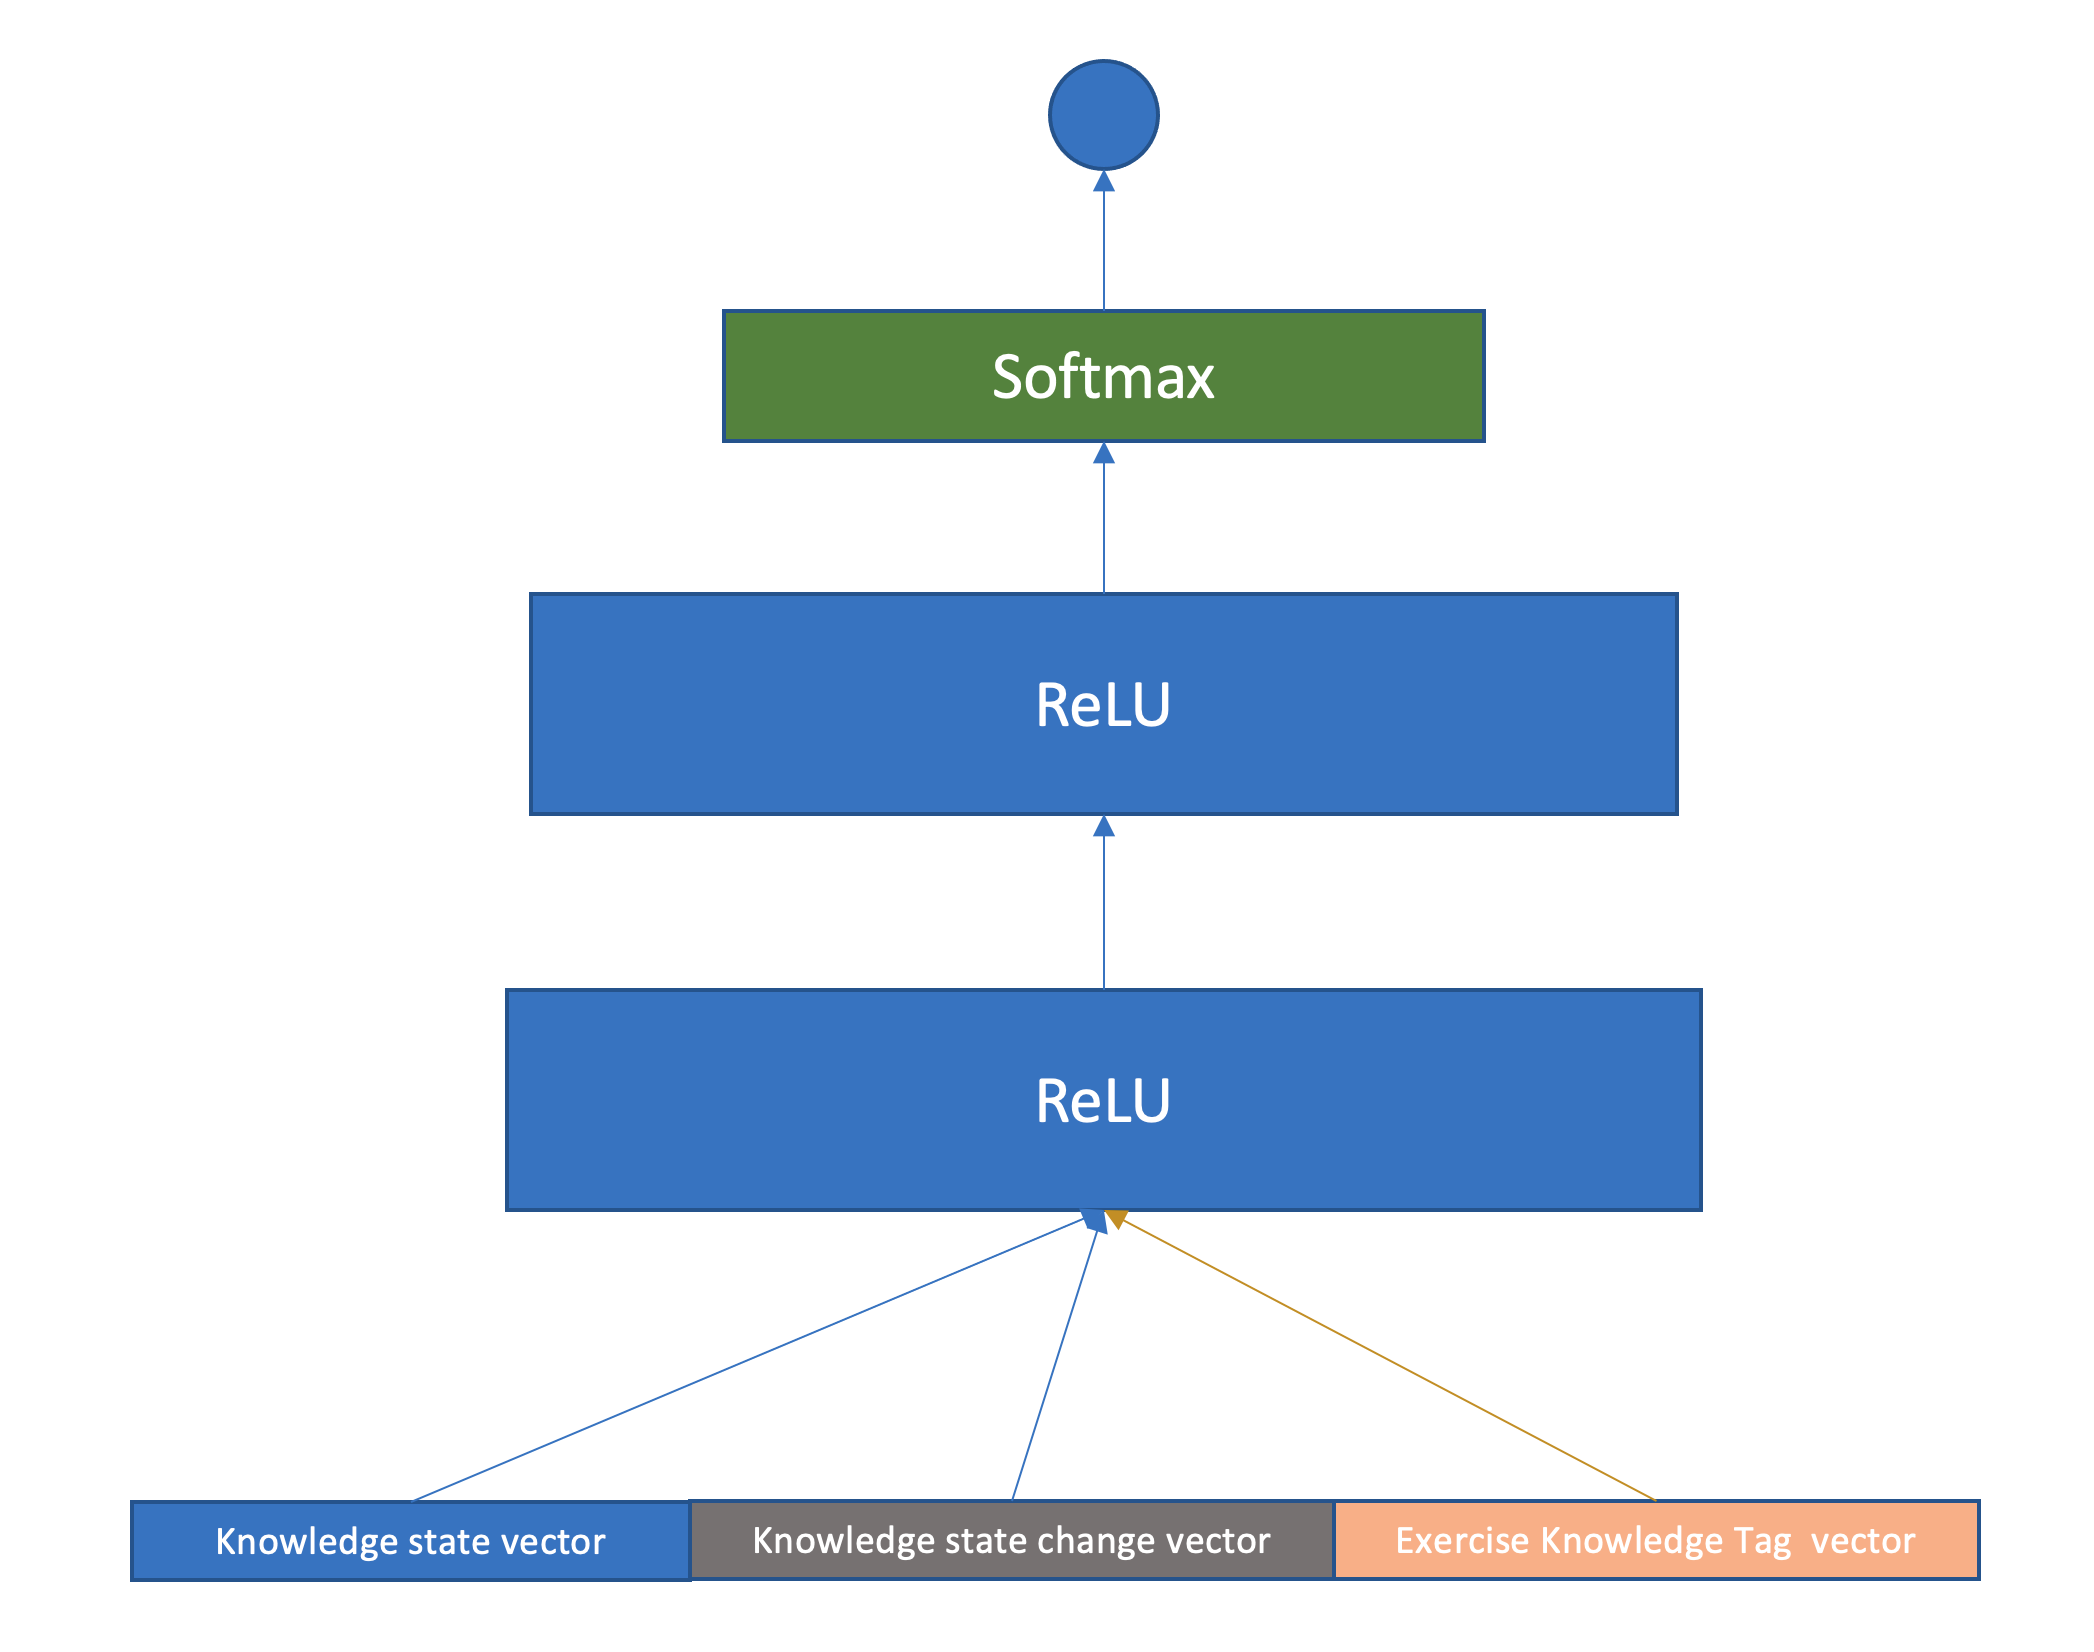
\includegraphics[width=1.0\textwidth]{ch4-fig3.png}
  \caption{The Architecture of Recommendation System}\label{fig:ch4-fig3}
\end{figure}

The model is a three-layer multi-layer perceptron, with two fully connected layers in the middle, and the output layer uses softmax to output the probabilities of exercise recommendation. The input layer inputs the student's knowledge state vector, knowledge state change vector and exercise knowledge point label vector. The model is a three-layer multi-layer perceptron, with two fully connected layers in the middle, and the output layer uses softmax to output the probabilities of exercise recommendation. The input layer inputs the student's knowledge state vector, knowledge state change vector and exercise knowledge point label vector. The loss function is:
\begin{align}
  \mathcal{L}=\sum_{i=1}^{T} y_i \log (\text{sigmoid}(\hat{y}_i))+(1-y_i ) \log (1-\text{sigmoid}(\hat{y}_i))
\end{align}
where \(\hat{y}_i\) is the output value, \(y_i\) is actual recommended weights for the exercises.

After training the model, sort the output values, and the sorted list is the recommended problem set.
%在训练好模型之后,将输出值进行排序,排序的列表即为推荐的习题集。


\section{Experiment}
%本模型的核心思想是为学生查漏补缺,因此,在学生的知识状态一定的情况下,尽量给学生推荐对其知识掌握情况带来正向收益最大的习题。
\subsection{Dataset}
%考虑到本推荐系统需要立足于学生的知识状态针对习题进行推荐。目前市面上并没有

\section{Summary}
%本节提出了一个基于召回-排序的双阶段推荐系统框架,在召回阶段,采用了协同过滤的方式,排序阶段,则采用了多层感知机,来对学生知识状态-习题知识点进行建模,同时考虑到学生的学习速度即知识状态改变,输出习题与当前知识状态匹配度。
This section proposes a two-stage recommendation system framework based on matching-ranking. In the matching stage, collaborative filtering is used, and in the ranking stage, multi-layer perceptron are used to model students' knowledge state-exercise knowledge points. At the same time, taking into account the student's learning speed, that is, the change of knowledge state, the output exercises match the current knowledge state.
%\chapter{My Third Chapter}

% **************************** Define Graphics Path **************************
\ifpdf
    \graphicspath{{Chapter5/Figs/Raster/}{Chapter5/Figs/PDF/}{Chapter5/Figs/}}
\else
    \graphicspath{{Chapter5/Figs/Vector/}{Chapter5/Figs/}}
\fi

\section{First Section of the Third Chapter}
And now I begin my third chapter here \dots

And now to cite some more people~\citet{Rea85,Ancey1996}

\subsection{First Subsection in the First Section}
\dots and some more

\subsection{Second Subsection in the First Section}
\dots and some more \dots

\subsubsection{First Subsub Section in the Second Subsection}
\dots and some more in the first subsub section otherwise it all looks the same
doesn't it? well we can add some text to it \dots

\subsection{Third Subsection in the First Section}
\dots and some more \dots

\subsubsection{First Subsub Section in the Third Subsection}
\dots and some more in the first subsub section otherwise it all looks the same
doesn't it? well we can add some text to it and some more and some more and
some more and some more and some more and some more and some more \dots

\subsubsection{Second Subsub Section in the Third Subsection}
\dots and some more in the first subsub section otherwise it all looks the same
doesn't it? well we can add some text to it \dots

\section{Second Section of the Third Chapter}
and here I write more \dots

\section{The Layout of Formal Tables}
This section has been modified from ``Publication quality tables in \LaTeX*''
 by Simon Fear.

The layout of a table has been established over centuries of experience and
should only be altered in extraordinary circumstances.

When formatting a table, remember two simple guidelines at all times:

\begin{enumerate}
  \item Never, ever use vertical rules (lines).
  \item Never use double rules.
\end{enumerate}

These guidelines may seem extreme but I have
never found a good argument in favour of breaking them. For
example, if you feel that the information in the left half of
a table is so different from that on the right that it needs
to be separated by a vertical line, then you should use two
tables instead. Not everyone follows the second guideline:

There are three further guidelines worth mentioning here as they
are generally not known outside the circle of professional
typesetters and subeditors:

\begin{enumerate}\setcounter{enumi}{2}
  \item Put the units in the column heading (not in the body of
          the table).
  \item Always precede a decimal point by a digit; thus 0.1
      {\em not} just .1.
  \item Do not use `ditto' signs or any other such convention to
      repeat a previous value. In many circumstances a blank
      will serve just as well. If it won't, then repeat the value.
\end{enumerate}

A frequently seen mistake is to use `\textbackslash begin\{center\}' \dots `\textbackslash end\{center\}' inside a figure or table environment. This center environment can cause additional vertical space. If you want to avoid that just use `\textbackslash centering'


\begin{table}
\caption{A badly formatted table}
\centering
\label{table:bad_table}
\begin{tabular}{|l|c|c|c|c|}
\hline
& \multicolumn{2}{c}{Species I} & \multicolumn{2}{c|}{Species II} \\
\hline
Dental measurement  & mean & SD  & mean & SD  \\ \hline
\hline
I1MD & 6.23 & 0.91 & 5.2  & 0.7  \\
\hline
I1LL & 7.48 & 0.56 & 8.7  & 0.71 \\
\hline
I2MD & 3.99 & 0.63 & 4.22 & 0.54 \\
\hline
I2LL & 6.81 & 0.02 & 6.66 & 0.01 \\
\hline
CMD & 13.47 & 0.09 & 10.55 & 0.05 \\
\hline
CBL & 11.88 & 0.05 & 13.11 & 0.04\\
\hline
\end{tabular}
\end{table}

\begin{table}
\caption{A nice looking table}
\centering
\label{table:nice_table}
\begin{tabular}{l c c c c}
\hline
\multirow{2}{*}{Dental measurement} & \multicolumn{2}{c}{Species I} & \multicolumn{2}{c}{Species II} \\
\cline{2-5}
  & mean & SD  & mean & SD  \\
\hline
I1MD & 6.23 & 0.91 & 5.2  & 0.7  \\

I1LL & 7.48 & 0.56 & 8.7  & 0.71 \\

I2MD & 3.99 & 0.63 & 4.22 & 0.54 \\

I2LL & 6.81 & 0.02 & 6.66 & 0.01 \\

CMD & 13.47 & 0.09 & 10.55 & 0.05 \\

CBL & 11.88 & 0.05 & 13.11 & 0.04\\
\hline
\end{tabular}
\end{table}


\begin{table}
\caption{Even better looking table using booktabs}
\centering
\label{table:good_table}
\begin{tabular}{l c c c c}
\toprule
\multirow{2}{*}{Dental measurement} & \multicolumn{2}{c}{Species I} & \multicolumn{2}{c}{Species II} \\
\cmidrule{2-5}
  & mean & SD  & mean & SD  \\
\midrule
I1MD & 6.23 & 0.91 & 5.2  & 0.7  \\

I1LL & 7.48 & 0.56 & 8.7  & 0.71 \\

I2MD & 3.99 & 0.63 & 4.22 & 0.54 \\

I2LL & 6.81 & 0.02 & 6.66 & 0.01 \\

CMD & 13.47 & 0.09 & 10.55 & 0.05 \\

CBL & 11.88 & 0.05 & 13.11 & 0.04\\
\bottomrule
\end{tabular}
\end{table}

\chapter{Conclusion and Future Work}
%在本文中,设计了一个基于图神经网络、Attention-based Bi-LSTM、Transformer以及协同过滤等算法的习题推荐系统。该系统分为三个模块,分别为习题知识点挖掘模块、知识追踪模块和习题推荐模块。习题知识点挖掘模块可以未标注知识点的习题进行知识点标注,并将标注知识点的习题作为知识追踪的输入数据。知识追踪模块追踪学生的做题记录,从而跟踪学生的知识状态。习题推荐模块则结合学生的知识状态和习题标签信息,进行针对性的习题推荐。

%在未来的工作中,可以结合其他的图神经网络模型或者加入一些记忆力机制来解决模型的序列性问题。
In this article, an exercise recommendation system based on graph neural network, Attention-based Bi-LSTM, Transformer, and collaborative filtering algorithms are designed. The system is divided into three modules: the exercise knowledge point mining module, knowledge tracking module, and exercise recommendation module. The exercise knowledge point mining module can mark the exercises' knowledge points without the knowledge points and use the marked knowledge points as the input data for knowledge tracking. The knowledge tracking module tracks the students' question records, thereby tracking the students' knowledge status. The exercise recommendation module combines students' knowledge status and exercise label information to make targeted exercise recommendations.

%在知识点标注模块中,采用了图卷积神经网络来训练标签标注分类器。通过Bi-LSTM来挖掘习题文本信息,将习题文本嵌入作为标签分类器组的输入,输出一组标签的分类结果。经过实验验证,该模型对于高中数学习题具有良好的分类效果,对于现有的模型性能上有一定提升。在未来的工作中,可以考虑用Transformer来取代Bi-LSTM模型或者用BERT来训练习题文本嵌入来达到更精确的分类效果。

In the knowledge point annotation module, a graph convolutional neural network is used to train the label annotation classifier. Use Bi-LSTM to mine the exercise text information, embed the exercise text as the label classifier group's input, and output a set of label classification results. Experiments show that the model has a good classification effect for high school math learning problems and has a specific improvement in existing models' performance. In future work, a Transformer can be applied to replace the Bi-LSTM model or BERT to train exercise text embedding to achieve more accurate classification results.

%在知识追踪模块中,采用了图注意力网络来进行习题知识关系嵌入学习,将嵌入向量通过基于Transformer的Encoder模型来输出一个知识状态向量,再将习题嵌入向量与知识状态向量作为基于Transformer的Decoder模型的输入,输出对于下一道习题的答题情况预测。经过实验验证,该模型对于知识关系简单与知识关系复杂的数据集都具有较好的预测性能。后续可以考虑采用不同的图神经网络模型来增加学习效率,或者采用更多的习题信息来学习习题知识嵌入。

In the knowledge tracking module, a graph attention network is used to learn exercises' knowledge relationships. The embedding vector is output through the Transformer-based Encoder model to output a knowledge state vector, and then the exercise embedding vector and the knowledge state vector are used as the Transformer-based Decoder. The input and output of the model predict the answer to the next exercise. After experimental verification, the model has good predictive performance for data sets with complex and straightforward knowledge relationships. Later, consider using different graph neural network models as an optional method to increase learning efficiency or use more exercise information to learn exercise knowledge embedding.

%在习题推荐模块中,提出一个基于Matching-Ranking双阶段的数学习题推荐模型。其中第一阶段的Matching模型为一个多路习题推荐项匹配模型,该模型采用了基于协同过滤、热门度、用户偏好等多个子召回策略用于分别生成习题推荐候选集合,然后在融合阶段将这些候选集合进行加权融合,形成一个最终的融合习题推荐候选集合。在排序阶段,将Matching阶段获取的习题候选集合中的每个习题输入到知识追踪习题进行正确率预测,将最容易出错的习题的作为优先级最高的推荐项,按照此策略生成推荐习题集。

In the exercise recommendation module, a two-stage Matching-Ranking based mathematical exercise recommendation model is proposed. The Matching model in the first stage is a multiplexed exercise recommendation item matching model, which employs multiple sub-matching strategies based on collaborative filtering, popularity, user preferences for generating exercise recommendation candidate sets separately, and then these candidate sets are weighted and fused in the fusion stage to form a final fused exercise recommendation candidate set. In the ranking phase, each exercise in the set of exercise candidates obtained in the Matching phase is input to the knowledge tracking exercise for correctness prediction, and the most error-prone exercises are used as the recommendation item with the highest priority, and the recommended set of exercises is generated according to this strategy.

%在未来的工作中,对于习题知识点标注模型,可以应用目前较为热门的预训练模型例如BERT,GPT等来进行嵌入学习和命名试题挖掘等工作,这样可以对于习题文本进行更深层次的语义理解,取得更好的效果。对于知识追踪模型,可以考虑应用其他图神经网络模型进行习题-知识点图嵌入学习,将知识点的关系定量化来建模,另外可以设计显式知识点掌握度矩阵来可视化学生对于具体知识点的掌握情况。对于习题推荐模型,可以应用神经网络模型来自适应调整各个召回策略的超参数,降低人工调参成本。

In future work, for the exercise knowledge point labeling model, the popular pre-training models such as BERT, GPT can be applied for embedding learning and named test mining, which can provide a deeper semantic understanding of the exercise text and achieve better results. For the knowledge tracking model, applying other graphical neural network models can be an option to embed the learning of exercise - knowledge point graphs to quantify the relationship of knowledge points to the model. An explicit knowledge mastery matrix can be designed to visualize students' mastery of specific knowledge points. For the exercise recommendation model, neural network models can adaptively adjust each matching strategy's hyperparameters to reduce manual tuning costs.



% ********************************** Back Matter *******************************
% Backmatter should be commented out, if you are using appendices after References
%\backmatter

% ********************************** Bibliography ******************************
\begin{spacing}{0.9}

% To use the conventional natbib style referencing
% Bibliography style previews: http://nodonn.tipido.net/bibstyle.php
% Reference styles: http://sites.stat.psu.edu/~surajit/present/bib.htm

\bibliographystyle{apalike}
%\bibliographystyle{unsrt} % Use for unsorted references
%\bibliographystyle{plainnat} % use this to have URLs listed in References
\cleardoublepage
\bibliography{References/references} % Path to your References.bib file


% If you would like to use BibLaTeX for your references, pass `custombib' as
% an option in the document class. The location of 'reference.bib' should be
% specified in the preamble.tex file in the custombib section.
% Comment out the lines related to natbib above and uncomment the following line.

%\printbibliography[heading=bibintoc, title={References}]


\end{spacing}

% ********************************** Appendices ********************************

\begin{appendices} % Using appendices environment for more functunality

% ************************** Thesis Abstract *****************************
% Use `abstract' as an option in the document class to print only the titlepage and the abstract.

%Please list 3-5 keywords, and replace them with "keyword1", "keyword2", "keyword3",...
\begin{abstract}{Graph Neural Network}{Knowledge Point Labeling}{knowledge tracing}{Recommended Exercises}{}
	After 2010, artificial intelligence technology has gradually become a popular research topic in computer technology. In particular, the advent of AlphaGo has aroused great concern in the industry for the prospect of artificial intelligence. This has brought about the industry's explosive development and raised a large number of research topics. In artificial intelligence-related research, various algorithm innovations, theoretical breakthroughs, and model applications are emerging one after another, laying the foundation for various industries' intelligence. The application of artificial intelligence technology in the field of education has also given birth to the emergence of the concept of intelligent education. Among them, adaptive learning is one of the popular application fields in intelligent education~\cite{chen2018recommendation}. Adaptive learning models generally track students' learning status by combining extensive data analysis of massive student group learning data and precise data analysis of target student individual data, targeting personalizing the learning path according to the students' individual characteristics and the proficiency of knowledge mastery~\cite{soltani2019adaptive}. Adaptive learning technology can use automated machine learning algorithms to complete student evaluation and teaching plans that required much manual labor in the past, which can systematically alleviate the current scarcity and uneven distribution of domestic educational resources and reduce the burden on education practitioners and students. It also has excellent development prospects and commercial value. More and more artificial intelligence research teams and intelligent education technology companies on the market focus on developing and applying adaptive learning tools. Some smart educational technology companies have used adaptive learning as the core function or main selling point of their products. Adaptive educational technology can comprehensively analyze students' individual-level learning ability, knowledge proficiency, group-level popular learning resources, error-prone questions, etc. The most suitable learning path and learning resources such as exercises, materials, and knowledge points can be pushed to the student. According to the students ' knowledge status, the system automatically adjusts the knowledge focus of the pushed learning resources to prevent the repetitive practice of already mastered knowledge points or lack of practice of unmastered knowledge points.

	On the one hand, teachers can analyze the whole class's knowledge mastery proficiency based on the system's data or visual charts to create a learning status assessment report for each student and adaptively adjust the overall teaching plan. On the other hand, students can use the system to analyze their knowledge weaknesses and target appropriate exercises. Thus, adaptive learning is one of the potentially feasible solutions to the ``automatic assessment of students'' knowledge mastery status and instructional program generation'' in online education.

	The purpose of this paper is to propose a knowledge-tracing-based model for recommending high school mathematics exercises, using the subject of high school mathematics as the primary research context. In high school mathematics, practice exercises are the principal means for students to improve their learning ability. However, in the current high school mathematics teaching, teachers or students need to find suitable exercises to practice from a vast library of exercises, which are often too large, highly repetitive, and confusingly organized. There are many low-quality unlabeled exercises in the exercise bank, which need to be manually labeled with knowledge points. Some students study through excessive exercises tactic, but this is less efficient and often results in repetition of familiar knowledge and avoidance of unfamiliar knowledge. To improve the effectiveness of students' exercises and thus enhance the proficiency and comprehensiveness of knowledge acquisition, the experienced teaching staff is needed to conduct an analysis of students' knowledge status and select appropriate exercises from the exercise bank for a recommendation. The method is uneconomical and inefficient because of its high manual workload, its reliance on expert a priori knowledge, and its inclusion of a large amount of repetitive work. Besides, the traditional exercise recommendation takes the student group as the minimum granularity. However, it does not perform recommendations based on the knowledge mastery proficiency of specific students, which ignores the problem that different students have different learning abilities, so the recommendation is less fine-grained and ineffective for most students. The method is uneconomical and inefficient because of its high manual workload, its reliance on expert a priori knowledge, and its inclusion of a large amount of repetitive work. Also, the traditional exercise recommendation takes the student group as the minimum granularity while does not recommend for the knowledge mastery proficiency of specific students, which ignores the problem that different students have different learning abilities, so the recommendation is less fine-grained and ineffective for most students. To solve the problems of existing exercise recommendation methods, knowledge tracing techniques can be applied to track students' learning and thus target automated exercise recommendations. This thesis aims to design an exercise recommendation system based on knowledge point labeling, knowledge tracing, and resource recommendation techniques and thus introduce an intelligent adaptive learning solution in terms of exercise recommendation.

	The proposed recommendation system for high school mathematics exercises consists of three modules: the exercise knowledge point labeling module, the knowledge tracing module, and the recommendation module. The exercise knowledge point labeling module's function is to perform knowledge point labeling for exercises without knowledge point labeling, thus replacing the traditional manual knowledge point labeling with an automated form. The knowledge point labeling is the pre-work of the exercise recommendation, and the knowledge labeled exercises can be used as the data source of the exercise recommendation system. The knowledge tracing module calculates students' knowledge proficiency state vector, which represents students' mastery of subject knowledge points, concepts, and skills, by tracking students' exercise records. Knowledge tracing is the core part of the system. In the final exercise recommendation module, there are two stages of matching and sorting; the former is applied to the exercise database to apply a variety of matching strategies to quickly filter the exercises and generate a collection of recommended candidate exercises, and the latter inputs the collection into the knowledge tracing system in the sorting stage for refined recommendation sorting to generate the final recommendation results.
	\begin{itemize}
		\item Chapter 2 proposes a multi-knowledge point labeling method for high school mathematics exercises based on bidirectional LSTM and graph neural network. The exercise knowledge point labeling module contains two sub-modules: exercise text mining and multi-knowledge point label classification. Since most of the corpus exercises contain only unstructured data such as textual information, this paper focuses on knowledge point extraction utilizing exercise text mining. It applies a bidirectional LSTM network with an attention mechanism to perform exercise text mining. The exercises are firstly pre-processed by word separation, cleaning, regularization, and other pre-processing steps to obtain word sequences while filtering out a large amount of interference of irrelevant information. Next, the pre-trained BERT vector generation approach is used as the learning word embedding vector instead of the simple one-hot encoding approach, preventing the dimensional disaster caused by the sparse input word vector matrix. Moreover, the hidden dependencies between word vectors can also be characterized by embedding learning conducive to inter-knowledge point dependencies. After that, text information extraction by a bidirectional LSTM model can better solve the problem of long-range dependency of contextual elements in the text. Also, to capture inter-knowledge point dependencies on the classification model, a multi-label knowledge point labeling model based on graph convolutional network (GCN) is proposed in this paper, where a graph embedding of knowledge points represents each label, and the label graph is mapped into a set of intrinsically dependent knowledge point classifiers after several rounds of iterative learning. Subsequently, the word vector of the exercise text extracted from the previous sub-network is fed into the set of knowledge point classifiers to derive a multi-knowledge point prediction probability vector, thus realizing the multi-knowledge point labeling task. In the experimental phase, the proposed method in this thesis is compared with a series of baseline models by conducting experiments on a self-made high school mathematics exercise dataset, and a series of multi-label classification metrics are used to compare and evaluate the model performance. The experimental results show that the method achieves more superior performance on the more complex sets of exercises with more complex knowledge point relationships.s method has achieved superior performance on the problem sets with more complex knowledge point relationships.
		\item Chapter 3 proposed an improved model for dynamic key-value memory networks (DKVMN).  The model inherits the idea of calculating the relevance of exercises and students' mastery based on knowledge point weights from the original DKVMN model, and has the following improvements compared to the original DKVMN model. The first improvement is an attempt to incorporate student answer features such as answer delays and request hints into the model, thus capturing the impact of students' characteristics on the answers to the exercises. Also, the original DKVMN model does not take into account the interaction of related knowledge points, but treats knowledge points as independent memory units. The second improvement point of the model is to incorporate the information propagation idea of graph neural networks into the model to address this deficiency. In the process of correcting the model for knowledge point mastery proficiency, the propagation mechanism of adjacent nodes of the graph network is used to readjust the proficiency change of related knowledge points, thus adding the ability to characterize the relationship between knowledge points to the model. In the experimental phase, various aspects are compared with the original DKVMN model and some other baseline models on a publicly available dataset. The results show that the model's performance and interpretability are improved relative to the original DKVMN model and other baseline models.
		\item Chapter 4 presents a mathematical exercise recommendation model based on 2 phases of Matching-Ranking. The first stage is the matching model, which is a hybrid model based on multiple matching strategies with two processes: multiplex-matching and merging. In the process of multiplex-matching, multiple matching strategies such as collaborative filtering, popularity, user preferences are used to generate several subsets of exercise recommendation candidates separately. Then, in the process of merging, these candidate subsets are merged by weighted ranking to form a final set of exercise recommendation candidates. The second stage is a knowledge-tracing-based recommendation item ranking model, in which each exercise in the set of exercise candidates obtained in the previous stage is input to the knowledge-tracing model proposed in the previous chapter for correctness prediction, and the one with the most error-prone exercises is used as the recommendation item with the highest priority. The model mainly solves the problem that traditional models often require user-initiated ratings for recommendation model construction and cannot make efficient recommendations based on the user's knowledge mastery proficiency state. After the performance test on the public dataset and the control experiment with the baseline model, the proposed model has a better performance in tracking the students' weak knowledge mastery and can recommend the appropriate exercises based on the mastery proficiency status obtained from the tracking.
	\end{itemize}

	This paper analyzes the system's requirements, rationalizes the entire recommendation system into multiple modules, and designs different neural network models and algorithms for each module to achieve and optimize the above three modules. It has both algorithm design and experimental verification methods—a certain degree of innovation. After experimental verification, it has better performance than similar models.
\end{abstract}

% ******************************* Thesis Appendix B ********************************

\chapter{Installing the CUED Class File}

\LaTeX.cls files can be accessed system-wide when they are placed in the
<texmf>/tex/latex directory, where <texmf> is the root directory of the user’s \TeX installation. On systems that have a local texmf tree (<texmflocal>), which
may be named ``texmf-local'' or ``localtexmf'', it may be advisable to install packages in <texmflocal>, rather than <texmf> as the contents of the former, unlike that of the latter, are preserved after the \LaTeX system is reinstalled and/or upgraded.

It is recommended that the user create a subdirectory <texmf>/tex/latex/CUED for all CUED related \LaTeX class and package files. On some \LaTeX systems, the directory look-up tables will need to be refreshed after making additions or deletions to the system files. For \TeX Live systems this is accomplished via executing ``texhash'' as root. MIK\TeX users can run ``initexmf -u'' to accomplish the same thing.

Users not willing or able to install the files system-wide can install them in their personal directories, but will then have to provide the path (full or relative) in addition to the filename when referring to them in \LaTeX.



\end{appendices}

% *************************************** Index ********************************
\printthesisindex % If index is present
\end{CJK*}
\end{document}
